%%%%%%%%%%%%%%%%%%%%%%%%%%%%%%%%%%%%%%%%%%%%%%%%%%%
%
%  New template code for TAMU Theses and Dissertations starting Fall 2012.  
%  For more info about this template or the 
%  TAMU LaTeX User's Group, see http://www.howdy.me/.
%
%  Author: Wendy Lynn Turner 
%  Modified by Jimmy in 2016 to help Astronomers.
%
%%%%%%%%%%%%%%%%%%%%%%%%%%%%%%%%%%%%%%%%%%%%%%%%%%%
% \documentclass[12pt,aas_macros]{report}
\documentclass[12pt]{report}
\usepackage[letterpaper]{geometry} \geometry{verbose,tmargin=1.25in,bmargin=1.25in,lmargin=1.4in,rmargin=1.15in} 
\usepackage[doublespacing]{setspace} 
\usepackage[subfigure]{tocloft} 
\usepackage[rm, tiny,center, compact]{titlesec} 
\usepackage{indentfirst} 
\usepackage{etoolbox} 
\usepackage{tocvsec2} 
\usepackage[titletoc]{appendix} 
\usepackage{tamuconfig} 
\usepackage[round]{natbib} 
\usepackage{aas_macros} 
\usepackage{graphicx} 
\usepackage{booktabs} 
\usepackage{longtable} 
\usepackage{amsmath}	% Advanced maths commands
\usepackage{amssymb}	% Extra maths symbols
\usepackage{mathrsfs}	% Extra extra math symbols
\usepackage{pdflscape} 
\usepackage[hang,flushmargin]{footmisc} 
\usepackage{color} 
\usepackage{multirow}
\usepackage{subfig}

%%%%% AUTHORS - PLACE YOUR OWN COMMANDS HERE %%%%%
%%% Fields %%%
\newcommand{\hdf}{HDF-N}
\newcommand{\hdfn}{HDF-N}
\newcommand{\hdfs}{HDF-S}
\newcommand{\cdfs}{CDF-S}

%%% Telescopes %%%
\newcommand{\hst}{\textit{HST}}
\newcommand{\iras}{\textit{IRAS}}
\newcommand{\iso}{\textit{ISO}}
\newcommand{\spitzer}{\textit{Spitzer}}
\newcommand{\sirtf}{\textit{Spitzer}}
\newcommand{\chandra}{\textit{Chandra}}

%%% Filters %%%
\newcommand{\wfu}{\hbox{$\mathrm{U}_{300}$}}
\newcommand{\wfb}{\hbox{$\mathrm{B}_{450}$}}
\newcommand{\wfv}{\hbox{$\mathrm{V}_{606}$}}
\newcommand{\wfi}{\hbox{$\mathrm{I}_{814}$}}
\newcommand{\acsb}{\hbox{$\mathrm{B}_{435}$}}
\newcommand{\acsv}{\hbox{$\mathrm{V}_{606}$}}
\newcommand{\acsi}{\hbox{$i_{775}$}}
\newcommand{\acsz}{\hbox{$z_{850}$}}
\newcommand{\nicj}{\hbox{$\mathrm{J}_{110}$}}
\newcommand{\nich}{\hbox{$\mathrm{H}_{160}$}}
\newcommand{\wfcy}{\hbox{$\mathrm{Y}_{105}$}}
\newcommand{\wfcj}{\hbox{$\mathrm{J}_{125}$}}
%\newcommand{\wfcj}{\hbox{$J_{110}$}}
\newcommand{\wfch}{\hbox{$\mathrm{H}_{160}$}}
\newcommand{\sdssu}{\hbox{$u$}}
\newcommand{\sdssg}{\hbox{$g$}}
\newcommand{\sdssr}{\hbox{$r$}}
\newcommand{\sdssi}{\hbox{$i$}}
\newcommand{\sdssz}{\hbox{$z$}}
\newcommand{\mone}{\hbox{$[3.6]$}}
\newcommand{\mtwo}{\hbox{$[4.5]$}}
\newcommand{\mthree}{\hbox{$[5.8]$}}
\newcommand{\mfour}{\hbox{$[8.0]$}}
%\newcommand{\mone}{\hbox{$[3.6\mu\mathrm{m}]$}}
%\newcommand{\mtwo}{\hbox{$[4.5\mu\mathrm{m}]$}}
%\newcommand{\mthree}{\hbox{$[5.8\mu\mathrm{m}]$}}
%\newcommand{\mfour}{\hbox{$[8.0\mu\mathrm{m}]$}}

%%% Astronomy Abreviations %%%
\newcommand{\mstar}{\hbox{$\mathrm{M}^\ast$}}
\newcommand{\lstar}{\hbox{$L^\ast$}}
\newcommand{\Msol}{\hbox{$\mathrm{M}_\odot$}}
\newcommand{\msol}{\hbox{$\mathrm{M}_\odot$}}
\newcommand{\Zsol}{\hbox{$Z_\odot$}}
\newcommand{\zsol}{\hbox{$Z_\odot$}}
\newcommand{\Lsol}{\hbox{$L_\odot$}}
\newcommand{\lsol}{\hbox{$L_\odot$}}
\newcommand{\lir}{\hbox{$L_{\mathrm{IR}}$}}
\newcommand{\zph}{\hbox{$z_\mathrm{ph}$}}
\newcommand{\zphot}{\hbox{$z_\mathrm{ph}$}}
\newcommand{\lbol}{\hbox{$L_\mathrm{bol}$}}
\newcommand{\snr}{\hbox{$\mathrm{S/N}$}}
\newcommand{\reff}{\hbox{$r_\mathrm{eff}$}}
\newcommand{\ks}{\hbox{$K_s$}}
\newcommand{\AAA}{\hbox{\AA}}

%%% Spectrum Lines %%%
\newcommand{\lya}{ Ly$\alpha \;$}
\newcommand{\lyb}{Lyman~$\beta$}
\newcommand{\hb}{\hbox{H$\beta$}}
\newcommand{\ha}{\hbox{H$\alpha$}}
\newcommand{\paa}{\hbox{Pa$\alpha$}}

%%% Units %%%
\newcommand{\kms}{\hbox{km~s$^{-1}$}}
\newcommand{\cms}{\hbox{cm~s$^{-1}$}}
\newcommand{\mpc}{\hbox{Mpc$^{-1}$}}
\newcommand{\mpcsq}{\hbox{Mpc$^{-2}$}}
\newcommand{\mpccu}{\hbox{Mpc$^{-3}$}}
\newcommand{\cnts}{\hbox{cnt~s$^{-1}$}} 
\newcommand{\cmsq}{\hbox{cm$^{-2}$}}
\newcommand{\cmcu}{\hbox{cm$^{-3}$}}
\newcommand{\ergscm}{\hbox{erg~s$^{-1}$~cm$^{-2}$}}
\newcommand{\uJy}{\hbox{$\mu$Jy}}
\newcommand{\ujy}{\hbox{$\mu$Jy}}
\newcommand{\degree}{\hbox{$^\circ$}}
\newcommand{\degsq}{\hbox{degree$^2$}}
\newcommand{\um}{\hbox{$\mu$m}}

%%% Math %%%
\newcommand{\lsim}{\lesssim}
\newcommand{\gsim}{\gtrsim}
\newcommand{\mathS}{\hbox{$\mathcal{S}$}}
\newcommand{\mathR}{\hbox{$\mathcal{R}$}}
\newcommand{\mathM}{\hbox{$\mathcal{M}$}}
\newcommand{\mcal}{\hbox{$\mathcal{M}$}}
\newcommand{\rcal}{\hbox{$\mathcal{R}$}}
\newcommand{\scal}{\hbox{$\mathcal{S}$}}
\newcommand{\infinity}{\hbox{$\infty$}}
\newcommand{\err}[2]{$^{+#1}_{-#2}$}


%%% General %%%
\newcommand{\etal}{et al.}
\newcommand{\eg}{e.g.}
\newcommand{\ie}{i.e.}
\newcommand{\cf}{cf.}
\newcommand{\ion}[2]{#1$\;${\small\uppercase\expandafter{\romannumeral #2\relax}}}
\newcommand{\mybullet}{\noindent$\bullet$}
\newcommand{\uit}{\textit{UIT}}
\newcommand{\nd}{\nodata}
%\newcommand{\cmodel}{\hbox{\tt cmodel}}
\newcommand{\bs}{\hbox{$\!\!\!\!$}}
\newcommand{\todo}[1]{{\tt #1}}
\newcommand{\citeeg}[1]{(\eg, \citealt{#1})}
\newcommand{\editorial}[1]{\textcolor{red}{#1}} \DeclareRobustCommand{\ion}[2]{

%
\relax\ifmmode \ifx\testbx\f@series {\mathbf{#1\,\mathsc{#2}}}\else {\mathrm{#1\,\mathsc{#2}}}\fi \else\textup{#1\,{\mdseries\textsc{#2}}}

%
\fi} 
\newcommand{\multic}[2]{\multicolumn{#1}{c}{#2}} 
\newcommand{\rottext}[2]{\multirow{#1}{*}{\rotatebox[origin=c]{90}{#2}}}

\long 
\def\symbolfootnote[#1]#2 { 
\begingroup

%
\def\thefootnote{\fnsymbol{footnote}}\footnote[#1]{#2} 
\endgroup}

% Added to fix issues with pdf searching in some versions of LaTeX
%\usepackage[T1]{fontenc}\usepackage{lmodern}
%%%%%%%%%%%%%%%%%%%%%%%%%%%%%
% Hyperref setup below.  You should be able to get away with using uncommenting just the first line.
%\usepackage[hidelinks]{hyperref}
% if \usepackage[hidelinks]{hyperref} doesn't work try this.
% \usepackage{hyperref}  % Hidelinks is an option that removes link visiability.  TAMU Thesis Offices prefers to not see the links. But often doesn't work.  
% 
% \hypersetup{
%     colorlinks=true,
%     linkcolor=black,
%     citecolor=black,
%     filecolor=black,
%     urlcolor=black,
% }
%%%%%%%  End of hyperref setup.  One of these two options should work, but my motto with hyperref is when in doubt, comment it out!
%%%%%%%%%  This hopefully fixes the problem with vertical spacing of section headings at the top of the page..  Commented out in 1.0.7
% \preto\section{%
% \ifnum\value{section}>0\addtocontents{toc}{\vskip-6pt}\fi
% }
% \preto\subsection{%
% \ifnum\value{subsection}=0\addtocontents{toc}{\vskip-6pt}\fi
% \ifnum\value{subsection}>0\addtocontents{toc}{\vskip-6pt}\fi
% } 
%%%%%%%%%%%%%%%%%%%%%%%%%%%%%%%%%%%%%%%%%%%%%%%%%%%%%%
\begin{document}

\renewcommand{\tamumanuscripttitle}{Measuring the scatter in the cluster optical richness-mass relation with machine learning} 
\renewcommand{\tamupapertype}{Dissertation} 
\renewcommand{\tamufullname}{Steven Alvaro Boada} 
\renewcommand{\tamudegree}{Doctor of Philosophy} 
\renewcommand{\tamuchairone}{Casey J. Papovich}

% Uncomment out the next line if you have co-chairs.  You will also need to edit the titlepage.tex file.
%\newcommand{\tamuchairtwo}{Additional Chair Name}
\renewcommand{\tamumemberone}{Wolfgang Bangerth} 
\newcommand{\tamumembertwo}{Louis Strigari} 
\newcommand{\tamumemberthree}{Nicholas Suntzeff} 
\renewcommand{\tamudepthead}{George Welch} 
\renewcommand{\tamugradmonth}{August} 
\renewcommand{\tamugradyear}{2016} 
\renewcommand{\tamudepartment}{Physics and Astronomy}



%%%%%%%%%%%%%%%%%%%%%%%%%%%%%%%%%%%%%%%%%%%%%%%%%%%
%
%  New template code for TAMU Theses and Dissertations starting Fall 2012.  
%  For more info about this template or the 
%  TAMU LaTeX User's Group, see http://www.howdy.me/.
%
%  Author: Wendy Lynn Turner 
%	 Version 1.0 
%  Last updated 8/5/2012
%
%%%%%%%%%%%%%%%%%%%%%%%%%%%%%%%%%%%%%%%%%%%%%%%%%%%
%%%%%%%%%%%%%%%%%%%%%%%%%%%%%% 
%% TITLE PAGE
%% The values get updated automatically.  Please do not make changes to this file other than adding/deleting committee members where necessary.
%%%%%%%%%%%%%%%%%%%%%%%%%%%%%%
\providecommand{\tabularnewline}{\\}
\begin{titlepage}
	\begin{center}
		\MakeUppercase{\tamumanuscripttitle} \vspace{4em}
		
		A \tamupapertype
		
		by
		
		\MakeUppercase{\tamufullname}
		
		\vspace{4em}
		\begin{singlespace}
			
			Submitted to the Office of Graduate and Professional Studies of \\
			Texas A\&M University \\
			
			in partial fulfillment of the requirements for the degree of \\
		\end{singlespace}
		
		\MakeUppercase{\tamudegree} \par
	\end{center}
	\vspace{2em} 
	\begin{singlespace}
		\begin{tabular}
			{ll} & \tabularnewline & \cr
			
			% If you have Co-Chairs comment out the 'Chair of Committee' line below and uncomment the 'Co-Chairs of Committee' line.
			Chair of Committee, & \tamuchairone\tabularnewline
			
			%Co-Chairs of Committee, & \tamuchairone\tabularnewline & \tamuchairtwo\tabularnewline
			Committee Members, & \tamumemberone\tabularnewline & \tamumembertwo\tabularnewline & \tamumemberthree\tabularnewline Head of Department, & \tamudepthead\tabularnewline
		\end{tabular}
	\end{singlespace}
	\vspace{3em}
	\begin{center}
		\tamugradmonth \hspace{2pt} \tamugradyear
		
		\vspace{3em}
		
		Major Subject: \tamudepartment \par \vspace{3em} Copyright \tamugradyear \hspace{.5em}\tamufullname \par
	\end{center}
\end{titlepage}
\pagebreak{}
 

% This is simply a file that formats and adds your titlepage, please do not edit this unless you have a specific need. .
%%%%%%%%%%%%%%%%%%%%%%%%%%%%%%%%%%%%%%%%%%%%%%%%%%%
%
%  New template code for TAMU Theses and Dissertations starting Fall 2012.  
%  For more info about this template or the 
%  TAMU LaTeX User's Group, see http://www.howdy.me/.
%
%  Author: Wendy Lynn Turner 
%	 Version 1.0 
%  Last updated 8/5/2012
%
%%%%%%%%%%%%%%%%%%%%%%%%%%%%%%%%%%%%%%%%%%%%%%%%%%%
%%%%%%%%%%%%%%%%%%%%%%%%%%%%%%%%%%%%%%%%%%%%%%%%%%%%%%%%%%%%%%%%%%%%%
%%                           ABSTRACT 
%%%%%%%%%%%%%%%%%%%%%%%%%%%%%%%%%%%%%%%%%%%%%%%%%%%%%%%%%%%%%%%%%%%%%

\chapter*{ABSTRACT}
\addcontentsline{toc}{chapter}{ABSTRACT} % Needs to be set to part, so the TOC doesnt add 'CHAPTER ' prefix in the TOC.

\pagestyle{plain} % No headers, just page numbers
\pagenumbering{roman} % Roman numerals
\setcounter{page}{2}

\indent The distribution of massive clusters of galaxies depends strongly on the total cosmic mass density, the mass variance, and the dark energy equation of state. As such, measures of galaxy clusters can provide constraints on these parameters and even test models of gravity, but only if observations of clusters can lead to accurate estimates of their total masses. Here, we carry out a study to investigate the ability of a blind spectroscopic survey to recover accurate galaxy cluster masses through their line-of-sight velocity dispersions (LOSVD) using probability based and machine learning methods. We focus on the Hobby Eberly Telescope Dark Energy Experiment (HETDEX), which will employ new Visible Integral-Field Replicable Unit Spectrographs (VIRUS), over 420 \degsq\ on the sky with a 1/4.5 fill factor. VIRUS covers the blue/optical portion of the spectrum ($3500-5500~\AAA$), allowing surveys to measure redshifts for a large sample of galaxies out to $z < 0.5$ based on their absorption or emission (\eg, [\ion{O}{II}], \ion{Mg}{II}, \ion{Ne}{V}) features. We use a detailed mock galaxy catalog from a semi-analytic model to simulate surveys observed with VIRUS, including: (1) Survey, a blind, HETDEX-like survey with an incomplete but uniform spectroscopic selection function; and (2) Targeted, a survey which targets clusters directly, obtaining spectra of all galaxies in a VIRUS-sized field. For both surveys, we include realistic uncertainties from galaxy magnitude and line-flux limits. We benchmark both surveys against spectroscopic observations with ``perfect" knowledge of galaxy line-of-sight velocities. With Survey observations, we can recover cluster masses to $\sim0.1$ dex which can be further improved to $<0.1$ dex with Targeted observations. This level of cluster mass recovery provides important measurements of the intrinsic scatter in the optical richness-cluster mass relation, and enables constraints on the key cosmological parameter, $\sigma_8$, to to $<20$\%.

As a demonstration of the methods developed previously, we present a pilot survey with integral field spectroscopy of ten galaxy clusters optically selected from the Sloan Digital Sky Survey's DR8 at $z=0.2-0.3$. Eight of the clusters are rich ($\lambda>60$) systems with total inferred masses $(1.58-17.37) \times 10^{14}$ \Msol\ ($M_{200c}$), and two are poor ($\lambda<15$) systems with inferred total masses $\sim0.5 \times 10^{14}$ \Msol\ ($M_{200c}$). We use the Mitchell Spectrograph, (formerly the VIRUS-P spectrograph, a prototype of the HETDEX VIRUS instrument) located on the McDonald Observatory 2.7m telescope, to measure spectroscopic redshifts and line-of-sight velocities of the galaxies in and around each cluster, determine cluster membership and derive LOSVDs. We test both a LOSVD-cluster mass scaling relation and a machine learning based approach to infer total cluster mass. After comparing the cluster mass estimates to the literature, we use these independent cluster mass measurements to estimate the absolute cluster mass scale, and intrinsic scatter in the optical richness-mass relationship. We measure the intrinsic scatter in richness at fixed cluster mass to be $\sigma_{M|\lambda} = 0.27\pm0.07$ dex in excellent agreement with previous estimates of $\sigma_{M|\lambda} \sim 0.2-0.3$ dex. We discuss the importance of the data used to train the machine learning methods and suggest various strategies to import the accuracy of the bias (offset) and scatter in the optical richness-cluster mass relation. This demonstrates the power of blind spectroscopic surveys such as HETDEX to provide robust cluster mass estimates which can aid in the determination of cosmological parameters and help to calibrate the observable-mass relation for future photometric large area-sky surveys.
\pagebreak{}
 
%%%%%%%%%%%%%%%%%%%%%%%%%%%%%%%%%%%%%%%%%%%%%%%%%%%%
%
%  New template code for TAMU Theses and Dissertations starting Fall 2012.  
%  For more info about this template or the 
%  TAMU LaTeX User's Group, see http://www.howdy.me/.
%
%  Author: Wendy Lynn Turner 
%	 Version 1.0 
%  Last updated 8/5/2012
%
%%%%%%%%%%%%%%%%%%%%%%%%%%%%%%%%%%%%%%%%%%%%%%%%%%%

%%%%%%%%%%%%%%%%%%%%%%%%%%%%%%%%%%%%%%%%%%%%%%%%%%%%%%%%%%%%%%%%%%%%%%
%%                           DEDICATION
%%%%%%%%%%%%%%%%%%%%%%%%%%%%%%%%%%%%%%%%%%%%%%%%%%%%%%%%%%%%%%%%%%%%%
\chapter*{DEDICATION}
\addcontentsline{toc}{chapter}{DEDICATION}  % Needs to be set to part, so the TOC doesnt add 'CHAPTER ' prefix in the TOC.



\indent This is an optional page.  Lorem ipsum dolor sit amet, consectetur adipiscing elit. Integer lectus quam, condimentum quis bibendum eu, sollicitudin eget lacus. Praesent non sodales odio. Class aptent taciti sociosqu ad litora torquent per conubia nostra, per inceptos himenaeos. Nulla ac luctus sapien. Morbi cursus sapien eget lorem fermentum hendrerit. Nam ac erat dui, in cursus velit. Vivamus hendrerit porttitor nisi, ut porttitor lorem volutpat eget. In ligula ligula, euismod ut condimentum sit amet, pulvinar sit amet diam. Pellentesque interdum, ipsum ullamcorper consequat dignissim, sem arcu egestas mauris, vitae interdum sem tortor ut ante. Nunc blandit laoreet nisi, non rutrum lorem hendrerit quis. Cras nunc diam, convallis et feugiat at, auctor id libero. Nunc facilisis massa eu eros imperdiet vestibulum. Vestibulum ante ipsum primis in faucibus orci luctus et ultrices posuere cubilia Curae; Donec non velit vitae tortor blandit semper.

Etiam vitae dolor nulla. Ut eros odio, rhoncus eget placerat vitae, elementum ac ante. Proin vitae odio eu nisl pharetra mattis. Pellentesque habitant morbi tristique senectus et netus et malesuada fames ac turpis egestas. Phasellus fermentum lacus consectetur neque consequat ullamcorper. Cras blandit urna non dui consequat molestie. Curabitur viverra nibh at nisi semper faucibus. Nam egestas mauris a enim dignissim nec consectetur tortor rutrum. Mauris at nisi in est luctus congue ut mattis est. Ut pretium, mi quis elementum cursus, ante eros suscipit ligula, ut porttitor elit leo sed turpis. Nam sed dui ligula.


\pagebreak{}
 
%%%%%%%%%%%%%%%%%%%%%%%%%%%%%%%%%%%%%%%%%%%%%%%%%%%%
%
%  New template code for TAMU Theses and Dissertations starting Fall 2012.  
%  For more info about this template or the 
%  TAMU LaTeX User's Group, see http://www.howdy.me/.
%
%  Author: Wendy Lynn Turner 
%	 Version 1.0 
%  Last updated 8/5/2012
%
%%%%%%%%%%%%%%%%%%%%%%%%%%%%%%%%%%%%%%%%%%%%%%%%%%%


%%%%%%%%%%%%%%%%%%%%%%%%%%%%%%%%%%%%%%%%%%%%%%%%%%%%%%%%%%%%%%%%%%%%%%
%%                           ACKNOWLEDGEMENTS
%%%%%%%%%%%%%%%%%%%%%%%%%%%%%%%%%%%%%%%%%%%%%%%%%%%%%%%%%%%%%%%%%%%%%
\chapter*{ACKNOWLEDGEMENTS}
\addcontentsline{toc}{chapter}{ACKNOWLEDGEMENTS}  % Needs to be set to part, so the TOC doesnt add 'CHAPTER ' prefix in the TOC.


\indent 
I would like to express my most sincere gratitude to my advisor, Dr. Casey Papovich, for the continual support of my research pursuits, his unwavering patience, the kind and sometimes stern words, his encouragement, and vast knowledge. His support and guidance have helped me throughout all stages of researching and writing this thesis. I can confidently say that I would not have arrived alone, and I cannot imagine a better advisor for my study.

To my thesis committee: Dr. Wolfgang Bangerth, Dr. Louis Strigari, and Dr. Nicholas Suntzeff who were always at the ready with invaluable comments and encouragement, and for never shying away from asking the hard questions which pushed me to new heights. Thank you.

I thank my fellow graduate students with whom I spent so much of my life. Thank you for all the stimulating discussions, homework and research help, encouragement, and the fun over the previous six years.

Finally, I could not have accomplished this with out the love and support of my family and friends. I am so very fortunate that there are too many to name, but thank you for always believing in me, even when I did not believe in myself. Thank you for being a distraction when I needed it, and for being a support system when I needed it. Thank you for your unwavering optimism, and your tireless work. I can never repay you. Thank you.
\pagebreak{} 
%%%%%%%%%%%%%%%%%%%%%%%%%%%%%%%%%%%%%%%%%%%%%%%%%%%%
%
%  New template code for TAMU Theses and Dissertations starting Fall 2012.  
%  For more info about this template or the 
%  TAMU LaTeX User's Group, see http://www.howdy.me/.
%
%  Author: Wendy Lynn Turner 
%	 Version 1.0 
%  Last updated 8/5/2012
%
%%%%%%%%%%%%%%%%%%%%%%%%%%%%%%%%%%%%%%%%%%%%%%%%%%%

%%%%%%%%%%%%%%%%%%%%%%%%%%%%%%%%%%%%%%%%%%%%%%%%%%%%%%%%%%%%%%%%%%%%%%
%%                           NOMENCLATURE
%%%%%%%%%%%%%%%%%%%%%%%%%%%%%%%%%%%%%%%%%%%%%%%%%%%%%%%%%%%%%%%%%%%%%

\chapter*{NOMENCLATURE}
\addcontentsline{toc}{chapter}{NOMENCLATURE}  % Needs to be set to part, so the TOC doesnt add 'CHAPTER ' prefix in the TOC.

\begin{tabular}{ll}
B/CS  & Bryan/College Station\tabularnewline
HSUS & Humane Society of the United States\tabularnewline
P & Pressure\tabularnewline
T  & Time\tabularnewline
TVA & Tennessee Valley Authority\tabularnewline
TxDOT \hfill{}\hfill{}\hfill{}\hfill{}\hfill{}\hfill{}\hfill{}\hfill{} & \multicolumn{1}{l}{Texas Department of Transportation}\tabularnewline
\end{tabular}

\vspace{2em}

This page is optional.

\pagebreak{}

%%%%%%%%%%%%%%%%%%%%%%%%%%%%%%%%%%%%%%%%%%%%%%%%%%%
%
%  New template code for TAMU Theses and Dissertations starting Fall 2012.  
%  For more info about this template or the 
%  TAMU LaTeX User's Group, see http://www.howdy.me/.
%
%  Author: Wendy Lynn Turner 
%	 Version 1.7X
%  Modified by Jimmy
%
%%%%%%%%%%%%%%%%%%%%%%%%%%%%%%%%%%%%%%%%%%%%%%%%%%%
%%%%%%%%%%%%%%%%%%%%%%%%%%%%%%%%%%%%%%%%%%%%%%%%%%%%%%%%%%%%%%%%%%%%%%
%%       TABLE OF CONTENTS
%%%%%%%%%%%%%%%%%%%%%%%%%%%%%%%%%%%%%%%%%%%%%%%%%%%%%%%%%%%%%%%%%%%%%
% single-space sections in Table of Contents  - commented in version 1.7
%\renewcommand{\cftsecafterpnum}{\vskip0.5\baselineskip}
%\renewcommand{\cftsubsecafterpnum}{\vskip0.5\baselineskip}
%\renewcommand{\cftsubsubsecafterpnum}{\vskip0.5\baselineskip}
%%%%%%%%%%%%%%%%%%%%%%%%%%%%%%%%%%%%%%%%%%%%%%%%%%%

\phantomsection
\addcontentsline{toc}{chapter}{TABLE OF CONTENTS}  

\begin{singlespace}
\renewcommand\contentsname{\normalfont} {\centerline{TABLE OF CONTENTS}}

%\setcounter{tocdepth}{4} % This puts \subsubsection[]{×} in your List of Tables.  The default is 3.


%%%%%%%%%%%%%  Adds Page above the page number in TOC
\setlength{\cftaftertoctitleskip}{1em}
\renewcommand{\cftaftertoctitle}{%
\hfill{\normalfont {Page}\par}}



\tableofcontents

\end{singlespace}

\pagebreak{}

%%%%%%%%%%%%%%%%%%%%%%%%%%%%%%%%%%%%%%%%%%%%%%%%%%%%%%%%%%%%%%%%%%%%%%
%%                           LIST OF FIGURES
%%%%%%%%%%%%%%%%%%%%%%%%%%%%%%%%%%%%%%%%%%%%%%%%%%%%%%%%%%%%%%%%%%%%%

\phantomsection
\addcontentsline{toc}{chapter}{LIST OF FIGURES}  

\renewcommand{\cftloftitlefont}{\center\normalfont\MakeUppercase}

\setlength{\cftbeforeloftitleskip}{-12pt} %% Positions the LOF title vertically to match the chapter titles
\renewcommand{\cftafterloftitleskip}{12pt}


\renewcommand{\cftafterloftitle}{%
\\[4em]\mbox{}\hspace{2pt}FIGURE\hfill{\normalfont Page}\vskip\baselineskip}

\begingroup


\begin{center}
\begin{singlespace}
%% These values make the lof table entries appear double spaced between.
\setlength{\cftbeforechapskip}{0.4cm}
\setlength{\cftbeforesecskip}{0.30cm}
\setlength{\cftbeforesubsecskip}{0.30cm}
\setlength{\cftbeforefigskip}{0.4cm}
\setlength{\cftbeforetabskip}{0.4cm} 

%\listoffigures
\begingroup
\renewcommand*{\addvspace}[1]{}
\listoffigures
\endgroup

\end{singlespace}
\end{center}

\pagebreak{}


%%%%%%%%%%%%%%%%%%%%%%%%%%%%%%%%%%%%%%%%%%%%%%%%%%%%%%%%%%%%%%%%%%%%%%
%%                           lIST OF TABLES
%%%%%%%%%%%%%%%%%%%%%%%%%%%%%%%%%%%%%%%%%%%%%%%%%%%%%%%%%%%%%%%%%%%%%%
%
\phantomsection
\addcontentsline{toc}{chapter}{LIST OF TABLES}  

\renewcommand{\cftlottitlefont}{\center\normalfont\MakeUppercase}

\setlength{\cftbeforelottitleskip}{-12pt} %% Positions the LOT title vertically to match the chapter titles

\renewcommand{\cftafterlottitleskip}{12pt}


\renewcommand{\cftafterlottitle}{%
\\[4em]\mbox{}\hspace{4pt}TABLE\hfill{\normalfont Page}\vskip\baselineskip}

\begin{center}
\begin{singlespace}

%% These values make the lot table entries appear double spaced between.
\setlength{\cftbeforechapskip}{0.4cm}
\setlength{\cftbeforesecskip}{0.30cm}
\setlength{\cftbeforesubsecskip}{0.30cm}
\setlength{\cftbeforefigskip}{0.4cm}
\setlength{\cftbeforetabskip}{0.4cm}

%\listoftables 
\begingroup
\renewcommand*{\addvspace}[1]{}
\listoftables
\endgroup

\end{singlespace}
\end{center}
\endgroup
\pagebreak{}  % Need this for the pagenumbering to be correct.  

% This is simply a file that formats and adds your toc, lof, and lot, please do not edit this unless you have a specific need. .
%%%%%%%%%%%%%%%%%%%%%%%%%%%%%%%%%%%%%%%%%%%%%%%%%%%
%
%  New template code for TAMU Theses and Dissertations starting Fall 2012.  
%  For more info about this template or the 
%  TAMU LaTeX User's Group, see http://www.howdy.me/.
%
%  Author: Wendy Lynn Turner 
%	 Version 1.0 
%  Last updated 8/5/2012
%
%%%%%%%%%%%%%%%%%%%%%%%%%%%%%%%%%%%%%%%%%%%%%%%%%%%

%%%%%%%%%%%%%%%%%%%%%%%%%%%%%%%%%%%%%%%%%%%%%%%%%%%%%%%%%%%%%%%%%%%%%%
%%                           SECTION I
%%%%%%%%%%%%%%%%%%%%%%%%%%%%%%%%%%%%%%%%%%%%%%%%%%%%%%%%%%%%%%%%%%%%%


\pagestyle{plain} % No headers, just page numbers
\pagenumbering{arabic} % Arabic numerals
\setcounter{page}{1}


% \renewcommand*{\thefootnote}{\fnsymbol{footnote}}
\chapter[\uppercase{Introduction}]{\uppercase{Introduction}}
% \symbolfootnote[1]{Reprinted with permission from ``Introduction: The Importance of Research'' by AUTHOR et al., 2015. The Astrophysical Journal, Volume XYZ, Issue X, article id. XY, XY pp., Copyright 20XX by the American Astronomical Society.} }
% \renewcommand*{\thefootnote}{\arabic{footnote}}
% \setcounter{footnote}{0}

This work focuses on how we may use upcoming large-area sky surveys to better understand galaxy clusters in a cosmological context. Therefore, it covers a broad range of topics from the galaxy clusters themselves, to planning and observations, cosmology, probability and statistics, numerical simulations, data reduction, and machine learning. The work presented in this thesis stands at the emerging intersection of data science and astronomy. Specifically we focus on how the Hobby Eberly Dark Energy Experiment (HETDEX; \citealt{Hill2008}) will contribute to the study of galaxy clusters in a cosmological context.

To begin, we introduce many of the basic concepts needed to understand the relevance of this work. While this overview is certainly not comprehensive, it should provide the basic knowledge to follow the remaining discussion. The following two chapters constitute the bulk of our analysis, and can be thought of as a theoretical study and a practical test of the theory. We conclude with a look to the future and how this work might be extended to other pressing issues in astronomy today.

But first, we begin by discussing what clusters of galaxies are, how they are deeply related to the fundamental properties of the universe, and how we go about studying them. We provide a brief introduction, through example, to some of the key concepts of machine learning, and conclude with a discussion of the importance of this work to set the stage for the discussion to come.

\section{Galaxy Clusters}
Clusters of galaxies are the largest bound, highly over-dense, systems of galaxies held together by the cluster's own gravity. First recognized by 19th century astronomers, their place in astronomical canon was solidified when Edwin Hubble proofed their constituent nebulae were not bound to the Milky Way \citep{Hubble1926}, but were collections of stars similar to the Milky Way. Work to understand their nature and origin began in ernest when \cite{Hubble1931} used the virial theorem and the galaxy velocities in the centers of the Virgo \citep{Smith1936} and Coma \citep{Zwicky1933} clusters to derive their masses. The immense mass derived exceeded the total stellar mass contributed by all galaxies many times over. This led Zwicky to theorize the existence of large amounts of non-luminous matter and coin the term ``dark matter'' (DM), which we still use today.  

Some controversy surrounds what exactly constitutes a cluster. Traditionally the richness \citep{Abell1958}, and the number of galaxies above a certain brightness associated with the cluster have defined the dividing line between rich clusters and poor groups of galaxies. Clusters with a richness of 30 or more are routinely referred to as clusters and those structures with richness between three and 30 are classified as groups. Because this definition is far from universal, we will not make a distinction in this work,  any bound system of galaxies we refer to as a cluster.

\begin{figure}[ht]
	\begin{center}
		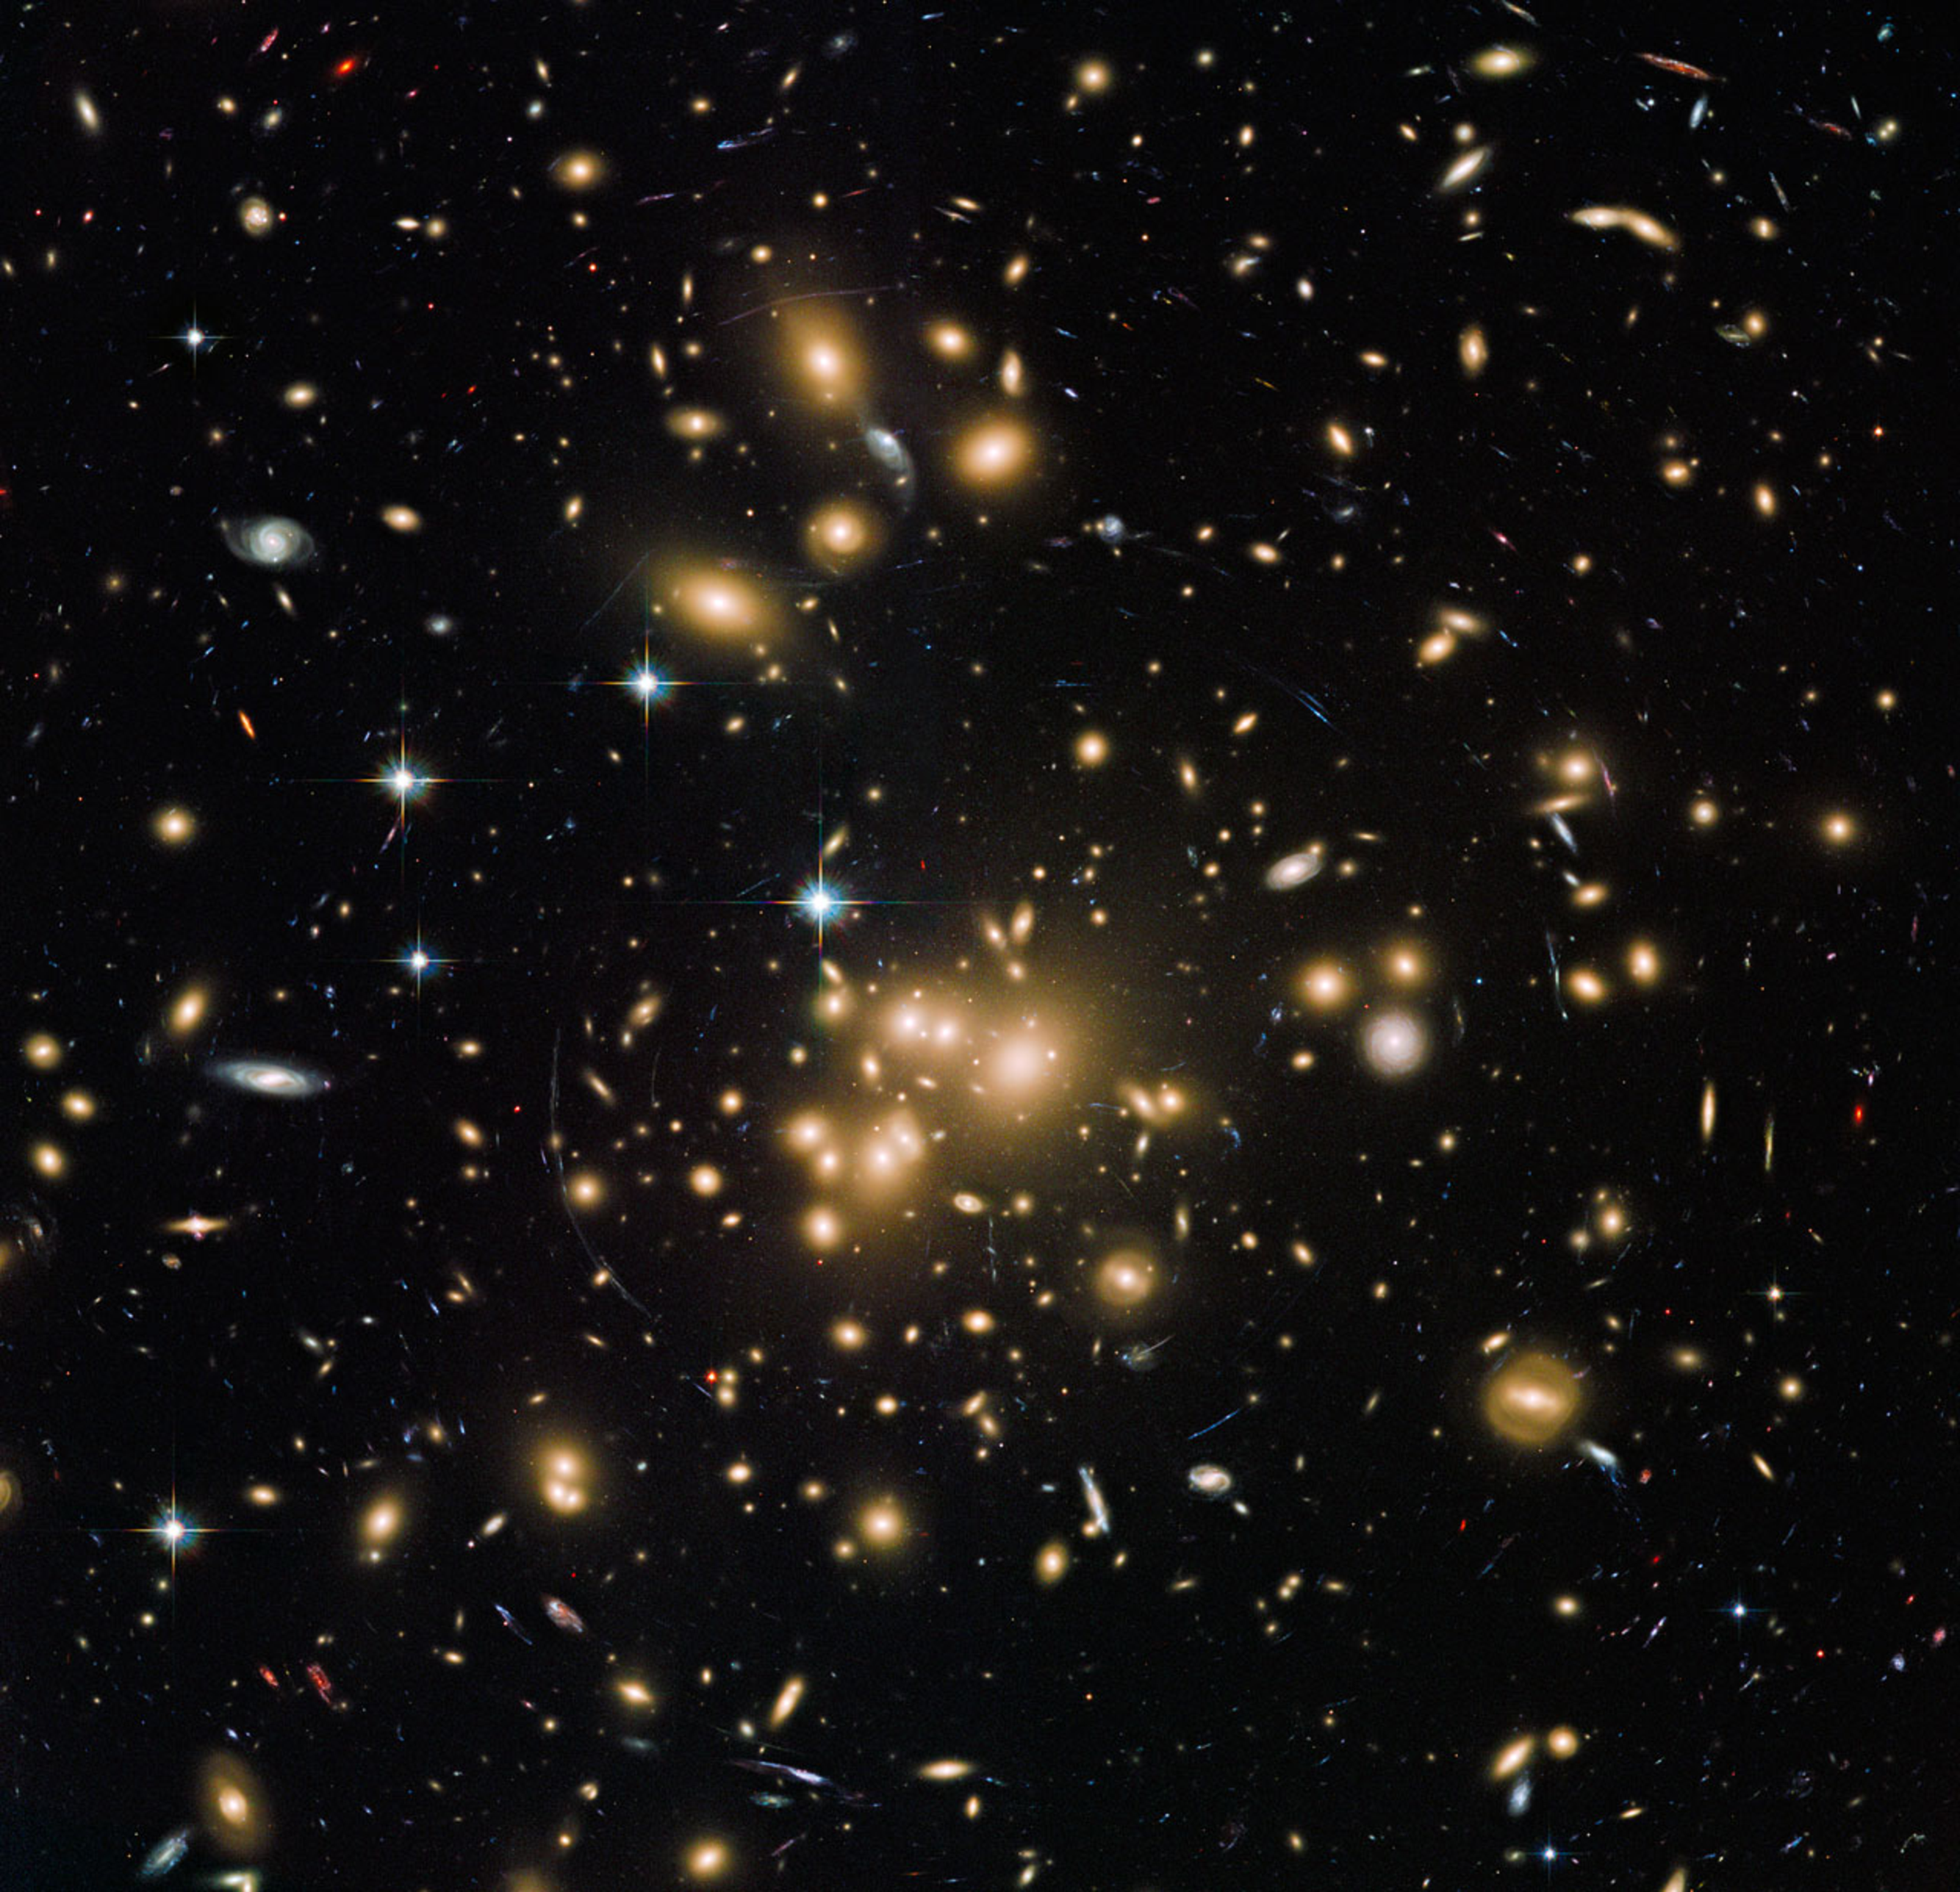
\includegraphics[width=0.6\textwidth]{figures/abell1689_hubble.pdf} 
	\end{center}
	\caption[Hubble Space Telescope image of galaxy cluster Abell 1689.]{Hubble Space Telescope image of galaxy cluster Abell 1689. Many of the galaxies visible are associated with the cluster. Not visible is the ICM or the larger DM halo which constitues the majority of the cluster mass. Credit: ESA/Hubble [CC BY 3.0 (http://creativecommons.org/licenses/by/3.0)]}
	\label{fig: abell1689_hubble} 
\end{figure}

Modern astronomy catalogues the composition of galaxy clusters in three main parts. The galaxies themselves comprise the most obvious feature, and contain a large portion (but not the entirety) of the luminous matter (stars) in the cluster. The intracluster medium (ICM) is the space between the cluster galaxies and is composed mainly of ordinary matter (baryons) which is super heated to tens of thousands of kelvin. The ICM contains the bulk of the cluster's baryonic matter, and while it is very hot, it is not very dense, having a typical value of $10^{-3}$ particles per cubic centimeter. The majority of the cluster's mass is located in the DM halo surrounding the cluster. For this reason, galaxy clusters are often referred to as halos, a term we use interchangeably throughout this work. Figure~\ref{fig: abell1689_hubble} shows a \emph{Hubble Space Telescope} Advanced Camera for Surveys image of galaxy cluster Abell 1689. Many of the cluster member galaxies have a similar yellow color. While the DM halo is not directly imaged, evidence for it can be seen by the very faint gravitational arcs of distant galaxies located behind the cluster.

Thought to form out of the primordial density fluctuations in the very early universe, galaxy cluster formation and growth investigations began in the 1960s. Soon thereafter, the hierarchical model of structure formation \citep{Press1974, Gott1975, White1978} was introduced. It suggests the first stars and stellar clumps were formed then subsequently merged together with dark matter and other gas clumps to form the first galaxies which then continued to merge and grow into the clusters and large scale structures we see today. This accretion of smaller systems is thought to be driven by the gravity of the DM associated with the cluster. Of course, many complicated astrophysical processes are at work during cluster growth and similarly complicated theoretical models seek to explain these processes. For a detailed review of cluster formation see \cite{Kravtsov2012}.

Because their initial seeds were planted in the very early universe, the number and distribution of galaxy clusters across the sky are the fingerprints of the cosmology imprinted on the universe at its birth. To uncover the underlying cosmology, a detailed understanding of the astrophysical processes that describe the motion of constituent galaxies and their impact on the ICM is required. Therefore, galaxy clusters stand at the intersection of cosmology and astrophysics. 

\section{Cosmology with Galaxy Clusters}
The current concordance cosmology is a parametrization of the Big Bang cosmological model where the universe contains a cosmological constant ($\Lambda$; often referred to as dark energy) and cold dark matter (CDM). It is often characterized by six parameters; the Hubble Constant ($H_0$), the baryonic matter density ($\Omega_b$), the DM density ($\Omega_c$), the dark energy density ($\Omega_\Lambda$); the normalization of the power spectrum ($\sigma_8$); and the spectral index of the power spectrum ($n_s$). 

Galaxy clusters are sensitive probes of $\Omega_m$, the total mass ($\Omega_b + \Omega_c$) density in the universe and $\sigma_8$. Galaxy clusters trace the peaks in the universal matter density, often referred to as the power spectrum of matter density fluctuations or the matter power spectrum, much in the same way islands (mountain peaks) trace land masses through the earth's oceans. We can constrain the values of $\Omega_m$ and $\sigma_8$ by comparing the number density of the observed galaxy clusters to that predicted by cosmological models.

The determination of cosmological parameters is done by comparing the number of galaxy clusters per unit mass per unit comoving volume ($n(M,z)$) to models. See \cite{Allen2011} for a comprehensive review or \cite{Murray2013} for a more practical approach. $n(M,z)$, referred to as the halo mass function (HMF) captures the number evolution through a function which defines the particular model used \citeeg{Tinker2008}. Early work by \cite{Press1974} and \cite{Bond1991} which assumed spherically symmetric halos, has largely been replaced by more modern fitting functions which, at the expense of an analytical solution, provide more accurate results when fit to simulation data. See \cite{Murray2013} for a review of the most common fitting functions used. Through this approach, the two parameters which clusters are most sensitive to, $\Omega_m$ and $\sigma_8$, are in reality measured as $\sigma_8\Omega_m^\alpha$, where the value of $\alpha$ depends on the masses of the halos considered. The degeneracy is broken through the evolution of the HMF as a function of redshift. 

The accuracy of the estimates of $\Omega_m$ and $\sigma_8$ depends on how well the observed HMF can be measured. The correctness of the HMF depends directly on the number of galaxy clusters observed and the accuracy to which the mass of each of the clusters can be estimated. As we discuss below, the identification of large numbers of clusters is not a considerable contributing factor to the uncertainty; the total number of clusters known is only increasing. The accurate recovery of galaxy cluster mass for both very rich clusters (those with high mass) and, importantly, the poor clusters (those with low mass) remains the dominate source of uncertainty \citeeg{Sehgal2011,Plank2014, Bocquet2015}.

\section{Observations of Galaxy Clusters}
Observations of galaxy clusters span almost the entire electromagnetic spectrum, from the X-ray to the radio. For our purposes we focus on three observations which are most useful for estimating cluster mass. We discuss them in order of increasing wavelength.

\subsection{X-ray}
As mentioned previously, the majority of a galaxy cluster's baryonic matter is located in the hot ICM. The gas which makes up the ICM is falling into the gravitational potential well of the cluster and is heated to tens of megakelvins. Such high temperatures cause the gas to emit X-rays through the bremsstrahlung process. The X-ray luminosity ($L_X$) of a galaxy cluster correlates with the depth of the gravitational potential well, which leads to an estimate of the cluster's mass \citeeg{Finoguenov2001}. 

The $L_X$ of a cluster is a relatively easy measurement, requiring only a few photons to measure. However, for a fixed cluster mass $L_X$ decreases quickly with increasing redshift, which limits X-ray selected samples of galaxy clusters to redshifts $< 1$. Up until today, X-ray identified clusters have mostly been observed purposefully through targeted \textit{Chandra} or \textit{XMM-Newton} observations. That is soon to change with the \textit{eROSITA} \citep{Pillepich2012} telescope onboard the Spektrum-Roentgen-Gamma Mission, which will perform an all-sky survey during its four year mission and detect an estimated 50,000 or more clusters.

\subsection{Optical}
To determine which galaxies do and do not belong to a given cluster, optical observations play a key role. This makes it possible to identify and study individual galaxies in a cluster environment; however, it can also provide an estimate of the cluster's total mass. Much like the X-ray observations, the motions of the individual member galaxies (referred to as velocity dispersion) provide an estimate of the depth of the cluster's gravitational potential well, which is an estimate of the total cluster mass. The constituent cluster galaxies act as tracer particles through the cluster's potential well. This can be modeled in simulations and has been the focus of many recent studies \citeeg{Evrard2008, Munari2013, Saro2013, Sifon2013, VanderBurg2014}. This type of measurement is important because it is independent of the physics of the ICM, which are always not fully understood. However, this type of measurement requires spectroscopy, which is expensive to obtain. 

\begin{figure}[t]
	\begin{center}
		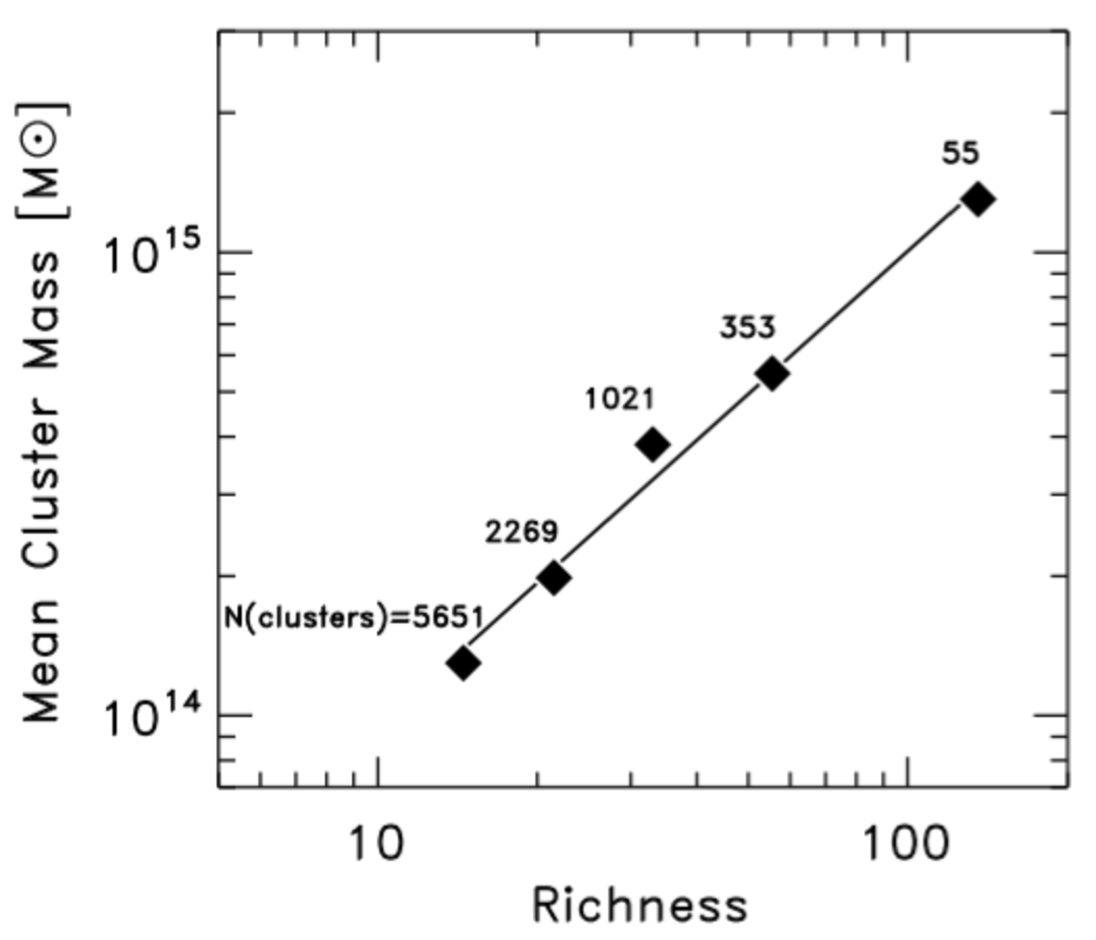
\includegraphics[width=0.6\textwidth]{figures/massrichness.pdf}
	\end{center}
	\caption{The relation between the mean Richness and the mean cluster mass.} 
	Derived from stacked weak lensing measurements and adapted from \citealt{Rozo2010}, the number of clusters in each stack are given above each data point. There is a strong correlation between richness and cluster mass, however, because the data are stacked, the absolute mass scale and scatter in mass at fixed richness are imprecisely known.
	\label{fig:massrichness}
\end{figure}

It is possible to estimate both cluster membership and mass through photometric observations alone, using modern cluster finding algorithms such as the red-sequence Matched-Filter Probabilistic Percolation (redMaPPer; \citealt{Rykoff2014}) which measures a galaxy cluster's richness. The richness measurement, in the case of redMaPPer, is a probability weighted cluster membership, where the probability is whether or not an individual galaxy belongs to the cluster in question. Figure~\ref{fig:massrichness} shows the richness correlates strongly with cluster mass on average \citeeg{Rozo2010}, but the absolute mass scale of the optical richness mass estimator and the scatter in cluster mass at fixed optical richness are imprecisely known \citep{Rykoff2012}.

Large optical surveys such as the Dark Energy Survey (DES; \citealt{DES2005}) and the Large Synoptic Survey Telescope (LSST; \citealt{LSST2012}) will survey enormous portions of the sky extremely deeply and will identify vast numbers of clusters using optical selection methods \citeeg{Rykoff2014, Rozo2014}. However, these surveys will be photometric, and any spectral information will be obtained from preexisting datasets. While it is possible to estimate cluster masses using photometric redshifts, primarily through the richness-mass relation, spectroscopic followup is required to both better calibrate the relation and to obtain the level of precision needed to compete with other mass estimators. 

\subsection{The Sunyaev-Zel'dovich Effect}
Millimeterwave observations of the Cosmic Microwave Background radiation (CMB) can show the presence of galaxy clusters. Their existence is detected through an effect called the (thermal) Sunyaev-Zel'dovich effect (SZE; \citealt{Sunyaev1972}) which is the up-scattering of CMB photons as they pass through the hot ICM. By means of inverse Compton scattering, the CMB photons receive an energy boost when they collide with the high energy electrons of the ICM. This energy boost leads to a minor blue-shift of the CMB spectrum, which is illustrated in Figure~\ref{fig:sze}. 
\begin{figure}[ht]
	\begin{center}
		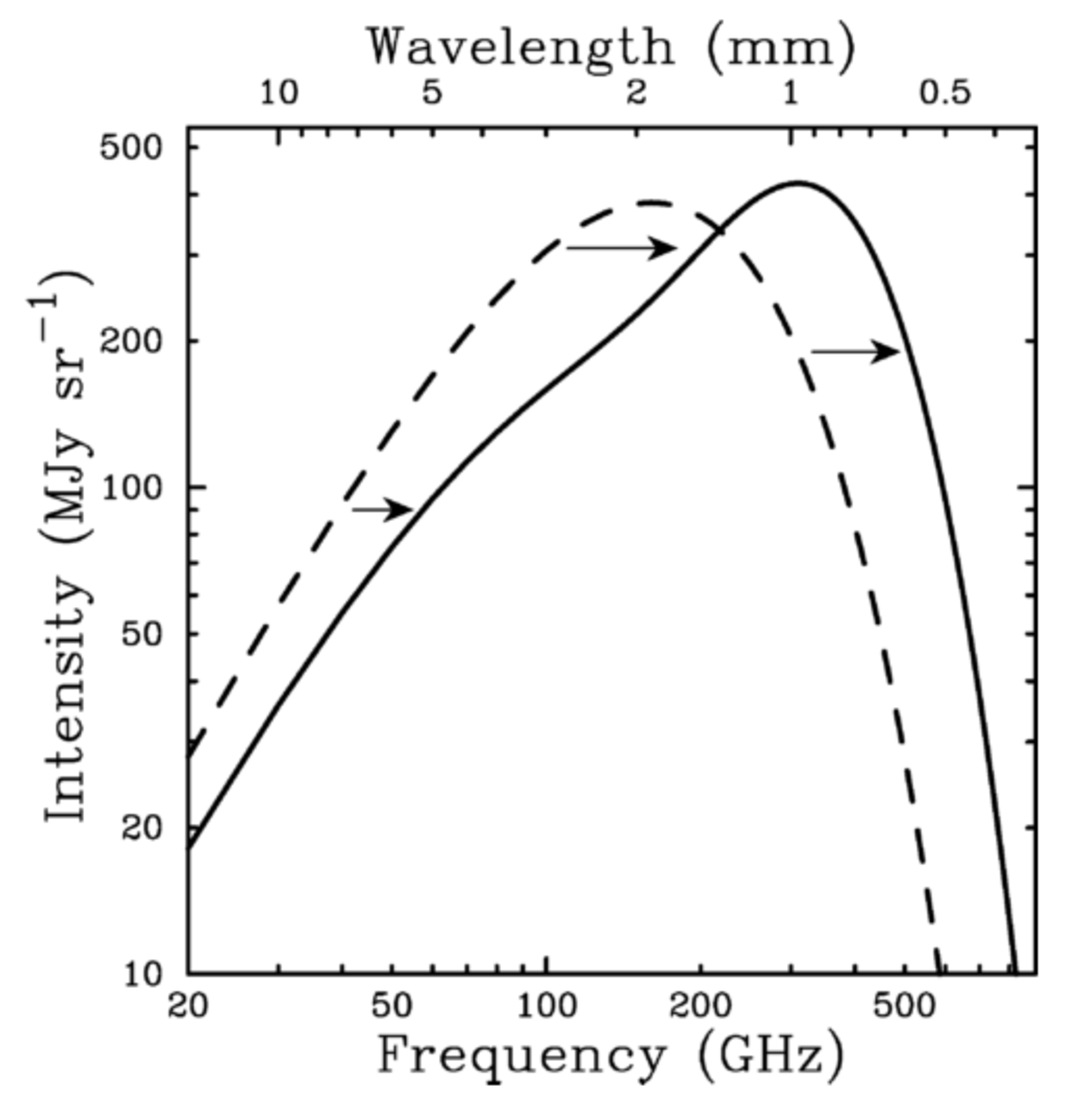
\includegraphics[width=0.6\textwidth]{figures/sze.pdf}
	\end{center}
	\caption[The Sunyaev-Zel'dovich Effect.]{Adapted from \cite{Carlstrom2002a}, the undistorted CMB spectrum (dashed line) is shifted to a higher energy (solid line) by the SZE. Note: this shift is for illustration purposes only, the SZE distortion shown is for a fictional cluster 1000 times more massive than a typical massive galaxy cluster.}
	\label{fig:sze}
\end{figure}
High resolution images of the CMB can detect a ``hole'' in the CMB at frequencies below 218 GHz, and a bright spot at higher frequencies due to the shift in the CMB black body spectrum. The temperature of the ICM effects the depth (or height) of the CMB observations, similarly to the X-ray observations, which, in turn, provides an estimate of the cluster's total mass. 

At their completion, the South Pole Telescope (SPT; \citealt{Carlstrom2011}) and the Atacama Cosmology Telescope (ACT; \citealt{Swetz2011}) are expected to find approximately one thousand clusters using observations in the millimeter combined with the SZE. Attempts are already underway to calibrate these observations using subsamples of clusters (approximately 100 cluster candidates and 60 clusters respectively) and other observables such as optically-based, virial estimates or X-ray temperature measurements \citeeg{Sifon2013, Bocquet2015}. 

\section{Galaxy Cluster Surveys as a Data Science Challenge}
Astronomy and astrophysics are undergoing a data revolution. Advances in telescope design, detectors, and computing resources have provided more astronomical data than any previous time in the history of the field. Beginning in the early 2000s, astronomical surveys have generated many hundreds of terabytes of data for many millions of sources. In the coming years, this data excess will grow beyond the terabyte regime with observations of billions of astronomical objects. 

50,000 or more X-ray identified clusters will be found by the upcoming eROSITA telescope onboard the \emph{Spektrum-Roentgen-Gamma} Mission. SPT and ACT are discovering many thousands of clusters through the SZE. DES and LSST will optically identify many tens of thousands of clusters with much lower masses than are possible with SZE measurements. Taken together, these surveys will produce data products where are both immense and heterogeneous. The multi-wavelength observations ensures there will be many observational parameters associated with each cluster. However, different observation wavelengths probe different cluster physics making them more or less sensitive probes of a specific galaxy cluster's total mass. Varying angular resolutions will also play a role as the instruments used to collect the data will observe both in a wide range of wavelength and be both ground and space based. Therefore, the combination of datasets will be a significant challenge.

The ability to associate individual or combinations of observations with the cluster property in question will be a powerful statistical tool. Combining redshift with velocity dispersion measurements could potentially produce more accurate estimates of cluster mass with smaller scatter. However, the process by which the observations are combined is not a trivial exercise. Machine learning offers a promising approach.

\subsection{Machine Learning}
Machine learning (ML) is a branch of computer science focused on the study and construction of computational tools which can learn from and make predictions based on data. In 1959, Arthur Samuel (December 5, 1901 -- July 29, 1990), an early computer gaming pioneer, described ML as a ``field of study that gives computers the ability to learn without being explicitly programmed.'' While, a great deal of programming is often required (discussed further below), such algorithms work by comparing data to a set of models allowing them to make predictions based on the data rather than preprogrammed commands.

ML can be broken into two large categories, unsupervised or supervised learning. ``Unsupervised learning'' is where the ML is tasked to make qualitative statements about the data which were not previously known. An example would be finding clusters of data inside a large dataset, where the number and location of the clusters are not known a priori (\eg, locating galaxy clusters in observations of galaxy positions; see Section~\ref{sec: future}). ``Supervised learning'' asks the computer to make predictive statements about one variable based on the observations of another or combination of variables. An example could be photometric redshift prediction; given a large number of color and magnitude measurements for a galaxy, predict the most probable redshift.  

In this work, we are concerned with supervised learning, where we know a relationship exists between two sets of data, and we use a computer algorithm to infer the relationship for us. To do this learning, we use an algorithm called decision tree learning which works by mapping a set of observations (``features'' in ML speak) of a source to a set of conclusions (``targets'') about that source. If the set of conclusions is finite, then the method becomes a classification tree; if the conclusions are infinite then it becomes a regression tree. 

\begin{figure}[ht]
	\begin{center}
		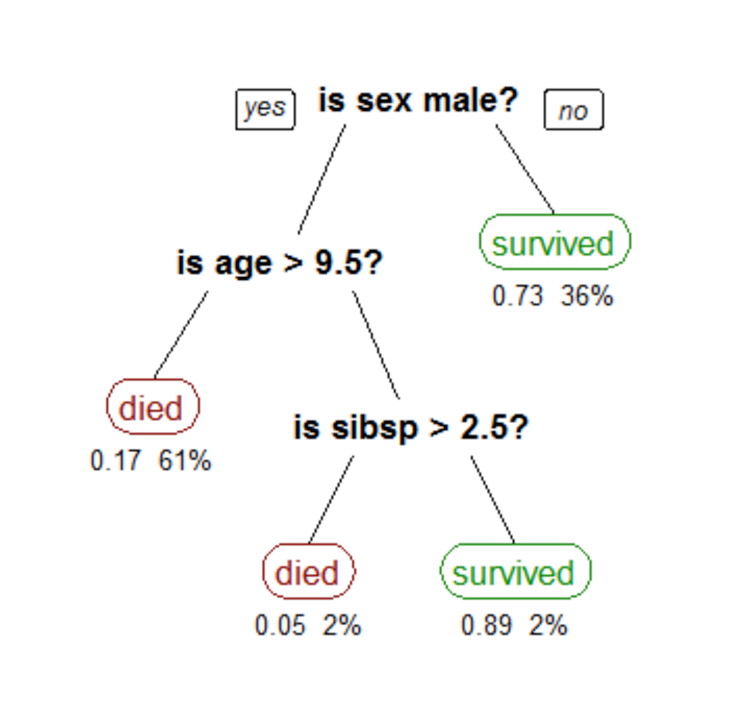
\includegraphics[width=0.6\textwidth]{figures/CART_tree_titanic_survivors.pdf} 
	\end{center}
	\caption[An example of a classification tree.]{Decision tree classifying the survival of passengers on the RMS Titanic. ``sibsp'' represents the number siblings or spouses aboard, and the numbers below each class represents the probability of survival and fraction of passengers which are classified into each leaf. Credit: Stephen Milborrow (Own work) [CC BY-SA 3.0 (http://creativecommons.org/licenses/by-sa/3.0) or GFDL (http://www.gnu.org/copyleft/fdl.html)]}
	\label{fig: cart tree} 
\end{figure}

Figure~\ref{fig: cart tree} shows a simple example of a classification tree for the survivability of passengers on the RMS Titanic. The bolded text is referred to as interior nodes which correspond to a single feature of each passenger in the example, sex, age and number of siblings or spouses. The ending points are called leaves which represent the value of the target variable given the value of the features input into the tree. For this example, there are two possible ending leaves, ``died'' or ``survived.'' Using this simple tree we are able to classify all passangers into the two possible classes. 

The ML algorithm ``learns'' this tree by choosing a feature from all available features which best splits the input data into two or more subsets. In the case of the example, this is the sex of the passenger. This becomes the root node. All subsequent nodes are created by repeating this process on each subset associated with the previous node. In such manner, it will split the male passengers by age and then by number of siblings for the males older than 9.5 years. This process is known as a top-down induction of decision trees and is the most common method for creating decision trees from data.

Once the decision tree has been learned, it can be used to classify data not seen before. For example, a 30 year-old, male passenger of the RMS Titanic has a probability of survival of 17\% and so will most likely be classified as ``died'' by the ML algorithm. However, imagine for a moment, with the benefit of hindsight that we know this male passenger survives. Only 17\% of the time will the ML method classify the passenger as ``survived'' based on this decision tree. We can boost the predictive power of the tree by generating many trees and then combining the final predictions at the end. Methods that construct more than one tree are called ensemble methods. For this work, we use an ensemble method know as a forest of randomized trees and discuss them further in Section~\ref{sec:machine learning method} and Section~\ref{2sec:ML based cluster masses}.

\section{This Work}
The goal of this work is to understand how a survey such as HETDEX can reduce the associated systematics of galaxy cluster mass scaling relations, specifically the optical richness-cluster mass scaling relation. HETDEX is a forthcoming blind spectroscopic survey that could potentially be used to accurately calibrate the richness-mass relation for a significant number of galaxy clusters at both extremes of the mass scale. The primary science mission for HETDEX is to measure the dark energy equation of state at $z\sim2$, and so the applicability to galaxy cluster science has not yet been investigated. We discuss HETDEX further in Section~\ref{sec: hetdex}.

In this thesis, we first use a set of state-of-the-art simulations where we replicate the observing strategy of HETDEX to determine the number and nature of clusters that might be observed. This is accomplished in two ways; in each part we measure the dynamical properties, such as redshift, velocity dispersion, and mass of the clusters. First we use targeted observations and perfect knowledge of the observed galaxy clusters, which includes center, membership, and number to recover the desired properties. Secondly, we assume that we know the location, but not the center, membership, or number of constituent galaxies. Then we will employ the HETDEX observing strategy, including realistic pointing pattern, observational magnitude constraints, and spectral sensitivity limits to generate a set of realistic observations.

For the two sets of observations, we use three methods to estimate each galaxy cluster's mass; a traditional power law method, a probability based method, and a ML based approach. Then, using those cluster mass estimates, we attempt to characterize the richness-mass relation (or relations) to better understand the dominate sources of uncertainty when using HETDEX like observations. This will enable us to more fully understand and constrain the HMF which, in turn, allows us to make more accurate measurements of the cosmological parameters traced by galaxy clusters.

As a practical test of the approaches we develop in the theoretical portion of this work, we use targeted spectroscopic observations of ten nearby clusters with the Mitchell Spectrograph (formerly known as VIRUS-P; \citealt{Hill2008a}), the prototype instrument for HETDEX, to estimate cluster properties. After determining cluster membership and applying many of the same cluster mass estimators as before, we again attempt to estimate the scatter and absolute scale of the optical richness-mass relationship.
 
%%%%%%%%%%%%%%%%%%%%%%%%%%%%%%%%%%%%%%%%%%%%%%%%%%%
%
%  New template code for TAMU Theses and Dissertations starting Fall 2012.  
%  For more info about this template or the 
%  TAMU LaTeX User's Group, see http://www.howdy.me/.
%
%  Author: Wendy Lynn Turner 
%	 Version 1.0 
%  Last updated 8/5/2012
%
%%%%%%%%%%%%%%%%%%%%%%%%%%%%%%%%%%%%%%%%%%%%%%%%%%%

%%%%%%%%%%%%%%%%%%%%%%%%%%%%%%%%%%%%%%%%%%%%%%%%%%%%%%%%%%%%%%%%%%%%%%%
%%%                           SECTION II
%%%%%%%%%%%%%%%%%%%%%%%%%%%%%%%%%%%%%%%%%%%%%%%%%%%%%%%%%%%%%%%%%%%%%%

\renewcommand*{\thefootnote}{\fnsymbol{footnote}}
\chapter[Chapter1]{\uppercase {Chapter1}\symbolfootnote[1]{Reprinted with permission from ``Introduction: The Importance of Research'' by AUTHOR et al., 2015. The Astrophysical Journal, Volume XYZ, Issue X, article id. XY, XY pp., Copyright 20XX by the American Astronomical Society.} }
\renewcommand*{\thefootnote}{\arabic{footnote}}
\setcounter{footnote}{0}

\section{Introduction}\label{sec: Introduction}
Our ability to perform precision cosmology with clusters of galaxies has reached a critical point. The widely accepted $\Lambda$CDM model of cosmology makes explicit predictions about the mass function of galaxy clusters in the universe. Measuring this mass function across many redshifts, in turn, provides constraints on the cosmology. Today, large-area sky surveys are providing observations of large numbers of clusters, but systematics in deriving cluster masses dominate the error budget \citeeg{Sehgal2011,Plank2014, Bocquet2015}. To place further constraints on the $\Lambda$CDM model of cosmology, we must decrease these systematics. 

As mass is not a direct observable, a lot of work is underway to characterize galaxy cluster masses with an observable feature of galaxy clusters. The goal is to constrain $P(M|z, \vec{x})$ the probability density ($P$) that a galaxy cluster of given mass ($M$), located at redshift ($z$) determined using an observable parameter or parameters ($\vec{x}$). Generally, cluster mass calibrations are done in one of two ways, through simulations or direct or statistical calibration.

One could use various simulations to attempt to calibrate this observable-mass relation \citeeg{Vanderlinde2010, Sehgal2011}. However, the primary challenge to this method is the incomplete understanding of the baryonic physics which take place in galaxy cluster environments. While there have been (and continue to be) many improvements in the accuracy and power of simulations it is doubtful that in the coming years they will reach the accuracy level required where the observable--mass relation is dominated only by statistics \citep{Weinberg2013}. 
 
The second broad method is the direct calibration of cluster masses. This recipe has two distinct but not always independent tracks. The ``direct'' method uses observations of a relatively small set of clusters and then uses known mass estimators, including X-ray temperatures and luminosities \citeeg{Mantz2010, Rykoff2014}, microwave observations \citeeg{Vanderlinde2010, Sehgal2011}, optical richness \citeeg{Abell1958, Rykoff2012} or weak lensing (WL; \eg\ \citealt{Rozo2010}) as examples, which provide a ``true'' mass. This directly calibrates the observable-mass relation which is then applied to a much larger sample. The complications lie in that the ``true'' masses are, in fact, estimations, and the methods used to recover these cluster masses are subject to their own limitations. X-ray based cluster masses assume hydrostatic equilibrium \citeeg{Mantz2015} which may only be valid for a very small number and range of cluster masses. The Sunyaev-Zel'dovich Effect (SZE; \citealt{Sunyaev1972}), which uses the up-scattering of cosmic microwave background (CMB) photons to estimate cluster masses, provides accurate estimations of mass, but the ability to detect low mass galaxy clusters is currently limited by technology \citeeg{Carlstrom2002a} and can also be effected by the properties of the intracluster medium \citeeg{Pipino2010}. WL estimates are, in principle, correct in the mean, but they suffer from signal-to-noise requirements, limiting their usefulness in low mass clusters (where the lensing signal is particularly weak), and potentially suffer from line-of-sight effects as WL is sensitive to all mass along the line-of-sight. Virial mass estimators which determine the cluster mass based on the motions of the member galaxies \citeeg{Ruel2014, Sifon2015} are promising in that it is a direct measurement of the depth of clusters potential well, but suffer from systematics due to cluster formation physics which disrupts the velocity field.
 
The statistical method of determining galaxy cluster mass relies not on direct measurements of individual clusters but the calibration of observables for the entire sample which correlate with cluster mass. One example is the spatial clustering of the galaxy clusters themselves \citeeg{Baxter2016}. See \cite{Weinberg2013} for a comprehensive review. In practice, it will be a combination of the three methods touched on that will provide the most reliable determination of cluster masses.

Large-area sky surveys, both on going and planned, are revolutionizing cluster cosmology using a large range of wavelengths. The South Pole Telescope (SPT; \citealt{Carlstrom2011}) and the Atacama Cosmology Telescope (ACT; \citealt{Swetz2011}) are discovering many clusters through the SZE. Optically, the on going Dark Energy Survey (DES; \citealt{DES2005}) and planned Large Synoptic Survey Telescope (LSST; \citealt{LSST2012}) will identify many thousands of clusters to much lower masses than is possible with SZE measurements. However, regardless of the discovery method used, spectroscopic follow-up is needed to further constrain $P(M|z,X)$. This follow-up becomes increasing important to help constrain the scatter in the mass estimates of other methods, and provides an additional, independent check of the observable-mass relationship used. But as the cluster dataset grows to many tens of thousands of clusters individual follow-up becomes increasingly impractical. Therefore, large spectroscopic surveys are needed to more fully understand the observable-mass relation of clusters.

The Hobby Eberly Telescope Dark Energy eXperiment (HETDEX; \citealt{Hill2008}) is a trailblazing effort to observe high-redshift large scale structures using cutting edge wide-field integral field unit (IFU) spectrographs. Designed to probe the evolution of the dark energy equation of state etched onto high redshift ($z>2$) galaxies by the Baryon Acoustic Oscillations (BAO) \citep{Eisenstein2005} in the first moments of the universe, the survey will observe two fields for a total of 420 \degsq\ (300 \degsq, Spring field and 120 \degsq, Fall field). Tuned to find \lya\ emitting (LAE) galaxies at $1.9<z<3.5$, HETDEX expects to find 800,000 LAEs, and more than one million \hbox{[\ion{O}{ii}]} emitting galaxies at $z<0.5$ masquerading as high-redshift galaxies \citep{Acquaviva2014}. 

While a large portion of the $\sim10^6$ interloping lower redshift galaxies will be field (not associated with a bound structure) galaxies, the large area covered by HETDEX is expected to contain as many as 50 Virgo-sized (halo mass $>10^{15}$ \msol) clusters at $z<0.5$. The near-complete spectroscopic coverage allows an unprecedentedly detailed look at a very large number of clusters ranging from group scales to the very massive. In addition to the recovery of accurate dynamical masses, detailed investigations of the of dynamical state of the clusters is possible. 

It is unclear how a blind spectroscopic survey with an IFU will effect the recovery of galaxy cluster dynamical properties. Unlike many previous large cluster surveys \citeeg{Milvang-Jensen2008, Robotham2011, Sifon2015} which use multi-object spectrographs, the Visible Integral-Field Replicable Unit Spectrograph (VIRUS; \citealt{Hill2012}) used by HETDEX samples the sky in a uniform but sparse way which could excluded member galaxies which would otherwise be included. Secondly, it is not straightforward to use spectroscopic redshifts predominately from emission-line galaxies to interpret the kinematic and dynamical states of the clusters.

\begin{figure*} 
	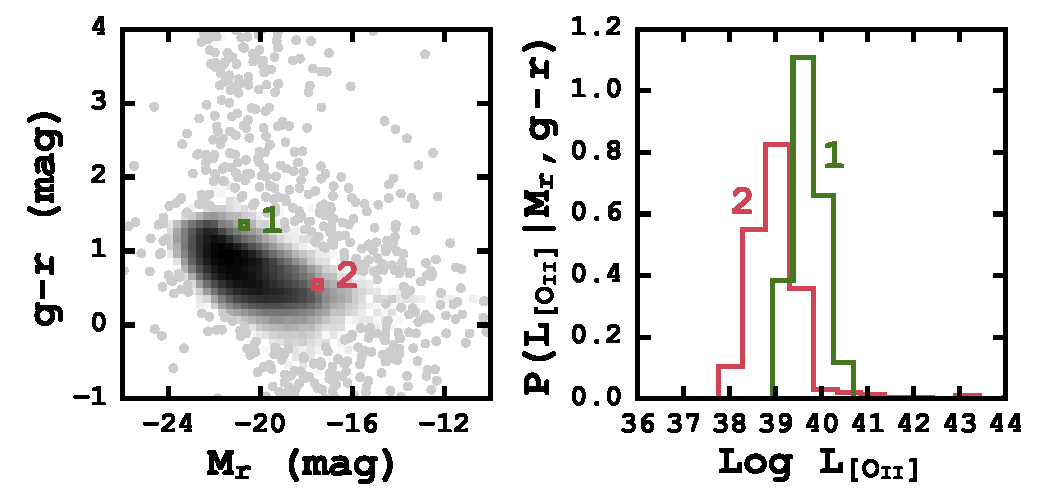
\includegraphics[width=0.9\textwidth]{figures1/oii_sdss.pdf} 
	\caption{\textit{Left}: CMD of 503,113 $z<0.2$ galaxies take from the SDSS DR12 where the shading scales with the density of points. The two colored boxes show regions containing potential catalog galaxies. \textit{Right}: Probability histograms of the Log \hbox{[\ion{O}{ii}]} luminosity for the SDSS galaxies located in the two highlighted regions on the right. The \hbox{[\ion{O}{ii}]} luminosities are assigned to catalog galaxies from slice sampling the probability histogram and converted to fluxes using the redshift of each galaxy.} \label{fig: oii sdss} 
\end{figure*}

This work plans to address these concerns in the following ways. We create and evaluate a HETDEX like selection ``function'' of galaxies over a similarly large portion of the sky and use well adopted techniques to recover the dynamical properties, such as velocity dispersion and cluster mass. In addition to standard techniques of cluster mass estimation, we investigate probability based and machine learning based approaches of cluster mass prediction. We compare these results to a series of targeted galaxy cluster observations, where each member galaxy is assumed to be observed. Each of these observations use realistic uncertainties from galaxy magnitude and line-flux limits. These strategies will better allow future work to predict the number and types of galaxy clusters which should be observed with VIRUS during both the HETDEX survey portion and through targeted follow up observations.

We begin in Section \ref{sec:Data} by giving an overview of what data is used, how it is created, and how we make our ``observations.'' Details about the determination of cluster parameters, velocity dispersion, total mass, etc., are discussed in Section \ref{sec:recovery}. Next, we present the results of our study in Section \ref{sec:results} and discuss their implications in Section \ref{sec:discussion}. Finally we summarize our findings in Section \ref{sec:summary}. A follow-up to this work \citep{Boada2016a} will investigate how the techniques developed here will work in practice. 

Throughout this paper, we adopt the following cosmological model: $\Omega_\Lambda = 0.714$, $\Omega_M = 0.286$, $\sigma_8 = 0.82$ and $H_0= 70$ \kms \mpc (taken from the Buzzard catalogs; see below), assume a Chabrier initial mass function (IMF; \citealt{Chabrier2003}), and use AB magnitudes \citep{Oke1974}.

\section{Data and Mock Observations}\label{sec:Data}
In this section, we describe the data products and the techniques used to replicate the HETDEX survey. We use the information from a large mock galaxy catalog enhanced by the emission line properties of galaxies in the SDSS to create a realistic ``sky'' and ``observe'' it with a HETDEX-like observing strategy.

\subsection{The Buzzard Mock Catalogs}
The Buzzard mock galaxy catalogs cover 398.49 \degsq\ between $4^h< RA < 6^h$ and $-61\degree < DEC < -41\degree$ and are derived from a combination of Sub-halo Abundance Matching (ShAM) and ADDSEDs (Adding Density Dependent Spectral Energy Distributions) tied to an in house n-body cosmological simulation. A brief description of the catalog creation is described as follows. The initial conditions are generated with a second-order Lagrangian perturbation theory using {\sc 2LPTic} \citep{Crocce2006}. Dark matter (DM) n-body simulations are run using {\sc LGadget-2} (a version of {\sc Gadget-2}; \citealt{Springel2005}). The Buzzard catalogs adopt the following cosmological parameters: $\Omega_m = 0.286$, $\Omega_\Lambda = 0.714$, $H_0 = 70$ \kms \mpc, $\sigma_8 = 0.82$, and $n_s = 0.96$. The DM halos are identified using the {\sc ROCKSTAR} halo finder \citep{Behroozi2013} which also calculates halo masses. 

Galaxy $M_r$ luminosities are added to the velocity peaks using ShAM \citep{Reddick2013}, and ADDSEDs assign luminosities in the other bands. A $M_r$-density-SED relation is created using a SDSS training set, and for each mock galaxy the SED of a randomly selected training set galaxy which has a similar $M_r$ and density is assigned. The result is a mock catalog containing 238 million galaxies with $\sdssr < 29$ mag and $z \leq 8.7$.

The catalog information, used in this study, is broken into two large portions. The ``truth'' files contain the characteristics of each individual galaxy, such as right ascension (RA), declination (DEC), redshift ($z$), observed and rest-frame magnitudes, and many others. The ``halo'' files contain information for individual halos, to which many individual galaxies may belong. This includes five estimations of dynamical mass, RA, DEC, z, three dimensional velocity dispersion, and many others. However, the catalogs do not include information for emission lines. We supplement the catalogs by generating this information; the process is described in Section~\ref{sec: oii luminosity}.

% \begin{figure}
% 	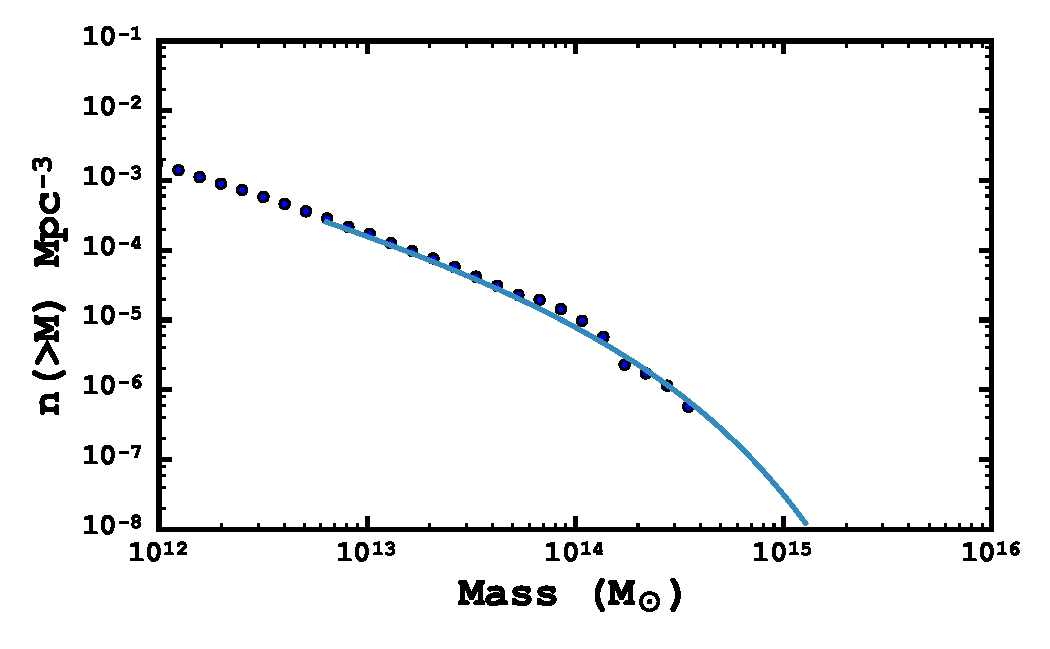
\includegraphics[width=\textwidth]{figures1/hmf.pdf}
% 	\caption{The cumulative MF (from \citealt{Tinker2008}) of halos above $M_{200c}$ at $z=0.1$}
% 	\label{fig: hmf}
% \end{figure}

We investigate the accuracy of the halo mass distribution by comparing the cumulative number density of halos above a mass ($M_{200c}$) threshold to the halo mass function (HMF) of \cite{Tinker2008}. We calculate the HMF at central redshifts of 0.1, 0.2, and 0.4 using {\sc HMFcalc} \citep{Murray2013} and compare it galaxies in a redshift window of $\Delta z\pm0.01$. We find a very good agreement between the predicted HMF and the observed distribution of clusters.

\subsection{Conditional \hbox{[\ion{O}{ii}]} Flux Probability Distribution Functions}\label{sec: oii luminosity}
We use the SDSS DR12 \citep{Alam2015} catalogs to assign \hbox{[\ion{O}{ii}]} emission line strengths to the galaxies in the Buzzard catalog. We use 503,113 objects classified as galaxies selected over $z = 0.02 - 0.2$ with {\sc zwarning $=0$} and a measured \hbox{[\ion{O}{ii}]} line flux signal-to-noise of five. Figure~\ref{fig: oii sdss} shows the color-magnitude diagram (CMD) of $M_r$ and $g-r$ for these galaxies.

To assign an \hbox{[\ion{O}{ii}]} luminosity to each galaxy in our catalog, we place the catalog galaxies on the same CMD and select all SDSS galaxies in a small 2D ($M_r$, $g-r$) bin around the galaxy. We extract all of the SDSS galaxies inside that bin and create a histogram of their \hbox{[\ion{O}{ii}]} luminosities, the right panel of Figure \ref{fig: oii sdss}. Using a slice sampling technique \citep{Neal1997} we assign the catalog galaxy an \hbox{[\ion{O}{ii}]} luminosity based on the distribution of SDSS galaxies in that bin. In very few cases (1.3\% of galaxies) do the $g-r$ and $M_r$ magnitudes of the galaxies in the Buzzard catalog not overlap with the distributions in SDSS. For these objects, we assign them zero \hbox{[\ion{O}{ii}]} flux, but this has no impact on our analysis. For catalog galaxies with have very few ($1\leq N<10$) SDSS galaxies in their respective bin, we assign it the mean \hbox{[\ion{O}{ii}]} flux. 

Figure~\ref{fig: oii sdss} illustrates this process. The numbered boxes in the left panel show the bins corresponding to two example Buzzard galaxies ($M_r, g-r = -17.7,~0.49$ and $M_r, g-r = -21.4,~1.24$). The right panel shows the Log \hbox{[\ion{O}{ii}]} luminosity distribution functions, $P($\hbox{[\ion{O}{ii}]}$| M_r, g-r)$, which we use to assign \hbox{[\ion{O}{ii}]} luminosity to each object. The luminosity is then converted into an \hbox{[\ion{O}{ii}]} flux through 
\begin{equation}
	F = \frac{L}{4\pi D_L}
\end{equation}
where $D_L$ is the luminosity distance \citeeg{Hogg1999}.

\subsection{HETDEX}\label{sec: hetdex}
\begin{figure} 
	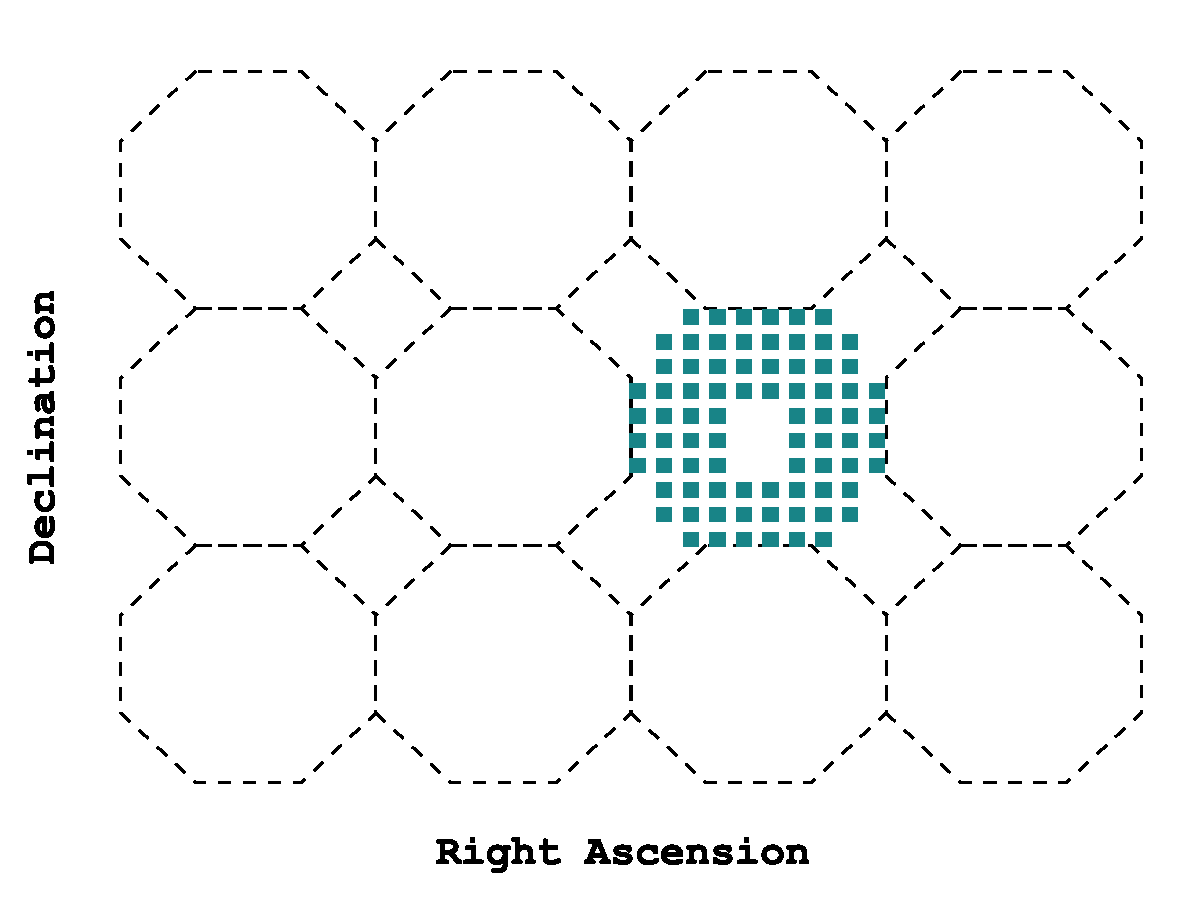
\includegraphics[width=\textwidth]{figures1/pointings.pdf} 
	\caption{Representative observation tiling scheme for the HETDEX $16' \times 16'$ pointings. Each turquoise square represents the position of a single VIRUS IFU, and the dashed octagons approximate the size of a single observation. Inside each IFU HETDEX will achieve near complete coverage through three dithers. See the text for more details.} \label{fig: ifu layout} 
\end{figure}

We designed the results of this study to be used in conjunction with HETDEX, a large, blind, spectroscopic survey. HETDEX will measure the redshifts of $8 \times 10^5$ LAE galaxies between $1.9 < z < 3.5$ using a collection of 78 wide-field IFU spectrographs covering the wavelength region $3500 - 5500$~\AAA\ at R $\sim$ 750 \citep{Hill2008}. The primary science goal of these observations is to provide $<1\%$ accuracy measurements of the Hubble expansion parameter and the angular diameter distance at $z\sim2$. This result will provide significant constraints on the evolution of the dark energy equation of state which is both competitive with, and independent of, constraints derived from observations of the \lya forest.

The entire HETDEX survey will cover 420 \degsq\ with a 1/4.5 filling factor over two fields: a $\sim 300$ \degsq\ northern field, and a $\sim 140$ \degsq\ equatorial region. The spectral coverage allows for the detection of \hbox{[\ion{O}{ii}]} ($\lambda\lambda 3727,3729$) emitters to $z\sim 0.5$ and Ca H ($\lambda 3968.5$) and K ($\lambda 3933.7$) absorption features to $z\sim 0.4$. The $10 \sigma$ detection threshold for spectral features will be $3.5\times10^{-17}$ \ergscm\ at 5000 \AAA, or equivalently, $g = 21.9$ mag for continuum objects. 

The HETDEX IFU pattern is illustrated in Figure~\ref{fig: ifu layout} by the turquoise squares. Each of the 78 IFUs, are comprised of 448 optical fibers subtending a $50'' \times 50''$ region on the sky \citep{Kelz2014}. The inter-IFU spacing is also $50''$, spanning a total area of $16'\times 16'$ on the sky. The individual IFUs have a fill-factor of 1/3, which will be completely filled with three dithers of the telescope at each pointing.

\subsection{Mock Observations}\label{sec: observations}
When selecting galaxies from the Buzzard catalog we assume an observation for all galaxies laying within a turquoise, IFU square in Figure~\ref{fig: ifu layout}. In practice, this is achieved by three dither positions at each pointing. Galaxies which lie between the IFUs are missed, as well as the galaxies which lie between the pointings, as there is no overlap between one pointing and the next. To cover the 398.49 \degsq\ field of the Buzzard catalog we require 5370 pointings where 0.015 \degsq\ of each pointing is covered by an IFU. The total area of the sky covered by an IFU is 80.80 \degsq\ which gives a filling factor of 1/4.65, slightly decreased from the expected filling factor of 1/4.5.

In this work we consider two separate observing strategies, Targeted and Survey. The Targeted observations use ``direct'' observations where each cluster is targeted individually, and every cluster member galaxy is assumed to be observed. The Survey observations mimic the HETDEX observation pattern across the sky, where no cluster is directly targeted and not all cluster member galaxies are observed. Both of these observations have HETDEX-like galaxy detection thresholds (described in the previous subsection), so while a galaxy may be observed, a redshift will only be measured if the galaxy satisfies the continuum brightness or emission line flux limits for the HETDEX survey. For comparison we also include a set of Targeted observations with ``perfect'' knowledge which assume no detection threshold, if a cluster member galaxy is observed, it is also detected. This provides an important best-case scenario, and differs from the true cluster properties between we are still calculating the cluster mass from the observed member galaxy velocity dispersions, and represent the best possible mass estimates using velocity dispersion as the observable. These observations provide three levels of quality with ``Perfect knowledge'' being the highest and Survey being the lowest.

\section{Recovery of Parameters}\label{sec:recovery}
In the following subsections, we outline the methods we use to derive the dynamical properties of the galaxy clusters in our sample. The following is, in many cases, a subset of the available methods to derive any single parameter. The specific choice of method may improve or diminish the accuracy of the recovered parameter, but the methods chosen were to facilitate comparison with other observational studies \citeeg{Kirk2015, Boada2016a}. 

\subsection{Cluster Redshift}
The accurate determination of the cluster redshift ($z_c$) is crucial to the reliability of all following measurements. An incorrect cluster redshift introduces error into the measured line-of-sight velocity (LOSV) and corresponding dispersion, which, in turn, contributes to errors associated with dynamical mass and radius. 

In simple terms, the cluster redshift is the mean of the redshifts of all galaxies associated with the cluster, where the mean is the first moment of the velocity (redshift) distribution function $P(z)$. In practice, the first moment is strongly subject to outliers, so we rely instead on the biweight location estimator \citep{Beers1990} through\footnote{Implemented as part of the {\sc astLib} Python library. See \hbox{http://astlib.sourceforge.net}}:
\begin{equation}
C_{BI} = M + \frac{\sum_{|u_i| < 1} (z_i - M)(1-u_i^2)^2}{\sum_{|u_i| < 1}(1-u_i^2)^2}
\end{equation}
where $z_i$ are the individual redshifts, $M$ is the median redshift and $u_i$ is given by:
\begin{equation}
	u_i = \frac{(z_i - M)}{C\,\mathrm{MAD}}.
\end{equation}
MAD is the median absolute deviation, also defined in \cite{Beers1990}, and $C$ is the a tuning constant. We choose $C=6$ (the suggested value) which balances computational speed and location accuracy. 

Although this work assumes that we know each galaxy's redshift to infinite precision, in practice, we find a simple weighted mean provides a reliable estimate of $z_c$ when there are uncertainties on the individual galaxy redshifts. 

\subsection{Line-of-Sight Velocity Dispersion}\label{sec: LOSVD}
We calculate the LOSV to each galaxy, where
\begin{equation}
	\mathrm{LOSV} = c\frac{z - z_c}{1+z_c}
\end{equation}
and $c$ is the speed of light, $z$ is the redshift of the individual galaxy, and $z_c$ is the overall cluster redshift described in the previous subsection.

We follow the maximum likelihood method of \cite{Walker2006} to estimate the line-of-sight velocity dispersion (LOSVD). We maximize the probability function 
\begin{equation}\label{eq: jointGaussian}
P(\{v_1, ..., v_N\})=\displaystyle\prod_{i=1}^{N}\frac{1}{\sqrt{2\pi(\sigma_i^2+\sigma_{1D}^2)}}\exp\biggl[-\frac{1}{2}\frac{(v_i-\langle u \rangle)^2}{(\sigma_i^2+\sigma_{1D}^2)}\biggr]
\end{equation}
where $\sigma_{1D}$, $\langle\mu\rangle$, and $\sigma_i$ is the LOSVD, the average radial velocity and the error on the individual LOSVs (which we have assumed to be normally distributed) respectively, using a Monte Carlo Markov Chain (MCMC) sampler ({\sc emcee}\footnote{http://dan.iel.fm/emcee/current/}; \citealt{Foreman-Mackey2013}) which is based on affine-invariant ensemble sampler (see \citealt{Goodman2010} for details on affine-invariant samplers). We draw twenty thousand samples from the posterior probability distribution using simple priors, $\langle\mu\rangle$ lies between the maximum and minimum LOSV and $0< \sigma_{1D} < 1400$ \kms. We set the upper limit on the LOSVD as the LOSVD corresponding to a $10^{16}$ \Msol\ cluster at $z\sim0.0$, higher mass than any expected cluster in Buzzard. When the full distribution of LOSVDs is not used, the final LOSVD is quoted as the median value of the posterior probability distribution with 68\% error bars defined as the square root of second moment of the same distribution, the standard deviation.

In principle, a single statistic such as the biweight scale estimator or the gapper estimator (both from \citealt{Beers1990}) with many bootstrap resamplings could be used to construct a distribution of $\sigma_{1D}$. In simple tests where the values of both $\sigma_{1D}$ and $\langle\mu\rangle$ are known, the 68\% error bars derived from the MCMC method give slightly better results with the true LOSVD value bracketed by the error bars in $\sim68\%$ of the cases versus $\sim57\%$ with bootstrapping and a single statistic. In addition, we prefer the maximum likelihood method for its straight forward treatment of the errors in the LOSV measurements, which will become important in the practical application to real data \citeeg{Boada2016a}.

\subsection{Estimates of Cluster Mass}\label{sec: mass}
\subsubsection{Power Law Based Method}
The relationship between the LOSVD and cluster dynamical mass has been the focus of several many \citeeg{Evrard2008, Saro2013, Sifon2013, VanderBurg2014}, where the relationship for the mass enclosed by $r_{200c}$ takes the form
\begin{equation}\label{eq:power law}
	M_{200c} = \frac{10^{15}}{h(z)} \bigg{(}\frac{\sigma_{1D}}{A_{1D}} \bigg{)}^{1/\alpha} \Msol
\end{equation}
with $A_{1D} = 1177 \pm 4.2$ \kms\ (\citealt{Munari2013}; referred to as $\sigma_{15}$ in \citealt{Evrard2008} and other works), $\alpha = 1/3$, $h(z) = H(z)/100$, and $\sigma_{1D}$ is the LOSVD of the velocity tracers (dark matter particles, subhalos or galaxies). $H(z) = H_0 E(z)$ and $E(z) = \sqrt{\Omega_m(1+z^3)+\Omega_{\Lambda}}$.

A growing body of work suggests that there is a significant difference in the observed LOSVD depending on the velocity tracers used. Specifically, while there is little difference between using galaxies and their host DM subhalos, there is a significant over estimation of the LOSVD when using galaxies/subhalos compared to DM particles \citep{Munari2013}. We follow other works \citeeg{Kirk2015, Sifon2015a} using the scaling relation, given in Equation~\ref{eq:power law} to facilitate comparisons with other observational studies, which rely on galaxies as tracers. 

\subsubsection{Other Estimates of Dynamical Mass -- Introduction}
In the following subsections we use two methods to predict the mass of a cluster based on other observables. Often the cluster mass is estimated based on a single observable, X-ray temperature, LOSVD, richness and others (see Section~\ref{sec: Introduction} for referenced examples). Here we combine many observables to attempt to correct the mass inferred solely from the velocity dispersion. The first method is traditional ``probability based'' where we marginalize over a series of observables to find the most probable cluster mass. The second is based on a machine learning (ML) algorithm which attempts to infer the relationship between the observables and the desired output, the cluster mass. Both of these methods are examples of supervised learning algorithms where the relationship between the observable parameters and the target parameter (the cluster mass) are both known.

As with any predictive analysis it is important to test the model on data that the model has not seen before. This prevents over-fitting. In the following subsections we take all of the observed clusters, our full sample, split them, and generate a \emph{training} and \emph{testing} set \citeeg{Ripley2007, Xu2013, Ntampaka2015, Ntampaka2015a, Acquaviva2016}. Traditionally, the training set is a set of data used to infer possibly predictive relationships. The test set of data is then used to assess the correctness of the predictive relationship. Our data is randomly split into 70\% training and 30\% testing. We follow the ML convention and refer to the individual clusters in each set as a ``sample'', and the parameters associated with the cluster ($z$, LOSVD, mass, etc.) as ``features''.

\subsubsection{Probability Based}\label{sec:probability method}
For internal consistency between this and the ML based method we use 70\% of the clusters to establish a conditional probability density of $P(M_{200c} | \vec{x})$ which we then use as the cluster mass probability density for the remaining clusters with similar features. In this way we, ``train'' the probability density using the existing simulated data, and apply it to the ``test'' sample (the remaining 30\% of the data not used as the training set).

\begin{figure*} 
	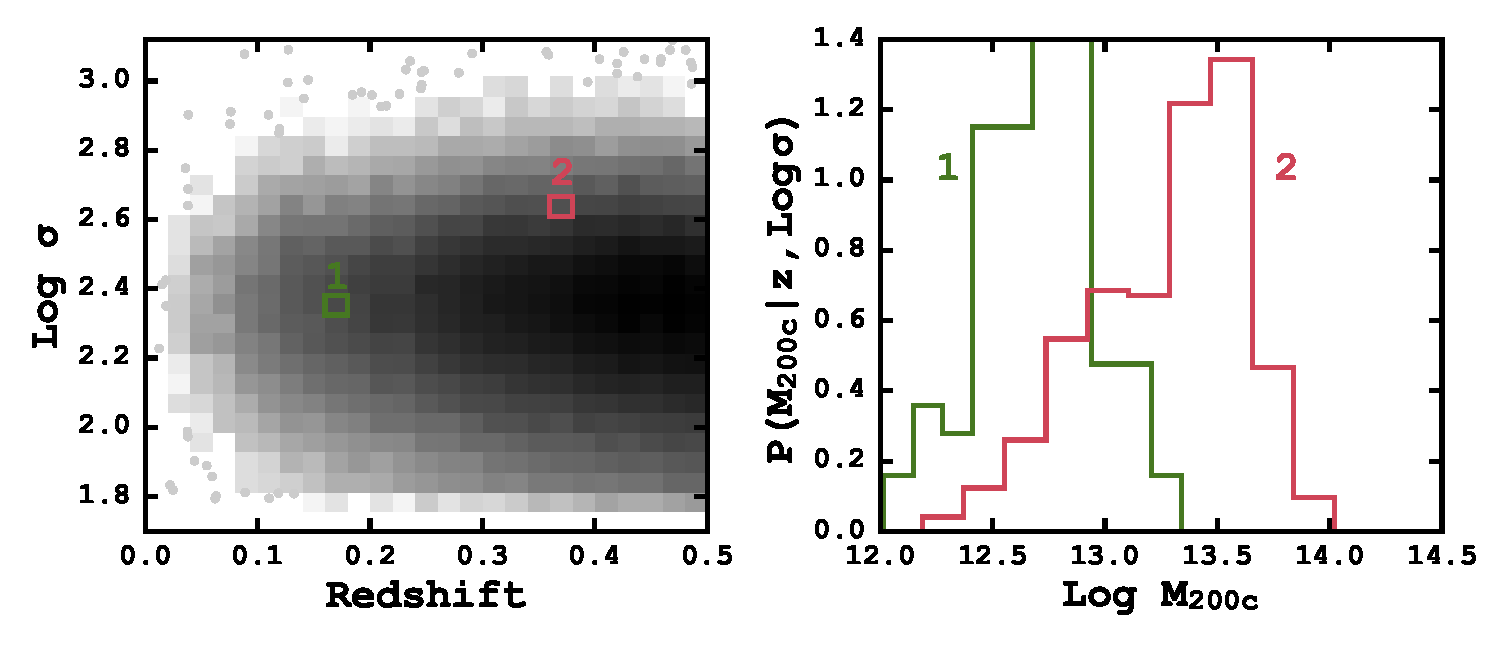
\includegraphics[width=\textwidth]{figures1/prob_example.pdf} 
	\caption{Illustration of the probability based cluster mass prediction method. \emph{Left}: The two dimensional posterior probability distribution of LOSVD and redshift used to determine the correct cluster mass. The pink and green rectangles show the locations of two example galaxies used to create the conditional probability distribution of the mass, $P(M_{200c}|\vec{x})$. \emph{Right}: The conditional probability distribution of the cluster mass for the two example galaxies. See text for a complete description.} \label{fig: probability corner} 
\end{figure*}

In this method, the cluster masses are predicted using the method illustrated in Figure~\ref{fig: probability corner}. The left panel shows the two dimensional (joint probability) projections of the posterior probability distributions of the feature training data. The conditional probability of the cluster mass $P(M_{200c}|\vec{x}= \{ x_1,x_2,...\})$ (shown in the right panel) is determined by selecting a region in the joint probability distribution. For example, using the LOSVD and redshift features we create $P(M_{200c}|\vec{x})$ for two test galaxies, shown by the green and pink boxes in the left panel of Figure~\ref{fig: probability corner}. These example galaxies have features $\vec{x} = \{\sigma=200\, \kms,z=0.16\}$ and $\vec{x} = \{\sigma=400\, \kms,z=0.36\}$. We select all galaxies in our training sample with similar features and create the conditional probability distributions shown in the right panel.

For the clusters making up the \emph{test} sample the mass is unknown (it is what we are trying to predict) but the other features are known. To determine the mass probability distribution of a test cluster, $P(M_{200c})$, we combine the conditional probability distribution, $P(M_{200c}|\vec{x})$, created previously with the probability distribution of $\sigma$, the LOSVD, through Equation~\ref{eq: Pm}.
\begin{equation}\label{eq: Pm}
	P(M_{200c}) = \int P(M_{200c}|\vec{x})\ P(\sigma)\ d\sigma\ P(z)\ dz
\end{equation}
The expected mass is determined by calculating the first moment of the probability density. This becomes our ``predicted'' cluster mass, $M_{pred}$.
\begin{equation}\label{eq: expected mass}
	M_{pred}= \int M_{200c}\ P(M_{200c})\ dM_{200c}
\end{equation}
The confidence interval associated with this prediction can be estimated two ways. First, by calculating the second moment of the probability density through
\begin{equation}\label{eq: variance}
	\mathrm{Var} = \int (M_{200c} - M_{pred})^2\ P(M_{200c})\ dM_{200c}
\end{equation}
or by drawing many samples from $P(M_{200c})$ and calculating the values at the 16th and 84th percentile. In practice we find that both methods produce similar results for a large number of trials. Therefore, we quote predicted masses as the most probable mass given by Equation~\ref{eq: expected mass} and associated 68\% error estimated through the square root of Equation~\ref{eq: variance}.

\subsubsection{Machine Learning Based}\label{sec:machine learning method}
The cluster mass estimation in this section relies on a ML technique known as an ensemble method, where many estimators are created by a single learning method with the goal of improved generalization and robustness compared to a single estimation. Ensemble methods \citeeg{Caruana2006} come in two general flavors. Averaging methods average (hence the name) the estimators to produce a single prediction. Boosting estimators build estimates sequentially by attempting to address poor performing estimators in each previous step, hence ``boosting'' the predictive power.

Here we use an averaging ensemble learning method known as a forest of randomized decision trees, often shorten to just random forest (RF; \citealt{Ho1995, Ho1998}). Decision trees can be visualized a flow chart where forks are the branches of the tree. The path along the tree is decided by the values of the feature(s) at each branch. RF estimators use a random subset of the training set at each fork to decide which path should be followed. The final prediction is then the mean of all the final predictions from the trees. We use RF regression methods as implemented in {\sc Scikit-Learn} \citep{Pedregosa2012}.

The ML method generates ``prediction intervals'' between observed and derived quantities (rather than ``confidence intervals''). A prediction interval is an estimate of the interval encompassing future observations, with a certain probability. And, unlike confidence intervals, which describe uncertainties on the different moments of a population, a prediction interval is unique to each prediction. In many regresson analyses, such as linear fitting, the prediction intervals are based on underlying assumptions of normally distributed residuals. However, RF estimators do not have any such assumptions and require special treatment.

The prediction intervals here are based on the general method of quantile regression forests \citep{Meinshausen2006}. The general idea is that all response variables are recorded, not just the mean. Then the prediction can be returned as the full conditional probability distribution of all responses, which allows us to generate the prediction intervals. We report the 68\% prediction interval as the square root of the second moment of the full conditional probability distribution.

\section{RESULTS}\label{sec:results}
Here we explore the cluster member recovery rate and mass estimates for the two observing strategies, Targeted, and Survey. Targeted observations are direct observations of a cluster where each cluster member galaxy, above the detection thresholds (see Section \ref{sec: observations}), is observed. Survey observations mimic the HETDEX observation strategy such that no cluster is directly observed, and only the cluster member galaxies above the detection threshold and within an IFU (see Figure \ref{fig: ifu layout}) are observed.  We discuss the accuracy of cluster dynamical mass derived from both the power law scaling relation (see Equation \ref{eq:power law}) and through the probability and ML methods. We also compare the results from the Targeted and Survey observing strategies to the results of a ``Perfect'' survey, where the redshift of each galaxy, regardless of observational limits, in the cluster is known perfectly.

\subsection{Recovery of Cluster Members}
\begin{figure*}
	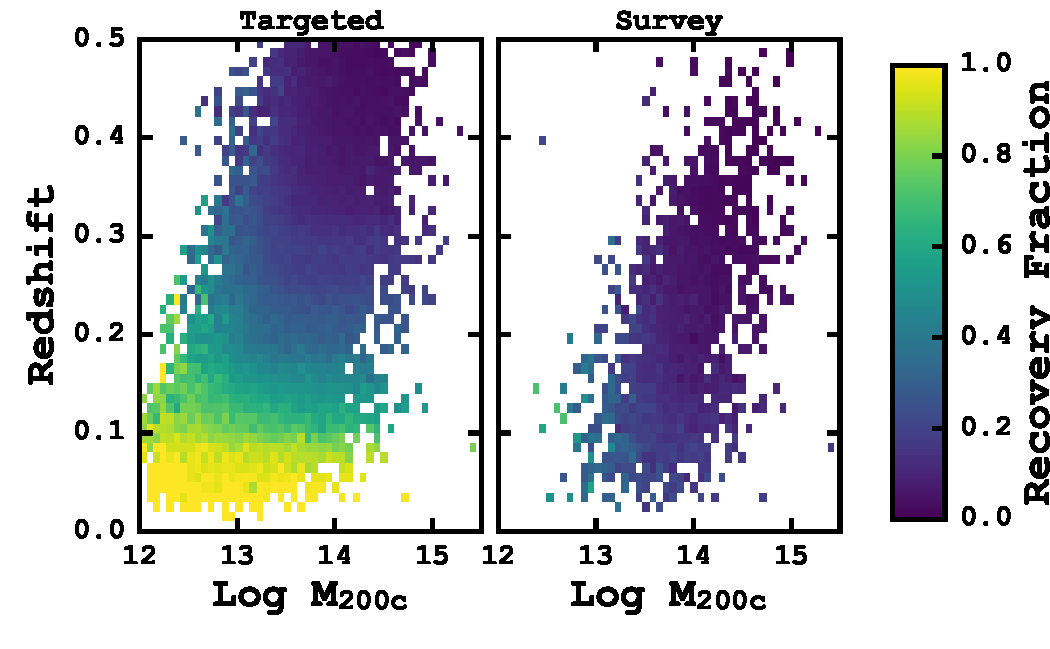
\includegraphics[width=0.8\textwidth]{figures1/recovery.pdf} 
	\caption{Recovery fractions ($N_{obs}/N_{True}$) of cluster member galaxies as a function of redshift and true cluster mass for the Targeted and Survey observing strategies. We have applied HETDEX-like observational limits on the cluster galaxy detection, and require at least five galaxies to be detected for a cluster to be recovered. The shading indicates the mean recovery fraction for clusters within each small bin of redshift and cluster mass. We find a significant decrease in the recovery of galaxies with increasing redshift. This leads to lower recovery fractions of high mass clusters as many only exist at larger redshifts. The significant decline in the number of galaxies observed with the Survey strategy is due to gaps in the VIRUS IFU, where the galaxies are missed.} \label{fig: recovery} 
\end{figure*}

As discussed in Section \ref{sec: observations}, the observational constraints place limits on the total number of clusters member galaxies expected to be recovered. Knowing these limits will provide important information for potential future follow up or Targeted observations. We recover 14,189 clusters with Targeted observations and 1,760 clusters with Survey observations, where we require a detection of $N_{obs} >=5$ galaxies for a cluster to be detected. Figure \ref{fig: recovery} shows the recovery fraction of member galaxies, the number of observed galaxies divided by the number of actual galaxies ($N_{obs}/N_{True}$), as a function of both redshift and cluster mass. As expected, the Targeted observing strategy where the individual clusters are targeted through several dithers to ensure near complete coverage, performs significantly better than the Survey observing strategy across all redshifts and cluster masses. With Perfect knowledge, recovery fraction would be unity across all redshifts and cluster masses where clusters exist.

For the Targeted observations, shown in the left panel of Figure~\ref{fig: recovery}, the pattern of decreasing recovery fraction as a function of redshift (y-direction) is due to the observational limits imposed. Because HETDEX is limited in apparent magnitude, we expect to recover fewer galaxies at higher redshift, where the galaxies are often below our $5\sigma$ detection threshold. For example, we tested this by constructing an artificial HETDEX-like survey, limited by volume for all galaxies with $M_g < -11$. In this case, our recovery fraction increases to $>70$\%, which shows that the flux limit is dominating the (lower) recovery of our flux-limited survey.

For the recovery fraction as a function of true cluster mass (x-direction), we find a general decrease in the recovery fraction of member galaxies with increasing cluster mass. This  is entirely a result of the flux limited survey (see previous paragraph). Because there are few high mass ($M_{200c}>5\times10^{14}$ \Msol) clusters, many of which are at moderately high redshift, the higher redshift cluster members suffer from the limiting apparent magnitude and suppress the recovery fraction at fixed mass. If we were to limit the Survey to $z<0.2$ we find the recovery fraction of clusters, across all masses, increases substantially, and we find a much more consistent detection fraction across all masses. 

For the Survey observations, the right panel of Figure~\ref{fig: recovery}, all of the same effects are at work. In addition we find that the fill factor, due to the gaps between the VIRUS IFUs, further reduces the number of cluster members detected. The median recovery fraction in Survey observations is almost exactly 4.5 times less than the Targeted median recovery fraction. As the total filling factor of the Survey observations increases the two lines will converge.

The recovery fractions in Figure~\ref{fig: recovery} are an outcome of the magnitude limit and \hbox{[\ion{O}{ii}]} line-flux limit of the survey. For Perfect observations, we would detect all members across all cluster masses and redshifts. Recovery fractions of clusters located a the low end of the redshift distribution will improve the most by follow-up targeted observations. But generally, the number of members observed (and subsequently more accurate cluster mass estimates) will benefit from follow-up observations regardless of the redshift. So follow-up observations should be tailored to the specific science goal.

\subsection{Mass estimates}
\begin{figure*} 
	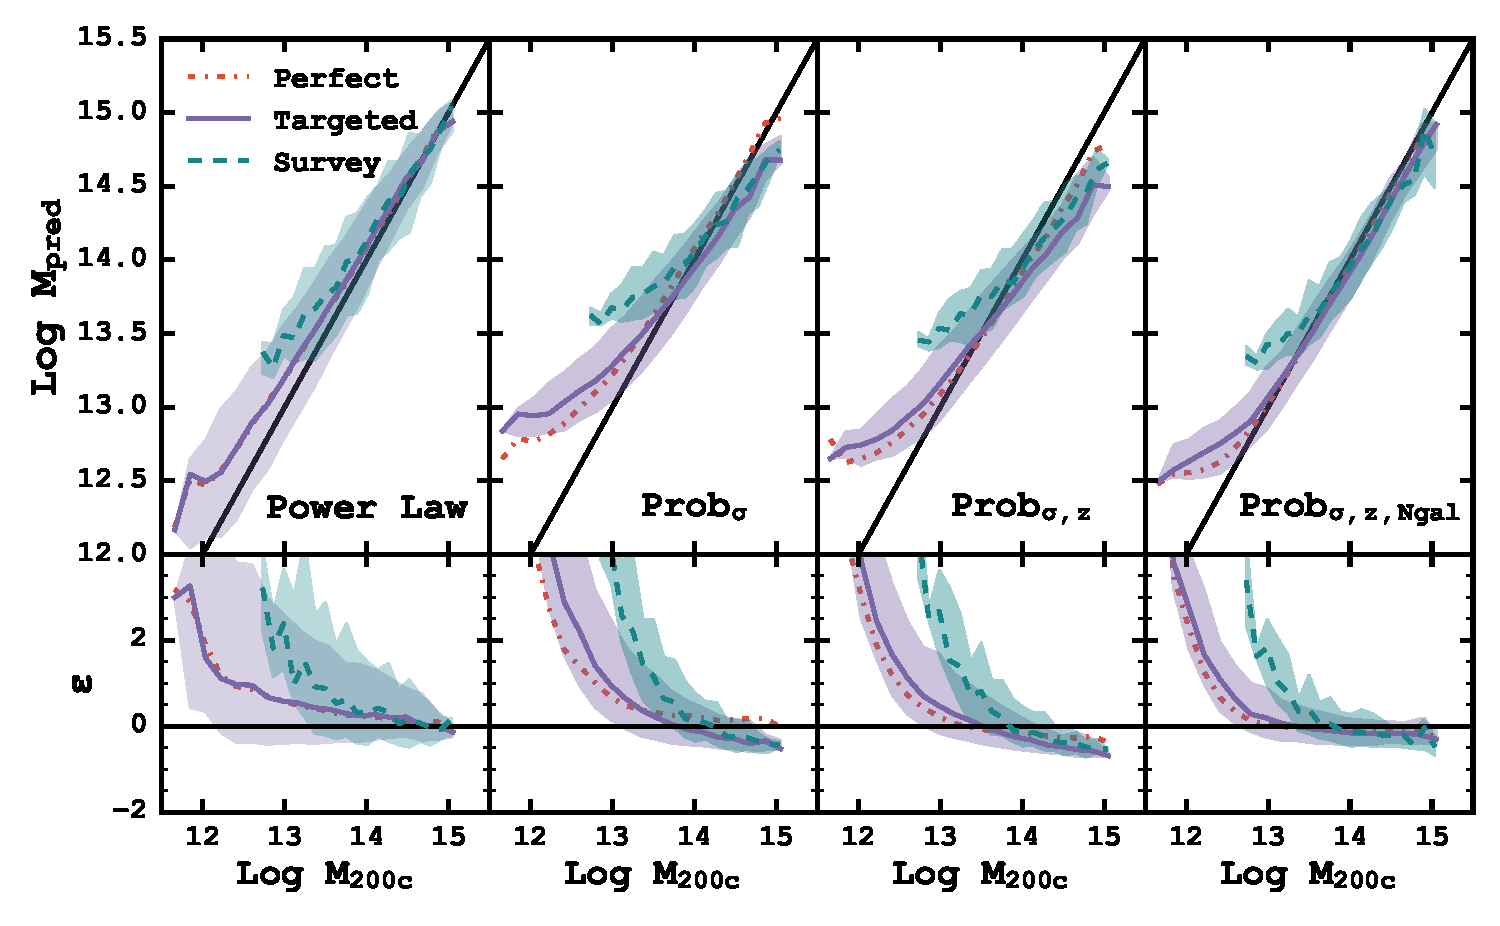
\includegraphics[width=\textwidth]{figures1/Probcomparison.pdf} 
	\caption{Mass predictions for the power law scaling relation (Equation~\ref{eq:power law}) and the probability based technique with different input features as a function of true cluster mass. The bottom row of panels shows the fractional error (Equation~\ref{eq: fractional error}) also as a function of true cluster mass. The solid black line shows the 1:1 relation, in both panels, between $M_{200c}$ and $M_{pred}$. The orange, dash-dotted line is the median predicted mass for perfect observations. The solid, purple line is the median predicted mass for the Targeted observing, and the green, dashed line is the median recovered mass for the HETDEX-like observations. The shaded regions represent the 68\% scatter around the median values.} \label{fig:Probability comparison} 
\end{figure*}

In this section we discuss the accuracy of the recovered masses compared to the true cluster mass from a set of observations. We report on three methods, the power law based approach (Eq. \ref{eq:power law}), the probability based approach (Section \ref{sec:probability method}) and the ML based method (Section \ref{sec:machine learning method}). For each method we consider observations with Perfect knowledge, Targeted observations and Survey observations. The cluster masses presented here are recovered using the best possible conditions, where we have perfect knowledge of the cluster membership. In reality, the mass recovery levels presented in this section represent an upper bound (the best) on the accuracy achievable through this method.

Because it represents the best possible scenario, the Perfect knowledge observations should serve as a baseline to compare the power law based, probability based and ML cluster mass recovery methods. And, while there are many possible metrics to evaluate performance, we compute two: the average bias (given in Table \ref{tbl:mass bias})
\begin{equation}\label{eqn: bias}
\mathrm{\mu_{bias}}(y,y_{pred}) = \frac{1}{N} \sum_{i=1}^N (y_{pred,i} - y_i).
\end{equation}
where $y$ are the true values and $y_{pred}$ are the predicted values, and the scatter about the bias (given in Table \ref{tbl:mass scatter})
\begin{equation}\label{eqn: scatter}
	\sigma_{bias}(y,y_{pred}, \mu_{bias}) = \bigg{[}\frac{1}{N-1} \sum_{i=1}^N (y_{pred,i} - y_i - \mu_{bias})^2 \bigg{]}^{1/2}
\end{equation}
with $N$ clusters in a given bin. Both metrics evaluate how closely the ensemble of predicted cluster masses are to the true cluster masses.

We begin with the Perfect knowledge observations. These observations are of the same clusters as the Targeted observations but without any observational limits. The cluster masses predicted by Equation \ref{eq:power law} gives the following results. For clusters with masses between Log M/\Msol $= 13 - 15.5$, we find $\mu_{bias} = 0.148\pm{0.008}$ dex and $\sigma_{bias} = 0.193\pm{0.001}$. The scatter in recovered masses can be attributed to both physical and numerical effects. The presence of any in-falling matter onto lower mass clusters can introduce a significant amount of substructure, leading to artificial biasing of the measured LOSVD to higher values, increasing the predicted mass \citeeg{Ntampaka2015}. Also, as the number of cluster galaxies decreases the LOSVD PDF is poorly sampled leading to poorly recovered cluster masses due to numerical effects. 

For the Targeted and Survey observations the power law predicted cluster masses give $\mu_{bias} =0.135\pm{0.003}$ dex, $\sigma_{bias} = 0.370\pm{0.002}$ and $\mu_{bias} =0.148\pm{0.008}$ dex, $\sigma_{bias} = 0.324\pm{0.006}$ , respectively. So for the clusters that we detect with Survey observations, we obtain similar levels of accuracy as to the Targeted observations, on the average. This does not mean that the Survey observations cannot be improved by Targeted observations. In fact, when comparing only the galaxies which overlap between the two samples the bias and scatter of the Targeted observations is significantly decreased as more cluster member galaxies are detected, better sampling the LOSVD PDF. The Targeted observations performs similarly on the average because many lower mass clusters are included in the sample, increasing the bias of the overall sample.

\begin{figure*} 
	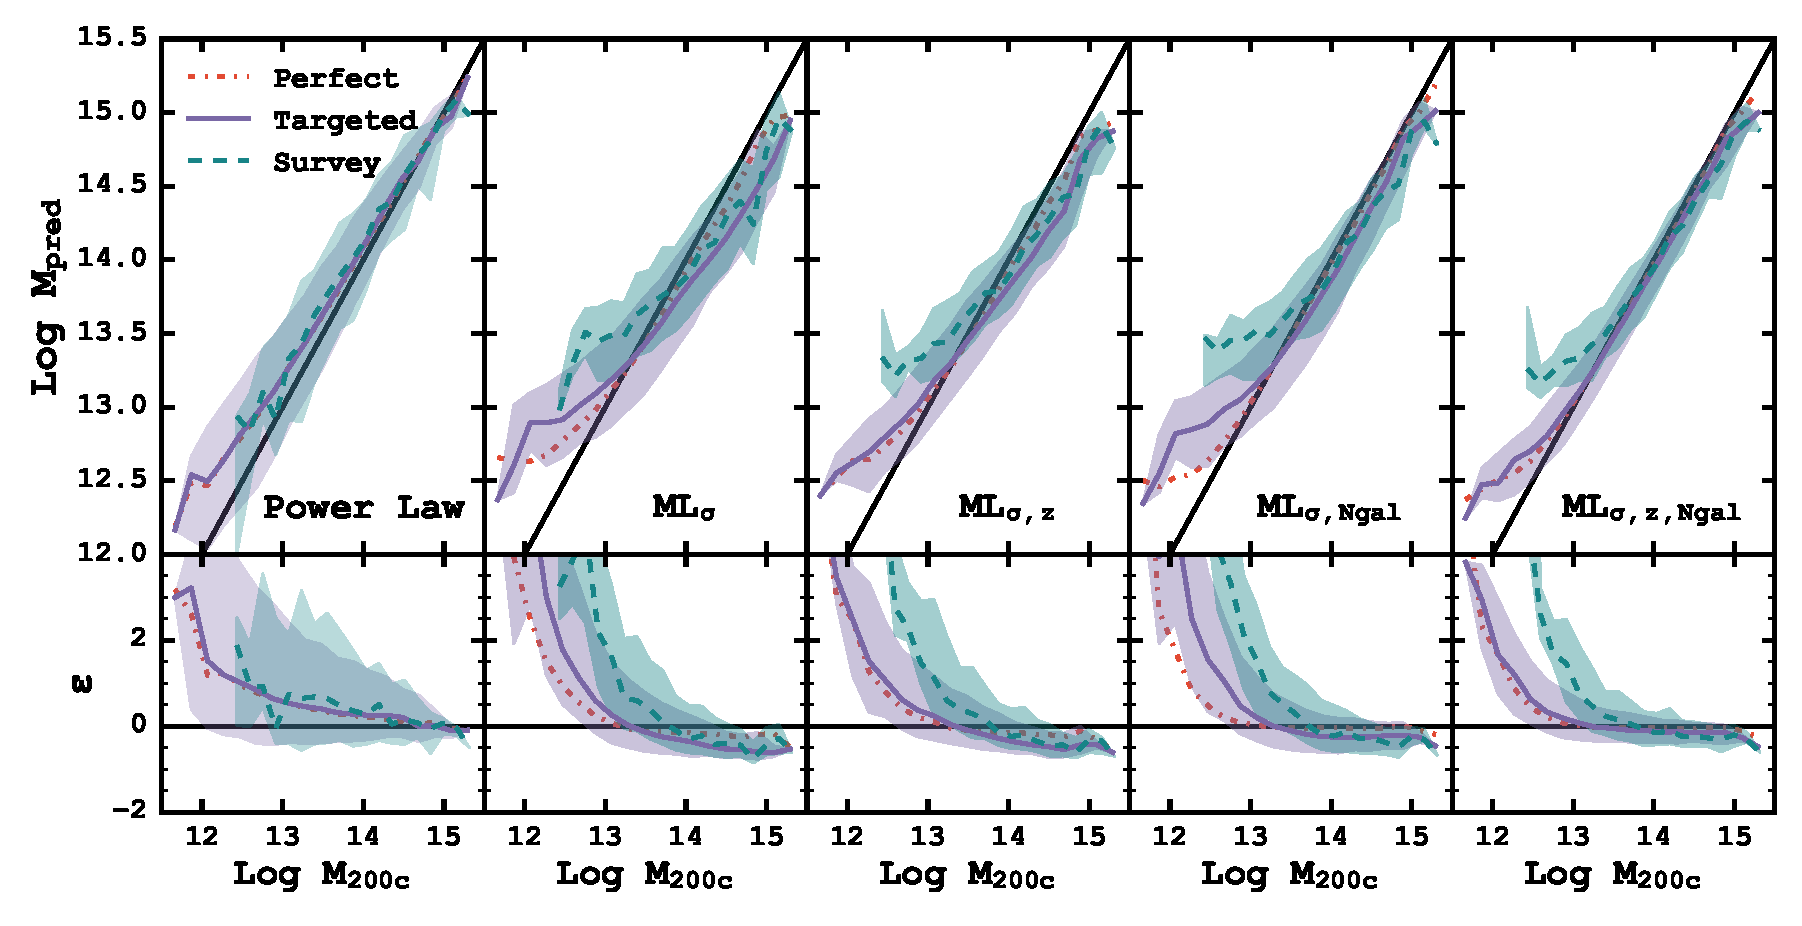
\includegraphics[width=\textwidth]{figures1/MLcomparison.pdf} 
	\caption{Mass predictions for the power law scaling relation (Equation~\ref{eq:power law}) and the ML based technique with different input features as a function of true cluster mass. The bottom row of panels shows the fractional error (Equation~\ref{eq: fractional error}) also as a function of true cluster mass. The solid black line shows the 1:1 relation. The orange, dash-dotted line is the median predicted mass for perfect observations. The solid, purple line is the median predicted mass for the Targeted observing, and the green, dashed line is the median recovered mass for the HETDEX-like observations. The shaded regions represent the 68\% scatter around the median values.} \label{fig: ML comparison} 
\end{figure*}

In both Figures \ref{fig:Probability comparison} and \ref{fig: ML comparison}, we show the predicted ($M_{pred}$) versus true ($M_{200c}$) cluster masses for each of the two observing strategries. The lower panels show the fractional cluster mass error defined as: 
\begin{equation}\label{eq: fractional error}
	\epsilon = (M_{pred} - M_{200c})/M_{200c}
\end{equation}
where $M_{pred}$ is the predicted cluster mass and $M_{200c}$ is the true cluster mass. Higher values of $\epsilon$ indicate the predicted cluster mass exceeds the true cluster mass.

Qualitatively, the top panels of Figures \ref{fig:Probability comparison} and \ref{fig: ML comparison} show that both the probability based and ML based methods out perform (closer to the black 1:1 relation) the power law method when taking advantage of other cluster observables ($z$, $N_{gal}$, etc.). Generally, we find that the single parameter probability and ML methods perform significantly poorer than the power law method, especially at low cluster masses. When combined with the cluster redshift, the predicted cluster masses are improved, because the range of cluster masses decrease with increasing redshift (see Figure~\ref{fig: recovery}). The final addition of the number of observed galaxies, $N_{gal}$ acts as a type of richness estimate, and significantly improves both the bias and the amount of scatter in the predicted masses.

\begin{landscape}
\begin{table}
\centering
\small
\caption{Mean bias (Eqn.~\ref{eqn: bias}) for different bins of predicted cluster mass. This table shows the bias in the predicted cluster mass for the perfect (top section), Targeted (middle section), and Survey (bottom section) observations in different predicted mass bins. The different mass recovery strategies are given in the leftmost column. It can be used to understand how the predicted cluster mass differs from the true cluster masses. Positive numbers indicate the predicted cluster mass over estimates when compared to the true cluster mass.}
\begin{tabular}{cccccccc} 
		&& \multic{6}{Bins -- Log $M_{pred}$} \\
		\cline{3-8} 
		\multicolumn{2}{c}{Method} & $12.5-13$ & $13-13.5$ & $13.5-14$ & $14-14.5$ & $14.5-15$ & $15-15.5$ \\
		\hline
		&& \multic{6}{Perfect Observations} \\
		\hline
		\multicolumn{2}{c}{Power Law} & $0.23\pm{0.007}$ & $0.16\pm{0.003}$ & $0.11\pm{0.002}$ & $0.07\pm{0.004}$ & $0.02\pm{0.011}$ & $-0.07\pm{0.045}$ \\
		\hline 
		\rottext{3}{Prob} &$\sigma$ & $0.32\pm{0.005}$ & $0.16\pm{0.003}$ & $0.10\pm{0.002}$ & $0.07\pm{0.004}$ & $0.05\pm{0.012}$ & $-0.18\pm{0.078}$ \\
		&$\sigma, z$ & $0.17\pm{0.005}$ & $0.01\pm{0.003}$ & $-0.06\pm{0.002}$ & $-0.11\pm{0.015}$ & $-0.14\pm{0.012}$ & $-0.38\pm{0.159}$ \\
		&$\sigma, z, N_{gal}$ & $0.04\pm{0.009}$ & $-0.02\pm{0.002}$ & $-0.02\pm{0.002}$ & $-0.05\pm{0.014}$ & $-0.22\pm{0.126}$ & \nd \\
		\hline
		\rottext{4}{ML} &$\sigma$ & $0.14\pm{0.006}$ & $-0.01\pm{0.003}$ & $-0.07\pm{0.003}$ & $-0.09\pm{0.005}$ & $-0.11\pm{0.014}$ & $-0.17\pm{0.090}$ \\
		&$\sigma, z$ & $0.12\pm{0.005}$ & $-0.01\pm{0.003}$ & $-0.06\pm{0.003}$ & $-0.08\pm{0.004}$ & $-0.11\pm{0.012}$ & $-0.24\pm{0.076}$ \\
		&$\sigma, N_{gal}$ & $0.04\pm{0.004}$ & $-0.02\pm{0.002}$ & $-0.02\pm{0.002}$ & $-0.02\pm{0.002}$ & $-0.02\pm{0.006}$ & $-0.08\pm{0.041}$ \\
		&$\sigma, z, N_{gal}$ & $0.04\pm{0.003}$ & $-0.02\pm{0.002}$ & $-0.02\pm{0.001}$ & $-0.02\pm{0.002}$ & $-0.02\pm{0.005}$ & $-0.08\pm{0.043}$ \\
		\hline
		
		&& \multic{6}{Targeted Observations} \\
		\hline
		\multicolumn{2}{c}{Power Law} & $0.20\pm{0.008}$ & $0.13\pm{0.005}$ & $0.10\pm{0.005}$ & $0.09\pm{0.007}$ & $0.02\pm{0.014}$ & $-0.08\pm{0.043}$ \\
		\hline
		\rottext{3}{Prob} &$\sigma$ & $0.40\pm{0.005}$ & $0.17\pm{0.003}$ & $0.02\pm{0.004}$ & $-0.08\pm{0.006}$ & $-0.19\pm{0.015}$ & $-0.35\pm{0.122}$ \\
		&$\sigma, z$ & $0.25\pm{0.005}$ & $0.08\pm{0.003}$ & $-0.06\pm{0.003}$ & $-0.21\pm{0.015}$ & $-0.35\pm{0.016}$ & $-0.59\pm{0.145}$ \\
		&$\sigma, z, N_{gal}$ & $0.13\pm{0.004}$ & $0.01\pm{0.003}$ & $-0.05\pm{0.003}$ & $-0.12\pm{0.018}$ & $-0.44\pm{0.177}$ & \nd \\
		\hline
		\rottext{4}{ML} &$\sigma$ & $0.26\pm{0.006}$ & $0.02\pm{0.004}$ & $-0.13\pm{0.005}$ & $-0.24\pm{0.008}$ & $-0.35\pm{0.022}$ & $-0.39\pm{0.054}$ \\
		&$\sigma, z$ & $0.18\pm{0.005}$ & $0.03\pm{0.003}$ & $-0.10\pm{0.004}$ & $-0.21\pm{0.006}$ & $-0.31\pm{0.021}$ & $-0.33\pm{0.063}$ \\
		&$\sigma, N_{gal}$ & $0.22\pm{0.005}$ & $0.00\pm{0.004}$ & $-0.13\pm{0.004}$ & $-0.16\pm{0.007}$ & $-0.13\pm{0.014}$ & $-0.19\pm{0.059}$ \\
		&$\sigma, z, N_{gal}$ & $0.09\pm{0.004}$ & $-0.01\pm{0.002}$ & $-0.05\pm{0.002}$ & $-0.08\pm{0.004}$ & $-0.08\pm{0.010}$ & $-0.19\pm{0.060}$ \\
		\hline
		
		&& \multic{6}{Survey Observations} \\
		\hline
		\multicolumn{2}{c}{Power Law} & $0.17\pm{0.068}$ & $0.17\pm{0.023}$ & $0.13\pm{0.014}$ & $0.07\pm{0.014}$ & $0.01\pm{0.022}$ & $-0.09\pm{0.062}$ \\
		\hline
		\rottext{3}{Prob} & $\sigma$ & $0.77\pm{0.030}$ & $0.42\pm{0.011}$ & $0.18\pm{0.008}$ & $-0.03\pm{0.009}$ & $-0.18\pm{0.017}$ & $-0.39\pm{0.102}$ \\
		&$\sigma, z$ & $0.61\pm{0.036}$ & $0.29\pm{0.012}$ & $0.08\pm{0.008}$ & $-0.11\pm{0.009}$ & $-0.38\pm{0.118}$ & $-0.48\pm{0.127}$ \\
		&$\sigma, z, N_{gal}$ & $0.48\pm{0.038}$ & $0.18\pm{0.011}$ & $0.02\pm{0.007}$ & $-0.08\pm{0.008}$ & $-0.50\pm{0.203}$ & \nd \\
		\hline
		\rottext{4}{ML} &$\sigma$ & $0.57\pm{0.046}$ & $0.24\pm{0.015}$ & $0.02\pm{0.012}$ & $-0.17\pm{0.013}$ & $-0.28\pm{0.027}$ & $-0.27\pm{0.117}$ \\
		&$\sigma, z$ & $0.48\pm{0.034}$ & $0.20\pm{0.013}$ & $0.03\pm{0.009}$ & $-0.13\pm{0.011}$ & $-0.26\pm{0.021}$ & $-0.31\pm{0.110}$ \\
		&$\sigma, N_{gal}$ & $0.55\pm{0.043}$ & $0.22\pm{0.013}$ & $0.00\pm{0.010}$ & $-0.14\pm{0.011}$ & $-0.22\pm{0.025}$ & $-0.19\pm{0.079}$ \\
		&$\sigma, z, N_{gal}$ & $0.42\pm{0.029}$ & $0.13\pm{0.011}$ & $-0.00\pm{0.007}$ & $-0.08\pm{0.008}$ & $-0.14\pm{0.016}$ & $-0.19\pm{0.079}$ \\
	\hline
	\end{tabular}
\label{tbl:mass bias}
\end{table}
\end{landscape}

We quantify the bias and scatter for all of the different cluster mass recovery strategies and observing methods in Table \ref{tbl:mass bias} and Table \ref{tbl:mass scatter}. It serves as a type of look up table for future cluster observations with HETDEX. The columns represent bins of predicted galaxy cluster mass and the individual values show the bias and scatter of the true cluster mass. The three horizontal sections represent Perfect, Targeted and Survey observations respectively. So, for example, if a cluster mass is predicted using the $\mathrm{ML}_{\sigma, z}$ method and Targeted observations to be Log M/\Msol\ $=13-13.5$, it is biased upward by $0.03\pm{0.003}$ dex and has a scatter of $0.24\pm0.009$ dex. 

\begin{table*}
\centering
\caption{Scatter (Eqn.~\ref{eqn: scatter}) in cluster mass after bias correction for different bins of predicted cluster mass. This table shows the scatter in the predicted cluster mass for the perfect (top section), Targeted (middle section), and Survey (bottom section) observations in different predicted mass bins. The different mass recovery strategies are given in the leftmost column. It can be used to understand how the predicted cluster mass differs from the true cluster masses.}
\begin{tabular}{cccccccc} 
		&& \multic{6}{Bins -- Log $M_{pred}$} \\
		\cline{3-8} 
		\multicolumn{2}{c}{Method} & $12.5-13$ & $13-13.5$ & $13.5-14$ & $14-14.5$ & $14.5-15$ & $15-15.5$ \\
		\hline 
		&& \multic{6}{Perfect Observations} \\
		\hline
		\multicolumn{2}{c}{Power Law} & $0.34\pm{0.005}$ & $0.22\pm{0.002}$ & $0.16\pm{0.002}$ & $0.14\pm{0.003}$ & $0.14\pm{0.008}$ & $0.11\pm{0.040}$ \\
		\hline 
		\rottext{3}{Prob} &$\sigma$ & $0.26\pm{0.004}$ & $0.20\pm{0.002}$ & $0.16\pm{0.002}$ & $0.14\pm{0.003}$ & $0.16\pm{0.009}$ & $0.19\pm{0.071}$ \\
		&$\sigma, z$ & $0.23\pm{0.003}$ & $0.19\pm{0.002}$ & $0.16\pm{0.002}$ & $0.55\pm{0.010}$ & $0.16\pm{0.009}$ & $0.39\pm{0.143}$ \\
		&$\sigma, z, N_{gal}$ & $0.47\pm{0.007}$ & $0.14\pm{0.001}$ & $0.10\pm{0.001}$ & $0.54\pm{0.010}$ & \nd & \nd \\
		\hline
		\rottext{4}{ML}	&$\sigma$ & $0.29\pm{0.004}$ & $0.24\pm{0.002}$ & $0.21\pm{0.002}$ & $0.19\pm{0.004}$ & $0.18\pm{0.010}$ & $0.22\pm{0.081}$ \\
		&$\sigma, z$ & $0.24\pm{0.003}$ & $0.20\pm{0.002}$ & $0.18\pm{0.002}$ & $0.16\pm{0.003}$ & $0.16\pm{0.009}$ & $0.19\pm{0.068}$ \\
		&$\sigma, N_{gal}$ & $0.19\pm{0.003}$ & $0.14\pm{0.001}$ & $0.10\pm{0.001}$ & $0.08\pm{0.002}$ & $0.07\pm{0.004}$ & $0.10\pm{0.037}$ \\
		&$\sigma, z, N_{gal}$ & $0.17\pm{0.002}$ & $0.13\pm{0.001}$ & $0.10\pm{0.001}$ & $0.07\pm{0.001}$ & $0.07\pm{0.004}$ & $0.11\pm{0.039}$ \\
		\hline
		
		&& \multic{6}{Targeted Observations} \\
		\hline
		 \multicolumn{2}{c}{Power Law} & $0.43\pm{0.006}$ & $0.39\pm{0.004}$ & $0.33\pm{0.004}$ & $0.27\pm{0.005}$ & $0.18\pm{0.010}$ & $0.11\pm{0.039}$ \\
		 \hline
		\rottext{3}{Prob} &$\sigma$ & $0.24\pm{0.003}$ & $0.25\pm{0.002}$ & $0.25\pm{0.003}$ & $0.22\pm{0.004}$ & $0.19\pm{0.011}$ & $0.30\pm{0.110}$ \\
		&$\sigma, z$ & $0.24\pm{0.003}$ & $0.24\pm{0.002}$ & $0.23\pm{0.002}$ & $0.56\pm{0.011}$ & $0.21\pm{0.012}$ & $0.36\pm{0.131}$ \\
		&$\sigma, z, N_{gal}$ & $0.20\pm{0.003}$ & $0.19\pm{0.002}$ & $0.17\pm{0.002}$ & $0.67\pm{0.013}$ & \nd & \nd \\
		\hline
		\rottext{4}{ML} &$\sigma$ & $0.30\pm{0.004}$ & $0.32\pm{0.003}$ & $0.32\pm{0.003}$ & $0.30\pm{0.006}$ & $0.29\pm{0.016}$ & $0.13\pm{0.049}$ \\
		&$\sigma, z$ & $0.26\pm{0.004}$ & $0.25\pm{0.002}$ & $0.24\pm{0.003}$ & $0.23\pm{0.004}$ & $0.27\pm{0.015}$ & $0.16\pm{0.057}$ \\
		&$\sigma, N_{gal}$ & $0.27\pm{0.004}$ & $0.27\pm{0.003}$ & $0.27\pm{0.003}$ & $0.25\pm{0.005}$ & $0.18\pm{0.010}$ & $0.15\pm{0.053}$ \\
		&$\sigma, z, N_{gal}$ & $0.21\pm{0.003}$ & $0.18\pm{0.002}$ & $0.16\pm{0.002}$ & $0.14\pm{0.003}$ & $0.12\pm{0.007}$ & $0.15\pm{0.054}$ \\
		\hline
		
		&& \multic{6}{Survey Observations} \\
		\hline
		\multicolumn{2}{c}{Power Law} &$0.40\pm{0.050}$ & $0.41\pm{0.016}$ & $0.38\pm{0.010}$ & $0.32\pm{0.010}$ & $0.25\pm{0.016}$ & $0.15\pm{0.056}$ \\
		\hline
		\rottext{3}{Prob} &$\sigma$ & $0.11\pm{0.024}$ & $0.18\pm{0.008}$ & $0.22\pm{0.006}$ & $0.22\pm{0.007}$ & $0.19\pm{0.012}$ & $0.25\pm{0.092}$ \\
		&$\sigma, z$ & $0.13\pm{0.028}$ & $0.19\pm{0.008}$ & $0.22\pm{0.006}$ & $0.21\pm{0.007}$ & $1.31\pm{0.084}$ & $0.32\pm{0.115}$ \\
		&$\sigma, z, N_{gal}$ & $0.14\pm{0.030}$ & $0.18\pm{0.008}$ & $0.19\pm{0.005}$ & $0.19\pm{0.006}$ & \nd & \nd \\
		\hline
		\rottext{4}{ML} &$\sigma$ & $0.27\pm{0.034}$ & $0.27\pm{0.011}$ & $0.31\pm{0.008}$ & $0.30\pm{0.009}$ & $0.30\pm{0.019}$ & $0.29\pm{0.106}$ \\
		&$\sigma, z$ & $0.20\pm{0.025}$ & $0.24\pm{0.009}$ & $0.24\pm{0.006}$ & $0.25\pm{0.008}$ & $0.24\pm{0.015}$ & $0.27\pm{0.100}$ \\
		&$\sigma, N_{gal}$ & $0.25\pm{0.032}$ & $0.23\pm{0.009}$ & $0.27\pm{0.007}$ & $0.26\pm{0.008}$ & $0.27\pm{0.018}$ & $0.20\pm{0.072}$ \\
		&$\sigma, z, N_{gal}$ & $0.17\pm{0.021}$ & $0.21\pm{0.008}$ & $0.20\pm{0.005}$ & $0.19\pm{0.006}$ & $0.17\pm{0.011}$ & $0.20\pm{0.071}$ \\
		 \hline
	\end{tabular}
\label{tbl:mass scatter}
\end{table*}

A few caveats apply to the numbers given in Table \ref{tbl:mass bias} and Table \ref{tbl:mass scatter}. While we provide corrections for cluster masses above $10^{15}$ \msol, they are estimated from only a handful of objects, and do not constitute a representative sample of clusters. This becomes particularly apparent for the probability methods with many features. As the number of observed features increases, the number of training clusters in any particular bin decreases. This leads to highly skewed biases and scatters for the high mass clusters and probability methods. We do not report any bin where such small number statistics dominate in Tables~\ref{tbl:mass bias} and \ref{tbl:mass scatter}. On the opposite end of the cluster mass spectrum, there are very few, if any, clusters detected with Targeted or Survey observations below $5\times10^{12}$ \msol. Therefore, while we show these points in Figures~\ref{fig:Probability comparison} and \ref{fig: ML comparison}, we exclude their biases and scatters from Tables~\ref{tbl:mass bias} and \ref{tbl:mass scatter} for the same reasons. 
 
The method which produce the lowest scatter and bias depends on the mass of the cluster in question and the type of observations used. For the Targeted observations, the power law method outperforms all other methods, in terms of bias and scatter, for the highest mass clusters. But outside of the two highest mass bins, the $\mathrm{ML}_{\sigma, z, N_{gal}}$ method shows the smallest amount of scatter and bias most consistently. With Survey observations, the power law again provides the lowest bias in the highest cluster mass bins, but is outperformed in terms of scatter by the other two methods. The $\mathrm{ML}_{\sigma, z, N_{gal}}$ method shows the smallest amount of scatter and bias most consistently across the cluster mass range in question.
 
\subsection{Impact of Training Sample Cosmology}
All simulations (including that used for Buzzard) use specific values for cosmological parameters. When using simulation data to train ML methods, we incorporate all of those assumptions into the learned feature associations. One could imagine that the specific values of the cosmological parameters in the training sample could bias the ML results when applied to data (real or simulated) created from an unknown true set of cosmological parameters. 

To test for this, we used the Millennium simulation as an alternative data set. The Millennium simulation uses a set of cosmological parameters that are substantially different from Buzzard. The Millennium simulation adopts a flat cosmological model based of the values derived from the Two-degree Field Galaxy Redshift Survey \citep{Colless2001} and the first year data of the \emph{Wilkinson Microwave Anisotropy Probe} (WMAP; \citealt{Spergel2003}): $\Omega_\Lambda = 0.75$, $\Omega_M = 0.25$, $\sigma_8 = 0.9$, $n_s = 1$ and $H_0= 73$ \kms \mpc. The clusters in Millennium provide a testing sample to understand how a training sample derived from Buzzard will impact the mass recovery on a wholly new dataset. 

We repeat our analysis using cluster halo and galaxy catalogs from the Millennium simulation \citep{Springel2005a} obtained via querying the Millennium online database\footnote{http://gavo.mpa-garching.mpg.de/Millennium/} \citep{Lemson2006}. The Millennium simulation tracks $2160^3$ dark matter particles of $8.6\times 10^8 ~h^{-1}$ \Msol\ inside a comoving 500 $(h^{-1} \mathrm{Mpc})^3$ box from $z=127$ to 0. 

We select 4,806 clusters, comprised of 623,663 galaxies, at $0.02 < z < 0.5$ and $M > 10^{13}$ \Msol, and apply the same data processing as with the Buzzard galaxies. We begin by assigning each galaxy an \hbox{[\ion{O}{ii}]} flux value (see Section \ref{sec: oii luminosity}), and ``observe'' each galaxy using realistic (see Section \ref{sec: observations}) observational limits. After recovering 3750 clusters which have at least five galaxies observed, we calculate the LOSVD of each cluster as in Section \ref{sec: LOSVD}. 

\begin{figure} 
	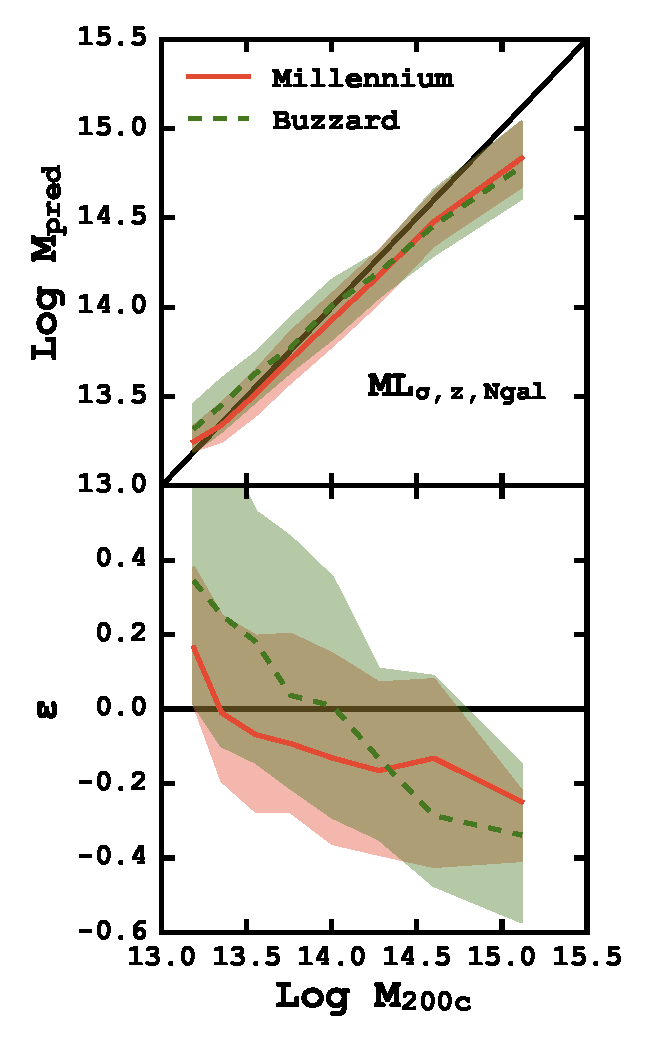
\includegraphics[width=\textwidth]{figures1/millBuzzComparison.pdf} 
	\caption{\emph{Top:} ML based cluster mass predictions for the Millennium simulation clusters where the ML method has been trained with either a subset of the Millennium clusters (solid line) or the Buzzard catalog (dashed line). The shaded areas show the 68\% scatter around the median. The solid black line shows the 1:1 relation. \emph{Bottom:} The fractional error (Equation~\ref{eq: fractional error}) also as a function of true cluster mass. The similarity of the predictions with the different training sets demonstrates how the ML method is not sensitive to the underlying cosmological assumptions.} \label{fig: mill buzz comparison} 
\end{figure}

We conduct our test in two ways. Both use the ML methods (see Section \ref{sec:machine learning method}) to predict the cluster masses of the Millennium clusters, but each test uses a different training set. First, we use the full set of clusters detected in the Buzzard catalogs (14,000 clusters with $M > 10^{11}$ \msol) to train the ML. Second, the Millennium clusters are split into training-testing samples. This provides a test case where we have different cosmological choices between the training and testing samples, and the same cosmological assumptions in both samples. 

The top panel of Figure~\ref{fig: mill buzz comparison} shows the ML predicted cluster masses for the $\sim$4000 Millennium clusters as a function of true cluster mass. The orange (Millennium) and green (Buzzard) colors indicate the two different training samples. The median (solid and dashed lines) predicted cluster masses show similar trends regardless of the training data set used. The bottom panel of Figure~\ref{fig: mill buzz comparison} shows the fraction error (Equation~\ref{eq: fractional error}) also as a function of true cluster mass. The large amount of scatter (the shaded area) in the fractional error for the Buzzard-trained predictions is due to the training set including clusters with masses below the $M = 10^{13}$ \Msol\ threshold for the Millennium clusters. This allows the ML method to predict masses which can be significantly different, whereas the Millennium training set does not include $M < 10^{13}$ \Msol\ clusters, which reduces the scatter of the predicted masses.

Based on these tests, we do not find a significant cause for concern with using trained ML methods to predict our galaxy cluster masses when the underlying cosmological choices are different. This highlights the versatility of our chosen ML method. The ML method could be further diversified by including cluster measurements from a wide range of cosmological simulations (or observations) which, in affect, marginalizes over all the cosmological assumptions further reducing the dependence.

\section{HETDEX as a Galaxy Cluster Survey at $z < 0.5$}\label{sec:discussion}

\subsection{Constraints on Cosmological Parameters}
Galaxy clusters trace the peaks in the universal matter density, often referred to as the power spectrum of matter density fluctuations or the matter power spectrum. This enables them to be sensitive probes of $\Omega_m$, the total mass ($\Omega_b + \Omega_c$) density, and $\sigma_8h^{-1}$, the normalization of the power spectrum. We constrain these parameters by the comparison of the number density of observed clusters to that predicted in cosmological models. Although, in reality, one measures $\sigma_8h^{-1}\Omega_m^q$, where the value of $q$ depends on the masses and redshifts of the halos considered.

To get a sense of how well HETDEX will be able to constrain cosmological parameters we follow the discussion of \defcitealias{Weinberg2013}{W13}\cite{Weinberg2013} (hereafter \citetalias{Weinberg2013}), and begin with a few simplifying assumptions. While sensitive to $\Omega_m$, the number density of clusters does not necessarily provide the strongest contraint, but combined with other data sets (\eg, CMB, BAO, supernovae, WL, etc.) it will constrain $\Omega_m$ to higher precision.

To estimate the error associated with a measurement of $\sigma_8h^{-1}$ (which \citetalias{Weinberg2013} refer to as $\sigma_{11,abs}$), \citetalias{Weinberg2013} consider two sources of uncertainty, the systematic uncertainties in cluster mass calibration and the statistical uncertainty in the observed number density of clusters. The authors combine these two uncertainties though (their Eq. 141):
\begin{equation}
\Delta \ln \sigma_8h^{-1}(z) \approx q(z)\times 
        \max\left[ \Delta \ln M, \alpha(z)^{-1} \Delta \ln N \right].
\label{eq:sigElapprox}
\end{equation}
where $q$ is the degeneracy exponent between $\sigma_8h^{-1}$ and $\Omega_m$, $\Delta \ln M$ is the mass scale uncertainty, $\Delta \ln N$ is the cluster statistical uncertainty, and $\alpha$ is slope of the cumulative HMF. Using the \cite{Tinker2008} HMF at $z\sim0.2$ and a limiting cluster mass of $10^{14}$ \Msol, \citetalias{Weinberg2013} estimate $q\sim0.4$, $\alpha\sim3$, and find that any cluster survey with more than 10-20 clusters is dominated by the uncertainty in the overall mass scale.

For a survey such as HETDEX, we can estimate the constraints on $\sigma_8h^{-1}$ using Equation \ref{eq:sigElapprox}. If we consider clusters with masses above $10^{14}$ \Msol\ and with Perfect knowledge observations, the lowest mass scale uncertainty (given in Table~\ref{tbl:mass scatter}) is $\Delta_{log_{10}}M \sim 0.075$ dex or about 20\%. This gives a uncertainty on $\sigma_8h^{-1}$ of 7\%. For clusters above $10^{14}$ \Msol, Survey observations constrain the masses to about 51\% which, in turn, constrains $\sigma_8h^{-1}$ to 20\%.

Because of the simplifying assumptions, and the superior quality of the data (no contamination, signal-to-noise issues, etc.), realistic expectations for HETDEX is to directly constrain $\sigma_8h^{-1}$ is not yet competitive with other methods (\eg, CMB, WL, X-ray). For example, \cite{deHaan2016} constrain $\sigma_8h^{-1}$ to $\sim5$\% using a sample of 337 SZE detected clusters from the SPT-SZE survey. For the $\sim1500$ clusters detected with Survey observations to constrain $\sigma_8h^{-1}$ and to be dominated by cluster statistics alone ($\Delta \ln N \sim N^{-1/2}$), the absolute cluster calibration would need to be better than 2.5\%. For a fully Targeted survey, about 14,000 clusters, this cluster mass calibration uncertainty reduces to $>1\%$. So while, the contraints produced by HETDEX will be larger than some other studies, the type of data provided by HETDEX will enable an independent calibration from other cluster mass measurements. This will provide important systematics checks on other studies and will ultimately improve the measurements of $\sigma_8h^{-1}$ .

\subsection{Scale and Scatter of the Richness-Cluster Mass Relation}
Large-scale optical surveys (\eg, DES and LSST) expect to detect hundreds of thousands of galaxy clusters at $z < 1$. Because they produce photometry only, a major challenge for these surveys is relating a cluster observable to the total DM mass. One promising cluster mass estimator is the optical richness \citeeg{Abell1958}. Specifically, here, we use $\lambda$, the weighted number of galaxies within a scale aperture \citeeg{Rozo2011} as calculated by the redMapper algorithm \citep{Rykoff2012}. Previous works \citeeg{Rozo2010} show that the richness correlates strongly with cluster mass on the average, but the absolute mass scale of the optical richness mass estimator and the scatter in cluster mass at fixed optical richness are imprecisely known \citep{Rykoff2012}. These systematics remain the major source of uncertainty in deriving cosmological constraints from cluster abundances and must be measured using independent methods to realize the full potential of these types of surveys.

One of the main goals of this study is to understand how well HETDEX will be able to measure the scatter in the richness-mass relationship. To this end, we choose to impose a richness-mass relation onto the clusters in the Buzzard catalogs. The true richness-mass relation could depend strongly on the number and types of environmental effects, because such effects have a strong impact on the number and types of galaxies observed in clusters \citeeg{Gunn1972,Balogh2000,White2010}. Any environmental effects included in Buzzard could potentially impact our observed richness. The imposition of an empirical richness-mass relation ensures the richness values correspond correctly to the clusters in our sample, could provide direct observational tests in the future.

We generate richnesses based on the true cluster masses, and for testing, we assume two versions of the richness-mass relationship. \cite{Farahi2016} base the relation on stacked velocity dispersions, and \cite{Simet2016} use weak lensing measurements to construct their relation. Because we are investigating HETDEX's ability to recover the overall cluster mass scale and underlying scatter in the mass-richness relationship, we use the true cluster masses perturbed by a known amount to estimate the observed richness. 

To confirm that measuring the underlying scatter is possible, after generating richness values we calculate the scatter of the cluster masses at fixed $\lambda$, $\sigma_{M|\lambda}$, by comparing the true, unperturbed cluster masses against the richness. We do recover the expected scatter, often, to well within 0.01 dex. We repeat the process with both assumed richness-mass relationships and recover the expected scatter in both instances. 

We use the lambda values generated above in combination with the $\mathrm{M}_{\sigma,z,N_{gal}}$ predicted cluster mass which have been bias corrected using the values in Table~\ref{tbl:mass bias} and denoted $\mathrm{M_{pred,corr}}$. The use of biased cluster mass predictions inhibits our ability to accurately recover any scatter in richness-mass relationship, and is discussed further below. 

Primarily, we are interested in the intrinsic scatter of the richness-mass relationship. This is because HETDEX is uniquely situated to estimate the scatter, whereas studies relying on stacked data \citeeg{Farahi2016,Simet2016} lose that information. We begin by attempting to constrain the absolute mass scale, and as part of our fitting process, we estimate the overall scatter in the relationship. In order to understand how HETDEX will constrain the absolute mass scale, we find the best fitting relation to our richness-mass data. To generate the best fitting lines, we follow the general procedure of \cite{Hogg2010}, by defining an objective function and then minimizing the loss. Our objective function is
\begin{equation}\label{eq:objectivei}
P(y_i|x_i,\sigma_{yi},m,b,\sigma) = \frac{1}{\sqrt{2\,\pi\,(\sigma_{yi}^2+\sigma^2)}}
 \,\exp\left(-\frac{[y_i - m\,x_i - b]^2}{2\,(\sigma_{yi}^2+\sigma^2)}\right)
\end{equation}
where $y_i$ is the observed cluster mass, $x_i$ is the observed richness, $\sigma_{yi}$ is the uncertainty in observed cluster mass, $m$ is the power law slope, $b$ is the overall cluster mass scale, and $\sigma$ is the intrinsic scatter between richness and cluster mass. We assume that the intrinsic scatter is constant from point to point and that all of the measurement errors are Gaussian. We convert this objective function into a likelihood by taking the product of all the individual probabilities:  
\begin{equation}\label{eq:like}
\mathscr{L} = \prod_{i=1}^N \ P(y_i|x_i,\sigma_{yi},m,b, \sigma).
\end{equation}
We again rely on MCMC samples to sample the posterior probability distribution and thus maximize the likelihood. The best fitting slope and intercept are quoted as the median value of the posterior probability distribution with 68\% error bars defined as the square root of the second moment of the same distribution.

We limit our clusters to those with $10 \leq \lambda < 130$ in our fitting analysis because above $\lambda=130$ there are too few clusters and number-counting errors dominate. Other observational studies \citeeg{Saro2015} which have lower limits on $\lambda$, so we exclude anything less than $\lambda=10$. For a richness-mass relation with an intrinsic scatter of $\langle \sigma_{M|\lambda} \rangle = 0.25$ dex, we find a best-fitting relation for the Targeted observations as
\begin{equation}
	\mathrm{Log}\ M_{200c}/\Msol = 12.46\pm0.02 + 1.07\pm0.02\ \mathrm{Log}\ \lambda
\end{equation} 
and the Survey observations as
\begin{equation}
	\mathrm{Log}\ M_{200c}/\Msol = 12.64\pm0.05 + 0.98\pm0.03\ \mathrm{Log}\ \lambda
\end{equation} 
This gives $M_{200c} = (1.45\pm0.12)\times10^{14}$ \Msol\ and $M_{200c} = (1.59\pm0.27)\times10^{14}$ \Msol\ at $\lambda=40$ for the Targeted and Survey observations respectively. In both cases, this normalization differs significantly from the $M_{200c} \approx 2.1\times10^{14} h^{-1}$ \Msol\ found in recent work \cite{Li2016, Simet2016}. If the intrinsic scatter is reduced to $\sim 0.05$ dex we recover an overall normalization of $M_{200c} = (2.14\pm0.12)\times10^{14}$ \Msol\ and $M_{200c} = (2.10\pm0.26)\times10^{14}$ for the Targeted and Survey observations at $\lambda=40$.

We also estimate the intrinsic scatter. For observations with a richness-mass relation intrinsic scatter of $\langle \sigma_{M|\lambda} \rangle = 0.25$ dex, we recover $\langle \sigma_{M|\lambda} \rangle = 0.236\pm0.003$ dex and $\langle \sigma_{M|\lambda} \rangle = 0.257\pm0.007$ dex for the Targeted and Survey observations respectively. 

%The discrepancy between the intrinsic value and the measured value is due to the uncertainties in the individual cluster mass predictions. As the prediction intervals are narrowed, the recovered intrinsic scatter approaches the true value. For example, with cluster mass prediction intervals half the size of the current intervals we measure $\langle \sigma_{M|\lambda} \rangle$ to be $\sim 0.25$ and $\sim 0.23$ dex for the two sets of observations.

\begin{figure} 
	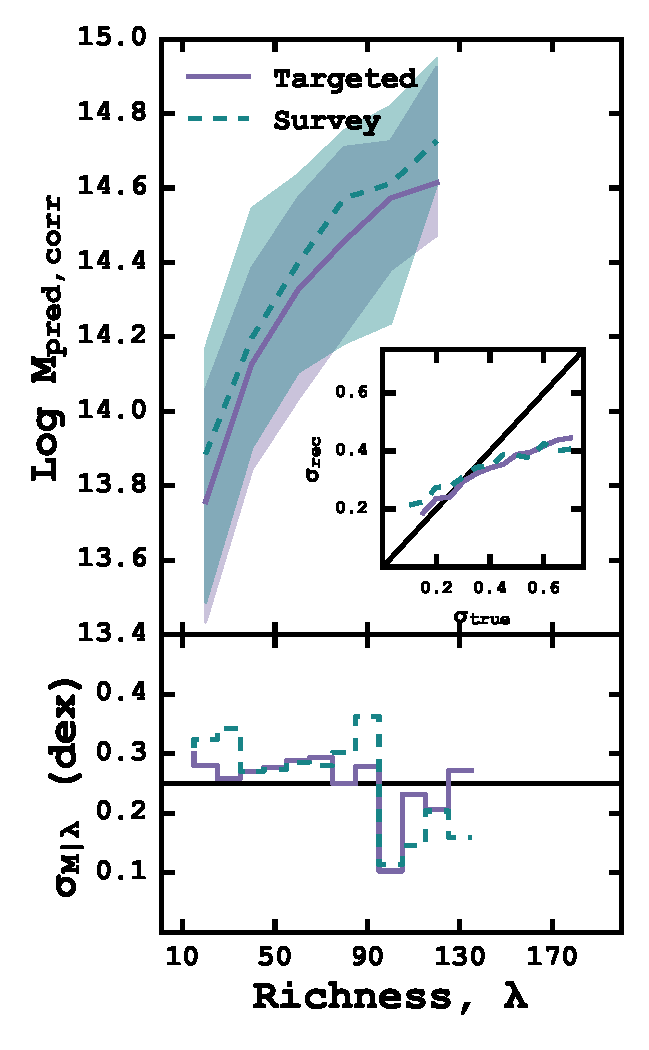
\includegraphics[width=\textwidth]{figures1/massRichness.pdf} 
	\caption{\emph{Top}: The optical richness, $\lambda$, versus the corrected predicted cluster mass. The solid, purple line is the median predicted mass for the Targeted observing, and the turquoise, dashed line is the median recovered mass for the HETDEX-like observations. The shaded regions represent the 68\% scatter around the median values. \emph{Bottom}: The scatter in the relation at fixed richness. The solid black line shows the intrinsic scatter of $\sigma_{true}=0.25$ dex. Color coding is the same as the top panel. \emph{Inset}: The evolution of the intrinsic scatter versus the average recovered scatter, $\sigma_{rec}$.} \label{fig:mass richness} 
\end{figure}

Figure \ref{fig:mass richness} summarizes the main results of this investigation. The top panel shows the generated optical richness, $\lambda$, versus the predicted cluster mass. The cluster masses are the $\mathrm{ML}_{\sigma, z, N_{gal}}$ based and correspond to the Targeted and Survey observation strategies. The bottom panel of Figure \ref{fig:mass richness} shows the scatter in the predicted cluster masses at fixed richness, $\sigma_{M|\lambda}$. The solid line represents the intrinsic amount of scatter added to the masses. The cluster masses are binned in increasing ten richness intervals ($10-20$, $20-30$, etc.). The inset upper panel shows the intrinsic scatter versus the recovered average scatter at fixed richness, $\langle \sigma_{M|\lambda} \rangle$ and illustrates how well the two observation strategies recover the intrinsic scatter. 

We find that we are able to accurately recover an average intrinsic scatter of $0.2 <\langle \sigma_{M|\lambda} \rangle <0.3$ dex, finding $\langle \sigma_{M|\lambda} \rangle = 0.257\pm0.007$ at $\sigma_{true} = 0.25$ with Survey observations. This is very promising as other observational studies have estimated the intrinsic scatter of real clusters to be $\sim0.25$ dex \citeeg{Rozo2014, Rozo2015}. As the intrinsic scatter increases or decreases, we fail to recover the scatter as accurately.

For the richness range $10 \leq \lambda < 130$ the intrinsic scatter in between the $\mathrm{M_{pred,corr}}$ predicted cluster masses and the true cluster mass (the basis of our richnesses) is $\sim0.15$ dex for Targeted observations and $\sim0.20$ dex for Survey observations. This forms an effective floor on the amount of scatter we are able to recover from our fitting process. As we reduce the overall scatter in our cluster mass recovery, this floor will lower. We underestimate the scatter in high intrinsic scatter relations because any residual bias remaining in the predicted clusters masses after correction reduces the observed scatter. Because the bias subtraction when creating $\mathrm{M_{pred,corr}}$ subtracts the mean bias, we are left with a small amount of residual bias, lowering the measured scatter for high scatter relationships.

\section{Summary}\label{sec:summary}
Here, we present detailed simulations of the upcoming HETDEX survey's applicability to the detection and total mass measurement of galaxy clusters. Using mock galaxy catalogs and HETDEX-like observational strategies and limits, we observe our simulated sky, estimate the number of clusters observed, and derive basic cluster parameters, redshift, line-of-sight velocity dispersion (LOSVD). Using a traditional power law-based, velocity dispersion, scaling relation along with more advanced probability and machine learning (ML) techniques, we estimate each cluster's total mass. We discuss each cluster mass estimate's precision, and discuss HETDEX's ability to constrain the cosmological parameter $\sigma_8 h^{-1}$ based on those predicted cluster masses. In addition, we comment on how HETDEX may improve current and future photometric large-area sky surveys' cluster mass estimates derived from optical richness.

Our main conclusions are the following:
\begin{enumerate}
	\item After considering HETDEX's observational limits, we find 14,189 clusters with at least five cluster members in the HETDEX survey volume. Of those, 1,760 clusters are detected with HETDEX-like survey observations. The number of cluster members recovered with Survey observations is almost exactly 4.5 times fewer than a fully Targeted survey, across both a wide range of redshifts and cluster masses.
	
	\item We find a traditional power law conversion from LOSVD to cluster mass predicts the true cluster mass with little bias or scatter for clusters Log M/\Msol\ $=14.5$ and above. Below this mass the bias and scatter rapidly increases. In contrast, the probability based and ML based cluster mass estimators are able to predict cluster mass with similar or smaller scatter across all cluster masses. The scatter further decreases when the probability based and ML estimators are combined with other cluster observables besides the LOSVD. For HETDEX-like observations and clusters with $13 < \mathrm{Log}\, M/\Msol <14.5$, we find the $\mathrm{ML}_{\sigma, z, N_{gal}}$ method results in the smallest scatter. Below Log M/\Msol\ $=13$ no method with Survey observations gives a bias of less than 50\%. For the highest mass clusters the power law method gives the lowest bias and scatter. In short, no single method is superior in all regards. The technique should be chosen to minimize the desired systematic, but we find $\mathrm{ML}_{\sigma, z, N_{gal}}$ provides the best performance across the large range of cluster masses, and observation strategies.
	
	\item In general, we find that the measured scatter of cluster masses decreases when considering Targeted versus Survey observations. Clusters at all masses can benefit from targeted follow-up observations, although the accuracy gain will be smaller than can be achieved from cluster mass prediction method changes. Targeted follow-up observations reduces the measured scatter by $\sim10\%$ when comparing like recovery methods.
	
	\item The $\sim51\%$ cluster mass accuracy of Survey observations places approximately a 20\% constraint on $\sigma_8 h^{-1}$. This can be tightened to approximately 12\% with follow-up targeted observations. Most importantly, the observations from HETDEX will provide systematics checks on other studies, ultimately improving all future measurements of $\sigma_8 h^{-1}$
	
	\item HETDEX will be able to place important, independent constraints on the amount of scatter in the optical richness-mass relationship. It will to a less extent constrain the overall normalization of the relation. This should provide an important tool in the calibration of large-area sky surveys which rely on photometric data only to estimate cluster masses.
\end{enumerate}

It is the author's hope that this work may be useful to others when conducting their own research. Because this work relies heavily on (often) complex data analysis, and in order to promote transparency and reproducible science, we provide all of the code used to conduct this study at https://github.com/boada/desCluster. Regrettably, large file size prevents including the source data with the analysis routines. The authors are happy to provide them, if requested.

 
%%%%%%%%%%%%%%%%%%%%%%%%%%%%%%%%%%%%%%%%%%%%%%%%%%%
%
%  New template code for TAMU Theses and Dissertations starting Fall 2012.  
%  For more info about this template or the 
%  TAMU LaTeX User's Group, see http://www.howdy.me/.
%
%  Author: Wendy Lynn Turner 
%	 Version 1.0 
%  Last updated 8/5/2012
%
%%%%%%%%%%%%%%%%%%%%%%%%%%%%%%%%%%%%%%%%%%%%%%%%%%%

%%%%%%%%%%%%%%%%%%%%%%%%%%%%%%%%%%%%%%%%%%%%%%%%%%%%%%%%%%%%%%%%%%%%%%%
%%%                           SECTION I
%%%%%%%%%%%%%%%%%%%%%%%%%%%%%%%%%%%%%%%%%%%%%%%%%%%%%%%%%%%%%%%%%%%%%%

\renewcommand*{\thefootnote}{\fnsymbol{footnote}}
\chapter[\uppercase{Targeted Observations with the VIRUS Prototype Instrument}]{\uppercase{Targeted Observations with the VIRUS Prototype Instrument}\symbolfootnote[1]{Reprinted with permission from ``Introduction: The Importance of Research'' by AUTHOR et al., 2015. The Astrophysical Journal, Volume XYZ, Issue X, article id. XY, XY pp., Copyright 20XX by the American Astronomical Society.} }
\renewcommand*{\thefootnote}{\arabic{footnote}}
\setcounter{footnote}{0}

\section{Introduction} 
Many large area-sky surveys both currently underway and upcoming are prioritizing the identification of clusters for both detailed studies of cosmology and for fundamental physical studies of the individual clusters. At present, the greatest number of clusters are being confirmed using large millimeter wave surveys with the South Pole Telescope (SPT; \citealt{Carlstrom2011}) or the Atacama Cosmology Telescope (ACT; \citealt{Swetz2011}). These observations rely on the Sunyaev-Zel'dovich effect (SZE; \citealt{Sunyaev1972}) which uses the up-scattering of cosmic microwave background (CMB) photons to both identify the cluster and to estimate its mass. However, deep, wide field optical surveys, such as the Dark Energy Survey (DES; \citealt{DES2005}) and planned Large Synoptic Survey Telescope (LSST; \citealt{LSST2012}) will discover many more clusters at increasing lower mass in the near future. Such surveys will employ the richness of the individual clusters as a cluster mass proxy, and as such, will rely on followup observations to better constrain the absolute scale and the scatter in the richness-mass relation. But, as the number of clusters grows to many tens of thousands, individual followup becomes unfeasible. Therefore, we rely on well calibrated observable-mass relationships to estimate the masses of the observed clusters.

Unfortunately, mass is not directly observable, so we must estimate it through another discernible cluster property. Observed X-ray temperatures and luminosities correlate tightly with a cluster's dynamical mass \citeeg{Mantz2010, Rykoff2014}, especially for dynamically relaxed clusters \citeeg{Mantz2015}. Observations of the SZE can provide accurate estimations of mass \citeeg{Vanderlinde2010, Sehgal2011}, but can be effected by the physics of the intracluster medium \citeeg{Pipino2010} and the ability to detect low mass galaxy clusters is currently limited by technology \citeeg{Carlstrom2002a}. The richness \citeeg{Abell1958,Rykoff2012}, the weighted number of cluster member galaxies within a scale aperture, is a promising method which has been shown to correlate strongly with cluster mass \citeeg{Rozo2010}. 

The richness is already being used in many optical studies \citeeg{Ruel2014, Sifon2015}, but the absolute mass scale and more importantly the  intrinsic scatter in the relation are currently under active investigation \citeeg{Rozo2015, Saro2015, Baxter2016, Farahi2016, Simet2016}. These systematics remain the major source of uncertainty in deriving cosmological constraints from cluster abundances and testing structure growth in a $\Lambda$CDM universe. To realize fully the promise of the large samples from DES and LSST, we must measure both the absolute mass scale and scatter in the optical-richness mass estimator using independent methods.

The Hobby Eberly Dark Energy Experiment (HETDEX; \citealt{Hill2008}) is a forthcoming blind spectroscopic survey that offers the ability to calibrate accurately the optical richness-mass relation for a significant number of galaxy clusters at both extremes of the mass scale. At present, because HETDEX is designed to measure the dark energy equation of state at $z\sim2$, and the applicability to galaxy cluster science has not yet been investigated.  We began this investigation with \defcitealias{Boada2016}{Paper I}\cite{Boada2016} (hereafter \citetalias{Boada2016}). We find the blind spectroscopic observations of HETDEX are capable of accurately estimating galaxy cluster masses over the range of redshifts and cluster masses covered by the study. We find that using a machine learning approach where several cluster observables are combined, we estimate cluster masses to a similar level of precision as a fully targeted survey. The ability of HETDEX to further constrain optically derived masses is of paramount importance to upcoming large photometric surveys. This study provides insight into how well a HETDEX type survey will constrain mass estimations and cosmological parameters in the future.

In this work, we present a pilot study of ten massive galaxy clusters using integral field spectroscopy with the Mitchell Spectrograph as a pilot program for HETDEX. The second installment of this two part work, the goal of this study is to obtain spectroscopic redshifts of the individual cluster galaxies, determine the velocity dispersion and to infer each cluster's dynamical mass. This allows us to compare the inferred mass with other mass estimators (\eg, the clusters in this sample have deep \textit{Chandra} or \textit{XMM-Newton} X-ray data, and richness measurements) with the aim of better characterizing the scatter in the richness-mass relation, $\sigma_{M|\lambda}$.

The layout of this work is the following. In Section~\ref{2sec:design} we discuss the target selection and the setup of the Mitchell Spectrograph used to conduct the observations. Section~\ref{2sec:data reduction} describes the methods and tools used to reduce the observations. We present our redshift catalog, cluster members and cluster dynamical properties in Section~\ref{2sec:analysis}. We discuss a machine learning based alternative to a traditional power law estimate of cluster mass in Section~\ref{2sec:ML methods} In Section~\ref{2sec:results}, we compare and discuss the different mass estimations and remark on the applicability of these methods for the study of the optical richness-cluster mass relationship.  Finally, we summarize this work in Section~\ref{2sec:summary}.

Throughout this paper, we adopt the following cosmological model from the Buzzard simulations (see Section~\ref{2sec:ML methods}): $\Omega_\Lambda = 0.714$, $\Omega_M = 0.286$, and $H_0= 70$ \kms \mpc, assume a Chabrier initial mass function (IMF; \citealt{Chabrier2003}), and use AB magnitudes \citep{Oke1974}.

\section{Design}\label{2sec:design} 
\subsection{Target Selection}\label{2sec:selection} 

\begin{landscape}
	\begin{table}
	\caption[Basic properties of the ten galaxy clusters targeted with the MS.]{Basic properties of the ten galaxy clusters targeted with the MS: Column 1: Our internal cluster name; Column 2: An alternative cluster name; Column 3: The right ascension of the cluster; Column 4: The declination of the cluster; Column 5: the nominal (often photometric) cluster redshift; Column 6: The date of our observations.} 
	\begin{tabular}{lccccc} 
		\hline 
		Cluster & Alt. Name & RA (J2000) & DEC (J2000) & $z$ & Obs. Date\\
		(1) & (2) & (3) & (4) & (5) & (6) \\
		\hline \hline
		VCSJ010455.4+000336.3 & SOGRAS J0104+0003 & 01:04:55.369 & +00:03:36.28 & 0.277 & August, 2012 \\
		VCSJ133520.1+410004.1 & Abell 1763 & 13:35:20.092 & +41:00:04.12 & 0.223 & May, 2012 \\
		VCSJ140102.0+025242.6 & Abell 1835 & 14:01:01.965 & +02:52:42.63 & 0.252 & May, 2012 \\
		VCSJ153656.3+242431.6 & MaxBCG J234.23439+24.40877 & 15:36:56.253 & +24:24:31.60 & 0.226 & May, 2012 \\ 
		VCSJ164019.8+464241.5 & Abell 2219 & 16:40:19.812 & +46:42:41.51 & 0.225 & May, 2012 \\
		VCSJ172227.2+320757.2 & Abell 2261 & 17:22:27.182 & +32:07:57.24 & 0.224 & May, 2012 \\
		VCSJ211849.1+003337.3 & MaxBCG J319.70446+00.56035 & 21:18:49.069 & +00:33:37.33 & 0.270 & August, 2012 \\
		VCSJ215422.9+003723.5 & Abell 2392 & 21:54:22.936 & +00:37:23.48 & 0.223 & August, 2012\\
		XMMXCSJ124425.9+164758.0 & WHL J124425.4+164756 & 12:44:25.203 & +16:47:48.00 & 0.235 & May, 2013 \\
		XMMXCSJ125650.2+254803.2 & \nd & 12:56:49.999 & +25:48:02.99 & 0.280 & May, 2013 \\
		\hline 
		\end{tabular}
		\label{2tbl:targets} 
	\end{table}
\end{landscape}

We select clusters at $z=0.2-0.3$ using two different methods and for two different purposes. We optically select eight of the ten clusters from \cite{Rykoff2012} using the \textit{Sloan Digital Sky Survey} (SDSS; \citealt{Blanton2001a}) Data Release 8. These clusters have high ($\lambda>70$) observed richnesses which corresponds to $M > 2.2\times10^{14}$ \Msol, and are a combination of relaxed and unrelaxed systems. The last two clusters are selected from the \textit{XMM Cluster Survey} (XCS; \citealt{Mehrtens2012}) and correspond to individually measured X-ray temperatures of $T_X < 2.5$ keV. Such X-ray temperatures have inferred masses of $10^{14}\msol > M_{DM} > 5\times10^{13}\Msol$.

The optically selected clusters have many more members (see Table~\ref{2tbl: derived parameters}) than the X-ray selected clusters which allows us to investigate the accuracy of our mass recovery methods at both cluster and group scales. See Table~\ref{2tbl:targets} for individual cluster sky positions and associated parameters. 

\subsection{Observations} 
We use the Mitchell Spectrograph (MS; formerly known as VIRUS-P; \citealt{Hill2008a}) an integral field unit (IFU) in a square array of 246 $4\farcs24$ diameter optical fibers. This provides a $1\farcm7~\times~1\farcm7$ field-of-view (FOV) with a 1/3 filling factor. A Fairchild Instruments, 2k$\times$2k charge couple device (CCD) images the spectra from each of the 246 fibers. The spectra have approximately a gaussian profile with a 5 pixel full width at half maximum (FWHM), and each are separated by 8 pixels to minimize the amount of cross-talk between the fibers. 

There are two spectral configurations available on MS, a blue setup, 3600-5800 \AA\ and a red setup, 4600-6800 \AA. In addition, there are four volume phase holographic gratings available to disperse the light. For the purpose of this work, the lowest resolution, $\sim5$\AA, grating is used. Using $1\times1$ binning, this translates into a spectral dispersion of $\sim1.11$ \AA\ pixel$^{-1}$. 

\begin{figure}[t]
	\begin{center}
		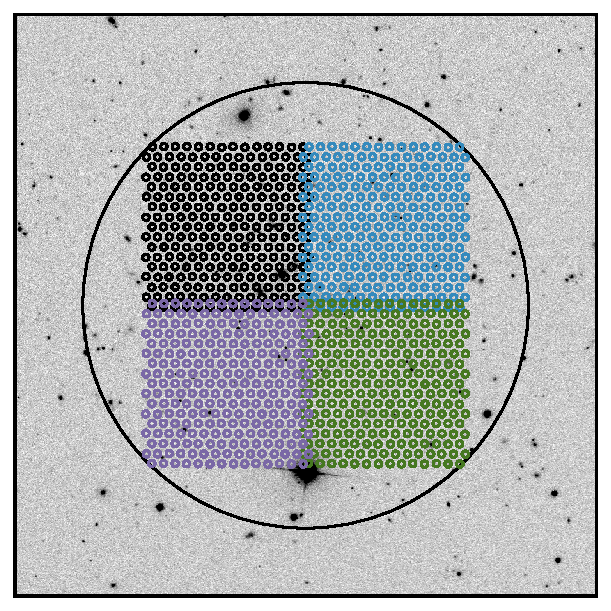
\includegraphics[width=0.6\textwidth]{./figures2/pointing.pdf} 
	\end{center}
	\caption[Basic properties of the ten galaxy clusters targeted with the MS.]{SDSS r-band image of an optically selected galaxy cluster Abell 2631 ($z=0.273$) selected from the SDSS DR8 data, and centered on the BCG. The large black circle shows the region $R<0.5$ Mpc ($r<2\farcm3$). The northeast (NE), northwest (NW), southwest (SW), and southeast (SE) fields with the fiber positions are shown in black, blue, green and purple respectively, illustrating how we survey each cluster. Nearly all galaxies within this region are associated with the cluster.}
	\label{2fig:tiles} 
\end{figure}

We use MS to target the galaxy clusters using the 5 \AAA\ grating covering a wavelength range of $4400 - 6600$ \AAA. With this instrumental setup and for galaxies $z = 0.2-0.3$, we will cover the Ca H\&K, Fe I ($\lambda 4383$), H-$\delta$, H-$\gamma$ and H-$\beta$ absorption features. Additionally, we cover emission of the \hbox{[\ion{O}{ii}]} ($\lambda\lambda 3727,3729$) doublet, H-$\beta$, and \hbox{[\ion{O}{iii}]} ($\lambda\lambda 4960,5008$), which allows for the identification of actively star-forming galaxies.

The FOV of the MS corresponds to an approximately 0.4 Mpc square region at $z = 0.2-0.3$. To ensure adequate coverage of the cluster out to a radius of 0.5 Mpc, we use four MS pointings per cluster. Figure~\ref{2fig:tiles} shows an example of the pointing pattern done on each cluster. The entire field is centered on the brightest cluster galaxy (BCG) and the individual tiles are shifted away. Furthermore, each of the four tiles are dithered at relative positions $(\Delta \alpha, \Delta \delta)=(0\farcs0,0\farcs0)$, $(-3\farcs6,-2\farcs0)$, and $(0\farcs0, -4\farcs0)$ from the origin to ensure full coverage of the FOV. Therefore, there are 736 individual spectra for each of the four fields or 2952 measurements for the cluster as a whole.

We have set exposure times to achieve spectra with signal-to-noise ratios (SNRs) $\sim3$ per spectral element (averaged over 4.6 pixels) in the continuum for objects with \sdssg\ $= 21.3$ mag (which corresponds to approximately 0.2L$^\star$ for cluster galaxies at $z = 0.2$) in 3600 seconds per pointing.. We base the expected SNR on the experience of \cite{Shetrone2010}, who achieves SNR $= 100$ per pixel in the continuum for point sources with B $=16.5$ mag at 4000 \AAA\ in 4800 seconds. We require 4 pointings to cover the full area for each cluster. Therefore, we require 1 hr/pointing $\times$ 4 pointings $= 4$ hrs on sky per cluster. Even though the field is dense with galaxies, there is sufficient ``blank'' area to allow for enough ``sky'' fibers for background subtraction.

\section{Data Reduction}\label{2sec:data reduction} 
All data are reduced using \textsc{p3d}\footnote{http://p3d.sourceforge.net/} \citep{Sandin2010} a general-use IFU reduction pipeline. The first step is to min/max-filtered average combine a minimum of 20 bias images from each night into a master-bias image, which is subtracted from each other image from the same night. Secondly, a trace mask is created from flat-fielding on the dusk or dawn sky. The fibers are fairly densely packed, so to determine the position of each spectrum in the dispersion direction each spectrum is extracted using a multi-profile deconvolution approach \citep{Sharp2010} to account for cross talk between fibers. Third, a dispersion mask for the wavelength calibration from images of Hg+Cd (for the May, 2012 observations) or Cd+Ne (for all other observations) arc lamps. The residuals between the derived wavelength solution and the known wavelengths of the emission lines is calculated from a fifth order polynomial and lie between $0.02 - 0.06$ \AAA. Finally, a fiber flat is created from the sky flats by a min/max-filtered average combine as in step one. 

We extracted the science spectra using several steps. First, we subtract the bias frames from each science frame. Next, we use \textsc{PyCosmic} \citep{Husemann2012}, integrated into \textsc{p3d} with the default parameters, to clean cosmic ray hits. Third, we use the previously created dispersion mask to wavelength calibrate the extracted spectra. Aligning the dispersion mask to bright telluric lines (namely \hbox{[\ion{O}{i}]} at 5577 \AAA) accounts for any flexure in the instrument between the images of the arc lamps and science frames. Finally, we normalize the extracted spectra using the transmission in the fiber flats from above. 

The result of this process is row-stacked spectra and associated pipeline-propagated uncertainties, where each of the 246 fibers are stored individually. A table of fiber positions maps each spectrum onto the image plane. However, for many of our observations a precise astrometric solution for the fiber positions is unknown. The position of the individual fibers can be recomputed by observing dense star fields after each telescope service in which the MS is involved. To correct our fiber positions we first identify fibers which observe stars and identify which fibers the astrometric solution indicates should contain stars. In many cases the stars are located between fibers. To account for this we use a simple Gaussian centroid weighted by the observed flux $5000 \leq \lambda \leq 5010$ \AAA\ to find the correct sky position of the star. We then shift the fiber grid to match the sky position of the stars as reported by the SDSS. Typical shifts are $0.5'' - 4''$, less than the width of a single fiber. For each observation we use as many stars as possible and combine the shifts to generate a mean offset. This offset is applied to all dithers of each observation. There is little need to obtain highly accurate fiber positions as the $4\farcs24$ fibers insures that reasonably correct positions will identify which fibers should and should not contain galaxies.

We use a simple sky subtraction scheme to remove the majority of sky contamination. Because the majority of fibers for any single pointing are empty, we use a $3\sigma$ clipped median selection to identify sky fibers and a simple mean to combine them. The result is then subtracted from every fiber. This adequately removes the bulk of sky emission lines, but often fails to completely remove the \hbox{[\ion{O}{i}]} line at 5577~\AAA. This line is masked throughout the determination of redshifts.

\begin{figure}[t]
\subfloat{%
  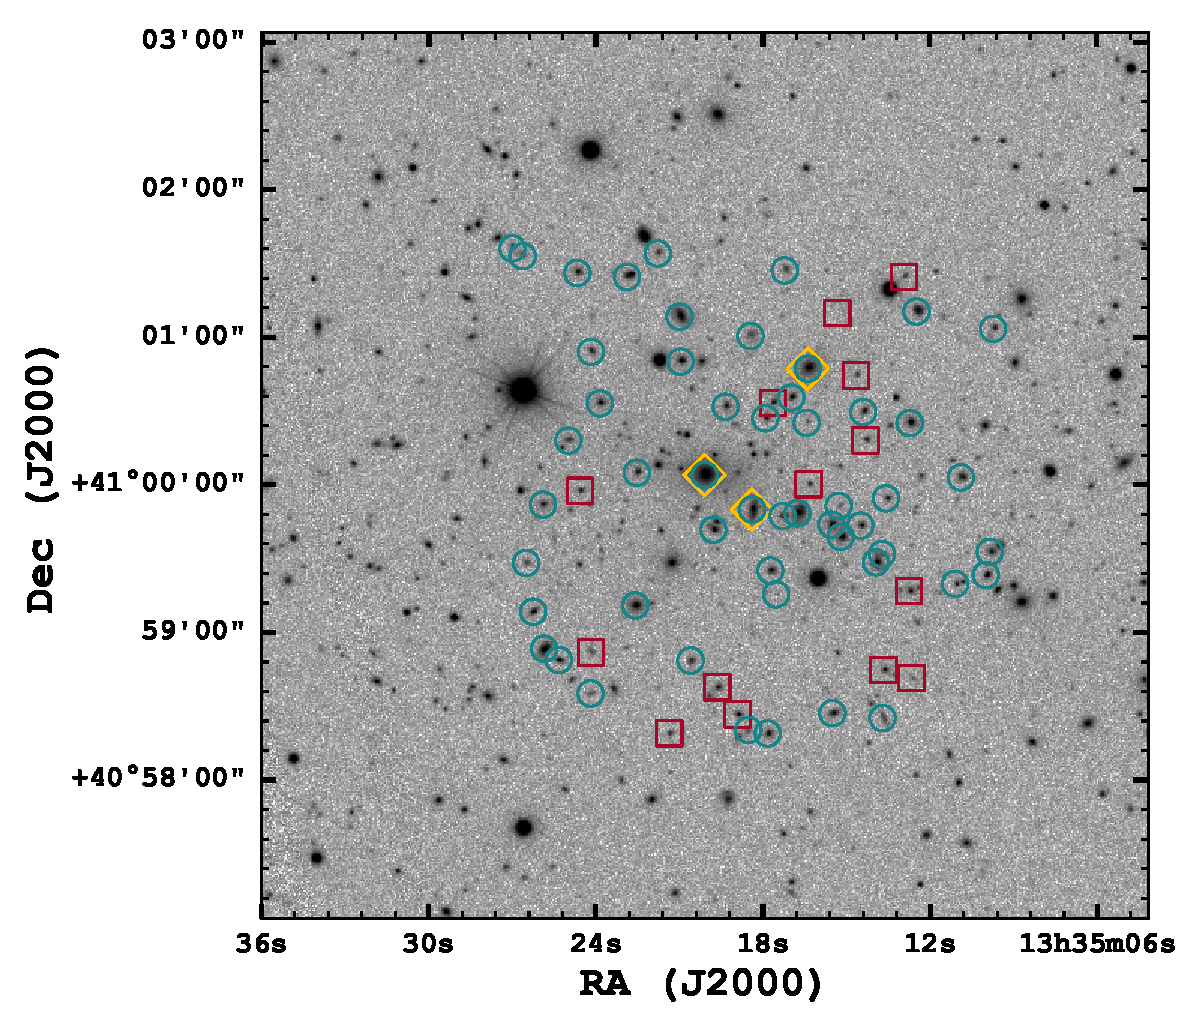
\includegraphics[width=0.5\textwidth]{./figures2/c203p83+41p0_mosaic.pdf}
}
\hfill
\subfloat{%
  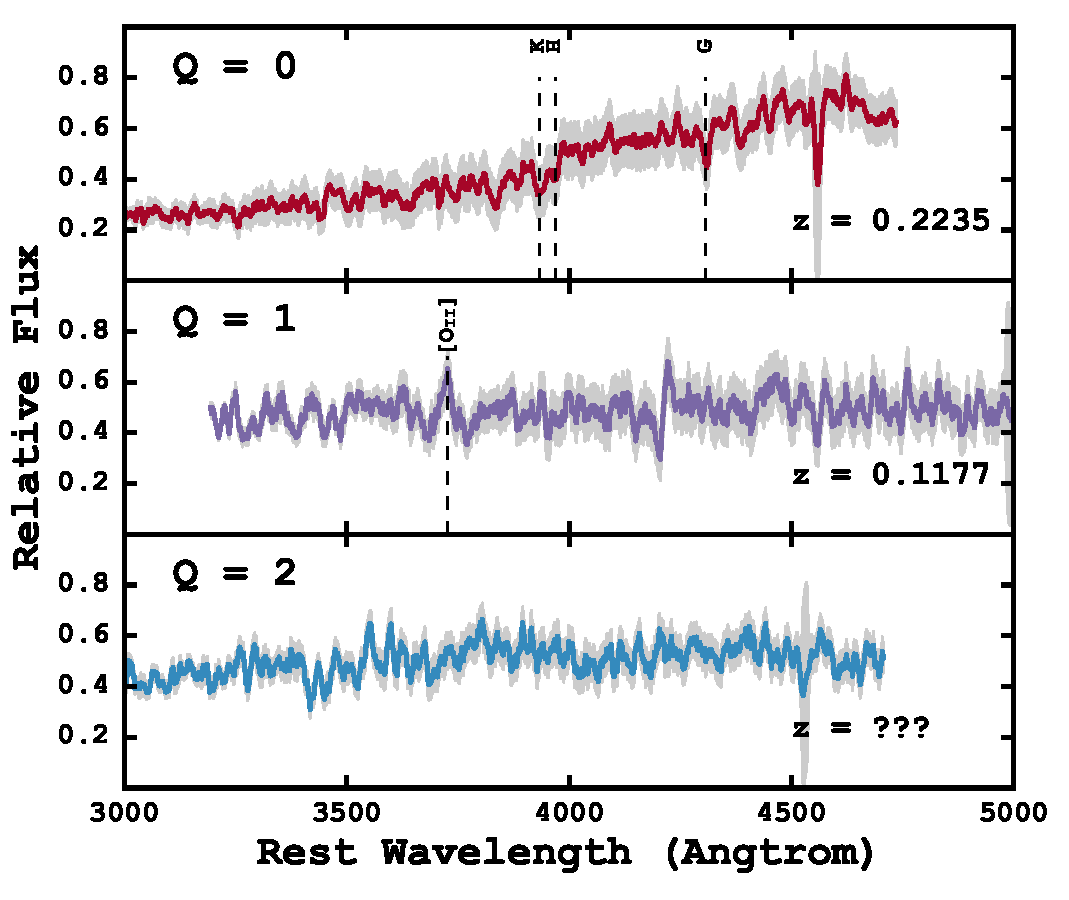
\includegraphics[width=0.5\textwidth]{./figures2/spectrum.pdf}
}
    \caption[SDSS \sdssr\ image of cluster VCSJ133520.1+410004.1 and spectra quality examples]{SDSS \sdssr\ image of cluster VCSJ133520.1+410004.1. The symbols show the position of observed galaxies. Turquoise circles indicate galaxies with $Q=0$ or $Q=1$ spectroscopic redshifts, red squares indicate galaxies where a redshift could not be reliably determined, and the yellow diamond corresponds to galaxies with pre-existing redshifts from the SDSS. \textit{Right:} Example spectra, with major features identified, showing the three quality flags. $Q=0$ represents the best quality spectra and $Q=2$ the poorest quality. Grey shaded regions show the {\sc p3d} internally estimated, relative errors. We take galaxies with $Q=0$ and $Q=1$ for the analysis in this study.} 
	\label{2fig:VCSJ133520.1+410004.1}
\end{figure}

After reducing all spectra we find an average residual mismatch in the wavelength solution of $\sigma_\lambda \sim 0.4$ \AAA\ or 24 \kms\ at 5000 \AAA. These residuals are small compared to the instrumental resolution. We find an average instrumental resolution of $\sim144$ \kms, and combining the two in quadrature gives a total instrumental resolution of $\sigma_{inst} = 146$ \kms, similar to that of other studies using the MS \citeeg{Murphy2011, Blanc2013}.

\section{Analysis}\label{2sec:analysis} 
The analysis of our reduced spectra occurs in two stages. First we derive individual redshifts using the observed galaxies, and then utilize the redshifts collectively to identify which galaxies likely belong to the galaxy cluster.

Individual galaxy selection is done through cross matching the IFU fiber sky positions with galaxies selected from the SDSS. To collect the galaxies from the SDSS, we select all galaxies with $\sdssg <$ 22 mag within $3'$ of the BCG in each cluster. For each cluster we create catalogs of photometry in all SDSS bands (\sdssu\sdssg\sdssr\sdssi\sdssz), photometric redshift, and any spectroscopic redshift.

Because of the large number of fiber pointings, only fibers which overlap with SDSS sources are considered for redshift analysis. The left panel of Figure \ref{2fig:VCSJ133520.1+410004.1} shows cluster VCSJ133520.1+410004.1 with the SDSS detections and measured redshifts overlaid. Orange diamonds are galaxies with SDSS available redshifts. The blue circles and red squares correspond to galaxies where a redshift was and was not determined from the observed spectra. See Figure~\ref{2fig:montage} for a similar representation of the remaining nine clusters.

\subsection{Redshift Catalog}\label{2sec:redshift catalog} 
A redshift solution is determined for each galaxy by cross-correlating \citep{Tonry1979} each of the spectra with six galaxy template spectra from the SDSS\footnote{http://classic.sdss.org/dr7/algorithms/spectemplates/index.html} using the \textsc{xcsao} task in the \textsc{iraf} \textsc{rvsao} package \citep{Kurtz1992, Kurtz1998}. For each galaxy we select the spectral template with the highest cross-correlation coefficient and visually inspect the fit. During visual inspection a quality flag ($Q$) is assigned. High-confidence redshifts, clearly determined by at least two obvious features (such as the Ca H, K and E absorption features), receive $Q=0$. Spectra with only a single strong feature (\eg, \hbox{[\ion{O}{ii}]} emission) are assigned $Q=1$. Redshifts resulting from enigmatic features are assigned $Q=2$. Figure~\ref{2fig:VCSJ133520.1+410004.1} shows representative example spectra for each of the $Q$ flags. For the determination of cluster properties we only consider galaxies with spectroscopic quality flags of $Q=0$ and $Q=1$. 

\begin{figure}[t]
	\begin{center}
		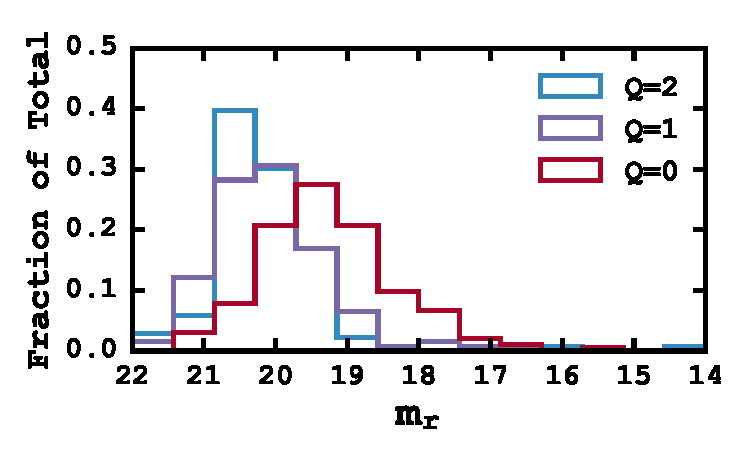
\includegraphics[width=0.6\textwidth]{figures2/redshiftHist.pdf}
	\end{center}
	\caption[Redshift recovery fractions across all clusters]{Redshift recovery fractions across all clusters. The bar heights represent the fraction of the total redshifts with the respective $Q$ value at a particular magnitude. For example, $\sim 40\%$ of the $Q=2$ redshifts have $m_r = 20.5-21$. We find a general decrease in redshift quality with increasing $m_r$. } 
	\label{2fig:redshiftHist} 
\end{figure}

Figure \ref{2fig:redshiftHist} shows the breakdown of $Q$ values for the redshifts across all clusters. We attempt to estimate spectroscopic redshifts for 447 galaxies, of which 44\% have $Q=0$, 27\% have $Q=1$ and 29\% have $Q=2$.  We find a general decrease in $Q$ flag with increasing $m_r$. Approximately 30\% of the $Q=0$ redshifts correspond to galaxies with $19 < m_r <20$ mag whereas about 40\% $Q=2$ galaxies have $m_r = 20.5-21$ mag.

\begin{landscape}
	\singlespace
	\begin{longtable}{ccccccccccc} 
	\caption[Spectroscopic redshifts for galaxies in VCSJ133520.1+410004.1]{Spectroscopic redshifts for galaxies in VCSJ133520.1+410004.1 measured with the MS: Column 1: The telescope pointing; Column 2: The dither position; Column 3: The fiber number; Column 4: The right ascension of the galaxy; Column 5: The declination of the galaxy; Column 6: The the observed SDSS \sdssr\ magnitude; Column 7: The galaxy redshift; Column 8: The redshift $Q$ flag; Column 9: The galaxy membership information; Column 10: The clustercentric radial distance; Column 11: The LOSV of the galaxy with respect to the cluster. See the appendix for similar tables for the remaining nine clusters.}\\
	\hline
	tile & dither & fiber & RA (J2000) & DEC (J2000) & \sdssr\ (mag) & redshift & $Q$ & Member & R (Mpc) & LOSV (\kms) \\
	(1) & (2) & (3) & (4) & (5) & (6) & (7) & (8) & (9) & (10) & (11) \\
	\hline \hline
	\endfirsthead
	\multicolumn{4}{l}%
	{\tablename\ \thetable\ Continued} \\
	\hline
	tile & dither & fiber & RA (J2000) & DEC (J2000) & \sdssr\ (mag) & redshift & $Q$ & Member & R (Mpc) & LOSV (\kms) \\
	(1) & (2) & (3) & (4) & (5) & (6) & (7) & (8) & (9) & (10) & (11) \\
	\hline \hline
	\endhead
		NE & 1 & 14 & 13:35:27.004 & +41:01:36.20 & 20.47 & 0.2019$\pm{0.0003}$ & 1 & ... & 0.40 & -6945$\pm{146}$ \\
		NE & 1 & 111 & 13:35:24.177 & +41:00:54.16 & 20.10 & 0.1178$\pm{0.0001}$ & 1 & ... & 0.15 & -27397$\pm{63}$ \\
		NE & 1 & 154 & 13:35:23.853 & +41:00:33.19 & 19.28 & 0.2214$\pm{0.0002}$ & 0 & ... & 0.18 & -2214$\pm{83}$ \\
		NE & 2 & 6 & 13:35:21.777 & +41:01:34.15 & 20.38 & 0.1691$\pm{0.0002}$ & 1 & ... & 0.27 & -14929$\pm{102}$ \\
		NE & 2 & 14 & 13:35:26.632 & +41:01:33.06 & 20.95 & 0.0403$\pm{0.0003}$ & 0 & ... & 0.09 & -46214$\pm{131}$ \\
		NE & 2 & 63 & 13:35:20.998 & +41:01:08.49 & 17.90 & 0.2381$\pm{0.0001}$ & 0 & $\checkmark$ & 0.25 & 1849$\pm{49}$ \\
		NE & 3 & 22 & 13:35:22.879 & +41:01:24.60 & 19.76 & 0.2386$\pm{0.0003}$ & 0 & $\checkmark$ & 0.33 & 1961$\pm{131}$ \\
		NE & 3 & 25 & 13:35:24.669 & +41:01:26.21 & 19.54 & 0.1444$\pm{0.0001}$ & 0 & ... & 0.25 & -20924$\pm{58}$ \\
		NE & 3 & 73 & 13:35:18.447 & +41:01:00.60 & 19.63 & 0.0779$\pm{0.0001}$ & 0 & ... & 0.09 & -37080$\pm{29}$ \\
		NE & 3 & 106 & 13:35:20.957 & +41:00:50.19 & 18.83 & 0.2235$\pm{0.0002}$ & 0 & $\checkmark$ & 0.17 & -1691$\pm{78}$ \\
		NE & 3 & 147 & 13:35:19.341 & +41:00:31.82 & 19.48 & 0.2380$\pm{0.0001}$ & 0 & ... & 0.11 & 1822$\pm{73}$ \\
		NE & 3 & 185 & 13:35:24.990 & +41:00:18.06 & 20.51 & 0.1887$\pm{0.0002}$ & 1 & ... & 0.18 & -10169$\pm{83}$ \\
		NE & 3 & 206 & 13:35:20.095 & +41:00:04.12 & 16.39 & 0.2274$\pm{0.0001}$ & 1 & $\checkmark$ & 0.00 & -763$\pm{34}$ \\
		NE & 3 & 210 & 13:35:22.528 & +41:00:05.00 & 19.59 & 0.2242$\pm{0.0001}$ & 1 & $\checkmark$ & 0.10 & -1543$\pm{49}$ \\
		NW & 1 & 127 & 13:35:16.384 & +41:00:47.33 & 17.43 & 0.2377$\pm{0.0001}$ & 0 & $\checkmark$ & 0.23 & 1752$\pm{68}$ \\
		NW & 1 & 167 & 13:35:14.400 & +41:00:29.73 & 19.69 & 0.2333$\pm{0.0002}$ & 0 & $\checkmark$ & 0.26 & 690$\pm{117}$ \\
		NW & 2 & 27 & 13:35:17.216 & +41:01:27.25 & 20.21 & 0.1512$\pm{0.0002}$ & 0 & ... & 0.24 & -19279$\pm{117}$ \\
		NW & 2 & 63 & 13:35:12.486 & +41:01:10.57 & 18.84 & 0.1638$\pm{0.0001}$ & 0 & ... & 0.31 & -16210$\pm{44}$ \\
		NW & 2 & 73 & 13:35:09.729 & +41:01:03.49 & 20.00 & 0.2402$\pm{0.0001}$ & 1 & ... & 0.50 & 2367$\pm{58}$ \\
		NW & 2 & 165 & 13:35:12.728 & +41:00:25.16 & 18.74 & 0.2394$\pm{0.0001}$ & 0 & $\checkmark$ & 0.33 & 2155$\pm{58}$ \\
		NW & 2 & 171 & 13:35:16.434 & +41:00:25.31 & 21.68 & 0.1617$\pm{0.0002}$ & 1 & ... & 0.13 & -16728$\pm{121}$ \\
		NW & 2 & 173 & 13:35:17.911 & +41:00:27.16 & 19.49 & 0.1039$\pm{0.0002}$ & 0 & ... & 0.06 & -30763$\pm{107}$ \\
		NW & 2 & 220 & 13:35:10.891 & +41:00:03.07 & 19.45 & 0.2994$\pm{0.0002}$ & 0 & ... & 0.47 & 16739$\pm{102}$ \\
		NW & 2 & 239 & 13:35:13.582 & +40:59:54.58 & 20.24 & 0.2316$\pm{0.0002}$ & 1 & $\checkmark$ & 0.28 & 265$\pm{92}$ \\
		NW & 3 & 142 & 13:35:16.981 & +41:00:35.55 & 19.44 & 0.2233$\pm{0.0002}$ & 0 & $\checkmark$ & 0.17 & -1745$\pm{78}$ \\
		SE & 1 & 27 & 13:35:25.896 & +40:59:52.05 & 19.35 & 0.2295$\pm{0.0004}$ & 1 & $\checkmark$ & 0.25 & -238$\pm{170}$ \\
		SE & 1 & 46 & 13:35:19.779 & +40:59:41.85 & 18.73 & 0.2293$\pm{0.0002}$ & 0 & $\checkmark$ & 0.08 & -284$\pm{107}$ \\
		SE & 1 & 86 & 13:35:26.506 & +40:59:28.30 & 20.59 & 0.2255$\pm{0.0002}$ & 1 & $\checkmark$ & 0.29 & -1205$\pm{112}$ \\
		SE & 1 & 123 & 13:35:22.588 & +40:59:11.02 & 18.17 & 0.2307$\pm{0.0002}$ & 0 & $\checkmark$ & 0.22 & 44$\pm{102}$ \\
		SE & 1 & 129 & 13:35:26.254 & +40:59:08.50 & 19.42 & 0.1282$\pm{0.0002}$ & 0 & ... & 0.20 & -24863$\pm{107}$ \\
		SE & 2 & 164 & 13:35:20.600 & +40:58:48.65 & 20.02 & 0.2938$\pm{0.0001}$ & 0 & ... & 0.33 & 15369$\pm{53}$ \\
		SE & 3 & 157 & 13:35:25.857 & +40:58:53.46 & 18.31 & 0.1701$\pm{0.0001}$ & 0 & ... & 0.28 & -14684$\pm{29}$ \\
		SE & 3 & 171 & 13:35:25.332 & +40:58:48.88 & 19.49 & 0.2400$\pm{0.0003}$ & 0 & ... & 0.36 & 2296$\pm{126}$ \\
		SE & 3 & 198 & 13:35:24.191 & +40:58:35.23 & 20.83 & 0.1177$\pm{0.0002}$ & 1 & ... & 0.21 & -27419$\pm{87}$ \\
		SW & 1 & 41 & 13:35:17.295 & +40:59:47.40 & 19.87 & 0.2231$\pm{0.0002}$ & 0 & ... & 0.13 & -1808$\pm{107}$ \\
		SW & 1 & 114 & 13:35:17.529 & +40:59:15.55 & 20.60 & 0.2493$\pm{0.0003}$ & 1 & ... & 0.22 & 4561$\pm{156}$ \\
		SW & 1 & 224 & 13:35:13.709 & +40:58:25.25 & 20.03 & 0.1276$\pm{0.0003}$ & 0 & ... & 0.28 & -25006$\pm{126}$ \\
		SW & 1 & 227 & 13:35:15.509 & +40:58:27.26 & 19.27 & 0.2328$\pm{0.0002}$ & 0 & $\checkmark$ & 0.41 & 559$\pm{83}$ \\
		SW & 1 & 245 & 13:35:17.832 & +40:58:19.02 & 19.29 & 0.2211$\pm{0.0003}$ & 1 & ... & 0.39 & -2275$\pm{136}$ \\
		SW & 1 & 246 & 13:35:18.529 & +40:58:20.43 & 21.31 & 0.1970$\pm{0.0002}$ & 1 & ... & 0.34 & -8140$\pm{117}$ \\
		SW & 2 & 24 & 13:35:15.282 & +40:59:51.52 & 21.29 & 0.2225$\pm{0.0002}$ & 1 & $\checkmark$ & 0.20 & -1934$\pm{97}$ \\
		SW & 2 & 29 & 13:35:18.391 & +40:59:50.06 & 18.17 & 0.2405$\pm{0.0001}$ & 0 & ... & 0.09 & 2440$\pm{44}$ \\
		SW & 2 & 39 & 13:35:15.539 & +40:59:43.86 & 18.73 & 0.2263$\pm{0.0002}$ & 0 & $\checkmark$ & 0.20 & -1023$\pm{107}$ \\
		SW & 2 & 53 & 13:35:15.211 & +40:59:38.90 & 18.73 & 0.2412$\pm{0.0001}$ & 0 & $\checkmark$ & 0.23 & 2593$\pm{58}$ \\
		SW & 2 & 59 & 13:35:09.857 & +40:59:32.82 & 19.83 & 0.2334$\pm{0.0002}$ & 1 & $\checkmark$ & 0.45 & 697$\pm{107}$ \\
		SW & 2 & 65 & 13:35:13.725 & +40:59:31.94 & 20.58 & 0.3156$\pm{0.0003}$ & 0 & ... & 0.37 & 20688$\pm{156}$ \\
		SW & 2 & 86 & 13:35:17.737 & +40:59:25.25 & 19.71 & 0.2236$\pm{0.0002}$ & 0 & $\checkmark$ & 0.17 & -1684$\pm{78}$ \\
		SW & 2 & 90 & 13:35:11.098 & +40:59:19.79 & 20.41 & 0.2354$\pm{0.0002}$ & 0 & $\checkmark$ & 0.42 & 1195$\pm{97}$ \\
		SW & 3 & 26 & 13:35:16.763 & +40:59:48.52 & 17.94 & 0.2250$\pm{0.0001}$ & 0 & $\checkmark$ & 0.15 & -1334$\pm{34}$ \\
		SW & 3 & 37 & 13:35:14.503 & +40:59:43.50 & 19.79 & 0.2428$\pm{0.0002}$ & 0 & $\checkmark$ & 0.26 & 2979$\pm{107}$ \\
		SW & 3 & 65 & 13:35:13.944 & +40:59:28.57 & 18.60 & 0.2362$\pm{0.0001}$ & 0 & $\checkmark$ & 0.29 & 1385$\pm{58}$ \\
		SW & 3 & 73 & 13:35:10.002 & +40:59:23.42 & 19.52 & 0.2307$\pm{0.0001}$ & 0 & $\checkmark$ & 0.45 & 39$\pm{73}$ \\
	\hline 
	\label{2tbl:VCSJ133520.1+410004.1} 
	\end{longtable}
\end{landscape}

\textsc{xcsao} reports errors on the cross-correlation redshift. Previous work \citeeg{Quintana2000, Sifon2015a} show the cross-correlation velocity uncertainties by up to a factor of two. We report our redshift uncertainties as twice the uncertainty estimated by \textsc{xcsao}.

Redshift information, with $Q=0$ or $Q=1$ spectra, for each galaxy are given in Table~\ref{2tbl:VCSJ133520.1+410004.1}. The right panel of Figure~\ref{2fig:VCSJ133520.1+410004.1} shows selected spectra from cluster VCSJ133520.1+410004.1 with corresponding best fitting SDSS template. See the appendix for similar examples from the remaining nine clusters.

\subsection{Cluster Membership}\label{2sec:cluster membership} 
We first determine the cluster central redshift. This serves as a zero-point from which all other galaxies will be compared. Therefore, the accurate determination of the cluster redshift ($z_c$) is crucial to the reliability of all following measurements. An incorrect cluster redshift introduces errors into the measured line of sight velocity (LOSV) and corresponding dispersion, which, in turn, contributes to errors associated with dynamical mass and radius. 

In simple terms, the cluster redshift is the mean of the redshifts of all galaxies associated with the cluster. However, because the standard mean can be quite sensitive to outliers or otherwise contaminated data, we require a more resistant statistic, and turn to the biweight location estimator \citep{Beers1990} which provides improved performance. The biweight location does not give us the freedom to use all galaxies measured but provides protection against a small number of interlopers. Therefore, the process of determining $z_c$ and the cluster membership are linked. We begin with the nominal $z_c$ (see Table~\ref{2tbl:targets}) and apply and initial velocity cut of 5000 \kms\ to remove any foreground or background galaxies. Then, using the membership determination techniques described below we determine the member galaxies from which a new $z_c$ is calculated. The entire process is repeated until convergence, usually within a single iteration. The cluster central redshift and associated 68\% uncertainties, derived from bootstrap resampling, are given in Table~\ref{2tbl: derived parameters}.

To reject the galaxies not associated with the targeted cluster, we employ two methods depending on the number of galaxies associated with each cluster. For clusters with 20 or more $Q=0$ or $Q=1$ redshifts we use the ``shifting gapper'' method of \citeeg{Fadda1996, Crawford2014}, which combines both the positional and velocity information. Galaxies are first sorted by their radial separation from the cluster center (See Table~\ref{2tbl:targets}) and binned into radial bins of at least 10 members. Once in the radial bins, the galaxies are sorted by the LOSV, 
\begin{equation}
	LOSV = c\frac{(z-z_{c})}{(1+z_{c})} 
\end{equation}
where $c$ is the speed of light in \kms, $z$ is the redshift of the individual galaxy and $z_{c}$ is the redshift of the cluster. Any galaxy with a LOSV greater than 1000 \kms of a neighboring galaxy (the velocity ``gap'') is rejected as an interloper. The procedure repeats until the number of galaxies stabilizes in the bin. Once the members have been identified we recompute $z_c$, LOSVs, and begin the membership selection again. This entire process is repeated until the number of member galaxies remains constant. This is normally achieved within a single iteration. 

For galaxy clusters with fewer than 20 $Q=0$ or $Q=1$ redshifts we employ the general of membership determination method outlined in \cite{Wilman2005, Connelly2012}. We assume an initial velocity dispersion, $\sigma(v)$, of 500$(1+z)$ \kms\ and apply both redshift and spatial limits given by: 
\begin{equation}
	\delta(z)_{max} = 2 \sigma(v)/c 
\end{equation}
and 
\begin{equation}
	\delta(r)_{max} = \frac{c\times\delta(z)_{max}}{bH(z)} 
\end{equation}
where $b=9.5$ is the aspect ratio between the projected spatial and line-of-sight dimensions, $H(z) = H_0 E(z)$ and $E(z) = \sqrt{\Omega_m(1+z^3)+\Omega_{\Lambda}}$. We select all galaxies with $|z-z_c| < \delta(z)_{max}$ and radial separation, $R$, $<\delta(r)_{max}$. During each step, we update both the $z_c$ and $\sigma(v)$ using the identified members and this process is repeated until the number of member galaxies converges, usually within three iterations.

To calculate the velocity dispersion in this membership determination method, we use the gapper estimator \citep{Beers1990} which provides accurate dispersions for groups as small as five members \citep{Hou2009}. It is given by 
\begin{equation}
	\sigma_g = \frac{\sqrt{\pi}}{N(N-1)} \sum_{i=1}^{N-1} w_i g_i
\end{equation}
where $N$ is the number galaxies, the weights are $w_i = i(N-i)$ and $g_i = LOSV_{i+1} - LOSV_i$ are the gaps between ordered pairs of radial LOSVs. The aspect  The dispersion estimate is corrected by $1.135$ to account for the $2\sigma$ redshift space cut applied during membership determination \citep{Connelly2012}. We follow this method for the calculation of the dispersion for consistency in member determination only. The final velocity dispersion of each cluster is determined in the following subsection.

Membership information for the galaxies observed in and around cluster VCSJ133520.1+410004.1 is given in Column 9 of Table~\ref{2tbl:VCSJ133520.1+410004.1}. See the appendix for the membership of the other observed clusters.

\subsection{Line-of-Sight Velocity Dispersion}\label{2sec:LOSVD}
To compute the line-of-sight velocity dispersion (LOSVD) of each cluster we follow the maximum likelihood method of \cite{Walker2006}. We assume that the each galaxy is drawn from a Gaussian distribution centered on the mean cluster velocity and we maximize the log of the product of each cluster member's individual Gaussian probabilities (their Eq. 8):
\begin{equation}
  \label{2eq:log}
\ln(p)=-\frac{1}{2}\sum_{i=1}^{N}\ln(\sigma_i^2+\sigma_p^2)-\frac{1}{2}\sum_{i=1}^N\frac{(v_i-\langle u \rangle)^2}{(\sigma_i^2+\sigma_p^2)}-\frac{N}{2}\ln(2\pi).
\end{equation}
where $N$ is the number of member galaxies, $\sigma_p$, $\langle\mu\rangle$, and $\sigma_i$ is the LOSVD, the average radial velocity and the error on the individual LOSVs respectively. To maximize the probability, we use {\sc emcee}\footnote{http://dan.iel.fm/emcee/current/} \citep{Foreman-Mackey2013}, a Monte Carlo Markov Chain (MCMC) sampler, based on affine-invariant ensemble sampler (see \citealt{Goodman2010} for details on affine-invariant samplers). We set priors on $\langle\mu\rangle$, and $\sigma_p$ by requiring that $\langle\mu\rangle$ lies between the maximum and minimum LOSV and that $\sigma_p$ be positive and less than $1400$ \kms which corresponds approximately to a $10^{16}$ \Msol\ cluster at $z=0$, larger than any expected cluster mass in our sample. We draw twenty thousand samples from the posterior probability distribution and report a measured LOSVD as the median value of the posterior probability distribution with 68\% error bars defined as the square root of the second moment of the same distribution.

\section{Estimating Cluster Masses}
The goal of this section is to describe the methods used to estimate (or predict) the total masses of the clusters in our sample. We test two distinct approaches. We begin the discussion with a traditional power law (PL) based approach where we estimate the cluster mass based on the LOSVD measurement. The second is a machine learning (ML) based approach where we use a combination of cluster observables to predict a cluster mass. The ML approach requires additional discussion about the creation of a suitable training set. We conclude with an examination of how this training set can potentially influence the results of the ML method.   

\subsection{PL Estimates of Cluster Mass}
We adopt the scaling relation of \cite{Munari2013} to estimate cluster masses based solely on their LOSVD. The scaling relation is based on the work of \cite{Evrard2008} and has the form: 
\begin{equation}\label{2eq:power law}
	M_{200c} = \frac{10^{15}}{h(z)} \bigg{(}\frac{\sigma_{1D}}{A_{1D}} \bigg{)}^{1/\alpha} \Msol 
\end{equation}
where $A_{1D} =1177\pm4.2$ \kms, $\alpha = 0.364\pm0.0021$, $h(z) = H(z)/100$, and $\sigma_{1D}$ is the LOSVD. The relation is calibrated through a cosmological simulation using galaxies (instead of dark matter particles or subhalos) as the tracers of LOSVD. This choice of tracer results in dynamical masses which are $16-26\%$ lower \citeeg{Kirk2015, Sifon2015a} than masses obtained through the scaling relation of \cite{Evrard2008}, which has been calibrated using dark matter particles alone. This is due dynamical effects which act upon the galaxies but not the dark matter particles.

We use the cluster redshift, given in Column 5, and the LOSVD values given in Column 6 of Table~\ref{2tbl: derived parameters} along with Equation~\ref{2eq:power law} to estimate the total mass of our ten clusters. The log of the estimated mass for each cluster is given in Column 7 of Table~\ref{2tbl: derived parameters}.

\subsection{Supervised Machine Learning}\label{2sec:ML methods}
Supervised ML provides an algorithm to infer the relationship between a set of known input variables (features) and a set of desired outputs (targets), through the use of a training set. The training set consists of both features and desired targets, which the ML algorithm uses to ``learn'' their relationship. The algorithm is then provided with a set of features alone, and uses the inferred relationship to predict appropriate target values. Part of the training set is often reserved as a \emph{testing} set \citeeg{Ripley2007, Xu2013, Ntampaka2015, Ntampaka2015a, Acquaviva2016} which is used to both select and train the specific ML algorithm.

Just as in \citetalias{Boada2016}, we rely on an ensemble ML method \citeeg{Caruana2006} known as a forest of randomized decision trees (or random forest; RF; \citealt{Ho1995, Ho1998}), which we prefer due to their straightforward design and easily accessible uncertainty estimates. A RF is a type of ensemble method where the trees can be visualized as flow chart. The path through the flow chart (the trees) is decided by the values of the training features at each fork. RF use a random subset of the train data to decide which fork should be followed. The final prediction is the mean of each tree's final value. We optimize the input parameters (often called hyper-parameters) of our RF by further splitting our testing set into a cross-validation (CV) set. We use 5-fold CV, where the testing set is split (folded) five times, throughout. The RF methods implemented in this work are part of the {\sc Scikit-Learn} \citep{Pedregosa2012} Python library.

Building off the work in \citetalias{Boada2016}, we use the ``Buzzard'' semi-analytical model to provide both the observable features and desired targets in order to train our ML method. The Buzzard mock galaxy catalog contains 238 million galaxies with \sdssr\ mag $< 29$ and $z \leq 8.7$. The galaxies are located in a 398.49 \degsq\ portion of the sky and their luminosities are derived from a combination of Sub-halo Abundance Matching (SHAM; \citealt{Reddick2013}) and Adding Density Dependent Spectral Energy Distributions (ADDSED). The galaxies are assigned to the dark matter halos identified by the {\sc ROCKSTAR} halo finder \citep{Behroozi2013}. The catalogs assume the following cosmological parameters: $\Omega_\Lambda = 0.714$, $\Omega_M = 0.286$, $\sigma_8 = 0.82$ and $H_0= 70$ \kms \mpc, which we have also adopted for general use in this work. See \citetalias{Boada2016} for a more thorough description of the process used to create the catalogs.

\subsection{ML Based Observations}

In order to create a mock dataset which resembles our actual observations we first rely on the RF method as a classifier. The goal is to assign each galaxy in the Buzzard catalog a $Q$ flag of either 0, 1 or 2 based on their observed magitudes in the five SDSS filters, \sdssu\sdssg\sdssr\sdssi\sdssz, the ten combinations of possible colors, and the square of those colors. \cite{Acquaviva2016} uses a similar feature set to predict the metallicity of SDSS galaxies with good effect. 

The classifier is trained using the redshift catalog derived from our cluster observations (Section \ref{2sec:redshift catalog}), and the 447 observations are split into a training, CV and test sample. We use the training set to train the ML method, the CV set to tune the model hyper-parameters and the test sample to verify how well our model classifies each galaxy. We also perform recursive feature elimination to remove features which contribute very little to the classification.

We compute two statistics to evaluate how well our model classifies the galaxies, the recall and the precision. The recall is the number predicted compared to the true number of classifications, $N_{pred}/N_{true}$. The precision is the number of correct predictions compared to the total number of predictions for each class, $N_{corr}/N_{pred}$. In both cases the metrics range from zero to one, and higher numbers are better. For our optimized RF classifier we achieve overall recall and precision of $\sim60\%$. For the individual classes ($Q$ flags), the RF classifier performs significantly better when classifying $Q=0$ and $Q=2$ galaxies, with recall rates well above 70\%. The $Q=1$ training galaxies have significant overlap between $Q=0$ and $Q=2$ (see Figure \ref{2fig:redshiftHist}) which leads to a recall for $Q=1$ galaxies of only $\sim20\%$. 

This is a difficult problem. Figure~\ref{2fig:redshiftHist} shows there is significant overlap between the $Q$ flags. In our testing, we find no combination of features which wholly separates the $Q$ flags, providing a high level of confusion for the RF. We find similar levels of recall and precision for other ML classification methods besides RF.

\begin{figure}[t]
	\begin{center}
		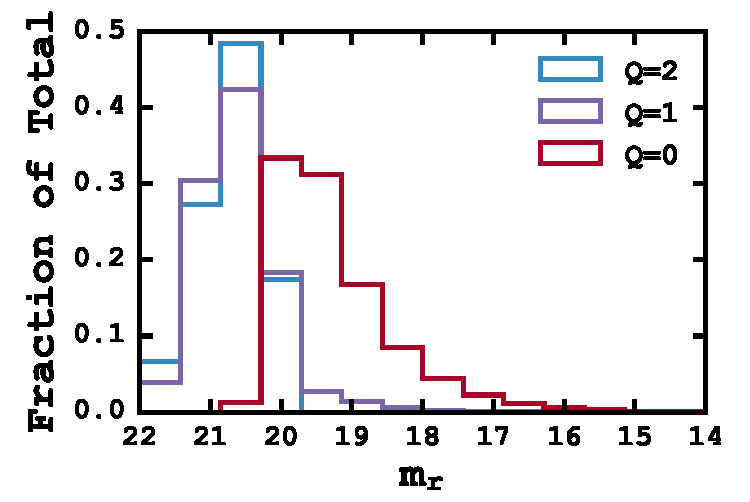
\includegraphics[width=0.6\textwidth]{figures2/buzzardQHist.pdf}
	\end{center}
	\caption[Quality flag assignments for the 2.7 million Buzzard catalog galaxies]{Quality flag ($Q$) assignments for the 2.7 million Buzzard catalog galaxies with $\sdssg< 22$ mag. The bar heights represent the fraction of the total redshifts with the respective $Q$ value at a particular magnitude. The distributions resemble the actual observations in Figure \ref{2fig:redshiftHist}. See the text for a detailed explanation of the classification process.} 
	\label{2fig:buzzardHist} 
\end{figure}

We assign each galaxy in the Buzzard catalog with $z<0.5$ and $\sdssg< 22$ mag a $Q$ flag using the optimized RF classifier trained with all 447 observations. Figure \ref{2fig:buzzardHist} shows the $Q$ flag distribution as a function of \sdssr\ magnitude. The total distribution of the 2.7 million $Q$ flags is 45.6\% $Q=0$, 24.7\% $Q=1$, and 29.6\% $Q=2$. This distribution closely resembles the fractions of the actual observations with some $Q=1$ galaxies misclassified as $Q=0$. Because we use galaxies with either $Q=0$ or $Q=1$ this is does not significantly bias our analysis.

\subsection{ML Based Cluster Masses}\label{2sec:ML based cluster masses}
We use the ``observed'' ($Q=0$ and $Q=1$) galaxies created in the previous subsection to construct total mass distributions of the mock clusters. For this task we again use a RF, not as a classifier but as a regressor, which predicts a cluster mass given a set of input features, such as the observed LOSVD and redshift. Similarly to our classification methods, we create an optimized ML method by splitting the Buzzard catalogs into a training, CV, and testing set. 

Because the cluster masses presented with this method are predictions based on the feature data, any uncertainties quoted by this method are prediction intervals not confidence intervals. Prediction intervals are an estimate of the interval encompassing future observations, with a given probability. Confidence intervals, on the other hand, describe the different moments of a population. The prediction intervals are unique to each prediction, and are often based on the underlying assumption of normally distributed residuals. RF estimators do not assume normally distributed residuals, and thus, require special treatment.  

The prediction intervals for our RF estimator as based on the method of quantile regression forests \citep{Meinshausen2006}. The basic principle is that we record all response variables (the predictions), not simply the mean. This allows us to give the prediction as the full conditional probability distribution of all possible predictions. For brevity, we quote predicted masses as the median prediction and the 68\% prediction interval as the square root of the second moment of the full conditional probability distribution.

\subsection{The Importance of Training Features}\label{2sec: training features}
\begin{figure}[t]
	\begin{center}
		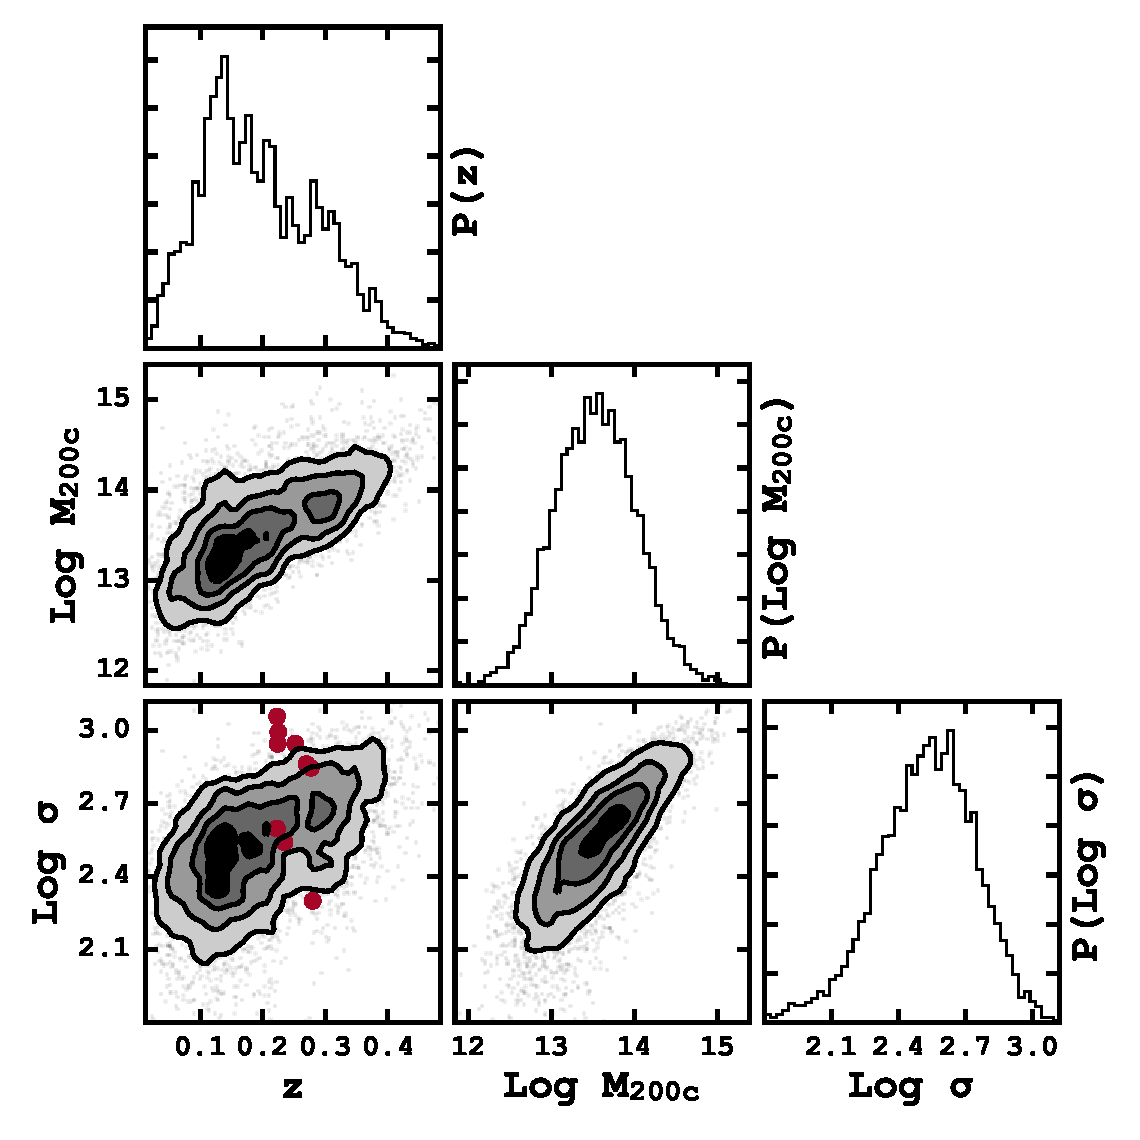
\includegraphics[width=0.6\textwidth]{figures2/buzzardCorner.pdf}
	\end{center}
	\caption[Corner plot of the \emph{training} data with features $\sigma$ and $z$.]{Contour plot of the \emph{training} data with features $\sigma$ and $z$. The corner plots shows all of the one and two dimensional posterior probability distributions used to determine the correct cluster mass. The colored circles show the position in the log $\sigma$-redshift plane of the ten clusters in this sample.}
	\label{2fig:buzzardCorner}
\end{figure}

The data used to train our ML algorithm is critical to the success of the method. We require training data which is broad enough to expose the ML method to a wide enough range of cluster parameters as not to influence the final outcome. The features of our training sample can be selected such that it does not bias the final predictions in an expected way. Figure~\ref{2fig:buzzardCorner} shows the $\sigma$ and $z$ features of the training sample from the Buzzard catalogs.\footnote{Contour plots based on \cite{Foreman-Mackey2016}.} The large red circles indicate the observed positions of our ten clusters in relation to the training data. Immediately noticeable, is that our observed clusters occupy a narrow redshift range ($0.2< z <0.3$). We also notice that seven of the ten clusters sit at the top edge of the training data in the $z$-log $\sigma$ plane. Because the observed clusters are separate from the training data, the accuracy of the predictions of the cluster masses will be diminished. 

Because the of the difference in cosmological volume covered by the SDSS and simulated by Buzzard, there are too few clusters in Buzzard, at $z\sim2$, and with $\sigma$ as large as the clusters in our sample. Predictions based on the Buzzard catalogs give a higher likelihood that clusters at $z\sim2$ will be of lower total mass, when the redshift is included as a feature. This becomes apparent by examining the $z$-log $M_{200c}$ plane in Figure~\ref{2fig:buzzardCorner}. The vast majority of clusters with $0.2< z <0.3$ have masses between $10^{13} - 10^{14}$ \Msol, whereas the observed LOSVD ($\sigma$) values of our clusters would place them above $10^{15}$ \Msol. 

To combat the effect of cluster mass under-prediction, we make two critical changes from our method presented in \citetalias{Boada2016}. First, instead of using the membership information provided by the Buzzard catalogs we observe the clusters much in the same way we have with our actual observations. We select all galaxies within $2\farcm3$ around the center of each cluster (see Figure~\ref{2fig:tiles} for an illustration), and determine the cluster membership using the methods described in Section~\ref{2sec:cluster membership}. This serves to broaden the LOSVD distribution of the training data as both true member galaxies will be excluded and interloping galaxies will be erroneously included. Secondly, we exclude the redshift information from the training features when predicting the cluster masses. This has the effect of flattening the HMF, allowing for high mass clusters to exist at all redshifts. However, the fewer training features also lowers the predictive power through an increase in both the bias and scatter (see Figure 6 in \citetalias{Boada2016} as an example). 

\section{Results and Discussion}\label{2sec:results}
The goal of this work to perform a practical test of some of the potential applications of a HETDEX-like survey to cluster science. Here, we present the predicted total masses of our ten clusters and estimate the absolute scale and scatter of a richness-mass relation based on those cluster masses. Because the accuracy of the predicted cluster masses is paramount to a well constrained richness-mass relation, we combine our results presentation with a discussion on their accuracy. 
 
\subsection{Cluster Masses}
\begin{figure} 
	% \includegraphics[width=\columnwidth]{figures/MLcomparison_shifty.pdf}
	\begin{center}
		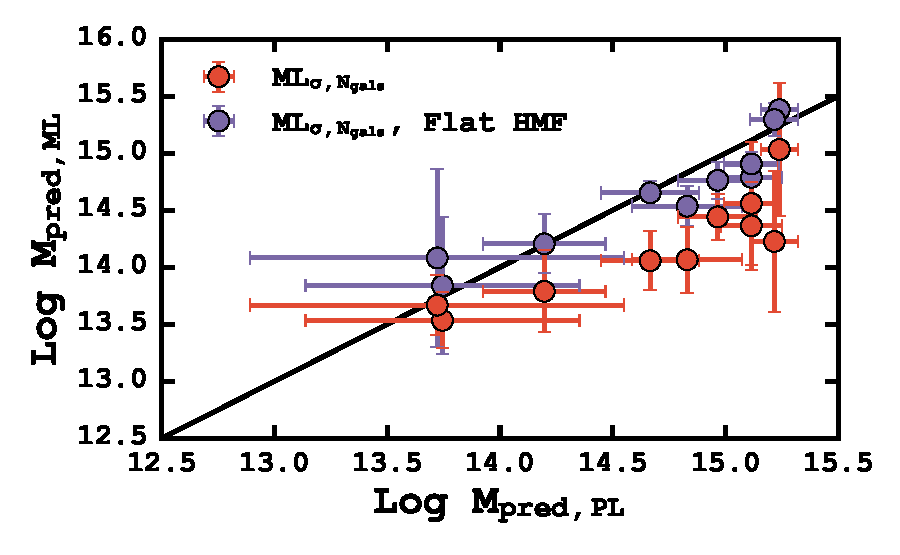
\includegraphics[width=0.6\textwidth]{figures2/massCompare.pdf} 
	\end{center}
	\caption[PL estimated cluster versus ML predicted cluster mass]{Comparison of the cluster mass estimates for the PL scaling relation (Equation~\ref{2eq:power law}) and the ML based mass predictions. We find the ML method sigificantly underestimates the cluster mass when compared to the PL method. This is due to the ML's reliance on training data which does not wholly represent the our sample of observed clusters.}
 \label{2fig: ML comparison} 
\end{figure}

In \citetalias{Boada2016} we find the ML based method with the LOSVD ($\sigma$), redshift ($z$) and number of galaxies observed ($N_{gal}$) showed both the smallest bias and scatter over the largest range of cluster masses. This worked well because the training data were selected from a volume of similar size to the survey in question. As discussed previously, we modify our analysis slightly and use the PL based approach (Eqn.~\ref{2eq:power law}) and the $\mathrm{ML}_{\sigma, N_{gal}}$ method to estimate the masses of our ten clusters. This change in the ML method is the result of the differences in the cosmological volume of the SDSS and the Buzzard at $z\sim2$.  

The PL predicted masses versus the ML predicted masses are shown in Figure~\ref{2fig: ML comparison}. We find that the PL based mass estimates are significantly higher than the ML based predictions, due to the ML relying on the biased training set discussed previously. In \citetalias{Boada2016}, the cluster mass prediction process uses two steps. Firstly the cluster mass is predicted, and then the cluster mass is corrected by considering the bias and scatter of the training data. Here, we choose to not correct the cluster masses predicted by either method due to the dissimilarity between the training data and our observations. During our testing, we find that there are too few training clusters with masses $> 10^{15}$ \Msol\ to place reliable contraints on the bias and scatter. As we discuss below, these high mass cluster constitute the bulk of our sample. Because we are unable to provide these clusters, with bias corrections, we choose to not correct any cluster mass estimate, to facilitate consistency throughout. 

The lack of a bias correction does not strongly effect our analysis as we are primarily interested in the scatter of our cluster masses. The scatter is unaffected as the individual mass estimates are scaled up or down by a common factor.

% The prediction process uses two steps. Firstly, we use a method to predict the individual masses and secondly we correct those masses based on the results of the training data. The upper panel of Figure~\ref{2fig: ML comparison} shows the cluster mass predictions for the Buzzard catalog clusters using the PL and $\mathrm{ML}_{\sigma, N_{gal}}$ approaches. The black diagonal line shows the 1:1 relation. The lower panel of Figure~\ref{2fig: ML comparison} shows the fractional error
% \begin{equation}\label{2eq: fractional error}
% 	\epsilon = (M_{pred} - M_{200c})/M_{200c}
% \end{equation}
% as a function of true cluster mass, $M_{200c}$ from the simulation.
%
% Using the predicted cluster masses for the Buzzard catalog we can quantify the amount of bias, and the scatter about that bias for different bins of predicted cluster mass. The bias is correctable by simply shifting our predicted cluster mass up or down by the appropriate amount. The scatter estimates the overall mass scale uncertainty in each bin of predicted cluster mass. We report the uncertainties in our cluster mass estimates as the sum in quadrature of the either confidence interval of the PL method or the prediction interval from the ML method and the mass scale uncertainty discussed here.

\begin{landscape}
	\begin{table}
	\caption[Summary of derived cluster parameters.]{Summary of derived cluster parameters: Column 1: The cluster name; Column 2: The number of SDSS sources observed; Column 3: The number of $Q=0(1)$ sources; Column 4: The number of member galaxies; Column 5: The redshift of the cluster; Columns 6: The LOSVD; Column 7: The PL predicted cluster mass; Column 8: The ML predicted cluster mass.} 
	\begin{tabular}{lccccccc} 
		\hline 
		&&&&&& PL & ML \\
		Cluster & Sources & Q=0 (1) & Member & $z_{c}$ & $\sigma$ (\kms) & log $M_{pred}$ & log $M_{pred}$ \\
		(1) & (2) & (3) & (4) & (5) & (6) & (7) & (8) \\
		\hline \hline 
		VCSJ010455.4+000336.3 & 41 & 10 (10) & 15 & 0.2727$\pm{0.0029}$ & 1194$\pm{135}$ & 15.11$\pm{0.14}$ & 14.84$\pm{0.18}$ \\
		VCSJ133520.1+410004.1 & 67 & 35 (17) & 25 & 0.2310$\pm{0.0025}$ & 1314$\pm{91}$ & 15.24$\pm{0.08}$ & 14.71$\pm{0.47}$ \\
		VCSJ140102.0+025242.6 & 67 & 14 (30) & 16 & 0.2543$\pm{0.0035}$ & 1295$\pm{115}$ & 15.22$\pm{0.11}$ & 14.55$\pm{0.45}$ \\
		VCSJ153656.3+242431.6 & 37 & 14 (14) & 11 & 0.2255$\pm{0.0034}$ & 932$\pm{189}$ & 14.83$\pm{0.24}$ & 14.21$\pm{0.16}$ \\
		VCSJ164019.8+464241.5 & 61 & 36 (14) & 32 & 0.2274$\pm{0.0020}$ & 1183$\pm{121}$ & 15.11$\pm{0.12}$ & 14.96$\pm{0.23}$ \\
		VCSJ172227.2+320757.2 & 61 & 26 (18) & 23 & 0.2260$\pm{0.0022}$ & 1044$\pm{154}$ & 14.97$\pm{0.18}$ & 14.54$\pm{0.14}$ \\
		VCSJ211849.1+003337.3 & 45 & 21 (8) & 18 & 0.2750$\pm{0.0026}$ & 820$\pm{148}$ & 14.67$\pm{0.22}$ & 14.30$\pm{0.12}$ \\
		VCSJ215422.9+003723.5 & 28 & 19 (2) & 16 & 0.2167$\pm{0.0026}$ & 547$\pm{124}$ & 14.20$\pm{0.27}$ & 14.04$\pm{0.09}$ \\
		XMMXCSJ124425.9+164758.0 & 25 & 11 (8) & 6 & 0.2316$\pm{0.0033}$ & 375$\pm{191}$ & 13.75$\pm{0.61}$ & 13.60$\pm{0.14}$ \\
		XMMXCSJ125650.2+254803.2 & 15 & 8 (3) & 3 & 0.2821$\pm{0.0059}$ & 372$\pm{258}$ & 13.72$\pm{0.83}$ & 13.52$\pm{0.13}$ \\
		\hline 
		\end{tabular}
		\label{2tbl: derived parameters} 
	\end{table}
\end{landscape}

Table~\ref{2tbl: derived parameters} presents a summary of the derived parameters for each cluster. We include the LOSVD, the estimated cluster redshift, and the number of member galaxies observed. We provide two predicted cluster masses, the PL based cluster mass and the $ML_{\sigma, N_{gal}}$ predicted cluster mass. We discuss the accuracy of both of these predictions in the following subsections.

\subsection{Notes for Individual Clusters}
Here we compare our PL inferred masses for the clusters in our sample to the previously reported estimates from the literature. \cite{Sifon2015} report total cluster masses for four of our clusters based on LOSVD measured from targeted spectra obtained with the Canada-France-Hawaii Telescope. They convert the LOSVD into a dynamical cluster mass using the PL scaling relation of \cite{Evrard2008} (which is the basis of our Equation~\ref{2eq:power law}) and estimate the uncertainties using jackknife resampling. One of our clusters has a reported LOSVD measurement and two have X-ray temperature measurements. In the following section we will discuss the ML estimated masses.

\subsubsection{VCSJ133520.1+410004.1 (Abell 1763)}
\cite{Sifon2015} observe 103 member galaxies within $r_{200}$. The compute a LOSVD of 1130$\pm81$ \kms, compared to our 1314$\pm91$ \kms\ based on 25 member galaxies. They report a $M_{200c} = (14.6\pm3.1) \times 10^14$ \Msol, compared to our value of $M_{200c} = (17.4\pm3.2) \times 10^14$ \Msol. The two estimates are consistent within the given errors, and the difference is due to our higher measured LOSVD.

\subsubsection{VCSJ140102.0+025242.6 (Abell 1835)}
\cite{Sifon2015} report a $M_{200c} = (4.5\pm1.9) \times 10^14$ \Msol, based on 41 member galaxies within
$r_{200c}$. We estimate a significantly different mass of $M_{200c} = (16.6\pm4.2)\times 10^{14}$ \Msol.
This discrepancy is due to the large difference in measured LOSVD, 762$\pm106$ \kms\ versus our
1295$\pm115$ \kms. However, \cite{Hoekstra2012} report a LOSVD for VCSJ140102.0+025242.6 of 1218 \kms.
\cite{Geller2013} find $M_{200c} = (16.57\pm1.86)\times 10^{14}$ \Msol\ from the best fitting caustic mass
profiles, which is similar to our reported value. Using \emph{Chandra} X-ray observations,
\cite{Bonamente2012} report a $M_{200c} = (8.35$\err{0.86}{0.81}$)\times 10^{14}$ \Msol. While our cluster
mass estimate is not consistent with \cite{Sifon2015}, we find it is very similar to other reported mass
estimates based on virial techniques.

\subsubsection{VCSJ164019.8+464241.5 (Abell 2219)}
With the largest number of member galaxies observed (of our sample), \cite{Sifon2015} use 241 member galaxies within $r_{200c}$ to estimate a mass of $M_{200c} = (17.0\pm2.8)\times 10^{14}$ \Msol. We estimate $M_{200c} = (12.9\pm3.6)\times 10^{14}$ \Msol. Using weak lensing techniques, \cite{Applegate2014} report a mass of $(12.0$\err{1.5}{1.5}$)\times 10^{14}$ \Msol\ within 1.5 Mpc, similar to our reported mass estimate.

\subsubsection{VCSJ172227.2+320757.2 (Abell 2261)}
For VCSJ172227.2+320757.2 we estimate $M_{200c} = (9.3\pm3.9)\times 10^{14}$ \Msol\ compared to $M_{200c} = (7.0\pm2.0)\times 10^{14}$ \Msol from \cite{Sifon2015}. They base their estimate on 76 member galaxies within $r_{200c}$. There is reasonable agreement between the two estimates.

\subsubsection{VCSJ215422.9+003723.5 (Abell 2392)}
The predicted mass of this cluster is significantly lower than expected. Previous work \citep{Wing2013} find it has a LOSVD of 1485 \kms\ well outside the estimated value from our analysis of $547\pm124$. \cite{Wing2013} report a LOSVD based on 32 member galaxies within 3 Mpc of the cluster center. One possible explanation for the deviation between our result and that of \cite{Wing2013} is that our observations probe only the cluster core ($<0.4$ Mpc), while their measurements include galaxies much farther away. Previous theoretical work \citeeg{Old2013} has shown the LOSVD to be sensitive to the radius at which it is measured. In addition, there is evidence to suggest that the cores of some galaxy clusters exhibit a smaller velocity dispersion than the outskirts \citeeg{Bahcall1977, Muriel2002}.

\subsubsection{XMMXCSJ124425.9+164758.0}
With only six member galaxies identified, XMMXCSJ124425.9+164758.0 is near the very limit of our ability to produce accurate cluster mass estimates. Fortunately, the cluster has an measured x-ray temperature which we can use to as another estimate of mass. Its XCS data release 1\footnote{http://www.astro.ljmu.ac.uk/$\sim$xcs/DR1/XCSDataRelease.html} \citep{Mehrtens2012} measured temperature is 1.3\err{0.3}{0.2} KeV which equates to $M_{500c}\approx(0.41\pm0.08)\times10^{14}$ \Msol\ using the $T_x$-M relationship for low-temperature systems of \cite{Finoguenov2001}.

We convert this X-ray inferred mass from $M_{500c}$ to $M_{200c}$ using the general prescription in \cite{Hu2003} to arrive at a predicted mass of $M_{200c} \approx (0.53\pm0.11)\times10^{14}$ \Msol, in very good agreement with our LOSVD predicted value of $M_{200c} \approx (0.59\pm0.81)\times10^{14}$ \Msol.

\subsubsection{XMMXCSJ125650.2+254803.2}
The three member galaxies identified in XMMXCSJ125650.2+254803.2 do not place a statistically strong constraint on the LOSVD predicted cluster mass. It too has a X-ray temperature measurement as part of XCS. Using the same approach as with XMMXCSJ124425.9+164758.0, a measured X-ray temperature of 1.4\err{0.3}{0.2} KeV gives a X-ray inferred cluster mass of $M_{200c} \approx 0.61\times10^{14}$ \Msol. This is about 26\% higher than our LOSVD derived cluster masses. 

\subsection{On the Accuracy of ML based Cluster masses}
Many of the cluster masses predicted using the ML approach are significantly different from both the PL based masses and the values found in the literature. Specifically, the largest differences are for the high mass clusters, and this can wholly be attributed to the training data used to inform the ML method (see the discussion in Subsection~\ref{2sec: training features}). 

In \citetalias{Boada2016} we found significantly reduced scatter in our mass predictions through the use of ML methods. We argue that the amount of scatter and cluster mass accuracy are reasonable estimates of those for a survey such as HETDEX. In large part, this is because the cosmic volume probed by HETDEX is of similar size to that simulated by Buzzard. However, the clusters observed for this work are selected from the SDSS which covers a much larger cosmological volume. The smaller simulated volume of Buzzard leads to the issue where the training data does not accurately represent the population of clusters in question.

Simply, Buzzard lacks the intermediate redshift, high-mass cluster, which influences the ML predictions of the cluster mass. Improvements in the accuracy of the ML method are possible by (re-)introducing the cluster redshift as a feature (see \citetalias{Boada2016} as an example), but that would require a training dataset that has the same area/depth as the dataset used for the observations, in this case, the SDSS.

The prediction intervals output by the ML method also show the effect of the mis-matched training sample. The ML prediction intervals are narrower than the PL-inferred confidence intervals for all clusters with masses below $10^{15}$ \Msol. This is due to an abundance of training clusters in this range. Above this, there are too few clusters to give reliable predictions and the prediction interval widens to reflect that situation.

It is important to note, that the cluster mass predictions from the ML methods are not a failure of the method. Based on the training data the algorithm has been exposed to, it has predicted cluster masses which closely resemble the observed features. Supervised ML shows incredible promise as a tool for future astrophysical investigations, but a deep understanding of how the input training data effects the target output is also required.

\subsection{Optical Richness-Mass Relation}
\begin{figure}
	\begin{center}
		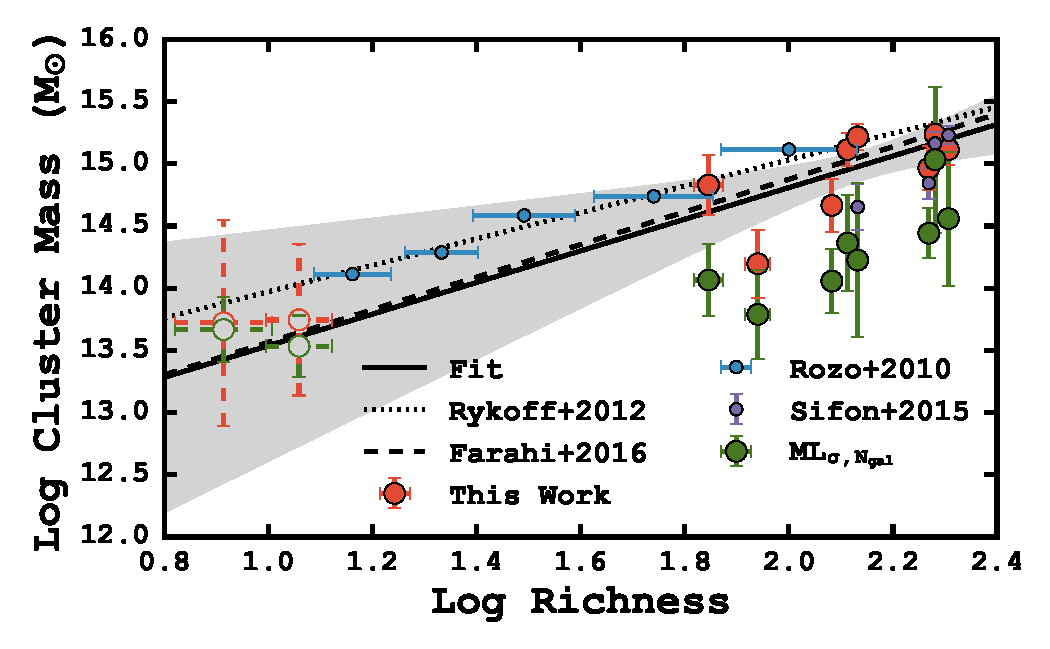
\includegraphics[width=\textwidth]{./figures2/massRichness.pdf} 
	\end{center}
	\caption[Richness versus total cluster mass for the clusters in our sample]{Richness, $\lambda$, versus total cluster mass for the clusters in our sample, shown as orange points. The two dashed points are the X-ray selected clusters, and are excluded from the fit. The solid black like shows our best-fitting relation (Equation~\protect\ref{2eq: best fit}) based on the eight high mass clusters, the dashed line shows the relation from \protect\cite{Farahi2016}, and the dotted line shows the relation from \protect\cite{Rykoff2012}. The gray shaded region corresponds to the 68\% confidence area on our best-fit. We also include stacked WL masses from \protect\cite{Rozo2010} and the high-mass cluster mass estimates of \protect\cite{Sifon2015} for comparison.}
\label{2fig:massRichness} 
\end{figure}

In \citetalias{Boada2016}, we show that HETDEX will be able to accurately estimate the absolute calibration and intrinsic scatter, $\sigma_{M|\lambda}$, of the optical-richness-cluster-mass relationship for a small range of intrinsic scatters. Here we use the ten clusters observed to demonstrate the ability of IFU observations similar to HETDEX to make mass determinations and to use those masses to place constraints on the optical-richness-cluster-mass relation. For our cluster mass estimates we use the masses predicted by the PL relation given in Equation~\ref{2eq:power law}. 

To find a best-fitting richness-mass relation for our data we are required to fit $y=mx+b$ where $y =$ log predicted cluster mass and $x =$ log optical richness, considering measurement errors in richness and predicted cluster mass along with intrinsic scatter of the relation. We assume the intrinsic scatter is constant from point to point, and we assume (not necessarily correctly) that all measurement errors are Gaussian. With the assumption of all Gaussian scatters we have three quantities of interest:
The probability of the predicted log cluster mass ($y_i$) given the observed log richness ($x_i$),
\begin{equation}\label{2eqn:intrinsic scatter}
	p(y_i|x_i) = \frac{1}{\sqrt{2\,\pi\,\sigma^2}}
	 \,\exp\left(-\frac{[y_i - m\,x_i - b]^2}{2\,\sigma^2}\right)
\end{equation}
which takes into consideration the intrinsic scatter in the relation, $\sigma$; the probability of the true log richness value ($\hat{x_i}$) given an observed log richness ($x_i$),
\begin{equation}\label{2eqn:xerr}
	p(\hat{x_i}|x_i) = \frac{1}{\sqrt{2\,\pi\,\sigma_{x,i}^2}}
	 \,\exp\left(-\frac{[\hat{x_i} - x_i]^2}{2\,\sigma_{x,i}^2}\right)
\end{equation}
which accounts for the uncertainty in the richness observation, $\sigma_{x,i}$; and the probability of the true log cluster mass ($\hat{y_i}$) given an observed log cluster mass ($y_i$),
\begin{equation}\label{2eqn:yerr}
	p(\hat{y_i}|y_i) = \frac{1}{\sqrt{2\,\pi\,\sigma_{y,i}^2}}
	 \,\exp\left(-\frac{[\hat{y_i} -y_i]^2}{2\,\sigma_{y,i}^2}\right)
\end{equation}
which also considers the uncertainty associated with the log cluster mass prediction, $\sigma_{y,i}$. We combine these three probabilities into
\begin{equation}
	p(\hat{y_i}|\hat{x_i}) = \int_{-\infty}^\infty dy_ip(\hat{y_i}|y_i) \int_{-\infty}^\infty dx_ip(y_i|x_i)p(x_i|\hat{x_i}).
\end{equation}
We assume flat priors on $x_i$ so that $p(x_i|\hat{x_i}) = p(\hat{x_i}|x_i)$ and substitute our probability equations from above. This gives
\begin{equation}
	p(\hat{y_i}|\hat{x_i}) = 
	\frac{1}{\sqrt{2\,\pi\,(\sigma^2 + \sigma_{y,i}^2 + m^2\sigma_{x,i}^2)}}\exp\left(-\frac{[y_i - m\,x_i - b]^2}{2\,(\sigma^2 + \sigma_{y,i}^2 + m^2\sigma_{x,i}^2)}\right)
\end{equation}
which for $\sigma_{x,i}=0$ (no uncertainty on the log richness measurement) reduces to the familiar form of a Gaussian with a combination of measurement error and intrinsic scatter. We convert this probability function into a likelihood by taking the product of all the individual probabilities,  
\begin{equation}\label{2eq:like}
\mathscr{L} = \prod_{i=1}^N \ p(\hat{y_i}|\hat{x_i}).
\end{equation}
and maximize this likelihood by sampling from the posterior probability distribution using the MCMC methods described above. We quote the most probable slope and intercept as the mean value of the posterior probability distributions with uncertainties as the square root of the second moment of the same distribution.

To find our best-fitting relation we exclude the two \emph{XMM} selected clusters due to the few number of observed member galaxies. After fitting to the remaining eight, high richness clusters, we find a best-fitting relation of 
\begin{equation}\label{2eq: best fit}
 \mathrm{Log}\,M_{200c}=1.25\pm{0.78}\, \mathrm{Log}\,\lambda + 12.29\pm{1.68}. 
\end{equation}
This best-fitting relation is shown in Figure~\ref{2fig:massRichness} where the large filled, orange points are the PL estimated cluster masses from this work, and the dashed points are the excluded \emph{XMM} selected clusters. We comment on the properties of our optical richness-mass relation and compare it to others from the literature in the following subsection.

We estimate the intrinsic scatter, $\sigma_{M|\lambda}$, in the relation two ways. The first is through our generative model, as it includes an intrinsic scatter term, which the MCMC samples directly. This gives $\sigma_{M|\lambda} = 0.23\pm0.16$ dex for the intrinsic scatter. We can also calculate the standard deviation of the residuals to the best-fitting line, which produces $\sigma_{M|\lambda} = 0.27\pm0.07$ dex. Both of these scatter estimates include the eight $\lambda > 60$ clusters. If we exclude VCSJ215422.9+003723.5 where we significantly underestimate the mass, the scatter for remaining seven clusters is $\sigma_{M|\lambda} = 0.24\pm0.09$ dex.

\subsection{Calibration of the Richness-Mass Relation}
We begin with a brief discussion of our best-fitting richness-mass relation. Two recent studies \citep{Farahi2016, Simet2016} use stacked cluster observations of velocity dispersions or WL, and it both cases report a PL index of $\alpha\sim1.33$. We find a similar (6\% difference) PL index of $\alpha\sim1.25$, albeit with significant uncertainty. Our absolute mass scale of log $M_{200c}/\Msol = 14.29\pm2.1$ dex at $\lambda=40$ is in good agreement with the previously reported values of log $M_{200c}/\Msol \sim 14.29$ dex, although with much greater uncertainty. These large uncertainties are due to our sample having so few reliable cluster mass estimates; our fitting procedure cannot place tight constraints on the measured slope and intercept. With the many clusters expected to be observed with HETDEX these uncertainties should decrease significantly.

% We begin with a brief discussion of the richness-mass relation itself. Because we have selected our clusters from the redMaPPer catalog, we begin with the richness-mass relation from \cite{Rykoff2012}. The authors suggest a PL index of $\alpha=1.06$ and an absolute mass scale of Log $M_{200c}/\Msol=14.64$ at $\lambda=60$. We find a 16\% difference in the slope, and a lower absolute mass scale of Log $M_{200c}/\Msol = 14.57\pm1.07$. \cite{Rykoff2012} go on to note that their relationship is not rigorously measured, so this discrepancy is unsurprising.

The individually measures cluster masses allow us to place promising constraints on the scatter in cluster mass at fixed richness, $\sigma_{M|\lambda}$. Using the SZE, \cite{Saro2015} find $\sigma_{M|\lambda} \sim 0.18$ at $\lambda = 70$. \cite{Rykoff2016} identify a similar scatter of $0.3\pm0.15$ using X-ray scaling relations and the DES science verification dataset. Many other studies \citeeg{Baxter2016, Farahi2016, Simet2016} adopt a $\sigma_{M|\lambda}\sim 0.2-0.3$ dex \citep{Rozo2014, Rozo2015}. These values correspond well to our value of $\sigma_{M|\lambda} = 0.24\pm0.09$ dex, and the $0.2-0.3$ range corresponds well to the region most sensitively probed in our simulated HETDEX survey \citepalias{Boada2016}.

The ability of blind spectroscopy to constrain both the absolute cluster mass scale and, more importantly, the amount of scatter at fixed optical richness to values similar to other techniques is extremely positive for the potential of HETDEX. As cluster mass estimates become better constrained through the use of ML methods, we can expect to find even tighter constrains on the optical richness-cluster mass relation. This should lead to excellent calibration of other large-area sky surveys which produce optical photometry only. In addition, it will serve as an important, independent check on other observable-cluster mass relationships which are often noisy and subjet to large systematic uncertainties \citeeg{Sereno2015}.

\section{Summary}\label{2sec:summary}
We carry out a proof-of-concept study where we present integral field unit observations with the Mitchelle Spectrograph of ten intermediate redshift ($z=0.2-0.3$) galaxy clusters. We observe cluster member galaxies within $R\sim0.5$ Mpc of each cluster, and determine each cluster's membership based on the line-of-sight velocity of each galaxy. The mass of each cluster is determined through a traditional PL and through a machine learning based approach. We use these estimates of cluster mass to measure the absolute mass scale and intrinsic scatter of the optical richness-cluster mass relationship. The goal of this study is to investigate how a blind spectroscopic survey, such as the forthcoming Hobby Eberly Dark Energy Experiment (HETDEX), will be able to predict cluster masses, and then to use those masses to help calibrate other observable-cluster mass scaling relations.
Our main results are as follows:
\begin{itemize}
	\item Using a PL scaling relation between the measured line-of-sight velocity dispersion and cluster mass, our low richness ($\lambda < 15$) sample of galaxy clusters have total inferred masses $\sim 0.5 \times 10^{14}$ \Msol\ ($M_{200c}$), and the high richness ($\lambda > 60$) cluster sample has total masses $(1.58-17.37) \times 10^{14}$ \Msol\ ($M_{200c}$). The majority of these estimate are consistent with other published total mass estimates which use a variety of estimation techniques. 
	
	\item The machine learning based approach of galaxy cluster mass estimation, while powerful, requires a deep understanding of both the machine learning algorithms available, and expert knowledge of the problem domain. To estimate the total masses of the galaxy clusters in our sample using machine learning methods, the Buzzard catalogs do not provide a suitable training set due to the limited cosmological volume simulated at low redshift. For the redshift range of our cluster sample, the Buzzard catalogs lack similar high velocity dispersion clusters. This leads to a severe down-weighting of high mass galaxy clusters when the cluster redshift is included as a training feature. When this feature is removed, the machine learning estimated cluster masses improve but are still underestimated due to too few very high mass clusters being included in the simulated volume. A suit a training data drawn from a similarly sized cosmological volume is critical to the reliable prediction of cluster masses. When this is available, the machine learning predicted cluster masses show less bias and lower scatter compared to a traditional power law scaling relation based on velocity dispersion alone.

	\item We fit a optical richness-cluster mass relation to the eight high richness ($\lambda > 60$) clusters. This gives:
		\begin{equation}
			\mathrm{Log}\,M_{200c}=1.25\pm{0.78}\, \mathrm{Log}\,\lambda + 12.29\pm{1.68}.  
		\end{equation}
We are unable to place tight constraints on the overall estimate of the normalization due to the relatively few clusters included. We do estimate the scatter in cluster mass at fixed richness, $\sigma_{M|\lambda} \sim 0.25$. This estimate of scatter compares well with other recent studies of the richness-mass relation. This suggests that a blind spectroscopic survey such as HETDEX will be able to provide a crucial, independent measurement of this scatter, to a much high precision than is possible in this work. This bodes well for the success of HETDEX as not only a high redshift galaxy survey but as a important calibration tool for understanding the uncertainties associated with galaxy cluster mass estimates. 
\end{itemize}

%%%%%%%%%%%%%%%%%%%%%%%%%%%%%%%%%%%%%%%%%%%%%%%%%%%
%
%  New template code for TAMU Theses and Dissertations starting Fall 2012.  
%  For more info about this template or the 
%  TAMU LaTeX User's Group, see http://www.howdy.me/.
%
%  Author: Wendy Lynn Turner 
%	 Version 1.0 
%  Last updated 8/5/2012
%
%%%%%%%%%%%%%%%%%%%%%%%%%%%%%%%%%%%%%%%%%%%%%%%%%%%

%%%%%%%%%%%%%%%%%%%%%%%%%%%%%%%%%%%%%%%%%%%%%%%%%%%%%%%%%%%%%%%%%%%%%%%
%%%                           SECTION I
%%%%%%%%%%%%%%%%%%%%%%%%%%%%%%%%%%%%%%%%%%%%%%%%%%%%%%%%%%%%%%%%%%%%%%

\renewcommand*{\thefootnote}{\fnsymbol{footnote}}
\chapter[\uppercase{A pilot survey to measure Cluster Dynamics: Targeted Observations with the VIRUS Prototype Instrument}]{\uppercase{A pilot survey to measure Cluster Dynamics: Targeted Observations with the VIRUS Prototype Instrument}}% \symbolfootnote[1]{Reprinted with permission from ``Introduction: The Importance of Research'' by AUTHOR et al., 2015. The Astrophysical Journal, Volume XYZ, Issue X, article id. XY, XY pp., Copyright 20XX by the American Astronomical Society.} }
% \renewcommand*{\thefootnote}{\arabic{footnote}}
\setcounter{footnote}{0}

\section{Introduction} 
Many large area-sky surveys both currently underway and upcoming are prioritizing the identification of clusters for both detailed studies of cosmology and for fundamental physical examinations of galaxy properties in rich environments. At present, the greatest number of clusters are being identified using large millimeter wave surveys with the South Pole Telescope (SPT; \citealt{Carlstrom2011}) or the Atacama Cosmology Telescope (ACT; \citealt{Swetz2011}). These observations rely on the Sunyaev-Zel'dovich effect (SZE; \citealt{Sunyaev1972}) which uses the up-scattering of cosmic microwave background (CMB) photons to both identify the cluster and to estimate its mass. X-ray surveys of cluster \citeeg{Voges1999, Bhringer2001, Mehrtens2012} continue to play an important role, which will continue to increase as future large-area X-ray surveys (\eg, eROSITA \citealt{Merloni2012}) become available. However, deep, wide field optical surveys, such as the Dark Energy Survey (DES; \citealt{DES2005}) and planned Large Synoptic Survey Telescope (LSST; \citealt{LSST2012}) will discover many more clusters at increasing lower mass in the near future; at its completion, DES is expected to identify approximately 100,000 clusters at $z<1$ \citep{DarkEnergySurveyCollaboration2016}, of which about 1000 clusters with SZE and X-ray observations currently overlap with DES identified clusters. Such surveys will employ the richness of the individual clusters as a cluster mass proxy, and as such, will rely on follow-up observations to better constrain the absolute scale and the scatter in the richness-mass relation. But, as the number of clusters grows to many tens of thousands, individual spectroscopic confirmation becomes unfeasible. Therefore, we rely on well calibrated observable-mass relationships to estimate the masses of the observed clusters.

Unfortunately, mass is not directly observable, so we must estimate it through another discernible cluster property. Observed X-ray temperatures and luminosities correlate tightly with a cluster's dynamical mass \citeeg{Mantz2010, Rykoff2014}, especially for dynamically relaxed clusters \citeeg{Mantz2015}. Observations of the SZE provide accurate estimations of mass \citeeg{Vanderlinde2010, Sehgal2011}, but can be effected by the physics of the intracluster medium \citeeg{Pipino2010} and the ability to detect low mass galaxy clusters is currently limited by technology \citeeg{Carlstrom2002a}. The richness \citeeg{Abell1958,Rykoff2012} is, at present, defined to be the weighted number of cluster member galaxies with a scale aperture. It has been shown to correlate strongly with cluster mass in the mean \citeeg{Rozo2010}, providing a powerful cluster mass estimate based on photometry alone.

The richness is already being used in many optical studies \citeeg{Ruel2014, Sifon2015}, but the absolute mass scale and more importantly the intrinsic scatter in the relation are currently under active investigation \citeeg{Rozo2015, Saro2015, Baxter2016, Farahi2016, Rykoff2016, Simet2016}. \cite{Saro2015} find their estimates of the intrinsic scatter is not dominated by the SZE-mass scaling relation, and can be substantially improved with a larger sample of clusters. These systematics remain the major source of uncertainty in deriving cosmological constraints from cluster abundances and testing structure growth in a $\Lambda$CDM universe. The intrinsic scatter in the richness-mass relation has been estimated to be approximately 20\% \citep{Saro2015, Rykoff2016}. To realize fully the promise of the large samples from DES and LSST, we must measure both the absolute mass scale and scatter in the optical-richness mass estimator using independent methods.

The Hobby Eberly Dark Energy Experiment (HETDEX; \citealt{Hill2008}) is a forthcoming blind spectroscopic survey that offers the ability to calibrate accurately the optical richness-mass relation for a significant number of galaxy clusters at both extremes of the mass scale. At present, because HETDEX is designed to measure the dark energy equation of state at $z\sim0.2$, and the applicability to galaxy cluster science has not yet been investigated.  We began this investigation in Section 2. The blind spectroscopic observations of HETDEX are capable of accurately estimating galaxy cluster masses over the range of redshifts and cluster masses covered by the study. Using a machine learning approach where several cluster observables are combined, we estimate cluster masses to a similar level of precision as a fully targeted survey. The ability of HETDEX to further constrain optically derived masses is of paramount importance to upcoming large photometric surveys. This study provides insight into how well a HETDEX type survey will constrain mass estimations and cosmological parameters in the future.

In this section, we present a pilot study of ten massive galaxy clusters using integral field spectroscopy with the Mitchell Spectrograph as a pilot program for HETDEX. The goal of this study is to obtain spectroscopic redshifts of the individual cluster galaxies, determine the velocity dispersion and to infer each cluster's dynamical mass. This allows us to compare the inferred mass with other mass estimators (\eg, the clusters in this sample have deep \textit{Chandra} or \textit{XMM-Newton} X-ray data, and richness measurements) with the aim of better characterizing the scatter in the richness-mass relation, $\sigma_{M|\lambda}$.

The layout of this section is the following. In Section~\ref{2sec:design} we discuss the target selection and the setup of the Mitchell Spectrograph used to conduct the observations. Section~\ref{2sec:data reduction} describes the methods and tools used to reduce the observations. We present our redshift catalog, cluster members and cluster dynamical properties in Section~\ref{2sec:analysis}. We discuss a machine learning based alternative to a traditional power law estimate of cluster mass in Section~\ref{2sec:ML methods} In Section~\ref{2sec:results}, we compare and discuss the different mass estimations and remark on the applicability of these methods for the study of the optical richness-cluster mass relationship.  Finally, we summarize this work in Section~\ref{sec:summary}.

Throughout this section, we adopt the following cosmological model from the Buzzard simulations (see Section~\ref{2sec:ML methods}): $\Omega_\Lambda = 0.714$, $\Omega_M = 0.286$, and $H_0= 70$ \kms \mpc, assume a Chabrier initial mass function (IMF; \citealt{Chabrier2003}), and use AB magnitudes \citep{Oke1974}.

\section{Design}\label{2sec:design} 
\subsection{Target Selection}\label{2sec:selection} 
We select clusters at $z=0.2-0.3$ using two different methods and for two different purposes. We optically select eight of the ten clusters from \cite{Rykoff2012} using the \textit{Sloan Digital Sky Survey} (SDSS; \citealt{Blanton2001a}) Data Release 8. These clusters have high ($\lambda>70$) observed richnesses which corresponds to $M > 2.2\times10^{14}$ \Msol, and are a combination of relaxed and unrelaxed systems. The last two clusters are selected from the \textit{XMM Cluster Survey} (XCS; \citealt{Mehrtens2012}) and correspond to individually measured X-ray temperatures of $T_X < 2.5$ keV. Such X-ray temperatures have inferred masses of $10^{14}\msol > M_{DM} > 5\times10^{13}\Msol$.

The optically selected clusters have many more members, by up to a factor of 8, (see Table~\ref{2tbl:targets}) than the X-ray selected clusters which allows us to investigate the accuracy of our mass recovery methods at both cluster and group scales. See Table~\ref{2tbl:targets} for individual cluster sky positions and associated parameters. 

\begin{landscape}
	\begin{table}
	\caption[Basic properties of the ten galaxy clusters targeted with the MS.]{Basic properties of the ten galaxy clusters targeted with the MS: Column 1: Our internal cluster name; Column 2: Abell Catalog ID; Column 3: The right ascension of the cluster; Column 4: The declination of the cluster; Column 5: the nominal (often photometric) cluster redshift; Column 6: The measured richness from \cite{Rykoff2012}; Column 7: The date of our observations.}
	\begin{centering} 
	\begin{tabular}{lcccccc} 
		\hline 
		Cluster & Abell ID & RA (J2000) & DEC (J2000) & $z$ & $\lambda$ & Obs. Date\\
		(1) & (2) & (3) & (4) & (5) & (6) & (7) \\
		\hline \hline
		MSJ010455.4+000336.3 & \nd & 01:04:55.369 & +00:03:36.28 & 0.277 & $129.7\pm4.9$ & August, 2012 \\
		MSJ133520.1+410004.1 & Abell 1763 & 13:35:20.092 & +41:00:04.12 & 0.223 & $191.0\pm5.7$ & May, 2012 \\
		MSJ140102.0+025242.6 & Abell 1835 & 14:01:01.965 & +02:52:42.63 & 0.252 & $135.6\pm5.2$ & May, 2012 \\
		MSJ153656.3+242431.6 & \nd & 15:36:56.253 & +24:24:31.60 & 0.226 & $70.1\pm4.4$ & May, 2012 \\ 
		MSJ164019.8+464241.5 & Abell 2219 & 16:40:19.812 & +46:42:41.51 & 0.225 & $202.6\pm5.4$ & May, 2012 \\
		MSJ172227.2+320757.2 & Abell 2261 & 17:22:27.182 & +32:07:57.24 & 0.224 & $185.8\pm7.4$ & May, 2012 \\
		MSJ211849.1+003337.3 & \nd & 21:18:49.069 & +00:33:37.33 & 0.270 & $121.0\pm4.6$ & August, 2012 \\
		MSJ215422.9+003723.5 & Abell 2392 & 21:54:22.936 & +00:37:23.48 & 0.223 & $87.2\pm4.8$ & August, 2012\\
		XMMXCSJ124425.9+164758.0 & \nd & 12:44:25.203 & +16:47:48.00 & 0.235 & $11.4\pm1.7$ & May, 2013 \\
		XMMXCSJ125650.2+254803.2 & \nd & 12:56:49.999 & +25:48:02.99 & 0.280 & $8.2\pm1.8$ & May, 2013 \\
		\hline 
		\end{tabular}
	\end{centering}
		\label{2tbl:targets} 
	\end{table}
\end{landscape}

\subsection{Observations} 
We use the Mitchell Spectrograph (MS; formerly known as VIRUS-P; \citealt{Hill2008a}) an integral field unit (IFU) in a square array of 246 $4\farcs24$ diameter optical fibers. This provides a $1\farcm7~\times~1\farcm7$ field-of-view (FOV) with a 1/3 filling factor. A Fairchild Instruments, 2k$\times$2k charge couple device (CCD) images the spectra from each of the 246 fibers. The spectra have approximately a gaussian profile with a 5 pixel full width at half maximum (FWHM), and each are separated by 8 pixels to minimize the amount of cross-talk between the fibers. 

There are two spectral configurations available on MS, a blue setup, 3600-5800 \AA\ and a red setup, 4600-6800 \AA. In addition, there are four volume phase holographic gratings available to disperse the light. For the purpose of this work, the lowest resolution, $\sim5$\AA, grating is used. At the native pixel scale, this translates into a spectral dispersion of $\sim1.11$ \AA\ pixel$^{-1}$. 

We use MS to target the galaxy clusters using the 5 \AAA\ grating covering a wavelength range of $4400 - 6600$ \AAA. With this instrumental setup and for galaxies $z = 0.2-0.3$, we will cover the Ca H\&K, Fe I ($\lambda 4383$), H-$\delta$, H-$\gamma$ and H-$\beta$ absorption features. Additionally, we cover emission of the [\ion{O}{II}] ($\lambda\lambda 3727,3729$) doublet, H-$\beta$, and [\ion{O}{III}] ($\lambda\lambda 4960,5008$), which allows for the identification of actively star-forming galaxies.

\begin{figure}[!ht]
	\begin{center}
		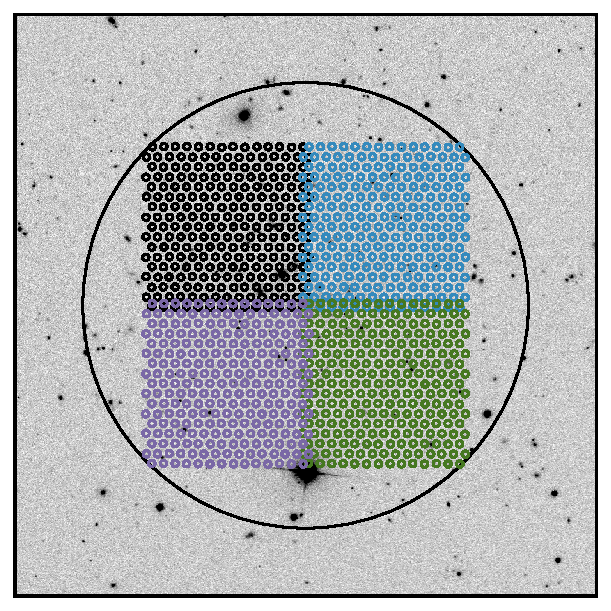
\includegraphics[width=\textwidth]{./figures2/pointing.pdf} 
	\end{center}
	\caption[SDSS \sdssr-band image of an optically selected galaxy cluster Abell 2631 selected from the SDSS DR8 data, centered on the BCG.]{SDSS \sdssr-band image of an optically selected galaxy cluster Abell 2631 ($z=0.273$) selected from the SDSS DR8 data, centered on the BCG. The large black circle shows the region $R<0.5$ Mpc ($r<2\farcm3$). The northeast (NE), northwest (NW), southwest (SW), and southeast (SE) fields with the fiber positions are shown in black, blue, green and purple respectively, illustrating how we survey each cluster. Nearly all galaxies within this region are associated with the cluster.}
	\label{2fig:tiles} 
\end{figure}

The FOV of the MS corresponds to an approximately 0.4 Mpc square region at $z = 0.2-0.3$. To ensure adequate coverage of the cluster out to a radius of 0.5 Mpc, we use four MS pointings per cluster. Figure~\ref{2fig:tiles} shows an example of the pointing pattern done on each cluster. The entire field is centered on the brightest cluster galaxy (BCG) and the individual tiles are shifted away. Furthermore, each of the four tiles are dithered at relative positions $(\Delta \alpha, \Delta \delta)=(0\farcs0,0\farcs0)$, $(-3\farcs6,-2\farcs0)$, and $(0\farcs0, -4\farcs0)$ from the origin to ensure full coverage of the FOV. Therefore, there are 736 individual spectra for each of the four fields or 2952 measurements for the cluster as a whole.

We have set exposure times to achieve spectra with signal-to-noise ratios (SNRs) $\sim3$ per spectral element (averaged over 4.6 pixels) in the continuum for objects with \sdssg\ $= 21.3$ mag (which corresponds to approximately 0.2L$^\star$ for cluster galaxies at $z = 0.2$) in 3600 seconds per pointing.. We base the expected SNR on the experience of \cite{Shetrone2010}, who achieves SNR $= 100$ per pixel in the continuum for point sources with B $=16.5$ mag at 4000 \AAA\ in 4800 seconds. Therefore, we require 1 hr/pointing $\times$ 4 pointings $= 4$ hrs on sky per cluster. Even though the field is dense with galaxies, there is sufficient ``blank'' area to allow for enough ``sky'' fibers for background subtraction.

\section{Data Reduction}\label{2sec:data reduction} 
All data are reduced using \textsc{p3d}\footnote{http://p3d.sourceforge.net/} \citep{Sandin2010} a general-use IFU reduction pipeline. The first step is to min/max-filtered average combine a minimum of 20 bias images from each night into a master-bias image, which is subtracted from each other image from the same night. Secondly, a trace mask is created from flat-fielding on the dusk or dawn sky. The fibers are fairly densely packed, so to determine the position of each spectrum in the dispersion direction each spectrum is extracted using a multi-profile deconvolution approach \citep{Sharp2010} to account for cross talk between fibers. Third, a dispersion mask for the wavelength calibration from images of Hg+Cd (for the May, 2012 observations) or Cd+Ne (for all other observations) arc lamps. The residuals between the derived wavelength solution and the known wavelengths of the emission lines is calculated from a fifth order polynomial and lie between $0.02 - 0.06$ \AAA. Finally, a fiber flat is created from the sky flats by a min/max-filtered average combine as in step one. 

We extracted the science spectra using several steps. First, we subtract the bias frames from each science frame. Next, we use \textsc{PyCosmic} \citep{Husemann2012}, integrated into \textsc{p3d} with the default parameters, to clean cosmic ray hits. Third, we use the previously created dispersion mask to wavelength calibrate the extracted spectra. Aligning the dispersion mask to bright telluric lines (namely \hbox{[\ion{O}{I}]} at 5577 \AAA) accounts for any flexure in the instrument between the images of the arc lamps and science frames. Finally, we normalize the extracted spectra using the transmission in the fiber flats from above. 

The result of this process is row-stacked spectra and associated pipeline-propagated uncertainties, where each of the 246 fibers are stored individually. A table of fiber positions maps each spectrum onto the image plane. However, for many of our observations a precise astrometric solution for the fiber positions is unknown due to an offset between the software which calculates the fiber positions and the telescope telemetry. To reconstruct accurate fiber positions we first identify fibers which observe stars and identify which fibers the astrometric solution indicates should contain stars. In many cases the stars are located between fibers. To account for this we use a simple Gaussian centroid weighted by the observed flux $5000 \leq \lambda \leq 5010$ \AAA\ to find the correct sky position of the star. We then shift the fiber grid to match the sky position of the stars as reported by the SDSS. For each observation we use as many stars as possible and combine the shifts to generate a mean offset. Typical shifts are $0\farcs5 - 4''$, less than the width of a single fiber. This offset is applied to all dithers of each observation. There is little need to obtain highly accurate fiber positions as the $4\farcs24$ fibers ensures that reasonably correct positions will identify which fibers contain galaxies.

We use a simple sky subtraction scheme to remove the majority of the sky contamination. Because the majority of fibers for any single pointing are empty, we use a $3\sigma$ clipped median of all spectra at each wavelength which removes fibers containing continua leaving only blank fibers. A simple mean combines the sky fibers into a single sky spectra. The result is then subtracted from every fiber. This adequately removes the bulk of sky emissions lines, but often fails to completely remove the [\ion{O}{I}] line at 5577~\AAA. Our inspection of the sky subtracted spectra shows residual [\ion{O}{I}] line flux approximately $10-15$\% of the un-sky subtracted level. We mask any emission line with a sky-subtraction residual $>10\%$ to ensure they have minimal effect.

\begin{figure}[t]
\subfloat{%
  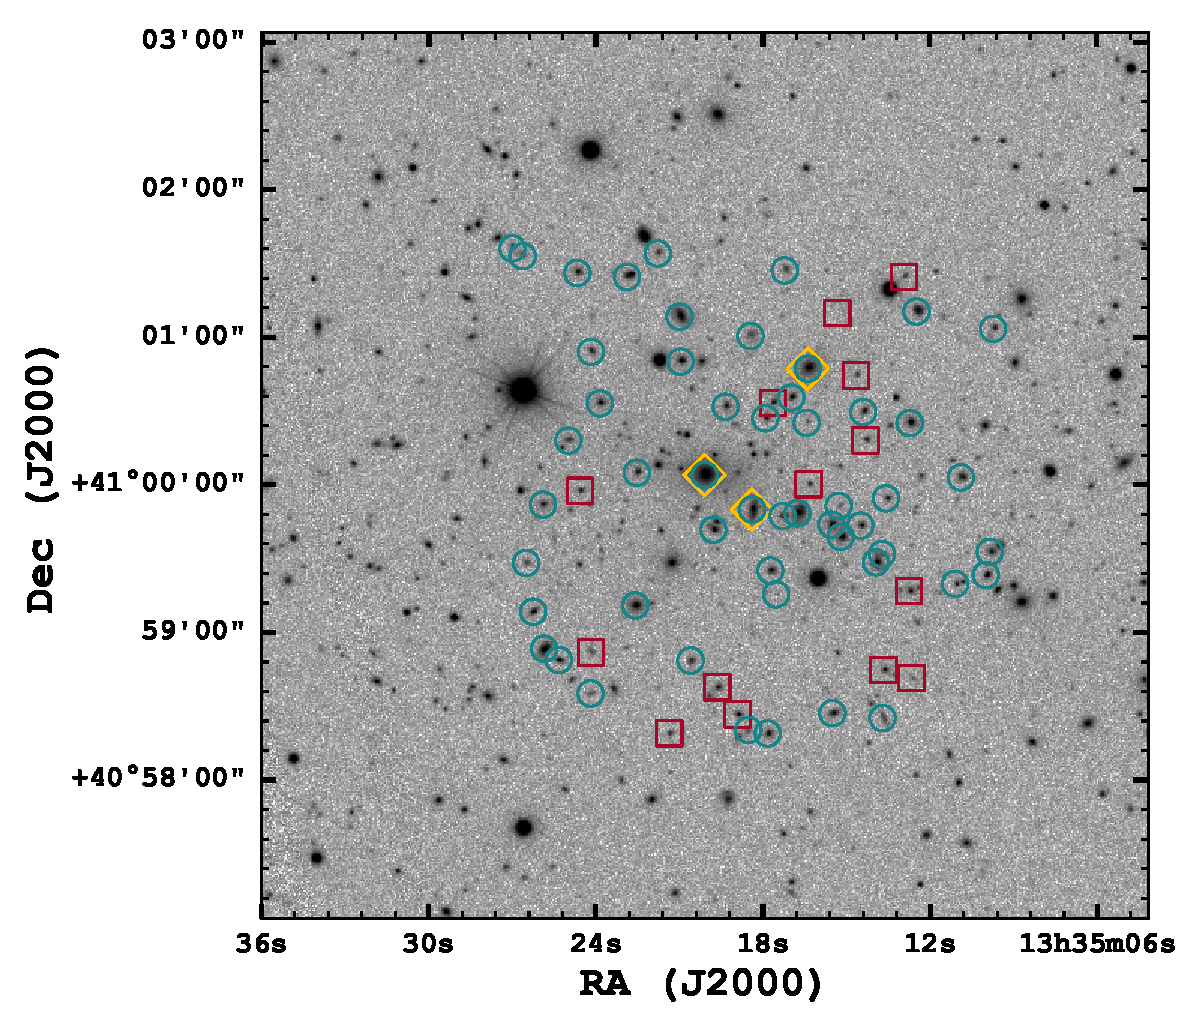
\includegraphics[width=0.5\textwidth]{./figures2/c203p83+41p0_mosaic.pdf}
}
\hfill
\subfloat{%
  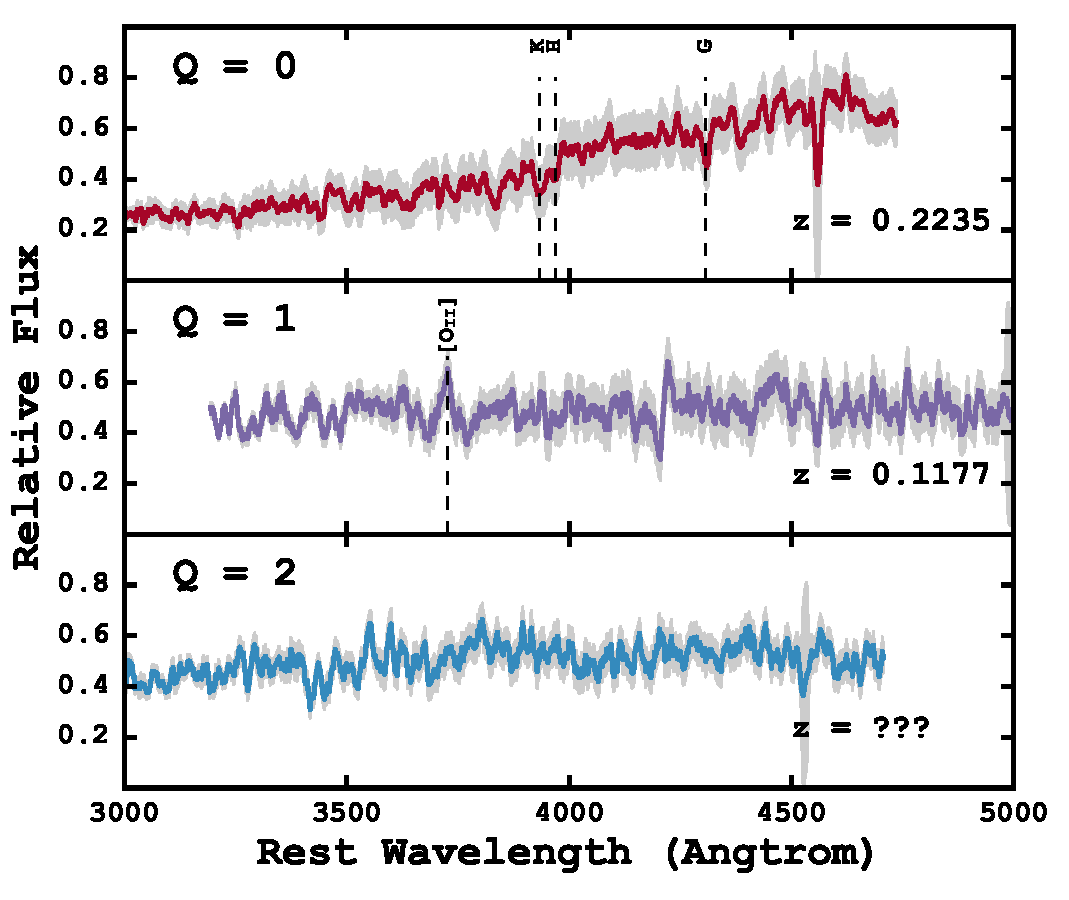
\includegraphics[width=0.5\textwidth]{./figures2/spectrum.pdf}
}
    \caption[SDSS \sdssr-band image of cluster MSJ133520.1+410004.1.]{SDSS \sdssr-band image of cluster MSJ133520.1+410004.1. The symbols show the position of observed galaxies. Turquoise circles indicate galaxies with $Q=0$ or $Q=1$ spectroscopic redshifts, red squares indicate galaxies where a redshift could not be reliably determined, and the yellow diamond corresponds to galaxies with pre-existing redshifts from the SDSS. \textit{Right:} Example spectra, with major features identified, showing the three quality flags. $Q=0$ represents the best quality spectra and $Q=2$ the poorest quality. Grey shaded regions show the {\sc p3d} internally estimated, relative errors. We take galaxies with $Q=0$ and $Q=1$ for the analysis in this study.} 
	\label{2fig:MSJ133520.1+410004.1}
\end{figure}

After reducing all spectra we find an average residual uncertainty in the wavelength solution of $\sigma_\lambda \sim 0.4$ \AAA\ or 24 \kms\ at 5000 \AAA, small compared to the instrumental resolution. We find an average instrumental resolution of $\sim144$ \kms, by fitting Gaussians to the observed emission lines in the calibration lamp images. Combining the two in quadrature gives a total instrumental resolution of $\sigma_{inst} = 146$ \kms, similar to that of other studies using the MS \citeeg{Murphy2011, Blanc2013}.

\section{Analysis}\label{2sec:analysis} 
The analysis of our reduced spectra occurs in two stages. First we derive individual redshifts using the observed spectra, and then utilize the redshifts collectively to identify which galaxies likely belong to the galaxy cluster.

Individual galaxy selection is done through cross matching the IFU fiber sky positions with galaxies selected from the SDSS. To collect the galaxies from the SDSS, we select all galaxies with $\sdssg <$ 22 mag within $3'$ of the BCG in each cluster. For each cluster we create catalogs of photometry in all SDSS bands (\sdssu\sdssg\sdssr\sdssi\sdssz), photometric redshift, and any spectroscopic redshift. The following SQL query accomplishes this task for MSJ010455.4+000336.3.
\begin{singlespace}
\begin{lstlisting}[language=SQL]
SELECT TOP 1000 G.objid, 
                G.ra, 
                G.dec, 
                G.u, 
                G.err_u, 
                G.g, 
                G.err_g, 
                G.r, 
                G.err_r, 
                G.i, 
                G.err_i, 
                G.z, 
                G.err_z, 
                Pz.z    AS Photoz, 
                Pz.zerr AS Photoz_err, 
                SO.specobjid, 
                SO.ra   AS Spec_ra, 
                SO.dec  AS Spec_dec, 
                SO.z    AS Specz, 
                SO.zerr AS Specz_err 
FROM   galaxy AS G 
       JOIN dbo.Fgetnearbyobjeq(16.2307083,0.0600917,3) AS GN 
         ON G.objid = GN.objid 
       LEFT JOIN photoz AS Pz 
              ON G.objid = Pz.objid 
       LEFT JOIN specobj AS SO 
              ON G.objid = SO.bestobjid 
WHERE  G.g < 22 
       AND clean = 1 
       AND ( calibstatus_r & 1 ) != 0
\end{lstlisting}
\end{singlespace}

Because of the large number of fiber pointings, only fibers which overlap within 4\farcs16 of an SDSS source are considered for redshift analysis. The left panel of Figure \ref{2fig:MSJ133520.1+410004.1} shows cluster MSJ133520.1+410004.1 with the SDSS detections and measured redshifts overlaid. Orange diamonds are galaxies with SDSS available redshifts. The blue circles and red squares correspond to galaxies where a redshift was and was not determined from the observed spectra. See Figure~\ref{2fig:multimontage} for a similar representation of the remaining nine clusters.

\begin{figure}[!ht]
	\begin{center}
		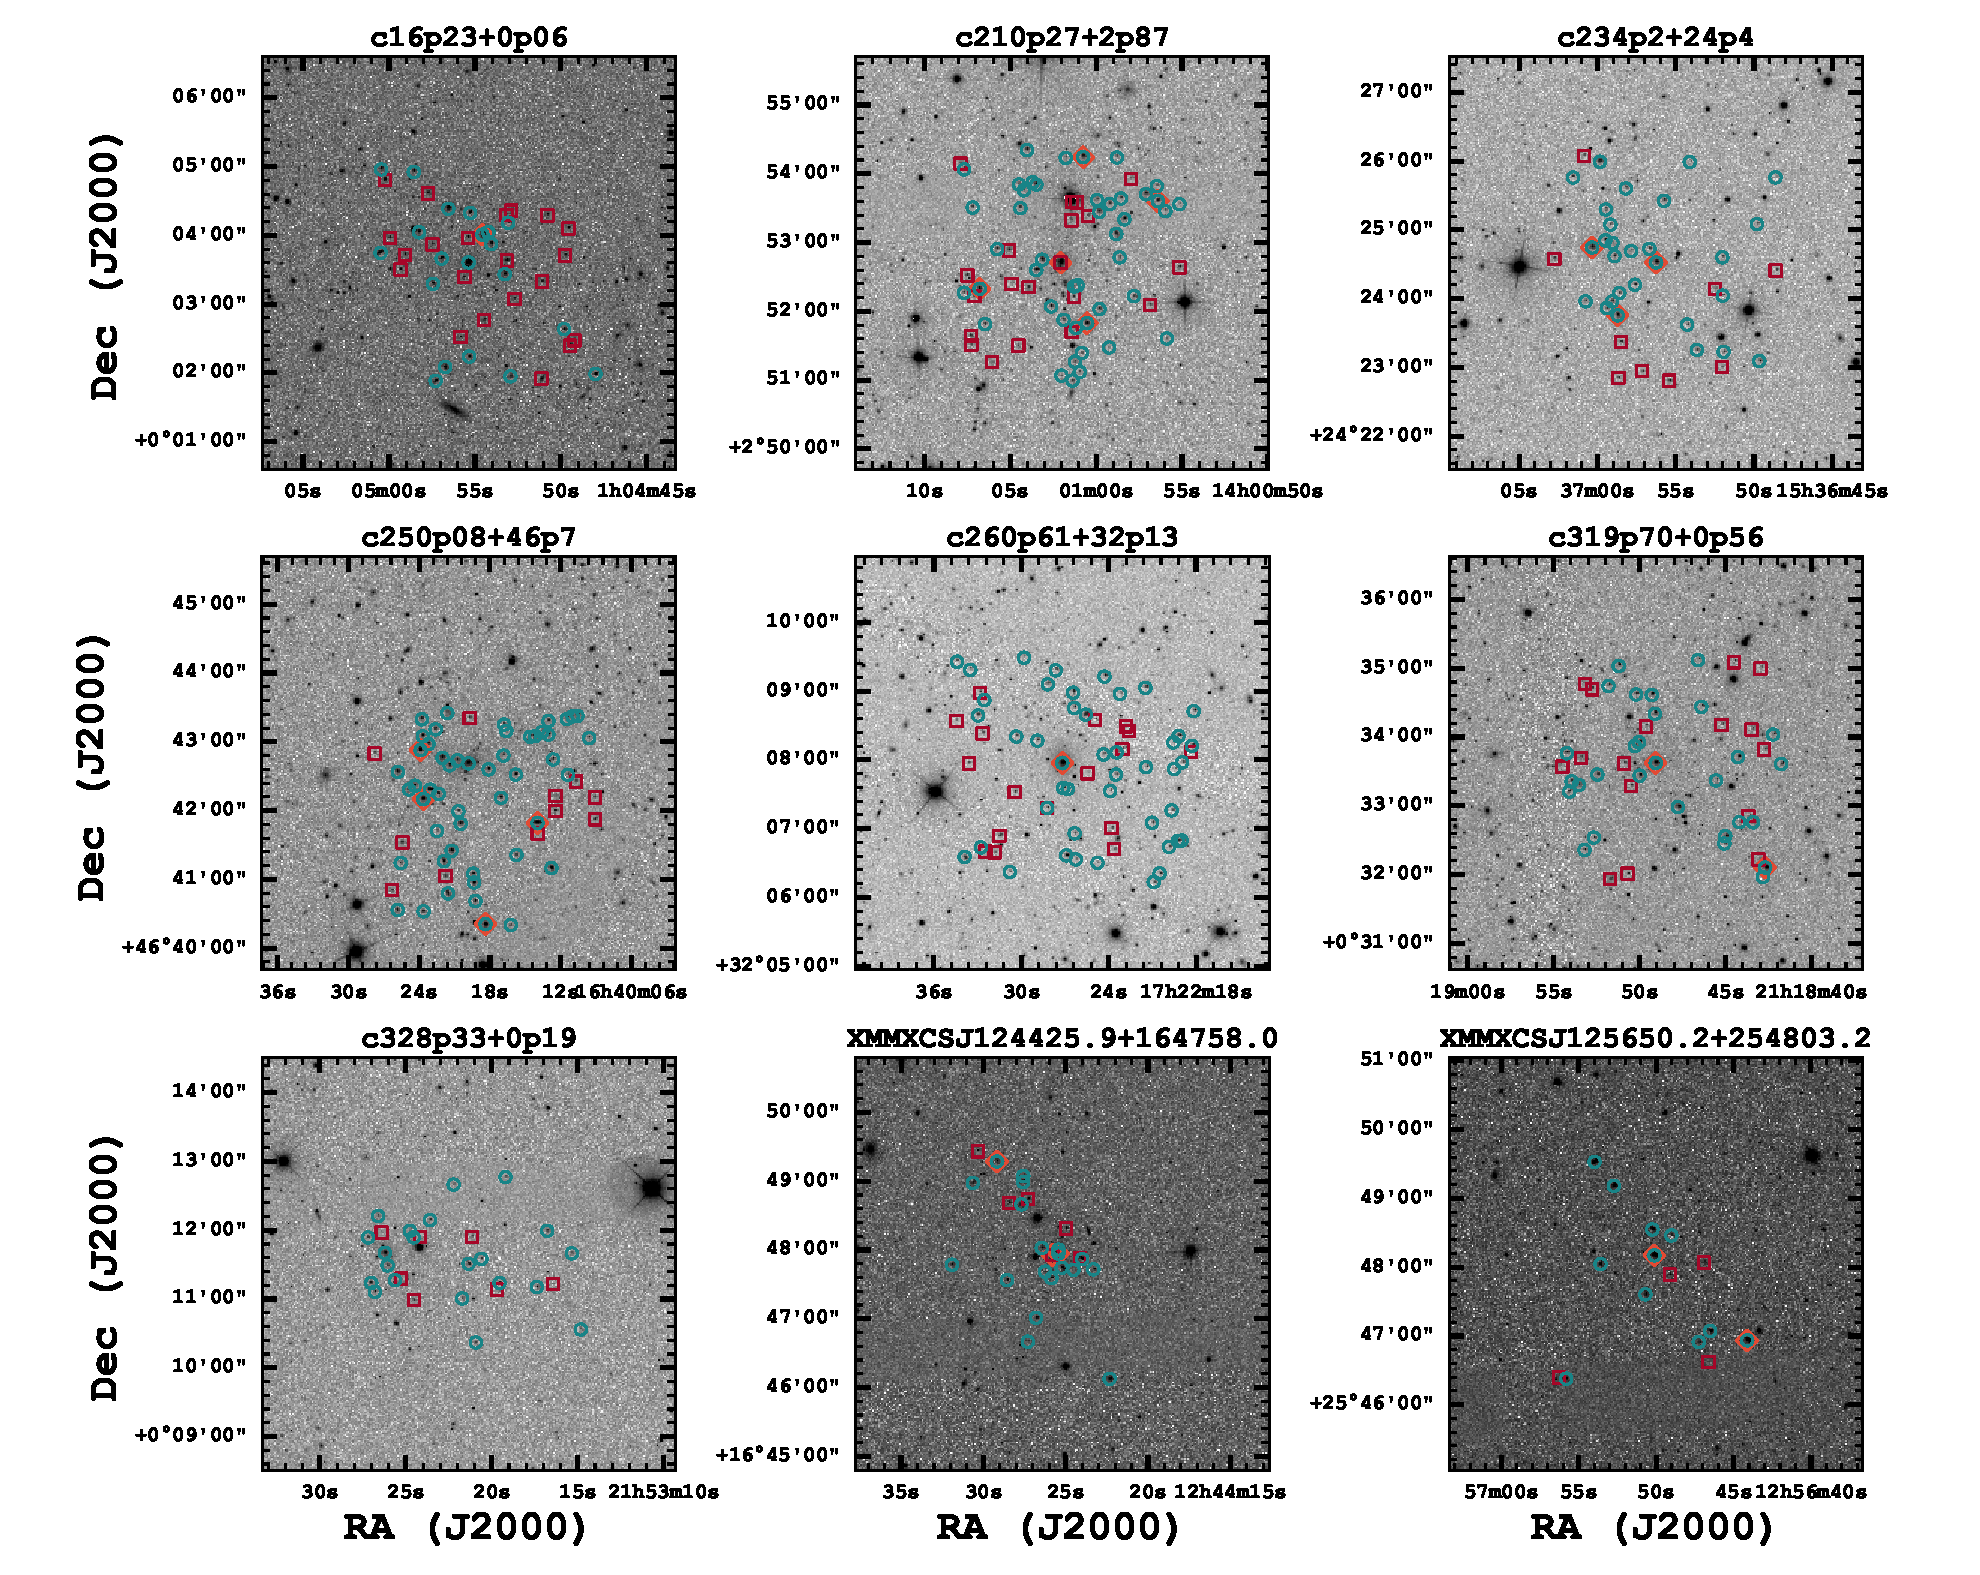
\includegraphics[width=\textwidth]{figures2/multimontage.pdf}
	\end{center}
	\caption[SDSS \sdssr-band images of the remaining nine clusters in our sample.]{SDSS \sdssr-band images of the remaining nine clusters in our sample. The symbols show the position of observed galaxies. Blue circles indicate galaxies with $Q=0$ or $Q=1$ spectroscopic redshifts, red squares indicate galaxies where a redshift could not be reliably determined, and the orange diamond corresponds to galaxies with pre-existing redshifts from the SDSS.}  
	\label{2fig:multimontage} 
\end{figure}

\subsection{Redshift Catalog}\label{2sec:redshift catalog} 
A redshift solution is determined for each galaxy by cross-correlating \citep{Tonry1979} each of the spectra with six galaxy template spectra from the SDSS\footnote{http://classic.sdss.org/dr7/algorithms/spectemplates/index.html} using a custom, Python-based interface\footnote{https://github.com/boada/redshiftCode} to the \textsc{xcsao} task in the \textsc{iraf} \textsc{rvsao} package \citep{Kurtz1992, Kurtz1998}. For each galaxy we select the spectral template with the highest cross-correlation coefficient and visually inspect the fit. During visual inspection a quality flag ($Q$) is assigned. High-confidence redshifts, clearly determined by at least two obvious features (such as the Ca$^+$ H, K and Ca G absorption features), receive $Q=0$. Spectra with only a single strong feature (\eg, \hbox{[\ion{O}{II}]} emission) are assigned $Q=1$. Redshifts resulting from dubious or no obvious features are assigned $Q=2$. Figure~\ref{2fig:MSJ133520.1+410004.1} shows representative example spectra for each of the $Q$ flags. For the determination of cluster properties we only consider galaxies with spectroscopic quality flags of $Q=0$ and $Q=1$. 

\begin{figure}[t]
	\begin{center}
		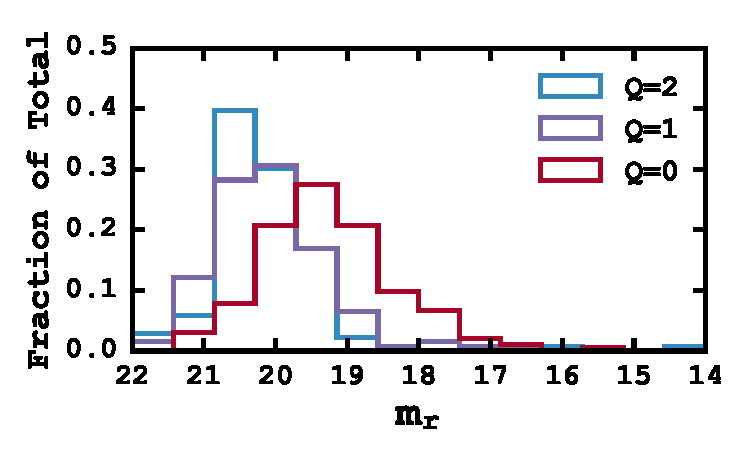
\includegraphics[width=\textwidth]{figures2/redshiftHist.pdf}
	\end{center}
	\caption[Redshift recovery fractions across all clusters.]{Redshift recovery fractions across all clusters. The bar heights represent the fraction of the total redshifts with the respective $Q$ value at a particular magnitude. For example, $\sim 40\%$ of the $Q=2$ redshifts have $m_r = 20.5-21$. We find a general decrease in redshift quality with increasing $m_r$. } 
	\label{2fig:redshiftHist} 
\end{figure}

Figure \ref{2fig:redshiftHist} shows the distribution of $Q$ values for the redshifts across all clusters. We attempt to estimate spectroscopic redshifts for 447 galaxies, of which 44\% have $Q=0$, 27\% have $Q=1$ and 29\% have $Q=2$.  We find a general decrease in $Q$ flag with increasing $m_r$. Approximately 30\% of the $Q=0$ redshifts correspond to galaxies with $19 < m_r <20$ mag whereas about 40\% $Q=2$ galaxies have $m_r = 20.5-21$ mag.

\pagebreak
While, \textsc{xcsao} reports errors on the cross-correlation redshift, previous work \citeeg{Quintana2000, Sifon2015a} shows the cross-correlation velocity uncertainties are underestimated by up to a factor of two. We report our redshift uncertainties as twice the uncertainty estimated by \textsc{xcsao}.

Redshift information, with $Q=0$ or $Q=1$ spectra, for each galaxy are given in Table~\ref{2tbl:MSJ133520.1+410004.1}. The right panel of Figure~\ref{2fig:MSJ133520.1+410004.1} shows selected spectra from cluster MSJ133520.1+410004.1 with corresponding best fitting SDSS template. See the appendix for the remaining nine clusters.

\begin{landscape}
	\singlespace
	\begin{longtable}{ccccccccccc} 
	\caption[Spectroscopic redshifts for galaxies in MSJ133520.1+410004.1 measured with the MS.]{Spectroscopic redshifts for galaxies in MSJ133520.1+410004.1 measured with the MS. Column 1: The telescope pointing; Column 2: The dither position; Column 3: The fiber number; Column 4: The right ascension of the galaxy; Column 5: The declination of the galaxy; Column 6: The the observed SDSS \sdssr\ magnitude; Column 7: The galaxy redshift; Column 8: The redshift $Q$ flag; Column 9: The galaxy membership information; Column 10: The clustercentric radial distance; Column 11: The LOSV of the galaxy with respect to the cluster. See the appendix for similar tables for the remaining nine clusters.}\\
	\hline
	tile & dither & fiber & RA (J2000) & DEC (J2000) & \sdssr\ (mag) & redshift & $Q$ & Member & R (Mpc) & LOSV (\kms) \\
	(1) & (2) & (3) & (4) & (5) & (6) & (7) & (8) & (9) & (10) & (11) \\
	\hline \hline
	\endfirsthead
	\multicolumn{4}{l}%
	{\tablename\ \thetable\ Continued} \\
	\hline
	tile & dither & fiber & RA (J2000) & DEC (J2000) & \sdssr\ (mag) & redshift & $Q$ & Member & R (Mpc) & LOSV (\kms) \\
	(1) & (2) & (3) & (4) & (5) & (6) & (7) & (8) & (9) & (10) & (11) \\
	\hline \hline
	\endhead
		NE & 1 & 14 & 13:35:27.004 & +41:01:36.20 & 20.47 & 0.2019$\pm{0.0003}$ & 1 & ... & 0.40 & -6945$\pm{146}$ \\
		NE & 1 & 111 & 13:35:24.177 & +41:00:54.16 & 20.10 & 0.1178$\pm{0.0001}$ & 1 & ... & 0.15 & -27397$\pm{63}$ \\
		NE & 1 & 154 & 13:35:23.853 & +41:00:33.19 & 19.28 & 0.2214$\pm{0.0002}$ & 0 & ... & 0.18 & -2214$\pm{83}$ \\
		NE & 2 & 6 & 13:35:21.777 & +41:01:34.15 & 20.38 & 0.1691$\pm{0.0002}$ & 1 & ... & 0.27 & -14929$\pm{102}$ \\
		NE & 2 & 14 & 13:35:26.632 & +41:01:33.06 & 20.95 & 0.0403$\pm{0.0003}$ & 0 & ... & 0.09 & -46214$\pm{131}$ \\
		NE & 2 & 63 & 13:35:20.998 & +41:01:08.49 & 17.90 & 0.2381$\pm{0.0001}$ & 0 & $\checkmark$ & 0.25 & 1849$\pm{49}$ \\
		NE & 3 & 22 & 13:35:22.879 & +41:01:24.60 & 19.76 & 0.2386$\pm{0.0003}$ & 0 & $\checkmark$ & 0.33 & 1961$\pm{131}$ \\
		NE & 3 & 25 & 13:35:24.669 & +41:01:26.21 & 19.54 & 0.1444$\pm{0.0001}$ & 0 & ... & 0.25 & -20924$\pm{58}$ \\
		NE & 3 & 73 & 13:35:18.447 & +41:01:00.60 & 19.63 & 0.0779$\pm{0.0001}$ & 0 & ... & 0.09 & -37080$\pm{29}$ \\
		NE & 3 & 106 & 13:35:20.957 & +41:00:50.19 & 18.83 & 0.2235$\pm{0.0002}$ & 0 & $\checkmark$ & 0.17 & -1691$\pm{78}$ \\
		NE & 3 & 147 & 13:35:19.341 & +41:00:31.82 & 19.48 & 0.2380$\pm{0.0001}$ & 0 & ... & 0.11 & 1822$\pm{73}$ \\
		NE & 3 & 185 & 13:35:24.990 & +41:00:18.06 & 20.51 & 0.1887$\pm{0.0002}$ & 1 & ... & 0.18 & -10169$\pm{83}$ \\
		NE & 3 & 206 & 13:35:20.095 & +41:00:04.12 & 16.39 & 0.2274$\pm{0.0001}$ & 1 & $\checkmark$ & 0.00 & -763$\pm{34}$ \\
		NE & 3 & 210 & 13:35:22.528 & +41:00:05.00 & 19.59 & 0.2242$\pm{0.0001}$ & 1 & $\checkmark$ & 0.10 & -1543$\pm{49}$ \\
		NW & 1 & 127 & 13:35:16.384 & +41:00:47.33 & 17.43 & 0.2377$\pm{0.0001}$ & 0 & $\checkmark$ & 0.23 & 1752$\pm{68}$ \\
		NW & 1 & 167 & 13:35:14.400 & +41:00:29.73 & 19.69 & 0.2333$\pm{0.0002}$ & 0 & $\checkmark$ & 0.26 & 690$\pm{117}$ \\
		NW & 2 & 27 & 13:35:17.216 & +41:01:27.25 & 20.21 & 0.1512$\pm{0.0002}$ & 0 & ... & 0.24 & -19279$\pm{117}$ \\
		NW & 2 & 63 & 13:35:12.486 & +41:01:10.57 & 18.84 & 0.1638$\pm{0.0001}$ & 0 & ... & 0.31 & -16210$\pm{44}$ \\
		NW & 2 & 73 & 13:35:09.729 & +41:01:03.49 & 20.00 & 0.2402$\pm{0.0001}$ & 1 & ... & 0.50 & 2367$\pm{58}$ \\
		NW & 2 & 165 & 13:35:12.728 & +41:00:25.16 & 18.74 & 0.2394$\pm{0.0001}$ & 0 & $\checkmark$ & 0.33 & 2155$\pm{58}$ \\
		NW & 2 & 171 & 13:35:16.434 & +41:00:25.31 & 21.68 & 0.1617$\pm{0.0002}$ & 1 & ... & 0.13 & -16728$\pm{121}$ \\
		NW & 2 & 173 & 13:35:17.911 & +41:00:27.16 & 19.49 & 0.1039$\pm{0.0002}$ & 0 & ... & 0.06 & -30763$\pm{107}$ \\
		NW & 2 & 220 & 13:35:10.891 & +41:00:03.07 & 19.45 & 0.2994$\pm{0.0002}$ & 0 & ... & 0.47 & 16739$\pm{102}$ \\
		NW & 2 & 239 & 13:35:13.582 & +40:59:54.58 & 20.24 & 0.2316$\pm{0.0002}$ & 1 & $\checkmark$ & 0.28 & 265$\pm{92}$ \\
		NW & 3 & 142 & 13:35:16.981 & +41:00:35.55 & 19.44 & 0.2233$\pm{0.0002}$ & 0 & $\checkmark$ & 0.17 & -1745$\pm{78}$ \\
		SE & 1 & 27 & 13:35:25.896 & +40:59:52.05 & 19.35 & 0.2295$\pm{0.0004}$ & 1 & $\checkmark$ & 0.25 & -238$\pm{170}$ \\
		SE & 1 & 46 & 13:35:19.779 & +40:59:41.85 & 18.73 & 0.2293$\pm{0.0002}$ & 0 & $\checkmark$ & 0.08 & -284$\pm{107}$ \\
		SE & 1 & 86 & 13:35:26.506 & +40:59:28.30 & 20.59 & 0.2255$\pm{0.0002}$ & 1 & $\checkmark$ & 0.29 & -1205$\pm{112}$ \\
		SE & 1 & 123 & 13:35:22.588 & +40:59:11.02 & 18.17 & 0.2307$\pm{0.0002}$ & 0 & $\checkmark$ & 0.22 & 44$\pm{102}$ \\
		SE & 1 & 129 & 13:35:26.254 & +40:59:08.50 & 19.42 & 0.1282$\pm{0.0002}$ & 0 & ... & 0.20 & -24863$\pm{107}$ \\
		SE & 2 & 164 & 13:35:20.600 & +40:58:48.65 & 20.02 & 0.2938$\pm{0.0001}$ & 0 & ... & 0.33 & 15369$\pm{53}$ \\
		SE & 3 & 157 & 13:35:25.857 & +40:58:53.46 & 18.31 & 0.1701$\pm{0.0001}$ & 0 & ... & 0.28 & -14684$\pm{29}$ \\
		SE & 3 & 171 & 13:35:25.332 & +40:58:48.88 & 19.49 & 0.2400$\pm{0.0003}$ & 0 & ... & 0.36 & 2296$\pm{126}$ \\
		SE & 3 & 198 & 13:35:24.191 & +40:58:35.23 & 20.83 & 0.1177$\pm{0.0002}$ & 1 & ... & 0.21 & -27419$\pm{87}$ \\
		SW & 1 & 41 & 13:35:17.295 & +40:59:47.40 & 19.87 & 0.2231$\pm{0.0002}$ & 0 & ... & 0.13 & -1808$\pm{107}$ \\
		SW & 1 & 114 & 13:35:17.529 & +40:59:15.55 & 20.60 & 0.2493$\pm{0.0003}$ & 1 & ... & 0.22 & 4561$\pm{156}$ \\
		SW & 1 & 224 & 13:35:13.709 & +40:58:25.25 & 20.03 & 0.1276$\pm{0.0003}$ & 0 & ... & 0.28 & -25006$\pm{126}$ \\
		SW & 1 & 227 & 13:35:15.509 & +40:58:27.26 & 19.27 & 0.2328$\pm{0.0002}$ & 0 & $\checkmark$ & 0.41 & 559$\pm{83}$ \\
		SW & 1 & 245 & 13:35:17.832 & +40:58:19.02 & 19.29 & 0.2211$\pm{0.0003}$ & 1 & ... & 0.39 & -2275$\pm{136}$ \\
		SW & 1 & 246 & 13:35:18.529 & +40:58:20.43 & 21.31 & 0.1970$\pm{0.0002}$ & 1 & ... & 0.34 & -8140$\pm{117}$ \\
		SW & 2 & 24 & 13:35:15.282 & +40:59:51.52 & 21.29 & 0.2225$\pm{0.0002}$ & 1 & $\checkmark$ & 0.20 & -1934$\pm{97}$ \\
		SW & 2 & 29 & 13:35:18.391 & +40:59:50.06 & 18.17 & 0.2405$\pm{0.0001}$ & 0 & ... & 0.09 & 2440$\pm{44}$ \\
		SW & 2 & 39 & 13:35:15.539 & +40:59:43.86 & 18.73 & 0.2263$\pm{0.0002}$ & 0 & $\checkmark$ & 0.20 & -1023$\pm{107}$ \\
		SW & 2 & 53 & 13:35:15.211 & +40:59:38.90 & 18.73 & 0.2412$\pm{0.0001}$ & 0 & $\checkmark$ & 0.23 & 2593$\pm{58}$ \\
		SW & 2 & 59 & 13:35:09.857 & +40:59:32.82 & 19.83 & 0.2334$\pm{0.0002}$ & 1 & $\checkmark$ & 0.45 & 697$\pm{107}$ \\
		SW & 2 & 65 & 13:35:13.725 & +40:59:31.94 & 20.58 & 0.3156$\pm{0.0003}$ & 0 & ... & 0.37 & 20688$\pm{156}$ \\
		SW & 2 & 86 & 13:35:17.737 & +40:59:25.25 & 19.71 & 0.2236$\pm{0.0002}$ & 0 & $\checkmark$ & 0.17 & -1684$\pm{78}$ \\
		SW & 2 & 90 & 13:35:11.098 & +40:59:19.79 & 20.41 & 0.2354$\pm{0.0002}$ & 0 & $\checkmark$ & 0.42 & 1195$\pm{97}$ \\
		SW & 3 & 26 & 13:35:16.763 & +40:59:48.52 & 17.94 & 0.2250$\pm{0.0001}$ & 0 & $\checkmark$ & 0.15 & -1334$\pm{34}$ \\
		SW & 3 & 37 & 13:35:14.503 & +40:59:43.50 & 19.79 & 0.2428$\pm{0.0002}$ & 0 & $\checkmark$ & 0.26 & 2979$\pm{107}$ \\
		SW & 3 & 65 & 13:35:13.944 & +40:59:28.57 & 18.60 & 0.2362$\pm{0.0001}$ & 0 & $\checkmark$ & 0.29 & 1385$\pm{58}$ \\
		SW & 3 & 73 & 13:35:10.002 & +40:59:23.42 & 19.52 & 0.2307$\pm{0.0001}$ & 0 & $\checkmark$ & 0.45 & 39$\pm{73}$ \\
	\hline 
	\label{2tbl:MSJ133520.1+410004.1} 
	\end{longtable}
\end{landscape}

\subsection{Cluster Membership}\label{2sec:cluster membership} 
We first determine the redshift of the cluster ($z_c$) as the average redshift of all cluster galaxies with Q=0 and Q=1. This serves as a zero-point from which all other galaxies will be compared. An incorrect cluster redshift introduces errors into the measured line of sight velocity (LOSV) and corresponding dispersion, which, in turn, contributes to errors associated with dynamical mass and radius. 

In simple terms, the cluster redshift is the mean of the redshifts of all galaxies associated with the cluster. However, because the standard mean can be quite sensitive to outliers or otherwise contaminated data, we use the biweight location estimator \citep{Beers1990} which provides improved performance. The biweight location provides protection against a small number of interlopers. Therefore, the process of determining $z_c$ and the cluster membership are linked. We begin with the nominal $z_c$ (see Table~\ref{2tbl:targets}) and apply an initial velocity cut of 5000 \kms\ to remove any foreground or background galaxies. Then, using the membership determination techniques described below we determine the member galaxies from which a new $z_c$ is calculated. The entire process is repeated until convergence, usually within a single iteration. The cluster central redshift and associated 68\% uncertainties, derived from bootstrap resampling, are given in Table~\ref{2tbl: derived parameters}.

To reject the galaxies not associated with the targeted cluster, we employ two methods depending on the number of galaxies associated with each cluster. For clusters with 20 or more $Q=0$ or $Q=1$ redshifts we use the ``shifting gapper'' method of \citeeg{Fadda1996, Crawford2014}, which combines both the positional and velocity information. Galaxies are first sorted by their radial separation from the cluster center (See Table~\ref{2tbl:targets}) and binned into radial bins of at least 10 members. Once in the radial bins, the galaxies are sorted by the LOSV, 
\begin{equation}
	LOSV = c\frac{(z-z_{c})}{(1+z_{c})} 
\end{equation}
where $c$ is the speed of light in \kms, $z$ is the redshift of the individual galaxy and $z_{c}$ is the redshift of the cluster. Any galaxy with a LOSV greater than 1000 \kms\ of a neighboring galaxy (the velocity ``gap'') is rejected as an interloper. The procedure repeats until the number of galaxies stabilizes in the bin. Once the members have been identified we recompute $z_c$, LOSVs, and begin the membership selection again. This entire process is repeated until the number of member galaxies remains constant. This is normally achieved within a single iteration. 

For galaxy clusters with fewer than 20 $Q=0$ or $Q=1$ redshifts we employ the general of membership determination method outlined in \cite{Wilman2005, Connelly2012}. We assume an initial velocity dispersion, $\sigma(v)$, of 500$(1+z)$ \kms\ and apply both redshift and spatial limits given by: 
\begin{equation}
	\delta(z)_{max} = 2 \sigma(v)/c 
\end{equation}
and 
\begin{equation}
	\delta(r)_{max} = \frac{c\times\delta(z)_{max}}{bH(z)} 
\end{equation}
where $b=9.5$ is the aspect ratio between the projected spatial and line-of-sight dimensions, $H(z) = H_0 E(z)$ and $E(z) = \sqrt{\Omega_m(1+z^3)+\Omega_{\Lambda}}$. We select all galaxies with $|z-z_c| < \delta(z)_{max}$ and radial separation, $R$, $<\delta(r)_{max}$. During each step, we update both the $z_c$ and $\sigma(v)$ using the identified members and this process is repeated until the number of member galaxies converges, usually within three iterations.

To calculate the velocity dispersion in this membership determination method, we use the gapper estimator \citep{Beers1990} which provides accurate dispersions for groups as small as five members \citep{Hou2009}. It is given by 
\begin{equation}
	\sigma_g = \frac{\sqrt{\pi}}{N(N-1)} \sum_{i=1}^{N-1} w_i g_i
\end{equation}
where $N$ is the number galaxies, the weights are $w_i = i(N-i)$ and $g_i = LOSV_{i+1} - LOSV_i$ are the gaps between ordered pairs of radial LOSVs. The dispersion estimate is corrected by $1.135$ to account for the $2\sigma$ redshift space cut applied during membership determination \citep{Connelly2012}. We follow this method for the calculation of the dispersion for consistency in member determination only. The final velocity dispersion of each cluster is determined in the following subsection.

Membership information for cluster MSJ133520.1+410004.1 is given in Column 9 of Table~\ref{2tbl:MSJ133520.1+410004.1}. See the appendix for the membership of the other observed clusters.

\subsection{Line-of-Sight Velocity Dispersion}\label{2sec:LOSVD}
To compute the line-of-sight velocity dispersion (LOSVD) of each cluster we follow the maximum likelihood method of \cite{Walker2006}. We assume that the each galaxy is drawn from a Gaussian distribution centered on the mean cluster velocity and we maximize the log of the product of each cluster member's individual Gaussian probabilities (their Eq. 8):
\begin{equation}
  \label{2eq:log}
\ln(p)=-\frac{1}{2}\sum_{i=1}^{N}\ln(\sigma_i^2+\sigma_p^2)-\frac{1}{2}\sum_{i=1}^N\frac{(v_i-\langle u \rangle)^2}{(\sigma_i^2+\sigma_p^2)}-\frac{N}{2}\ln(2\pi).
\end{equation}
where $N$ is the number of member galaxies, $\sigma_p$, $\langle\mu\rangle$, and $\sigma_i$ are the LOSVD, the average radial velocity and the error on the individual LOSVs respectively. To maximize the probability, we use {\sc emcee}\footnote{http://dan.iel.fm/emcee/current/} \citep{Foreman-Mackey2013}, a Monte Carlo Markov Chain (MCMC) sampler, based on affine-invariant ensemble sampler (see \citealt{Goodman2010} for details on affine-invariant samplers). We set priors on $\langle\mu\rangle$, and $\sigma_p$ by requiring that $\langle\mu\rangle$ lies between the maximum and minimum LOSV and that $\sigma_p$ be positive and less than $1400$ \kms which corresponds approximately to a $10^{16}$ \Msol\ cluster at $z=0$, larger than any expected cluster mass in our sample. We draw twenty thousand samples from the posterior probability distribution and report a measured LOSVD as the median value of the posterior probability distribution with 68\% error bars defined as the square root of the second moment of the same distribution.

\section{Estimating Cluster Masses}
The goal of this section is to describe the methods used to estimate (or predict) the total masses of the clusters in our sample. We test two distinct approaches. We begin the discussion with a traditional power law (PL) based approach where we estimate the cluster mass based on the LOSVD measurement. The second is a machine learning (ML) based approach where we use a combination of cluster observables to predict a cluster mass. The ML approach requires additional discussion about the creation of a suitable training set. We conclude with an examination of how this training set can potentially influence the results of the ML method.   

\subsection{PL Estimates of Cluster Mass}
We adopt the scaling relation of \cite{Munari2013} to estimate cluster masses based solely on their LOSVD. The scaling relation is based on the work of \cite{Evrard2008} and has the form: 
\begin{equation}\label{2eq:power law}
	M_{200c} = \frac{10^{15}}{h(z)} \bigg{(}\frac{\sigma_{1D}}{A_{1D}} \bigg{)}^{1/\alpha} \Msol 
\end{equation}
where $A_{1D} =1177\pm4.2$ \kms, $\alpha = 0.364\pm0.0021$, $h(z) = H(z)/100$, and $\sigma_{1D}$ is the LOSVD. The relation is calibrated through a cosmological simulation using galaxies (instead of dark matter particles or subhalos) as the tracers of LOSVD. This choice of tracer results in dynamical masses which are $16-26\%$ lower \citeeg{Kirk2015, Sifon2015a} than masses obtained through the scaling relation of \cite{Evrard2008}, which has been calibrated using dark matter particles alone. This is due to dynamical effects which act upon the galaxies but not the dark matter particles.

We use the cluster redshift, given in Column 5, and the LOSVD values given in Column 6 of Table~\ref{2tbl: derived parameters} along with Equation~\ref{2eq:power law} to estimate the total mass of our ten clusters. The log of the predicted mass for each cluster is given in Column 7 of Table~\ref{2tbl: derived parameters}.

\subsection{Supervised Machine Learning}\label{2sec:ML methods}
Supervised ML provides an algorithm to infer the relationship between a set of known input variables (features) and a set of desired outputs (targets), through the use of a training set (see Section 2). The training set consists of both features and desired targets, which the ML algorithm uses to ``learn'' their relationship. The algorithm is then provided with a dataset consisting of only the features, and uses the inferred relationship to predict appropriate target values. Part of the training set is often reserved as a \emph{testing} set \citeeg{Ripley2007, Xu2013, Ntampaka2015, Ntampaka2015a, Acquaviva2016} which is used to both select and train the specific ML algorithm.

Just as in Section 2, we rely on an ensemble ML method \citeeg{Caruana2006} known as a forest of randomized decision trees (or random forest; RF; \citealt{Ho1995, Ho1998}), which we prefer due to their straightforward design and easily accessible uncertainty estimates. A RF is a type of ensemble method where the trees can be visualized as flow chart. The path through the flow chart (the trees) is decided by the values of the training features at each fork. RF use a random subset of the train data to decide which fork should be followed. The final prediction is the mean of each tree's final value. We optimize the input parameters (often called hyper-parameters) of our RF by further splitting our testing set into a cross-validation (CV) set. We use 5-fold CV, where the testing set is split (folded) five times, throughout. The RF methods implemented in this work are part of the {\sc Scikit-Learn} \citep{Pedregosa2012} Python library.

Building off the work in Section 2, we use the ``Buzzard'' semi-analytical model to provide both the observable features and desired targets in order to train our ML method. The Buzzard mock galaxy catalog contains 238 million galaxies with \sdssr\ mag $< 29$ and $z \leq 8.7$. The galaxies are located in a 398.49 \degsq\ portion of the sky and their luminosities are derived from a combination of Sub-halo Abundance Matching (SHAM; \citealt{Reddick2013}) and Adding Density Dependent Spectral Energy Distributions (ADDSED). The galaxies are assigned to the dark matter halos identified by the {\sc ROCKSTAR} halo finder \citep{Behroozi2013}. The catalogs assume the following cosmological parameters: $\Omega_\Lambda = 0.714$, $\Omega_M = 0.286$, $\sigma_8 = 0.82$ and $H_0= 70$ \kms \mpc, which we have also adopted for general use in this work. See Section 2 for a more thorough description of the process used to create the catalogs.

\subsection{ML Based Observations}
In order to create a mock dataset which resembles our actual observations we first rely on the RF method as a classifier. The goal is to assign each galaxy in the Buzzard catalog a $Q$ flag of either 0, 1 or 2 based on their observed magitudes in the five SDSS filters, \sdssu\sdssg\sdssr\sdssi\sdssz, the ten combinations of possible colors, and the square of those colors. \cite{Acquaviva2016} uses a similar feature set to predict the metallicity of SDSS galaxies with good effect. 

The classifier is trained using the redshift catalog derived from our cluster observations (Section \ref{2sec:redshift catalog}), and the 447 observations are split into a training, CV and test sample. We use the training set to train the ML method, the CV set to tune the model hyper-parameters and the test sample to verify how well our model classifies each galaxy. We also perform recursive feature elimination to remove features which contribute very little to the classification.

We compute two statistics to evaluate how well our model classifies the galaxies, the recall and the precision. The recall is the number predicted compared to the true number of classifications, $N_{pred}/N_{true}$. The precision is the number of correct predictions compared to the total number of predictions for each class, $N_{corr}/N_{pred}$. In both cases the metrics range from zero to one, and higher numbers are better. For our optimized RF classifier we achieve overall recall and precision of $\sim60\%$. For the individual classes ($Q$ flags), the RF classifier performs significantly better when classifying $Q=0$ and $Q=2$ galaxies, with recall rates well above 70\%. The $Q=1$ training galaxies have significant overlap between $Q=0$ and $Q=2$ (see Figure \ref{2fig:redshiftHist}) which leads to a recall for $Q=1$ galaxies of only $\sim20\%$. 

Figure~\ref{2fig:redshiftHist} shows there is significant overlap between the $Q$ flags. In our testing, we find no combination of features which wholly separates the $Q$ flags, providing a high level of confusion for the RF. We find similar levels of recall and precision for other ML classification methods besides RF.

\begin{figure}[t]
	\begin{center}
		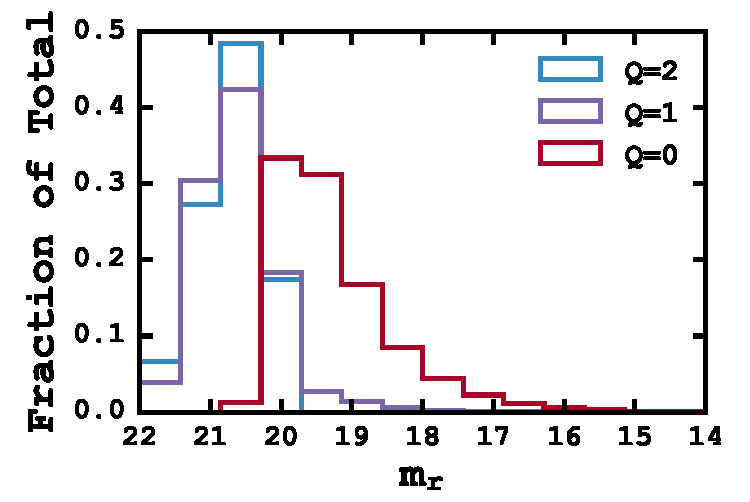
\includegraphics[width=\textwidth]{figures2/buzzardQHist.pdf}
	\end{center}
	\caption[Quality flag assignments for the 2.7 million Buzzard catalog galaxies with $\sdssg< 22$ mag.]{Quality flag ($Q$) assignments for the 2.7 million Buzzard catalog galaxies with $\sdssg< 22$ mag. The bar heights represent the fraction of the total redshifts with the respective $Q$ value at a particular magnitude. The distributions resemble the actual observations in Figure \ref{2fig:redshiftHist}. See the text for a detailed explanation of the classification process.} 
	\label{2fig:buzzardHist} 
\end{figure}

We assign each galaxy in the Buzzard catalog with $z<0.5$ and $\sdssg< 22$ mag a $Q$ flag using the optimized RF classifier trained with all 447 observations. Figure \ref{2fig:buzzardHist} shows the $Q$ flag distribution as a function of \sdssr\ magnitude. The total distribution of the 2.7 million $Q$ flags is 45.6\% $Q=0$, 24.7\% $Q=1$, and 29.6\% $Q=2$. This distribution closely resembles the fractions of the actual observations with some $Q=1$ galaxies misclassified as $Q=0$. Because we use galaxies with either $Q=0$ or $Q=1$ this is does not significantly bias our analysis.

\subsection{ML Based Cluster Masses}\label{2sec:ML based cluster masses}
We use the galaxies with reliably measured spectroscopic redshifts ($Q=0$ and $Q=1$) created in the previous subsection to construct total mass distributions of the mock clusters. For this task we again use a RF, not as a classifier but as a regressor, which predicts a cluster mass given a set of input features, such as the observed LOSVD and redshift. Similarly to our classification methods, we create an optimized ML method by splitting the Buzzard catalogs into a training, CV, and testing set. 

Because the cluster masses presented with this method are predictions based on the feature data, any uncertainties quoted by this method are prediction intervals not confidence intervals. Prediction intervals are an estimate of the interval encompassing future observations, with a given probability. Confidence intervals, on the other hand, describe the different moments of a population. The prediction intervals are unique to each prediction, and are often based on the underlying assumption of normally distributed residuals. RF estimators do not assume normally distributed residuals, and thus, require special treatment.  

The prediction intervals for our RF estimator as based on the method of quantile regression forests \citep{Meinshausen2006}. The basic principle is that we record all response variables (the predictions), not simply the mean. This allows us to give the prediction as the full conditional probability distribution of all possible predictions. For brevity, we quote predicted masses as the median prediction and the 68\% prediction interval as the square root of the second moment of the full conditional probability distribution.

\subsection{The Importance of Training Features}\label{2sec: training features}
\begin{figure}[!ht]
	\begin{center}
		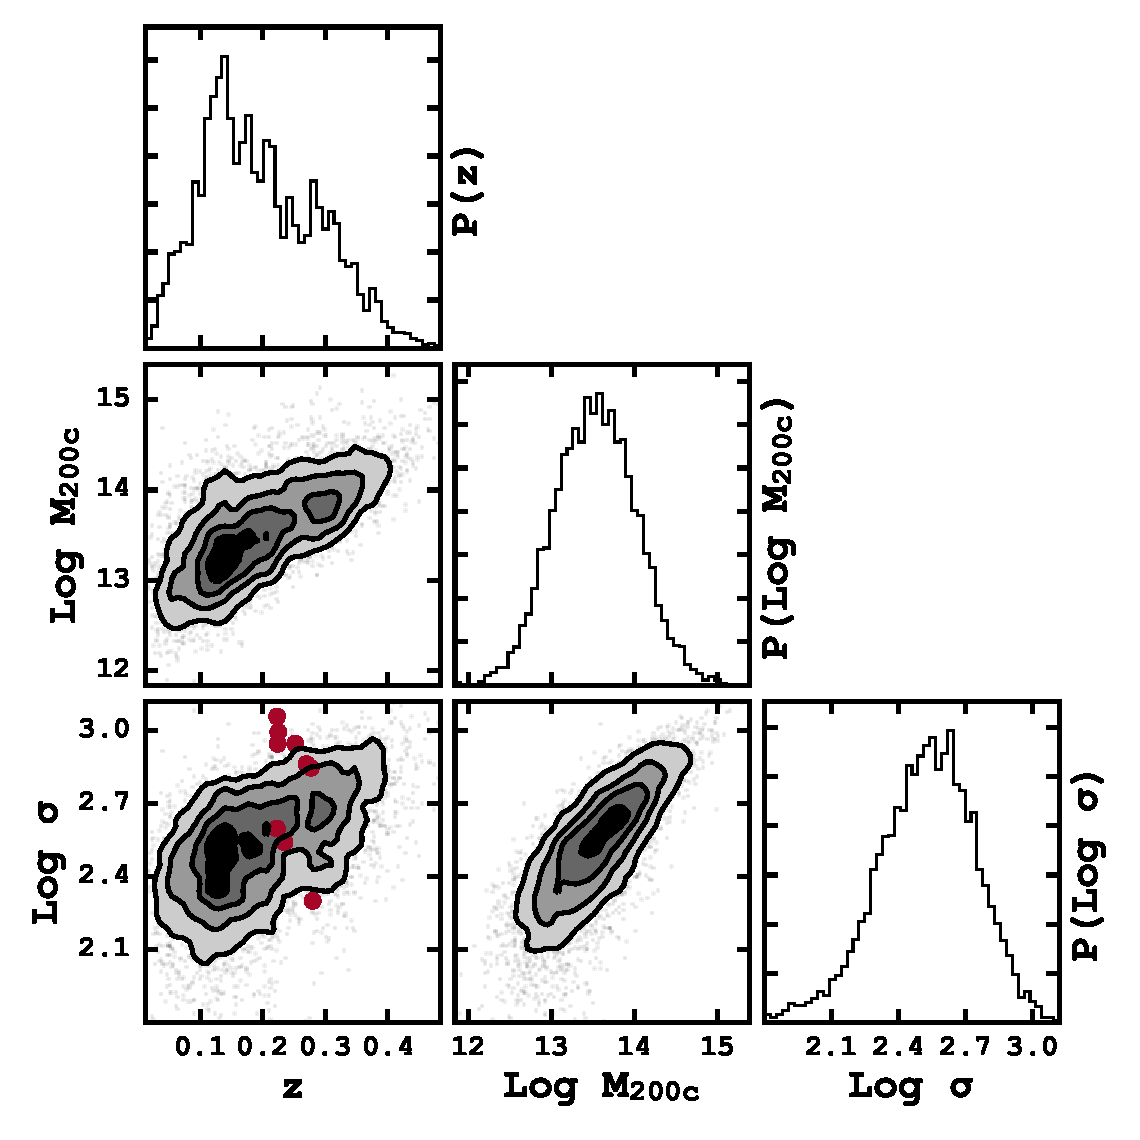
\includegraphics[width=\textwidth]{figures2/buzzardCorner.pdf}
	\end{center}
	\caption[Contour plot of the \emph{training} data with features $\sigma$ and $z$.]{Contour plot of the \emph{training} data with features $\sigma$ and $z$. The corner plots shows all of the one and two dimensional posterior probability distributions used to determine the correct cluster mass. The colored circles show the position in the log $\sigma$-redshift plane of the ten clusters in this sample.}
	\label{2fig:buzzardCorner}
\end{figure}

The data used to train our ML algorithm is critical to the success of the method. We require training data which is broad enough to expose the ML method to a wide enough range of cluster parameters as not to influence the final outcome. The features of our training sample can be selected such that it does not bias the final predictions in an expected way. Figure~\ref{2fig:buzzardCorner} shows the $\sigma$ and $z$ features of the training sample from the Buzzard catalogs.\footnote{Contour plots based on \cite{Foreman-Mackey2016}.} The large red circles indicate the observed positions of our ten clusters in relation to the training data. Immediately noticeable, is that our observed clusters occupy a narrow redshift range ($0.2< z <0.3$). We also notice that seven of the ten clusters sit at the top edge of the training data in the $z$-log $\sigma$ plane. Because the observed clusters are separate from the training data, the accuracy of the predictions of the cluster masses will be diminished. Below, we consider alternative training datasets which give improved cluster mass predictions when compared to the PL cluster mass estimates.

Because the of the difference in cosmological volume covered by the SDSS and simulated by Buzzard, there are too few clusters in Buzzard, at $z\sim0.2$, and with $\sigma$ as large as the clusters in our sample. Predictions based on the Buzzard catalogs give a higher likelihood that clusters at $z\sim0.2$ will be of lower total mass, when the redshift is included as a feature. This becomes apparent by examining the $z$-log $M_{200c}$ plane in Figure~\ref{2fig:buzzardCorner}. The vast majority of clusters with $0.2< z <0.3$ have masses between $10^{13} - 10^{14}$ \Msol, whereas the observed LOSVD ($\sigma$) values of our clusters would place them above $10^{15}$ \Msol. 

To combat the effect of cluster mass under-prediction, we make two critical changes from our method presented in Section 2. First, instead of using the membership information provided by the Buzzard catalogs we observe the clusters much in the same way we have with our actual observations. We select all galaxies within $2\farcm3$ around the center of each cluster (see Figure~\ref{2fig:tiles} for an illustration), and determine the cluster membership using the methods described in Section~\ref{2sec:cluster membership}. This serves to broaden the LOSVD distribution of the training data as both true member galaxies will be excluded and interloping galaxies will be erroneously included. Second, we exclude the redshift information from the training features when predicting the cluster masses. This has the effect of flattening the halo mass function (HMF), allowing for high mass clusters to exist at all redshifts. However, the fewer training features also lowers the predictive power through an increase in both the bias and scatter (see Figure~\ref{fig: ML comparison} as an example). 

Furthermore, we create an additional training dataset with a truly flat HMF. We flatten the HMF by selecting clusters in a range of true mass bins with uniform probability. In true cluster mass bins where there are too few clusters to randomly select the desired number of samples, we generate ``new'' clusters by rotating the viewing angle of each cluster and then re-observing the cluster in the new orientation. This creates a uniform true cluster mass distribution from which we train the ML algorithm. 

\section{Results and Discussion}\label{2sec:results}
The goal of this work to perform a practical test of some of the potential applications of a HETDEX-like survey to cluster science. Here, we present the predicted total masses of our ten clusters and estimate the absolute scale and scatter of a richness-mass relation based on those cluster masses. Because the accuracy of the predicted cluster masses is paramount to a well constrained richness-mass relation, we combine our results presentation with a discussion on their accuracy. 
 
\subsection{Cluster Masses}
\begin{figure}[!ht] 
	\begin{center}
		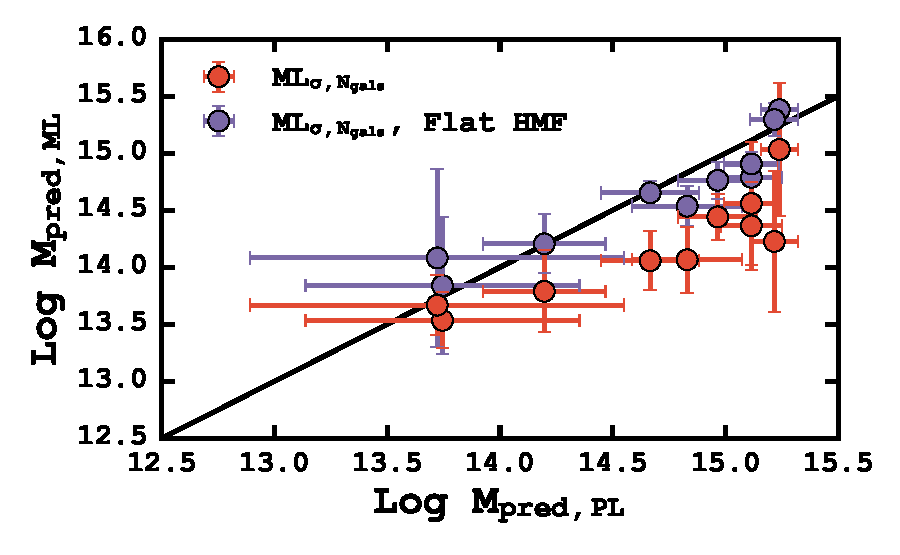
\includegraphics[width=\textwidth]{figures2/massCompare.pdf} 
	\end{center}
	\caption[Comparison of the cluster mass estimates for the PL scaling relation and the ML based mass predictions for the ten clusters in our observed sample.]{Comparison of the cluster mass estimates for the PL scaling relation (Equation~\ref{eq:power law}) and the ML based mass predictions for the ten clusters in our observed sample. The orange points show the $\mathrm{ML}_{\sigma, N_{gal}}$ predicted cluster masses using the Buzzard catalogs as a training set. The purple points represent $\mathrm{ML}_{\sigma, N_{gal}}$ predictions based on a flattened Buzzard HMF which leads to an improved performance when compared to the PL cluster mass estimates. The solid black line shows the 1:1 relation. See text for a description of the process used to create the three estimates of cluster mass.}
 \label{2fig: ML comparison} 
\end{figure}

In Section 2, we find the ML based method with the LOSVD ($\sigma$), redshift ($z$) and number of galaxies observed ($N_{gal}$) showed both the smallest bias and scatter over the largest range of cluster masses. This worked well because the training data were selected from a volume of similar size to the survey in question. As discussed previously, we modify our analysis slightly and use the PL based approach (Eqn.~\ref{2eq:power law}) and the $\mathrm{ML}_{\sigma, N_{gal}}$ method to estimate the masses of our ten clusters. This change in the ML method is the result of the differences in the cosmological volume of the SDSS and the Buzzard at $z\sim0.2$.  

The PL predicted masses versus the ML predicted masses are shown in Figure~\ref{2fig: ML comparison}. The orange points show our $\mathrm{ML}_{\sigma, N_{gal}}$ predicted masses using the cluster abundances as given in the Buzzard catalog. The purple points are the $\mathrm{ML}_{\sigma, N_{gal}}$ estimates when the Buzzard catalog HMF has been flattened. 

\pagebreak
The uniform true cluster mass distribution decreases the frequency that clusters of lower mass dominate (by number) at any individual velocity dispersion which reduces the likelihood the ML will underestimate the predicted cluster mass due to the underlying distribution of training clusters. If there are many more low and intermediate mass clusters compared to high mass clusters, as is the case in the Buzzard catalogs, the ML algorithm is more likely to predict a low or intermediate cluster mass as those objects are much more frequent in the training sample. Because of this change, the $\mathrm{ML}_{\sigma, N_{gal}}$ trained on a flatten HMF predicts cluster masses similar to those of the PL. However, the flattening of the HMF increases the scatter at fixed true cluster mass for training features. This leads to little or no reduction in the amount of scatter in the predicted cluster masses for a fixed true cluster mass when compared to the scatter in the PL estimates of cluster mass.

Therefore, we elect to use the PL estimated cluster masses for as the primary cluster mass estimates for the remainder of this study. The $\mathrm{ML}_{\sigma, N_{gal}}$ with a default HMF cannot reliably predict cluster masses for the highest mass clusters, and flattening the HMF, while improving the cluster mass predictions when compared to the PL estimates, does not accurately represent the universe. This underscores the need for a set of training data which accurately represents the cosmological volume being studied.

Furthermore, in Section 2, the cluster mass prediction process uses two steps. Firstly the cluster mass is predicted, and then the cluster mass is corrected by considering the bias and scatter of the training data. Here, we choose not to correct the cluster masses predicted by either the PL or ML method due to the dissimilarity between the training data and our observations. During our testing, we find that there are too few training clusters with masses $> 10^{15}$ \Msol, using an unmodified HMF, to place reliable contraints on the bias and scatter. As we discuss below, these high mass cluster constitute the bulk of our sample. Because we are unable to provide these clusters, with bias corrections, we choose to not correct any cluster mass estimate, to facilitate consistency throughout. 

The lack of a bias correction does not strongly effect our analysis as we are primarily interested in the scatter of our cluster masses. The scatter is unaffected as the individual mass estimates are scaled up or down by a common factor.

Table~\ref{2tbl: derived parameters} presents a summary of the derived parameters for each cluster. We include the LOSVD, the estimated cluster redshift, and the number of member galaxies observed. We provide two predicted cluster masses, the PL based cluster mass and the $ML_{\sigma, N_{gal}}$ predicted cluster mass. We discuss the accuracy of both of these predictions in the following subsections.

\begin{landscape}
	\begin{table}
	\caption[Summary of derived cluster parameters.]{Summary of derived cluster parameters: Column 1: The cluster name; Column 2: The number of SDSS sources observed; Column 3: The number of $Q=0(1)$ sources; Column 4: The number of member galaxies; Column 5: The redshift of the cluster; Columns 6: The LOSVD; Column 7: The PL predicted cluster mass; Column 8: The ML predicted cluster mass.} 
	\begin{tabular}{lccccccc} 
		\hline 
		&&&&&& PL & ML \\
		Cluster & Sources & Q=0 (1) & Member & $z_{c}$ & $\sigma$ (\kms) & log $M_{pred}$ & log $M_{pred}$ \\
		(1) & (2) & (3) & (4) & (5) & (6) & (7) & (8) \\
		\hline \hline 
		MSJ010455.4+000336.3 & 41 & 10 (10) & 15 & 0.2727$\pm{0.0029}$ & 1194$\pm{135}$ & 15.11$\pm{0.14}$ & 14.84$\pm{0.18}$ \\
		MSJ133520.1+410004.1 & 67 & 35 (17) & 25 & 0.2310$\pm{0.0025}$ & 1314$\pm{91}$ & 15.24$\pm{0.08}$ & 14.71$\pm{0.47}$ \\
		MSJ140102.0+025242.6 & 67 & 14 (30) & 16 & 0.2543$\pm{0.0035}$ & 1295$\pm{115}$ & 15.22$\pm{0.11}$ & 14.55$\pm{0.45}$ \\
		MSJ153656.3+242431.6 & 37 & 14 (14) & 11 & 0.2255$\pm{0.0034}$ & 932$\pm{189}$ & 14.83$\pm{0.24}$ & 14.21$\pm{0.16}$ \\
		MSJ164019.8+464241.5 & 61 & 36 (14) & 32 & 0.2274$\pm{0.0020}$ & 1183$\pm{121}$ & 15.11$\pm{0.12}$ & 14.96$\pm{0.23}$ \\
		MSJ172227.2+320757.2 & 61 & 26 (18) & 23 & 0.2260$\pm{0.0022}$ & 1044$\pm{154}$ & 14.97$\pm{0.18}$ & 14.54$\pm{0.14}$ \\
		MSJ211849.1+003337.3 & 45 & 21 (8) & 18 & 0.2750$\pm{0.0026}$ & 820$\pm{148}$ & 14.67$\pm{0.22}$ & 14.30$\pm{0.12}$ \\
		MSJ215422.9+003723.5 & 28 & 19 (2) & 16 & 0.2167$\pm{0.0026}$ & 547$\pm{124}$ & 14.20$\pm{0.27}$ & 14.04$\pm{0.09}$ \\
		XMMXCSJ124425.9+164758.0 & 25 & 11 (8) & 6 & 0.2316$\pm{0.0033}$ & 375$\pm{191}$ & 13.75$\pm{0.61}$ & 13.60$\pm{0.14}$ \\
		XMMXCSJ125650.2+254803.2 & 15 & 8 (3) & 3 & 0.2821$\pm{0.0059}$ & 372$\pm{258}$ & 13.72$\pm{0.83}$ & 13.52$\pm{0.13}$ \\
		\hline 
		\end{tabular}
		\label{2tbl: derived parameters} 
	\end{table}
\end{landscape}

\subsection{Notes for Individual Clusters}
Here we compare our PL inferred masses for the clusters in our sample to the previously reported estimates from the literature. \cite{Sifon2015} report total cluster masses for four of our clusters based on LOSVD measured from targeted spectra obtained with the Canada-France-Hawaii Telescope. They convert the LOSVD into a dynamical cluster mass using the PL scaling relation of \cite{Evrard2008} (which is the basis of our Equation~\ref{2eq:power law}) and estimate the uncertainties using jackknife resampling. One of our clusters has a reported LOSVD measurement and two have X-ray temperature measurements. On the whole, our PL estimated cluster masses are consistent with those previously reported in the literature; this stresses the utility of measuring cluster masses with IFU spectroscopy. In the following section we will discuss the ML estimated masses.

\subsubsection{MSJ133520.1+410004.1 (Abell 1763)}
\cite{Sifon2015} observe 103 member galaxies within $r_{200}$. They compute a LOSVD of 1130$\pm81$ \kms, compared to our 1314$\pm91$ \kms\ based on 25 member galaxies. They report a $M_{200c} = (14.6\pm3.1) \times 10^{14}$ \Msol, compared to our value of $M_{200c} = (17.4\pm3.2) \times 10^{14}$ \Msol. The two estimates are consistent within the given errors, and the difference is due to our higher measured LOSVD.

\subsubsection{MSJ140102.0+025242.6 (Abell 1835)}
\cite{Sifon2015} report a $M_{200c} = (4.5\pm1.9) \times 10^{14}$ \Msol, based on 41 member galaxies within
$r_{200c}$. We estimate a significantly different mass of $M_{200c} = (16.6\pm4.2)\times 10^{14}$ \Msol.
This discrepancy is due to the large difference in measured LOSVD, 762$\pm106$ \kms\ versus our
1295$\pm115$ \kms. However, \cite{Hoekstra2012} report a LOSVD for MSJ140102.0+025242.6 of 1218 \kms.
\cite{Geller2013} find $M_{200c} = (16.57\pm1.86)\times 10^{14}$ \Msol\ from the best fitting caustic mass
profiles, which is similar to our reported value. Using \emph{Chandra} X-ray observations,
\cite{Bonamente2012} report a $M_{200c} = (8.35$\err{0.86}{0.81}$)\times 10^{14}$ \Msol. While our cluster
mass estimate is not consistent with \cite{Sifon2015}, we find it is very similar to other reported mass
estimates based on virial techniques.

\subsubsection{MSJ164019.8+464241.5 (Abell 2219)}
With the largest number of member galaxies observed (of our sample), \cite{Sifon2015} use 241 member galaxies within $r_{200c}$ to estimate a mass of $M_{200c} = (17.0\pm2.8)\times 10^{14}$ \Msol. We estimate $M_{200c} = (12.9\pm3.6)\times 10^{14}$ \Msol. Using weak lensing techniques, \cite{Applegate2014} report a mass of $(12.0$\err{1.5}{1.5}$)\times 10^{14}$ \Msol\ within 1.5 Mpc, similar to our reported mass estimate.

\subsubsection{MSJ172227.2+320757.2 (Abell 2261)}
For MSJ172227.2+320757.2 we estimate $M_{200c} = (9.3\pm3.9)\times 10^{14}$ \Msol\ compared to $M_{200c} = (7.0\pm2.0)\times 10^{14}$ \Msol from \cite{Sifon2015}. They base their estimate on 76 member galaxies within $r_{200c}$. There is reasonable agreement between the two estimates.

\subsubsection{MSJ215422.9+003723.5 (Abell 2392)}\label{2sec: Abell2392}
The predicted mass of this cluster is significantly lower than expected. Previous work \citep{Wing2013} find it has a LOSVD of 1485 \kms\ well outside the estimated value from our analysis of $547\pm124$. \cite{Wing2013} report a LOSVD based on 32 member galaxies within 3 Mpc of the cluster center. One possible explanation for the deviation between our result and that of \cite{Wing2013} is that our observations probe only the cluster core ($<0.4$ Mpc), while their measurements include galaxies much farther away. Previous theoretical work \citeeg{Old2013} has shown the LOSVD to be sensitive to the radius at which it is measured. In addition, there is evidence to suggest that the cores of some galaxy clusters exhibit a smaller velocity dispersion than the outskirts \citeeg{Bahcall1977, Muriel2002}.

\subsubsection{XMMXCSJ124425.9+164758.0}
With only six member galaxies identified, XMMXCSJ124425.9+164758.0 is near the very limit of our ability to produce accurate cluster mass estimates. Fortunately, the cluster has an measured x-ray temperature which we can use to as another estimate of mass. Its XCS data release 1\footnote{http://www.astro.ljmu.ac.uk/$\sim$xcs/DR1/XCSDataRelease.html} \citep{Mehrtens2012} measured temperature is 1.3\err{0.3}{0.2} KeV which equates to $M_{500c}\approx(0.41\pm0.08)\times10^{14}$ \Msol\ using the $T_x$-M relationship for low-temperature systems of \cite{Finoguenov2001}.

We convert this X-ray inferred mass from $M_{500c}$ to $M_{200c}$ using the general prescription in \cite{Hu2003} to arrive at a predicted mass of $M_{200c} \approx (0.53\pm0.11)\times10^{14}$ \Msol, in very good agreement with our LOSVD predicted value of $M_{200c} \approx (0.59\pm0.81)\times10^{14}$ \Msol.

\subsubsection{XMMXCSJ125650.2+254803.2}
The three member galaxies identified in XMMXCSJ125650.2+254803.2 do not place a statistically strong constraint on the LOSVD predicted cluster mass. It too has a X-ray temperature measurement as part of XCS. Using the same approach as with XMMXCSJ124425.9+164758.0, a measured X-ray temperature of 1.4\err{0.3}{0.2} KeV gives a X-ray inferred cluster mass of $M_{200c} \approx 0.61\times10^{14}$ \Msol. This is about 26\% higher than our LOSVD derived cluster masses. 

\subsection{On the Accuracy of ML Based Cluster Masses}
Many of the cluster masses predicted using the ML approach are significantly different from both the PL based masses and the values found in the literature. Specifically, the largest differences are for the high mass clusters, and this can wholly be attributed to the training data used to inform the ML method (see the discussion in Subsection~\ref{2sec: training features}). 

In Section 2 we found significantly reduced scatter in our mass predictions through the use of ML methods. We argue that the amount of scatter and cluster mass accuracy are reasonable estimates of those for a survey such as HETDEX. In large part, this is because the cosmic volume probed by HETDEX is of similar size to that simulated by Buzzard. However, the clusters observed for this work are selected from the SDSS which covers a much larger cosmological volume. The smaller simulated volume of Buzzard leads to the issue where the training data does not accurately represent the population of clusters in question.

Simply, Buzzard lacks the intermediate redshift, high-mass cluster, which influences the ML predictions of the cluster mass. Improvements in the accuracy of the ML method are possible by (re-)introducing the cluster redshift as a feature (see Section 2 as an example), but that would require a training dataset that has the same area/depth as the dataset used for the observations, in this case, the SDSS.

The prediction intervals output by the ML method also show the effect of the mismatched training sample. The ML prediction intervals are narrower than the PL-inferred confidence intervals for all clusters with masses below $10^{15}$ \Msol. This is due to an abundance of training clusters in this range. Above this, there are too few clusters to give reliable predictions and the prediction interval widens to reflect that situation.

It is important to note, that the cluster mass predictions from the ML methods are not a failure of the method. Based on the training data the algorithm has been exposed to, it has predicted cluster masses which closely resemble the observed features. Supervised ML shows incredible promise as a tool for future astrophysical investigations, but a deep understanding of how the input training data effects the target output is also required.

\subsection{Optical Richness-Mass Relation}
\begin{figure}[t]
	\begin{center}
		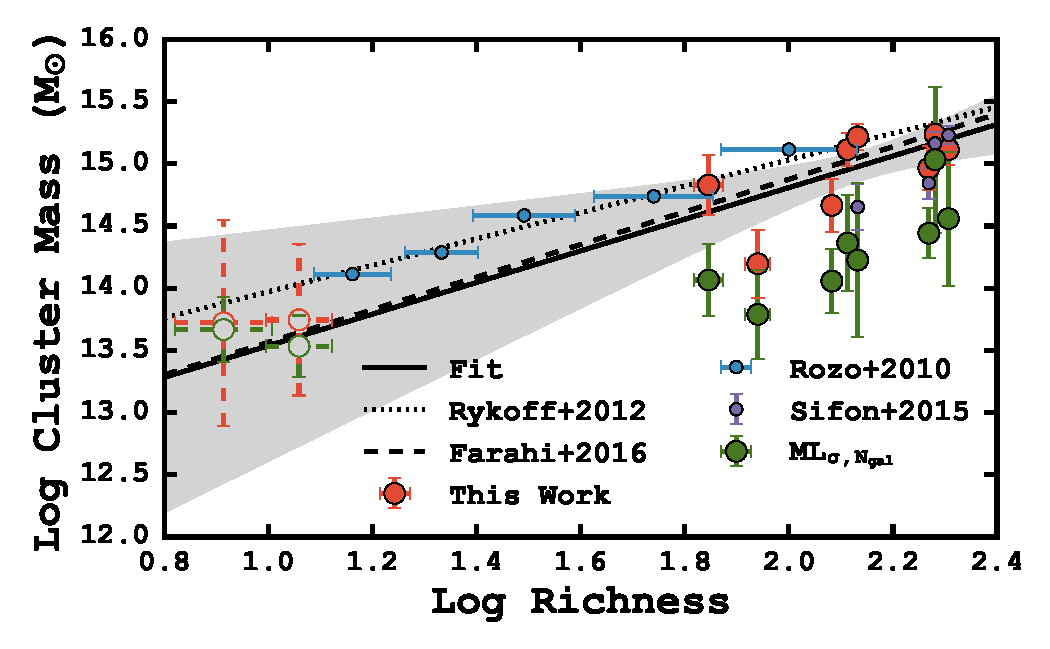
\includegraphics[width=\textwidth]{./figures2/massRichness.pdf} 
	\end{center}
	\caption[Richness, $\lambda$, versus total PL estimated cluster mass for the clusters in our sample.]{Richness, $\lambda$, versus total PL estimated cluster mass for the clusters in our sample. Our cluster mass measurements are shown as orange points. The two dashed points are the X-ray selected clusters, and are excluded from the fit. The solid black like shows our best-fitting relation (Equation~\protect\ref{2eq: best fit}) based on the eight high mass clusters, the dashed line shows the relation from \protect\cite{Farahi2016}, and the dotted line shows the relation from \protect\cite{Rykoff2012}. The gray shaded region corresponds to the 68\% confidence area on our best-fit. We include stacked WL masses from \protect\cite{Rozo2010}, the high-mass cluster mass estimates of \protect\cite{Sifon2015} and our $\mathrm{ML}_{\sigma, N_{gal}}$ predicted cluster masses for comparison.}
\label{2fig:massRichness} 
\end{figure}

In Section 2, we show that HETDEX will be able to accurately estimate the absolute calibration and intrinsic scatter, $\sigma_{M|\lambda}$, of the optical-richness-cluster-mass relationship for a small range of intrinsic scatters. Here we use the ten clusters observed to demonstrate the ability of IFU observations similar to HETDEX to make mass determinations and to use those masses to place constraints on the optical-richness-cluster-mass relation. For our cluster mass estimates we use the masses predicted by the PL relation given in Equation~\ref{2eq:power law}. 

To find a best-fitting richness-mass relation for our data we are required to fit $y=mx+b$ where $y =$ log predicted cluster mass and $x =$ log optical richness, considering measurement errors in richness and predicted cluster mass along with intrinsic scatter of the relation. We assume the intrinsic scatter is constant from point to point, and we assume (not necessarily correctly) that all measurement errors are Gaussian. With the assumption of all Gaussian scatters we have three quantities of interest:
The probability of the predicted log cluster mass ($y_i$) given the observed log richness ($x_i$),
\begin{equation}\label{2eqn:intrinsic scatter}
	p(y_i|x_i) = \frac{1}{\sqrt{2\,\pi\,\sigma^2}}
	 \,\exp\left(-\frac{[y_i - m\,x_i - b]^2}{2\,\sigma^2}\right)
\end{equation}
which takes into consideration the intrinsic scatter in the relation, $\sigma$; the probability of the true log richness value ($\hat{x_i}$) given an observed log richness ($x_i$),
\begin{equation}\label{2eqn:xerr}
	p(\hat{x_i}|x_i) = \frac{1}{\sqrt{2\,\pi\,\sigma_{x,i}^2}}
	 \,\exp\left(-\frac{[\hat{x_i} - x_i]^2}{2\,\sigma_{x,i}^2}\right)
\end{equation}
which accounts for the uncertainty in the richness observation, $\sigma_{x,i}$; and the probability of the true log cluster mass ($\hat{y_i}$) given an observed log cluster mass ($y_i$),
\begin{equation}\label{2eqn:yerr}
	p(\hat{y_i}|y_i) = \frac{1}{\sqrt{2\,\pi\,\sigma_{y,i}^2}}
	 \,\exp\left(-\frac{[\hat{y_i} -y_i]^2}{2\,\sigma_{y,i}^2}\right)
\end{equation}
which also considers the uncertainty associated with the log cluster mass prediction, $\sigma_{y,i}$. We combine these three probabilities into
\begin{equation}
	p(\hat{y_i}|\hat{x_i}) = \int_{-\infty}^\infty dy_ip(\hat{y_i}|y_i) \int_{-\infty}^\infty dx_ip(y_i|x_i)p(x_i|\hat{x_i}).
\end{equation}
We assume flat priors on $x_i$ so that $p(x_i|\hat{x_i}) = p(\hat{x_i}|x_i)$ and substitute our probability equations from above. This gives
\begin{equation}
	p(\hat{y_i}|\hat{x_i}) = 
	\frac{1}{\sqrt{2\,\pi\,(\sigma^2 + \sigma_{y,i}^2 + m^2\sigma_{x,i}^2)}}\exp\left(-\frac{[y_i - m\,x_i - b]^2}{2\,(\sigma^2 + \sigma_{y,i}^2 + m^2\sigma_{x,i}^2)}\right)
\end{equation}
which for $\sigma_{x,i}=0$ (no uncertainty on the log richness measurement) reduces to the familiar form of a Gaussian with a combination of measurement error and intrinsic scatter. We convert this probability function into a likelihood by taking the product of all the individual probabilities,  
\begin{equation}\label{2eq:like}
\mathscr{L} = \prod_{i=1}^N \ p(\hat{y_i}|\hat{x_i}).
\end{equation}
and maximize this likelihood by sampling from the posterior probability distribution using the MCMC methods described above. We quote the most probable slope and intercept as the mean value of the posterior probability distributions with uncertainties as the square root of the second moment of the same distribution.

To find our best-fitting relation we exclude the two \emph{XMM} selected clusters due to the few number of observed member galaxies. After fitting to the remaining eight, high richness clusters, we find a best-fitting relation of 
\begin{equation}\label{2eq: best fit}
 \mathrm{Log}\,M_{200c}/\Msol =1.25\pm{0.78}\, \mathrm{Log}\,\lambda + 12.29\pm{1.68}. 
\end{equation}
This best-fitting relation is shown in Figure~\ref{2fig:massRichness} where the large filled, orange points are the PL estimated cluster masses from this work, and the dashed points are the excluded \emph{XMM} selected clusters. We comment on the properties of our optical richness-mass relation and compare it to others from the literature in the following subsection.

We estimate the intrinsic scatter, $\sigma_{M|\lambda}$, in the relation two ways. The first is through our generative model, as it includes an intrinsic scatter term, which the MCMC samples directly. This gives $\sigma_{M|\lambda} = 0.23\pm0.16$ dex for the intrinsic scatter. We can also calculate the standard deviation of the residuals to the best-fitting line, which produces $\sigma_{M|\lambda} = 0.27\pm0.07$ dex. Both of these scatter estimates include the eight $\lambda > 60$ clusters. If we exclude MSJ215422.9+003723.5 where we significantly underestimate the mass when compared to literature values (see Subsection~\ref{2sec: Abell2392}), the scatter for remaining seven clusters is $\sigma_{M|\lambda} = 0.24\pm0.09$ dex.

\subsection{Calibration of the Richness-Mass Relation}
Two recent studies \citep{Farahi2016, Simet2016} use stacked cluster observations of velocity dispersions or WL, and it both cases report a PL index of $\alpha \sim 1.3$. We find a similar (6\% difference) PL index of $\alpha=1.25$, albeit with significant uncertainty. Our absolute mass scale of log $M_{200c}/\Msol = 14.29\pm2.1$ dex at $\lambda=40$ is in good agreement with the previously reported values of log $M_{200c}/\Msol = 14.34$ \citep{Simet2016} dex and log $M_{200c}/\Msol = 14.35$ \citep{Farahi2016} dex, although with much greater uncertainty. These large uncertainties are due to our sample have a low number of clusters; our fitting procedure cannot place tight constraints on the measured slope and intercept. With the many clusters expected to be observed with HETDEX these uncertainties should decrease significantly.

Our cluster masses estimates allow us to place promising constraints on the scatter in cluster mass at fixed richness, $\sigma_{M|\lambda}$. Using the SZE, \cite{Saro2015} find $\sigma_{M|\lambda} = 0.18$\err{0.08}{0.05} at $\lambda = 70$. \cite{Rykoff2016} identify a similar scatter of $0.3\pm0.15$ using X-ray scaling relations and the DES science verification dataset. Many other studies \citeeg{Baxter2016, Farahi2016, Simet2016} adopt a $\sigma_{M|\lambda}\sim 0.2-0.3$ dex \citep{Rozo2014, Rozo2015}. These values correspond well to our value of $\sigma_{M|\lambda} = 0.24\pm0.09$ dex, and the $0.2-0.3$ range corresponds well to the region most sensitively probed in our simulated HETDEX survey (Section 2).

The ability of blind spectroscopy to constrain both the absolute cluster mass scale and, more importantly, the amount of scatter at fixed optical richness to values similar to other techniques is extremely positive for the potential of HETDEX. As cluster mass estimates become better constrained through the use of ML methods, we can expect to find even tighter constrains on the optical richness-cluster mass relation. This should lead to excellent calibration of other large-area sky surveys which produce optical photometry only. In addition, it will serve as an important, independent check on other observable-cluster mass relationships which are often noisy and subjet to large systematic uncertainties \citeeg{Sereno2015}.

% \section{Summary}\label{2sec:summary}
% We carry out a proof-of-concept study where we present integral field unit observations with the Mitchelle Spectrograph of ten intermediate redshift ($z=0.2-0.3$) galaxy clusters. We observe cluster member galaxies within $R\sim0.5$ Mpc of each cluster, and determine each cluster's membership based on the line-of-sight velocity of each galaxy. The mass of each cluster is determined through a traditional PL and through a machine learning based approach. We use these estimates of cluster mass to measure the absolute mass scale and intrinsic scatter of the optical richness-cluster mass relationship. The goal of this study is to investigate how a blind spectroscopic survey, such as the forthcoming Hobby Eberly Dark Energy Experiment (HETDEX), will be able to predict cluster masses, and then to use those masses to help calibrate other observable-cluster mass scaling relations.
% Our main results are as follows:
% \begin{itemize}
% 	\item Using a PL scaling relation between the measured line-of-sight velocity dispersion and cluster mass, our low richness ($\lambda < 15$) sample of galaxy clusters have total inferred masses $\sim 0.5 \times 10^{14}$ \Msol\ ($M_{200c}$), and the high richness ($\lambda > 60$) cluster sample has total masses $(1.58-17.37) \times 10^{14}$ \Msol\ ($M_{200c}$). The majority of these estimate are consistent with other published total mass estimates which use a variety of estimation techniques.
%
% 	\item The machine learning based approach of galaxy cluster mass estimation, while powerful, requires a deep understanding of both the machine learning algorithms available, training sets that accurately represent the properties of the data, and expert knowledge of the problem domain. To estimate the total masses of the galaxy clusters in our sample using machine learning methods, the native Buzzard catalogs do not provide a suitable training set due to the limited cosmological volume simulated at low redshift. For the redshift range of our cluster sample, the Buzzard catalogs lack similar high line-of-sight velocity dispersion and high mass clusters. This leads to a severe down-weighting of high mass galaxy clusters when the cluster redshift is included as a training feature. When this feature is removed, the machine learning estimated cluster masses improve but are still underestimated due to too few very high mass clusters being included in the simulated volume. A suite of training data drawn from a similarly sized cosmological volume is critical to the reliable prediction of cluster masses. When this is available, the machine learning predicted cluster masses show less bias and lower scatter compared to a traditional power law scaling relation based on velocity dispersion alone.
%
% 	\item We fit a optical richness-cluster mass relation to the eight high richness ($\lambda > 60$) clusters. This gives:
% 		\begin{equation}
% 			\mathrm{Log}\,M_{200c}/\Msol=1.25\pm{0.78}\, \mathrm{Log}\,\lambda + 12.29\pm{1.68}.
% 		\end{equation}
% We are unable to place tight constraints on the overall estimate of the normalization due to the relatively few clusters included. We do estimate the scatter in cluster mass at fixed richness, $\sigma_{M|\lambda} \sim 0.25$. This estimate of scatter compares well with other recent studies of the richness-mass relation. This suggests that a blind spectroscopic survey such as HETDEX will be able to provide a crucial, independent measurement of this scatter, to a much high precision than is possible in this work. This bodes well for the success of HETDEX as not only a high redshift galaxy survey but as a important calibration tool for understanding the uncertainties associated with galaxy cluster mass estimates.
% \end{itemize}


%%%%%%%%%%%%%%%%%%%%%%%%%%%%%%%%%%%%%%%%%%%%%%%%%%%%%%%%%%%%%
\let\oldbibitem\bibitem 
\renewcommand{\bibitem}{\setlength{ 
\itemsep}{0pt}\oldbibitem}

%%%%%%%%%%%%%%%%%%%%%%%%%%%%%%%%%%%%%%%%%%%%%%%%%%%%%%%%%%%%%%%
%%%%%%%%%%%%%%%%%%%%%%%%%%%%%%%%%%%%%%%%%%%%%%%%%%%
%
%  New template code for TAMU Theses and Dissertations starting Fall 2012.  
%  For more info about this template or the 
%  TAMU LaTeX User's Group, see http://www.howdy.me/.
%
%  Author: Wendy Lynn Turner 
%	 Version 1.0X
%  Modified by Jimmy
%
%%%%%%%%%%%%%%%%%%%%%%%%%%%%%%%%%%%%%%%%%%%%%%%%%%%


%%%%%%%%%%%%%%%%%%%%%%%%%%%%%%%%%%%%%%%%%%%%%%%%%%%%%%%%%%%%%%%%%%%%%%
%%                           REFERENCES 
%%%%%%%%%%%%%%%%%%%%%%%%%%%%%%%%%%%%%%%%%%%%%%%%%%%%%%%%%%%%%%%%%%%%%

\phantomsection
\addcontentsline{toc}{chapter}{REFERENCES}

\renewcommand{\bibname}{{\normalsize\rm REFERENCES}}

\bibliographystyle{apj}
\bibliography{library}

%%%%%%%%%%%%%%%%%%%%%%%%%%%%%%%%%%%%%%%%%%%%%%%%%%%
%
%  New template code for TAMU Theses and Dissertations starting Fall 2012.  
%  For more info about this template or the 
%  TAMU LaTeX User's Group, see http://www.howdy.me/.
%
%  Author: Wendy Lynn Turner 
%	 Version 1.0 
%  Last updated 8/5/2012
%
%%%%%%%%%%%%%%%%%%%%%%%%%%%%%%%%%%%%%%%%%%%%%%%%%%%

\begin{appendices}
\titleformat{\chapter}{\centering\normalsize}{APPENDIX \thechapter}{0em}{\vskip .5\baselineskip\centering}
\renewcommand{\appendixname}{APPENDIX}

%%%%%%%%%%%%%%%%%%%%%%%%%%%%%%%%%%%%%%%%%%%%%%%%%%%
%
%  New template code for TAMU Theses and Dissertations starting Fall 2012.  
%  For more info about this template or the 
%  TAMU LaTeX User's Group, see http://www.howdy.me/.
%
%  Author: Wendy Lynn Turner 
%	 Version 1.0 
%  Last updated 8/5/2012
%
%%%%%%%%%%%%%%%%%%%%%%%%%%%%%%%%%%%%%%%%%%%%%%%%%%%

%%%%%%%%%%%%%%%%%%%%%%%%%%%%%%%%%%%%%%%%%%%%%%%%%%%%%%%%%%%%%%%%%%%%%%
%%                           APPENDIX A 
%%%%%%%%%%%%%%%%%%%%%%%%%%%%%%%%%%%%%%%%%%%%%%%%%%%%%%%%%%%%%%%%%%%%%

\phantomsection

\chapter{\uppercase{MS Observations}}

\begin{figure}
\begin{center}
	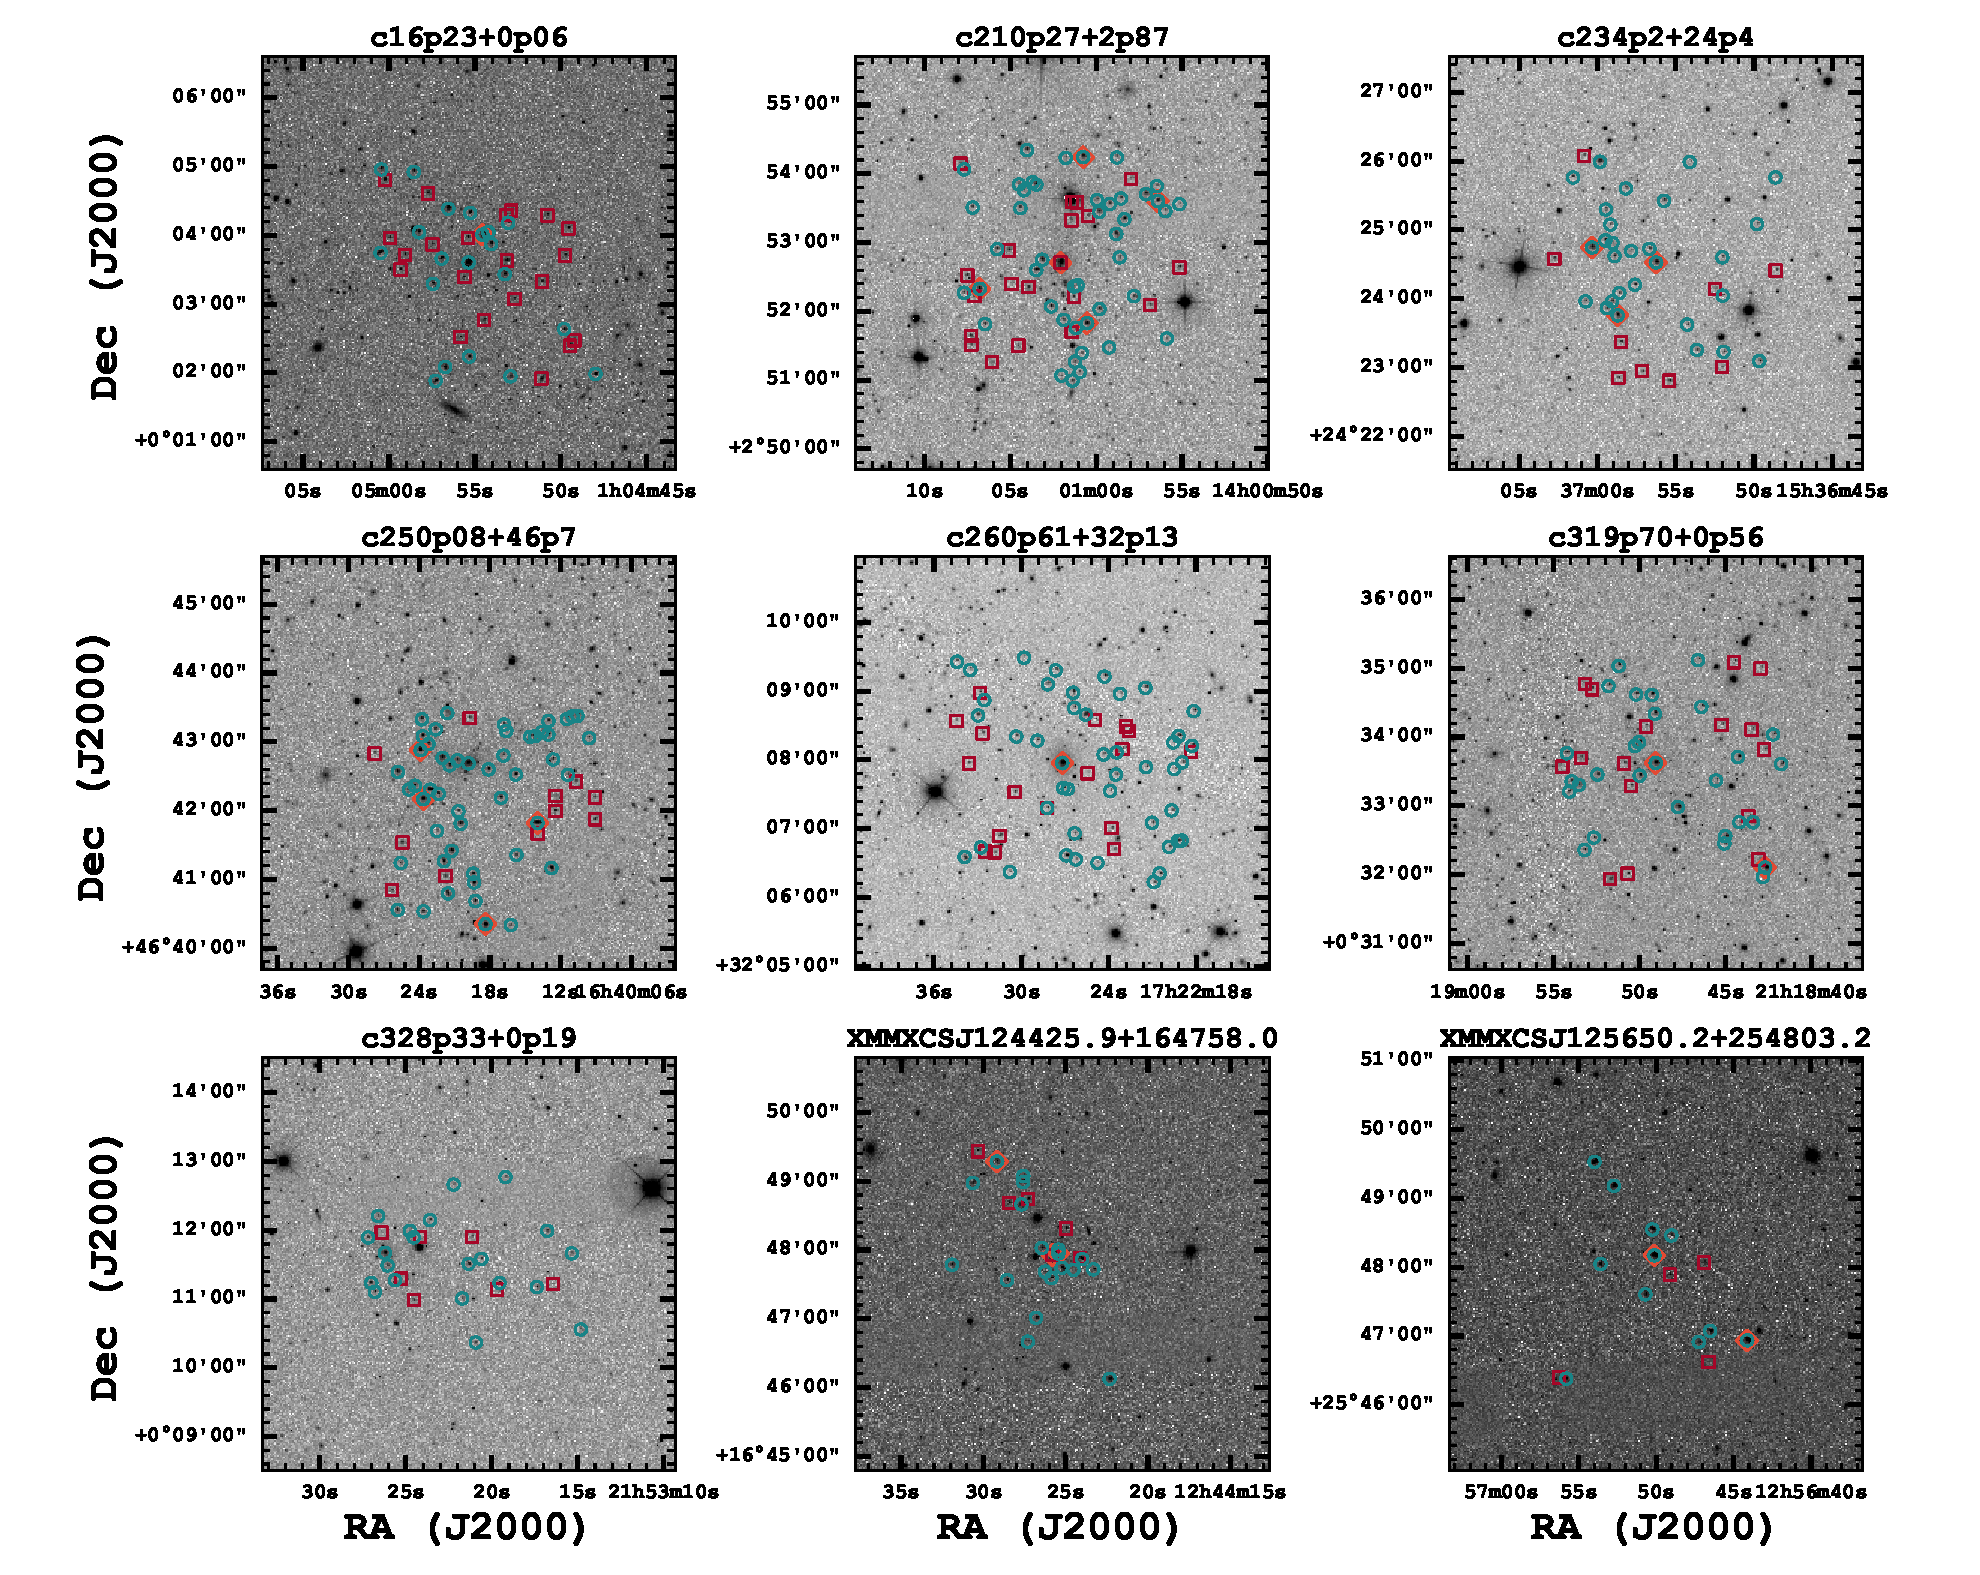
\includegraphics[width=\textwidth]{./figures2/multimontage.pdf}
\end{center}
	\caption[Montage of remaining nine clusters]{SDSS \sdssr\ image of cluster c203p83+41p0. The symbols show the position of observed galaxies. Blue circles indicate galaxies with $Q=0$ or $Q=1$ spectroscopic redshifts, red squares indicate galaxies where a redshift could not be reliably determined, and the orange diamond corresponds to galaxies with pre-existing redshifts from the SDSS. \textit{Right:} Example spectrum of an emission-line cluster galaxy (black line) and template fit (red line) from VIRUS-P on the McDonald 2.7m telescope. The spectrum shows the wavelength range and data quality expected from HETDEX-like spectroscopy, which are sufficient to measure galaxy redshifts.} 
	\label{2fig:montage}
\end{figure}


\begin{landscape}
	\begin{table}
		\centering 
		\caption[Spectroscopic redshifts for galaxies in MSJ010455.4+000336.3]{Spectroscopic redshifts for galaxies in MSJ010455.4+000336.3 measured with the MS: Columns as in Table~\ref{2tbl:MSJ133520.1+410004.1}.}
		\begin{tabular}{ccccccccccc}
			\hline
			tile & dither & fiber & ra & dec & r (mag) & redshift & Q & Member & R (Mpc) & LOSV (\kms) \\
			(1) & (2) & (3) & (4) & (5) & (6) & (7) & (8) & (9) & (10) & (11) \\
			\hline \hline
			NE & 1 & 223 & 01:04:56.937 & +00:03:39.60 & 19.38 & 0.2691$\pm{0.0002}$ & 0 & $\checkmark$ & 0.10 & -748$\pm{89}$ \\
			NE & 2 & 42 & 01:05:00.449 & +00:04:57.41 & 19.80 & 0.2766$\pm{0.0001}$ & 1 & $\checkmark$ & 0.47 & 1005$\pm{52}$ \\
			NE & 2 & 168 & 01:04:58.247 & +00:04:02.62 & 19.75 & 0.3054$\pm{0.0003}$ & 1 & ... & 0.23 & 7783$\pm{122}$ \\
			NE & 2 & 216 & 01:05:00.487 & +00:03:44.70 & 18.85 & 0.0826$\pm{0.0004}$ & 1 & ... & 0.12 & -44576$\pm{193}$ \\
			NE & 2 & 220 & 01:04:55.367 & +00:03:36.34 & 17.27 & 0.2715$\pm{0.0001}$ & 0 & $\checkmark$ & 0.00 & -193$\pm{61}$ \\
			NE & 3 & 38 & 01:04:58.559 & +00:04:55.13 & 19.95 & 0.3510$\pm{0.0001}$ & 1 & ... & 0.46 & 18494$\pm{56}$ \\
			NE & 3 & 106 & 01:04:56.545 & +00:04:23.15 & 18.36 & 0.2788$\pm{0.0001}$ & 0 & $\checkmark$ & 0.21 & 1517$\pm{47}$ \\
			NE & 3 & 118 & 01:04:55.276 & +00:04:19.53 & 19.49 & 0.2747$\pm{0.0001}$ & 0 & $\checkmark$ & 0.18 & 566$\pm{71}$ \\
			NE & 3 & 160 & 01:04:54.563 & +00:04:00.66 & 18.19 & 0.2747$\pm{0.0001}$ & 0 & $\checkmark$ & 0.11 & 559$\pm{52}$ \\
			NW & 1 & 156 & 01:04:53.064 & +00:04:10.99 & 20.22 & 0.2234$\pm{0.0001}$ & 1 & ... & 0.18 & -11495$\pm{52}$ \\
			NW & 2 & 173 & 01:04:54.217 & +00:04:02.78 & 19.62 & 0.2629$\pm{0.0002}$ & 0 & $\checkmark$ & 0.13 & -2205$\pm{80}$ \\
			NW & 3 & 187 & 01:04:54.051 & +00:03:52.42 & 19.35 & 0.3290$\pm{0.0001}$ & 1 & ... & 0.12 & 13319$\pm{52}$ \\
			SE & 1 & 50 & 01:04:57.440 & +00:03:17.71 & 19.51 & 0.2718$\pm{0.0002}$ & 1 & $\checkmark$ & 0.15 & -123$\pm{75}$ \\
			SE & 2 & 191 & 01:04:55.332 & +00:02:14.18 & 19.79 & 0.2794$\pm{0.0001}$ & 0 & $\checkmark$ & 0.35 & 1658$\pm{66}$ \\
			SE & 3 & 208 & 01:04:56.734 & +00:02:05.07 & 18.75 & 0.2781$\pm{0.0001}$ & 0 & $\checkmark$ & 0.40 & 1358$\pm{42}$ \\
			SE & 3 & 238 & 01:04:57.284 & +00:01:53.04 & 19.58 & 0.2705$\pm{0.0001}$ & 0 & $\checkmark$ & 0.45 & -421$\pm{66}$ \\
			SW & 2 & 26 & 01:04:53.268 & +00:03:26.04 & 18.99 & 0.2666$\pm{0.0002}$ & 0 & $\checkmark$ & 0.14 & -1352$\pm{85}$ \\
			SW & 2 & 135 & 01:04:49.814 & +00:02:38.18 & 20.10 & 0.2697$\pm{0.0002}$ & 1 & $\checkmark$ & 0.42 & -619$\pm{85}$ \\
			SW & 2 & 218 & 01:04:47.988 & +00:01:59.05 & 19.55 & 0.2627$\pm{0.0001}$ & 1 & $\checkmark$ & 0.60 & -2259$\pm{42}$ \\
			SW & 3 & 228 & 01:04:52.934 & +00:01:56.95 & 20.37 & 0.2763$\pm{0.0001}$ & 1 & $\checkmark$ & 0.45 & 928$\pm{47}$ \\
			\hline
		\end{tabular}
		\label{2tbl:MSJ010455.4+000336.3}
	\end{table}
\end{landscape}


\begin{landscape}
	\singlespace
	\begin{longtable}{ccccccccccc}
	\caption[Spectroscopic redshifts for galaxies in MSJ153656.3+242431.6]{Spectroscopic redshifts for galaxies in MSJ153656.3+242431.6 measured with the MS: Columns as in Table~\ref{2tbl:MSJ133520.1+410004.1}}\\
	\hline
	tile & dither & fiber & ra & dec & r (mag) & redshift & Q & Member & R (Mpc) & LOSV (\kms) \\
	(1) & (2) & (3) & (4) & (5) & (6) & (7) & (8) & (9) & (10) & (11) \\
	\hline \hline
	\endfirsthead
	\multicolumn{4}{l}%
	{\tablename\ \thetable\ Continued} \\
	\hline
	tile & dither & fiber & ra & dec & r (mag) & redshift & Q & Member & R (Mpc) & LOSV (\kms) \\
	(1) & (2) & (3) & (4) & (5) & (6) & (7) & (8) & (9) & (10) & (11) \\
	\hline \hline
	\endhead
	NE & 1 & 78 & 15:36:58.192 & +24:25:36.14 & 19.81 & 0.3228$\pm{0.0001}$ & 0 & ... & 0.33 & 23652$\pm{44}$ \\
	NE & 1 & 124 & 15:36:59.468 & +24:25:17.76 & 19.83 & 0.2324$\pm{0.0004}$ & 1 & $\checkmark$ & 0.24 & 1609$\pm{195}$ \\
	NE & 1 & 208 & 15:36:57.848 & +24:24:41.47 & 20.35 & 0.1881$\pm{0.0001}$ & 0 & ... & 0.08 & -9197$\pm{34}$ \\
	NE & 2 & 11 & 15:37:00.861 & +24:26:04.40 & 20.48 & 0.0947$\pm{0.0001}$ & 1 & ... & 0.20 & -31965$\pm{54}$ \\
	NE & 2 & 153 & 15:36:59.174 & +24:25:04.55 & 20.37 & 0.1036$\pm{0.0002}$ & 1 & ... & 0.10 & -29809$\pm{98}$ \\
	NE & 2 & 232 & 15:37:02.759 & +24:24:34.63 & 19.98 & 0.3017$\pm{0.0001}$ & 1 & ... & 0.40 & 18513$\pm{49}$ \\
	NE & 3 & 23 & 15:36:59.839 & +24:25:59.51 & 18.05 & 0.1275$\pm{0.0000}$ & 0 & ... & 0.23 & -23979$\pm{20}$ \\
	NE & 3 & 55 & 15:37:01.554 & +24:25:45.67 & 19.79 & 0.2115$\pm{0.0001}$ & 1 & ... & 0.36 & -3477$\pm{49}$ \\
	NE & 3 & 181 & 15:36:59.035 & +24:24:48.56 & 20.11 & 0.1874$\pm{0.0001}$ & 1 & ... & 0.13 & -9363$\pm{39}$ \\
	NE & 3 & 182 & 15:36:59.498 & +24:24:50.78 & 19.62 & 0.1231$\pm{0.0003}$ & 1 & ... & 0.11 & -25050$\pm{151}$ \\
	NE & 3 & 191 & 15:36:56.681 & +24:24:43.40 & 19.54 & 0.1808$\pm{0.0000}$ & 0 & ... & 0.04 & -10980$\pm{24}$ \\
	NE & 3 & 198 & 15:37:00.334 & +24:24:44.60 & 17.27 & 0.2274$\pm{0.0002}$ & 0 & $\checkmark$ & 0.21 & 387$\pm{112}$ \\
	NE & 3 & 210 & 15:36:58.911 & +24:24:37.07 & 19.67 & 0.4813$\pm{0.0000}$ & 1 & ... & 0.22 & 62324$\pm{24}$ \\
	NE & 3 & 219 & 15:36:56.253 & +24:24:31.59 & 17.36 & 0.2262$\pm{0.0001}$ & 0 & $\checkmark$ & 0.00 & 94$\pm{63}$ \\
	NW & 1 & 116 & 15:36:55.756 & +24:25:25.38 & 18.90 & 0.2706$\pm{0.0001}$ & 1 & ... & 0.23 & 10924$\pm{49}$ \\
	NW & 1 & 148 & 15:36:49.817 & +24:25:04.96 & 20.02 & 0.2224$\pm{0.0001}$ & 0 & $\checkmark$ & 0.34 & -813$\pm{63}$ \\
	NW & 2 & 26 & 15:36:54.106 & +24:25:59.10 & 20.79 & 0.2298$\pm{0.0000}$ & 0 & $\checkmark$ & 0.34 & 972$\pm{24}$ \\
	NW & 3 & 44 & 15:36:48.628 & +24:25:45.78 & 21.29 & 0.3341$\pm{0.0001}$ & 1 & ... & 0.62 & 26416$\pm{59}$ \\
	NW & 3 & 210 & 15:36:52.024 & +24:24:36.09 & 19.78 & 0.2281$\pm{0.0001}$ & 0 & $\checkmark$ & 0.21 & 570$\pm{63}$ \\
	SE & 1 & 48 & 15:36:57.612 & +24:24:12.18 & 19.43 & 0.2215$\pm{0.0002}$ & 0 & $\checkmark$ & 0.10 & -1038$\pm{78}$ \\
	SE & 1 & 64 & 15:36:58.605 & +24:24:04.80 & 20.06 & 0.2124$\pm{0.0001}$ & 1 & ... & 0.15 & -3277$\pm{59}$ \\
	SE & 2 & 80 & 15:36:59.058 & +24:23:57.63 & 19.24 & 0.2280$\pm{0.0002}$ & 0 & $\checkmark$ & 0.19 & 528$\pm{93}$ \\
	SE & 2 & 95 & 15:36:59.393 & +24:23:51.85 & 19.35 & 0.1244$\pm{0.0002}$ & 1 & ... & 0.13 & -24730$\pm{98}$ \\
	SE & 3 & 108 & 15:36:58.708 & +24:23:45.47 & 17.70 & 0.2235$\pm{0.0002}$ & 0 & $\checkmark$ & 0.21 & -565$\pm{83}$ \\
	SW & 1 & 66 & 15:36:52.487 & +24:24:08.35 & 20.29 & 0.1248$\pm{0.0001}$ & 1 & ... & 0.13 & -24633$\pm{63}$ \\
	SW & 1 & 142 & 15:36:54.270 & +24:23:37.37 & 20.15 & 0.2546$\pm{0.0001}$ & 0 & ... & 0.24 & 7019$\pm{54}$ \\
	SW & 2 & 185 & 15:36:53.657 & +24:23:15.33 & 19.58 & 0.2239$\pm{0.0002}$ & 0 & $\checkmark$ & 0.30 & -450$\pm{98}$ \\
	SW & 3 & 65 & 15:36:51.996 & +24:24:02.62 & 20.31 & 0.2201$\pm{0.0001}$ & 1 & $\checkmark$ & 0.23 & -1382$\pm{34}$ \\
	\hline
	\label{2tbl:MSJ153656.3+242431.6}
	\end{longtable}
\end{landscape}


\begin{landscape}
	\singlespace
	\begin{longtable}{ccccccccccc}
	\caption[Spectroscopic redshifts for galaxies in MSJ164019.8+464241.5]{Spectroscopic redshifts for galaxies in MSJ164019.8+464241.5 measured with the MS: Columns as in Table~\ref{2tbl:MSJ133520.1+410004.1}.}\\
	\hline
	tile & dither & fiber & ra & dec & r (mag) & redshift & Q & Member & R (Mpc) & LOSV (\kms) \\
	(1) & (2) & (3) & (4) & (5) & (6) & (7) & (8) & (9) & (10) & (11) \\
	\hline \hline
	\endfirsthead
	\multicolumn{4}{l}%
	{\tablename\ \thetable\ Continued} \\
	\hline
	tile & dither & fiber & ra & dec & r (mag) & redshift & Q & Member & R (Mpc) & LOSV (\kms) \\
	(1) & (2) & (3) & (4) & (5) & (6) & (7) & (8) & (9) & (10) & (11) \\
	\hline \hline
	\endhead
	NE & 1 & 34 & 16:40:21.617 & +46:43:25.07 & 20.12 & 0.1014$\pm{0.0003}$ & 0 & ... & 0.09 & -30528$\pm{141}$ \\
	NE & 1 & 110 & 16:40:23.879 & +46:42:52.76 & 17.81 & 0.2333$\pm{0.0000}$ & 0 & $\checkmark$ & 0.16 & 1617$\pm{24}$ \\
	NE & 1 & 133 & 16:40:19.812 & +46:42:41.30 & 16.61 & 0.2238$\pm{0.0001}$ & 0 & $\checkmark$ & 0.00 & -699$\pm{39}$ \\
	NE & 1 & 156 & 16:40:25.818 & +46:42:33.87 & 18.36 & 0.2099$\pm{0.0001}$ & 0 & ... & 0.21 & -4092$\pm{54}$ \\
	NE & 1 & 183 & 16:40:24.352 & +46:42:21.79 & 19.33 & 0.2248$\pm{0.0002}$ & 0 & $\checkmark$ & 0.18 & -462$\pm{93}$ \\
	NE & 1 & 211 & 16:40:23.651 & +46:42:10.01 & 17.62 & 0.2287$\pm{0.0001}$ & 0 & $\checkmark$ & 0.19 & 483$\pm{39}$ \\
	NE & 2 & 65 & 16:40:22.597 & +46:43:10.93 & 19.73 & 0.1813$\pm{0.0002}$ & 1 & ... & 0.13 & -11053$\pm{88}$ \\
	NE & 2 & 81 & 16:40:23.696 & +46:43:04.86 & 18.62 & 0.2324$\pm{0.0001}$ & 0 & $\checkmark$ & 0.17 & 1400$\pm{68}$ \\
	NE & 2 & 95 & 16:40:23.219 & +46:42:58.04 & 19.32 & 0.2264$\pm{0.0001}$ & 0 & $\checkmark$ & 0.14 & -75$\pm{39}$ \\
	NE & 2 & 122 & 16:40:22.018 & +46:42:46.03 & 18.84 & 0.2079$\pm{0.0001}$ & 0 & ... & 0.08 & -4574$\pm{73}$ \\
	NE & 2 & 136 & 16:40:21.428 & +46:42:39.59 & 19.11 & 0.2180$\pm{0.0002}$ & 0 & $\checkmark$ & 0.06 & -2120$\pm{93}$ \\
	NE & 2 & 195 & 16:40:22.346 & +46:42:14.63 & 19.21 & 0.2289$\pm{0.0002}$ & 0 & $\checkmark$ & 0.14 & 542$\pm{93}$ \\
	NE & 3 & 37 & 16:40:23.777 & +46:43:19.71 & 19.22 & 0.2229$\pm{0.0002}$ & 0 & $\checkmark$ & 0.20 & -933$\pm{102}$ \\
	NE & 3 & 120 & 16:40:20.755 & +46:42:43.96 & 17.82 & 0.2216$\pm{0.0002}$ & 0 & $\checkmark$ & 0.04 & -1240$\pm{83}$ \\
	NE & 3 & 181 & 16:40:23.067 & +46:42:18.32 & 18.39 & 0.2191$\pm{0.0001}$ & 0 & $\checkmark$ & 0.14 & -1852$\pm{39}$ \\
	NE & 3 & 184 & 16:40:24.861 & +46:42:18.39 & 19.09 & 0.2110$\pm{0.0002}$ & 0 & ... & 0.20 & -3816$\pm{78}$ \\
	NW & 1 & 50 & 16:40:13.038 & +46:43:18.14 & 19.37 & 0.2289$\pm{0.0002}$ & 0 & $\checkmark$ & 0.29 & 539$\pm{78}$ \\
	NW & 1 & 79 & 16:40:13.042 & +46:43:06.31 & 19.12 & 0.2297$\pm{0.0001}$ & 0 & $\checkmark$ & 0.27 & 730$\pm{34}$ \\
	NW & 1 & 81 & 16:40:14.572 & +46:43:04.50 & 20.49 & 0.2249$\pm{0.0002}$ & 1 & $\checkmark$ & 0.21 & -443$\pm{102}$ \\
	NW & 1 & 128 & 16:40:16.854 & +46:42:48.04 & 20.31 & 0.2281$\pm{0.0001}$ & 1 & $\checkmark$ & 0.11 & 342$\pm{68}$ \\
	NW & 1 & 215 & 16:40:17.060 & +46:42:11.27 & 19.21 & 0.2580$\pm{0.0002}$ & 1 & ... & 0.17 & 7632$\pm{122}$ \\
	NW & 2 & 33 & 16:40:10.991 & +46:43:22.18 & 19.33 & 0.2228$\pm{0.0001}$ & 1 & $\checkmark$ & 0.36 & -940$\pm{49}$ \\
	NW & 2 & 56 & 16:40:16.794 & +46:43:15.13 & 20.91 & 0.2350$\pm{0.0001}$ & 1 & $\checkmark$ & 0.17 & 2021$\pm{73}$ \\
	NW & 2 & 70 & 16:40:16.608 & +46:43:09.56 & 20.70 & 0.2167$\pm{0.0002}$ & 1 & $\checkmark$ & 0.15 & -2427$\pm{88}$ \\
	NW & 2 & 81 & 16:40:14.180 & +46:43:05.00 & 19.20 & 0.2252$\pm{0.0001}$ & 0 & $\checkmark$ & 0.23 & -375$\pm{68}$ \\
	NW & 2 & 156 & 16:40:15.807 & +46:42:31.47 & 18.88 & 0.2281$\pm{0.0002}$ & 0 & $\checkmark$ & 0.16 & 344$\pm{83}$ \\
	NW & 3 & 33 & 16:40:11.463 & +46:43:19.95 & 19.11 & 0.2249$\pm{0.0002}$ & 0 & $\checkmark$ & 0.34 & -426$\pm{97}$ \\
	NW & 3 & 65 & 16:40:13.553 & +46:43:08.81 & 20.49 & 0.1319$\pm{0.0001}$ & 1 & ... & 0.16 & -23097$\pm{29}$ \\
	NW & 3 & 74 & 16:40:09.583 & +46:43:03.29 & 20.34 & 0.1735$\pm{0.0001}$ & 1 & ... & 0.32 & -12967$\pm{58}$ \\
	NW & 3 & 122 & 16:40:12.635 & +46:42:44.68 & 19.66 & 0.2270$\pm{0.0001}$ & 0 & $\checkmark$ & 0.27 & 79$\pm{63}$ \\
	NW & 3 & 144 & 16:40:18.116 & +46:42:35.97 & 19.27 & 0.2080$\pm{0.0002}$ & 1 & ... & 0.06 & -4567$\pm{102}$ \\
	NW & 3 & 149 & 16:40:11.390 & +46:42:31.31 & 20.02 & 0.0844$\pm{0.0002}$ & 1 & ... & 0.14 & -34675$\pm{88}$ \\
	SE & 1 & 4 & 16:40:20.674 & +46:41:59.40 & 20.48 & 0.2341$\pm{0.0001}$ & 0 & $\checkmark$ & 0.16 & 1797$\pm{54}$ \\
	SE & 1 & 50 & 16:40:22.486 & +46:41:42.33 & 20.51 & 0.2376$\pm{0.0002}$ & 1 & ... & 0.25 & 2670$\pm{78}$ \\
	SE & 1 & 107 & 16:40:21.903 & +46:41:15.96 & 18.82 & 0.1866$\pm{0.0001}$ & 0 & ... & 0.28 & -9766$\pm{58}$ \\
	SE & 1 & 147 & 16:40:19.343 & +46:40:57.31 & 18.39 & 0.1864$\pm{0.0001}$ & 0 & ... & 0.33 & -9815$\pm{34}$ \\
	SE & 1 & 211 & 16:40:23.625 & +46:40:32.22 & 19.06 & 0.2325$\pm{0.0001}$ & 0 & $\checkmark$ & 0.50 & 1410$\pm{54}$ \\
	SE & 1 & 214 & 16:40:25.819 & +46:40:33.21 & 19.03 & 0.2272$\pm{0.0002}$ & 0 & $\checkmark$ & 0.52 & 113$\pm{93}$ \\
	SE & 2 & 113 & 16:40:25.565 & +46:41:14.28 & 20.51 & 0.2221$\pm{0.0002}$ & 0 & $\checkmark$ & 0.38 & -1116$\pm{83}$ \\
	SE & 2 & 165 & 16:40:21.553 & +46:40:47.83 & 18.59 & 0.2110$\pm{0.0001}$ & 1 & ... & 0.40 & -3819$\pm{68}$ \\
	SE & 3 & 18 & 16:40:20.484 & +46:41:48.57 & 18.80 & 0.2347$\pm{0.0001}$ & 0 & $\checkmark$ & 0.20 & 1960$\pm{58}$ \\
	SE & 3 & 77 & 16:40:21.250 & +46:41:25.01 & 18.21 & 0.1892$\pm{0.0001}$ & 0 & ... & 0.25 & -9128$\pm{29}$ \\
	SE & 3 & 118 & 16:40:19.417 & +46:41:05.03 & 19.40 & 0.2238$\pm{0.0002}$ & 0 & $\checkmark$ & 0.35 & -701$\pm{102}$ \\
	SE & 3 & 176 & 16:40:19.231 & +46:40:41.13 & 19.36 & 0.2167$\pm{0.0001}$ & 0 & ... & 0.42 & -2444$\pm{39}$ \\
	SW & 1 & 122 & 16:40:12.787 & +46:41:09.93 & 18.22 & 0.2340$\pm{0.0001}$ & 0 & $\checkmark$ & 0.44 & 1785$\pm{34}$ \\
	SW & 1 & 243 & 16:40:16.232 & +46:40:20.20 & 20.28 & 0.2278$\pm{0.0002}$ & 1 & $\checkmark$ & 0.53 & 274$\pm{88}$ \\
	SW & 1 & 246 & 16:40:18.377 & +46:40:20.93 & 17.51 & 0.1874$\pm{0.0002}$ & 0 & ... & 0.44 & -9576$\pm{107}$ \\
	SW & 2 & 98 & 16:40:15.754 & +46:41:21.37 & 20.03 & 0.2243$\pm{0.0001}$ & 0 & $\checkmark$ & 0.33 & -572$\pm{63}$ \\
	SW & 3 & 22 & 16:40:13.962 & +46:41:49.44 & 17.63 & 0.1107$\pm{0.0001}$ & 0 & ... & 0.16 & -28264$\pm{54}$ \\
	\hline
	\label{2tbl:MSJ164019.8+464241.5}
	\end{longtable}
\end{landscape}


\begin{landscape}
	\singlespace
	\begin{longtable}{ccccccccccc}
	\caption[Spectroscopic redshifts for galaxies in MSJ140102.0+025242.6]{Spectroscopic redshifts for galaxies in MSJ140102.0+025242.6 measured with the MS: Columns as in Table~\ref{2tbl:MSJ133520.1+410004.1}}\\
	\hline
	tile & dither & fiber & ra & dec & r (mag) & redshift & Q & Member & R (Mpc) & LOSV (\kms) \\
	(1) & (2) & (3) & (4) & (5) & (6) & (7) & (8) & (9) & (10) & (11) \\
	\hline \hline
	\endfirsthead
	\multicolumn{4}{l}%
	{\tablename\ \thetable\ Continued} \\
	\hline
	tile & dither & fiber & ra & dec & r (mag) & redshift & Q & Member & R (Mpc) & LOSV (\kms) \\
	(1) & (2) & (3) & (4) & (5) & (6) & (7) & (8) & (9) & (10) & (11) \\
	\hline \hline
	\endhead
	NE & 1 & 6 & 14:01:04.022 & +02:54:20.65 & 19.01 & 0.2478$\pm{0.0002}$ & 0 & $\checkmark$ & 0.40 & -1626$\pm{81}$ \\
	NE & 1 & 16 & 14:01:01.771 & +02:54:13.80 & 20.37 & 0.3158$\pm{0.0002}$ & 1 & ... & 0.42 & 14574$\pm{81}$ \\
	NE & 1 & 123 & 14:01:04.410 & +02:53:29.95 & 19.70 & 0.2325$\pm{0.0002}$ & 1 & ... & 0.22 & -5275$\pm{119}$ \\
	NE & 2 & 43 & 14:01:07.682 & +02:54:03.80 & 20.20 & 0.2039$\pm{0.0001}$ & 1 & ... & 0.40 & -12093$\pm{33}$ \\
	NE & 2 & 64 & 14:01:03.691 & +02:53:52.63 & 20.48 & 0.2876$\pm{0.0002}$ & 1 & ... & 0.32 & 7854$\pm{110}$ \\
	NE & 2 & 222 & 14:01:03.134 & +02:52:45.00 & 18.66 & 0.2517$\pm{0.0002}$ & 0 & $\checkmark$ & 0.07 & -699$\pm{91}$ \\
	NE & 3 & 63 & 14:01:03.475 & +02:53:50.51 & 18.68 & 0.2598$\pm{0.0002}$ & 0 & $\checkmark$ & 0.29 & 1217$\pm{110}$ \\
	NE & 3 & 65 & 14:01:04.494 & +02:53:50.70 & 20.31 & 0.2540$\pm{0.0002}$ & 0 & $\checkmark$ & 0.31 & -149$\pm{86}$ \\
	NE & 3 & 79 & 14:01:04.203 & +02:53:45.54 & 20.26 & 0.2192$\pm{0.0001}$ & 1 & ... & 0.25 & -8444$\pm{67}$ \\
	NE & 3 & 114 & 14:01:07.185 & +02:53:30.54 & 20.11 & 0.2606$\pm{0.0002}$ & 1 & $\checkmark$ & 0.37 & 1405$\pm{81}$ \\
	NE & 3 & 198 & 14:01:05.757 & +02:52:54.15 & 19.70 & 0.2516$\pm{0.0002}$ & 0 & $\checkmark$ & 0.23 & -737$\pm{114}$ \\
	NE & 3 & 237 & 14:01:03.483 & +02:52:35.96 & 18.94 & 0.3110$\pm{0.0001}$ & 1 & ... & 0.11 & 13416$\pm{52}$ \\
	NW & 1 & 23 & 14:00:58.786 & +02:54:14.18 & 20.07 & 0.2318$\pm{0.0001}$ & 1 & ... & 0.38 & -5458$\pm{71}$ \\
	NW & 1 & 92 & 14:00:57.098 & +02:53:42.10 & 18.42 & 0.2108$\pm{0.0002}$ & 0 & ... & 0.32 & -10444$\pm{119}$ \\
	NW & 1 & 105 & 14:00:56.404 & +02:53:36.25 & 18.55 & 0.2504$\pm{0.0002}$ & 0 & $\checkmark$ & 0.39 & -1030$\pm{91}$ \\
	NW & 1 & 111 & 14:00:59.191 & +02:53:33.62 & 19.78 & 0.2458$\pm{0.0002}$ & 0 & $\checkmark$ & 0.25 & -2108$\pm{105}$ \\
	NW & 2 & 103 & 14:00:55.146 & +02:53:33.41 & 21.44 & 0.1642$\pm{0.0003}$ & 1 & ... & 0.32 & -21563$\pm{143}$ \\
	NW & 2 & 119 & 14:00:55.968 & +02:53:27.36 & 20.34 & 0.3084$\pm{0.0003}$ & 1 & ... & 0.46 & 12808$\pm{129}$ \\
	NW & 2 & 127 & 14:00:59.815 & +02:53:26.69 & 19.29 & 0.2723$\pm{0.0001}$ & 1 & ... & 0.23 & 4205$\pm{38}$ \\
	NW & 3 & 13 & 14:01:00.752 & +02:54:14.53 & 17.96 & 0.2492$\pm{0.0002}$ & 1 & $\checkmark$ & 0.37 & -1312$\pm{81}$ \\
	NW & 3 & 62 & 14:00:56.466 & +02:53:49.12 & 20.53 & 0.3932$\pm{0.0001}$ & 1 & ... & 0.57 & 33012$\pm{67}$ \\
	NW & 3 & 95 & 14:00:58.558 & +02:53:38.37 & 20.03 & 0.2363$\pm{0.0001}$ & 1 & ... & 0.28 & -4369$\pm{48}$ \\
	NW & 3 & 98 & 14:00:59.942 & +02:53:37.00 & 20.63 & 0.4784$\pm{0.0000}$ & 1 & ... & 0.37 & 53304$\pm{24}$ \\
	NW & 3 & 138 & 14:00:58.352 & +02:53:20.29 & 18.69 & 0.2557$\pm{0.0002}$ & 0 & $\checkmark$ & 0.26 & 245$\pm{100}$ \\
	NW & 3 & 168 & 14:00:58.824 & +02:53:07.37 & 18.61 & 0.2321$\pm{0.0001}$ & 0 & ... & 0.20 & -5375$\pm{67}$ \\
	NW & 3 & 211 & 14:00:58.625 & +02:52:47.07 & 20.02 & 0.1463$\pm{0.0002}$ & 1 & ... & 0.13 & -25817$\pm{86}$ \\
	SE & 1 & 90 & 14:01:02.616 & +02:52:04.19 & 19.19 & 0.2639$\pm{0.0002}$ & 1 & $\checkmark$ & 0.16 & 2201$\pm{91}$ \\
	SE & 1 & 234 & 14:01:02.016 & +02:51:03.83 & 21.20 & 0.2830$\pm{0.0002}$ & 1 & ... & 0.42 & 6738$\pm{86}$ \\
	SE & 2 & 56 & 14:01:06.778 & +02:52:19.68 & 17.90 & 0.2249$\pm{0.0002}$ & 1 & ... & 0.27 & -7098$\pm{76}$ \\
	SE & 2 & 72 & 14:01:07.685 & +02:52:16.24 & 20.08 & 0.3193$\pm{0.0002}$ & 0 & ... & 0.42 & 15401$\pm{81}$ \\
	SE & 3 & 103 & 14:01:01.894 & +02:51:52.53 & 19.80 & 0.2437$\pm{0.0001}$ & 1 & $\checkmark$ & 0.19 & -2625$\pm{67}$ \\
	SE & 3 & 127 & 14:01:06.471 & +02:51:48.78 & 19.58 & 0.2726$\pm{0.0001}$ & 1 & ... & 0.36 & 4284$\pm{71}$ \\
	SW & 1 & 57 & 14:01:01.072 & +02:52:22.71 & 20.15 & 0.1615$\pm{0.0002}$ & 0 & ... & 0.07 & -22207$\pm{91}$ \\
	SW & 1 & 144 & 14:01:01.183 & +02:51:45.62 & 20.01 & 0.2670$\pm{0.0002}$ & 0 & $\checkmark$ & 0.24 & 2930$\pm{119}$ \\
	SW & 2 & 58 & 14:01:01.278 & +02:52:21.62 & 20.96 & 0.2581$\pm{0.0001}$ & 1 & $\checkmark$ & 0.09 & 821$\pm{57}$ \\
	SW & 2 & 65 & 14:00:57.802 & +02:52:13.21 & 20.18 & 0.4127$\pm{0.0002}$ & 1 & ... & 0.38 & 37664$\pm{86}$ \\
	SW & 2 & 98 & 14:00:59.802 & +02:52:01.88 & 19.31 & 0.2549$\pm{0.0002}$ & 1 & $\checkmark$ & 0.21 & 49$\pm{105}$ \\
	SW & 2 & 148 & 14:00:55.880 & +02:51:36.29 & 21.24 & 0.1548$\pm{0.0002}$ & 1 & ... & 0.30 & -23794$\pm{119}$ \\
	SW & 2 & 231 & 14:01:00.954 & +02:51:06.98 & 20.55 & 0.3329$\pm{0.0001}$ & 1 & ... & 0.46 & 18635$\pm{62}$ \\
	SW & 3 & 128 & 14:01:00.529 & +02:51:49.71 & 18.25 & 0.2628$\pm{0.0003}$ & 1 & $\checkmark$ & 0.23 & 1934$\pm{153}$ \\
	SW & 3 & 169 & 14:00:59.240 & +02:51:28.42 & 21.07 & 0.4035$\pm{0.0001}$ & 1 & ... & 0.46 & 35457$\pm{57}$ \\
	SW & 3 & 187 & 14:01:00.832 & +02:51:23.59 & 20.68 & 0.1628$\pm{0.0001}$ & 1 & ... & 0.23 & -21887$\pm{52}$ \\
	SW & 3 & 202 & 14:01:01.230 & +02:51:16.08 & 19.95 & 0.2355$\pm{0.0002}$ & 0 & ... & 0.33 & -4560$\pm{76}$ \\
	SW & 3 & 246 & 14:01:01.370 & +02:50:59.59 & 20.01 & 0.2207$\pm{0.0001}$ & 1 & ... & 0.37 & -8106$\pm{62}$ \\
			\hline
	\label{2tbl:MSJ140102.0+025242.6}
	\end{longtable}
\end{landscape}


\begin{landscape}
	\singlespace
	\begin{longtable}{ccccccccccc}
	\caption[Spectroscopic redshifts for galaxies in MSJ172227.2+320757.2]{Spectroscopic redshifts for galaxies in MSJ172227.2+320757.2 measured with the MS: Columns as in Table~\ref{2tbl:MSJ133520.1+410004.1}}\\
	\hline
	tile & dither & fiber & ra & dec & r (mag) & redshift & Q & Member & R (Mpc) & LOSV (\kms) \\
	(1) & (2) & (3) & (4) & (5) & (6) & (7) & (8) & (9) & (10) & (11) \\
	\hline \hline
	\endfirsthead
	\multicolumn{4}{l}%
	{\tablename\ \thetable\ Continued} \\
	\hline
	tile & dither & fiber & ra & dec & r (mag) & redshift & Q & Member & R (Mpc) & LOSV (\kms) \\
	(1) & (2) & (3) & (4) & (5) & (6) & (7) & (8) & (9) & (10) & (11) \\
	\hline \hline
	\endhead
	NE & 1 & 21 & 17:22:29.818 & +32:09:29.21 & 20.20 & 0.1014$\pm{0.0004}$ & 0 & ... & 0.18 & -30318$\pm{200}$ \\
	NE & 1 & 29 & 17:22:34.413 & +32:09:25.72 & 19.68 & 0.2321$\pm{0.0001}$ & 0 & $\checkmark$ & 0.47 & 1553$\pm{34}$ \\
	NE & 2 & 32 & 17:22:27.631 & +32:09:18.17 & 19.76 & 0.2200$\pm{0.0002}$ & 0 & ... & 0.29 & -1396$\pm{78}$ \\
	NE & 2 & 62 & 17:22:28.177 & +32:09:05.94 & 19.38 & 0.2246$\pm{0.0001}$ & 1 & $\checkmark$ & 0.25 & -282$\pm{34}$ \\
	NE & 2 & 179 & 17:22:28.895 & +32:08:16.78 & 19.86 & 0.2332$\pm{0.0002}$ & 1 & $\checkmark$ & 0.11 & 1819$\pm{93}$ \\
	NE & 3 & 42 & 17:22:33.506 & +32:09:18.50 & 20.35 & 0.2318$\pm{0.0001}$ & 1 & $\checkmark$ & 0.42 & 1492$\pm{44}$ \\
	NE & 3 & 73 & 17:22:26.441 & +32:08:58.70 & 19.12 & 0.2084$\pm{0.0001}$ & 0 & ... & 0.21 & -4221$\pm{34}$ \\
	NE & 3 & 98 & 17:22:32.542 & +32:08:52.14 & 20.50 & 0.2100$\pm{0.0003}$ & 1 & ... & 0.30 & -3831$\pm{161}$ \\
	NE & 3 & 102 & 17:22:26.378 & +32:08:45.31 & 19.76 & 0.1683$\pm{0.0001}$ & 0 & ... & 0.14 & -14010$\pm{44}$ \\
	NE & 3 & 128 & 17:22:32.971 & +32:08:38.74 & 19.34 & 0.2315$\pm{0.0001}$ & 1 & ... & 0.31 & 1419$\pm{44}$ \\
	NE & 3 & 167 & 17:22:30.347 & +32:08:20.40 & 19.86 & 0.2909$\pm{0.0002}$ & 1 & ... & 0.20 & 15894$\pm{117}$ \\
	NE & 3 & 219 & 17:22:27.184 & +32:07:57.25 & 15.38 & 0.2226$\pm{0.0002}$ & 0 & $\checkmark$ & 0.00 & -762$\pm{78}$ \\
	NW & 1 & 102 & 17:22:18.160 & +32:08:42.50 & 18.84 & 0.2228$\pm{0.0001}$ & 0 & $\checkmark$ & 0.44 & -716$\pm{63}$ \\
	NW & 1 & 200 & 17:22:24.352 & +32:08:04.74 & 20.42 & 0.2744$\pm{0.0001}$ & 1 & ... & 0.15 & 11881$\pm{44}$ \\
	NW & 1 & 205 & 17:22:18.953 & +32:07:57.82 & 19.67 & 0.2275$\pm{0.0001}$ & 0 & $\checkmark$ & 0.38 & 433$\pm{44}$ \\
	NW & 2 & 68 & 17:22:23.220 & +32:08:57.64 & 21.00 & 0.2798$\pm{0.0002}$ & 1 & ... & 0.33 & 13189$\pm{88}$ \\
	NW & 2 & 116 & 17:22:25.574 & +32:08:39.54 & 17.80 & 0.1685$\pm{0.0001}$ & 0 & ... & 0.14 & -13964$\pm{54}$ \\
	NW & 2 & 148 & 17:22:19.197 & +32:08:20.80 & 18.98 & 0.2245$\pm{0.0001}$ & 0 & $\checkmark$ & 0.38 & -304$\pm{44}$ \\
	NW & 2 & 161 & 17:22:18.289 & +32:08:12.33 & 19.59 & 0.2203$\pm{0.0002}$ & 0 & $\checkmark$ & 0.41 & -1318$\pm{98}$ \\
	NW & 2 & 163 & 17:22:19.559 & +32:08:15.27 & 19.47 & 0.2143$\pm{0.0001}$ & 0 & ... & 0.34 & -2782$\pm{63}$ \\
	NW & 3 & 26 & 17:22:24.290 & +32:09:12.65 & 19.16 & 0.1680$\pm{0.0003}$ & 0 & ... & 0.24 & -14079$\pm{137}$ \\
	NW & 3 & 50 & 17:22:21.475 & +32:09:02.84 & 19.02 & 0.2260$\pm{0.0002}$ & 0 & $\checkmark$ & 0.36 & 55$\pm{98}$ \\
	NW & 3 & 184 & 17:22:23.454 & +32:08:06.50 & 19.96 & 0.2628$\pm{0.0001}$ & 1 & ... & 0.20 & 9047$\pm{68}$ \\
	NW & 3 & 206 & 17:22:19.500 & +32:07:52.06 & 20.94 & 0.2185$\pm{0.0001}$ & 1 & $\checkmark$ & 0.35 & -1753$\pm{39}$ \\
	SE & 1 & 202 & 17:22:33.893 & +32:06:35.34 & 18.68 & 0.2203$\pm{0.0001}$ & 1 & $\checkmark$ & 0.42 & -1333$\pm{59}$ \\
	SE & 2 & 91 & 17:22:28.227 & +32:07:18.12 & 20.29 & 0.2135$\pm{0.0001}$ & 0 & ... & 0.14 & -2982$\pm{63}$ \\
	SE & 2 & 189 & 17:22:26.261 & +32:06:33.18 & 20.64 & 0.2897$\pm{0.0002}$ & 1 & ... & 0.37 & 15599$\pm{122}$ \\
	SE & 2 & 226 & 17:22:30.791 & +32:06:22.27 & 20.60 & 0.2482$\pm{0.0001}$ & 1 & ... & 0.41 & 5478$\pm{39}$ \\
	SE & 3 & 45 & 17:22:27.117 & +32:07:35.51 & 19.77 & 0.2210$\pm{0.0003}$ & 0 & $\checkmark$ & 0.08 & -1157$\pm{151}$ \\
	SE & 3 & 171 & 17:22:32.779 & +32:06:43.69 & 20.61 & 0.2261$\pm{0.0000}$ & 0 & $\checkmark$ & 0.37 & 92$\pm{24}$ \\
	SW & 1 & 160 & 17:22:18.982 & +32:06:49.70 & 19.60 & 0.2262$\pm{0.0001}$ & 0 & $\checkmark$ & 0.45 & 121$\pm{44}$ \\
	SW & 1 & 203 & 17:22:26.919 & +32:06:36.74 & 18.29 & 0.2256$\pm{0.0002}$ & 0 & $\checkmark$ & 0.29 & -30$\pm{78}$ \\
	SW & 1 & 214 & 17:22:24.770 & +32:06:30.20 & 20.93 & 0.2334$\pm{0.0001}$ & 1 & $\checkmark$ & 0.34 & 1880$\pm{68}$ \\
	SW & 2 & 121 & 17:22:21.021 & +32:07:05.24 & 19.59 & 0.2293$\pm{0.0002}$ & 0 & $\checkmark$ & 0.35 & 882$\pm{78}$ \\
	SW & 3 & 5 & 17:22:21.443 & +32:07:53.68 & 19.98 & 0.1781$\pm{0.0002}$ & 0 & ... & 0.22 & -11617$\pm{117}$ \\
	SW & 3 & 23 & 17:22:23.499 & +32:07:47.19 & 19.62 & 0.1771$\pm{0.0001}$ & 0 & ... & 0.14 & -11852$\pm{29}$ \\
	SW & 3 & 53 & 17:22:23.894 & +32:07:32.82 & 20.45 & 0.3593$\pm{0.0001}$ & 1 & ... & 0.24 & 32587$\pm{29}$ \\
	SW & 3 & 58 & 17:22:26.813 & +32:07:34.55 & 19.46 & 0.2238$\pm{0.0001}$ & 0 & $\checkmark$ & 0.08 & -474$\pm{68}$ \\
	SW & 3 & 89 & 17:22:19.677 & +32:07:15.96 & 19.83 & 0.2258$\pm{0.0001}$ & 0 & $\checkmark$ & 0.38 & 21$\pm{63}$ \\
	SW & 3 & 144 & 17:22:26.332 & +32:06:55.93 & 20.24 & 0.2292$\pm{0.0001}$ & 1 & $\checkmark$ & 0.23 & 845$\pm{73}$ \\
	SW & 3 & 146 & 17:22:19.254 & +32:06:49.42 & 19.04 & 0.2258$\pm{0.0001}$ & 0 & $\checkmark$ & 0.44 & 18$\pm{59}$ \\
	SW & 3 & 162 & 17:22:19.860 & +32:06:44.09 & 19.95 & 0.3840$\pm{0.0001}$ & 1 & ... & 0.62 & 38622$\pm{73}$ \\
	SW & 3 & 221 & 17:22:20.506 & +32:06:21.01 & 19.35 & 0.2242$\pm{0.0002}$ & 0 & $\checkmark$ & 0.46 & -372$\pm{78}$ \\
	SW & 3 & 236 & 17:22:20.911 & +32:06:13.52 & 20.04 & 0.1851$\pm{0.0001}$ & 1 & ... & 0.41 & -9900$\pm{39}$ \\
	\hline
	\label{2tbl:MSJ172227.2+320757.2}
	\end{longtable}
\end{landscape}


\begin{landscape}
	\singlespace
	\begin{longtable}{ccccccccccc}
	\caption[Spectroscopic redshifts for galaxies in MSJ211849.1+003337.3]{Spectroscopic redshifts for galaxies in MSJ211849.1+003337.3 measured with the MS: Columns as in Table~\ref{2tbl:MSJ133520.1+410004.1}}\\
	\hline
	tile & dither & fiber & ra & dec & r (mag) & redshift & Q & Member & R (Mpc) & LOSV (\kms) \\
	(1) & (2) & (3) & (4) & (5) & (6) & (7) & (8) & (9) & (10) & (11) \\
	\hline \hline
	\endfirsthead
	\multicolumn{4}{l}%
	{\tablename\ \thetable\ Continued} \\
	\hline
	tile & dither & fiber & ra & dec & r (mag) & redshift & Q & Member & R (Mpc) & LOSV (\kms) \\
	(1) & (2) & (3) & (4) & (5) & (6) & (7) & (8) & (9) & (10) & (11) \\
	\hline \hline
	\endhead
	NE & 1 & 193 & 21:18:50.285 & +00:33:52.08 & 20.09 & 0.2785$\pm{0.0002}$ & 0 & $\checkmark$ & 0.10 & 633$\pm{112}$ \\
	NE & 1 & 216 & 21:18:54.243 & +00:33:45.76 & 19.71 & 0.2765$\pm{0.0001}$ & 0 & $\checkmark$ & 0.33 & 169$\pm{66}$ \\
	NE & 2 & 220 & 21:18:49.071 & +00:33:37.32 & 17.42 & 0.2756$\pm{0.0001}$ & 0 & $\checkmark$ & 0.00 & -37$\pm{47}$ \\
	NE & 3 & 21 & 21:18:51.226 & +00:35:01.96 & 19.56 & 0.2740$\pm{0.0002}$ & 1 & $\checkmark$ & 0.38 & -424$\pm{103}$ \\
	NE & 3 & 66 & 21:18:51.814 & +00:34:44.38 & 20.20 & 0.3058$\pm{0.0004}$ & 1 & ... & 0.36 & 7022$\pm{169}$ \\
	NE & 3 & 75 & 21:18:49.304 & +00:34:36.62 & 19.15 & 0.1346$\pm{0.0001}$ & 0 & ... & 0.14 & -33096$\pm{66}$ \\
	NE & 3 & 77 & 21:18:50.210 & +00:34:37.07 & 20.14 & 0.2195$\pm{0.0003}$ & 1 & ... & 0.22 & -13192$\pm{127}$ \\
	NE & 3 & 118 & 21:18:49.121 & +00:34:20.26 & 18.85 & 0.2610$\pm{0.0003}$ & 1 & ... & 0.17 & -3470$\pm{127}$ \\
	NE & 3 & 178 & 21:18:50.051 & +00:33:55.37 & 19.01 & 0.3132$\pm{0.0004}$ & 1 & ... & 0.11 & 8768$\pm{192}$ \\
	NW & 1 & 25 & 21:18:46.617 & +00:35:06.97 & 20.60 & 0.2727$\pm{0.0001}$ & 0 & $\checkmark$ & 0.41 & -724$\pm{70}$ \\
	NW & 2 & 112 & 21:18:46.414 & +00:34:26.28 & 20.33 & 0.2621$\pm{0.0001}$ & 0 & ... & 0.26 & -3217$\pm{70}$ \\
	NW & 2 & 209 & 21:18:44.289 & +00:33:42.58 & 19.24 & 0.2688$\pm{0.0001}$ & 0 & $\checkmark$ & 0.30 & -1645$\pm{61}$ \\
	NW & 3 & 161 & 21:18:42.244 & +00:34:02.14 & 20.31 & 0.2735$\pm{0.0002}$ & 0 & $\checkmark$ & 0.44 & -531$\pm{84}$ \\
	NW & 3 & 218 & 21:18:41.776 & +00:33:36.44 & 19.08 & 0.1644$\pm{0.0001}$ & 0 & ... & 0.31 & -26114$\pm{66}$ \\
	SE & 1 & 55 & 21:18:53.543 & +00:33:18.15 & 18.90 & 0.2717$\pm{0.0001}$ & 0 & $\checkmark$ & 0.29 & -953$\pm{61}$ \\
	SE & 1 & 185 & 21:18:53.214 & +00:32:21.39 & 20.36 & 0.2774$\pm{0.0002}$ & 1 & $\checkmark$ & 0.42 & 369$\pm{80}$ \\
	SE & 2 & 19 & 21:18:50.005 & +00:33:26.22 & 19.07 & 0.2794$\pm{0.0002}$ & 0 & $\checkmark$ & 0.08 & 842$\pm{80}$ \\
	SE & 2 & 24 & 21:18:52.466 & +00:33:27.23 & 19.30 & 0.2786$\pm{0.0001}$ & 0 & $\checkmark$ & 0.22 & 652$\pm{61}$ \\
	SE & 2 & 42 & 21:18:53.957 & +00:33:21.27 & 19.97 & 0.2754$\pm{0.0001}$ & 0 & $\checkmark$ & 0.32 & -105$\pm{61}$ \\
	SE & 2 & 155 & 21:18:52.670 & +00:32:32.22 & 20.33 & 0.2132$\pm{0.0003}$ & 1 & ... & 0.29 & -14680$\pm{131}$ \\
	SE & 3 & 56 & 21:18:54.097 & +00:33:12.36 & 19.86 & 0.2284$\pm{0.0000}$ & 0 & ... & 0.29 & -11096$\pm{9}$ \\
	SW & 1 & 100 & 21:18:47.781 & +00:32:58.96 & 18.20 & 0.2276$\pm{0.0000}$ & 0 & ... & 0.16 & -11305$\pm{23}$ \\
	SW & 1 & 120 & 21:18:43.405 & +00:32:45.55 & 19.22 & 0.2811$\pm{0.0002}$ & 0 & $\checkmark$ & 0.42 & 1236$\pm{89}$ \\
	SW & 1 & 152 & 21:18:45.023 & +00:32:33.46 & 18.62 & 0.2770$\pm{0.0001}$ & 0 & $\checkmark$ & 0.37 & 291$\pm{42}$ \\
	SW & 1 & 167 & 21:18:45.081 & +00:32:27.08 & 19.91 & 0.2786$\pm{0.0002}$ & 0 & $\checkmark$ & 0.39 & 669$\pm{80}$ \\
	SW & 2 & 38 & 21:18:45.564 & +00:33:22.07 & 20.54 & 0.3010$\pm{0.0001}$ & 1 & ... & 0.24 & 5907$\pm{28}$ \\
	SW & 2 & 122 & 21:18:44.203 & +00:32:45.66 & 20.29 & 0.2775$\pm{0.0001}$ & 0 & $\checkmark$ & 0.38 & 404$\pm{66}$ \\
	SW & 2 & 206 & 21:18:42.699 & +00:32:06.10 & 17.62 & 0.2700$\pm{0.0001}$ & 0 & $\checkmark$ & 0.55 & -1356$\pm{33}$ \\
	SW & 3 & 220 & 21:18:42.834 & +00:31:57.86 & 21.05 & 0.2739$\pm{0.0000}$ & 0 & $\checkmark$ & 0.57 & -440$\pm{19}$ \\
			\hline
		\label{2tbl:MSJ211849.1+003337.3}
	\end{longtable}
\end{landscape}


\begin{landscape}
	\begin{table}
		\centering 
		\caption[Spectroscopic redshifts for galaxies in MSJ215422.9+003723.5]{Spectroscopic redshifts for galaxies in MSJ215422.9+003723.5 measured with the MS: Columns as in Table~\ref{2tbl:MSJ133520.1+410004.1}}
		\begin{tabular}{ccccccccccc}
			\hline
			tile & dither & fiber & ra & dec & r (mag) & redshift & Q & Member & R (Mpc) & LOSV (\kms) \\
			(1) & (2) & (3) & (4) & (5) & (6) & (7) & (8) & (9) & (10) & (11) \\
			\hline \hline
	NE & 1 & 62 & 21:53:22.219 & +00:12:39.81 & 20.97 & 0.0766$\pm{0.0001}$ & 1 & ... & 0.10 & -34369$\pm{34}$ \\
	NE & 1 & 215 & 21:53:26.220 & +00:11:40.21 & 16.71 & 0.2159$\pm{0.0001}$ & 0 & $\checkmark$ & 0.26 & -146$\pm{44}$ \\
	NE & 2 & 138 & 21:53:23.595 & +00:12:08.78 & 20.12 & 0.2737$\pm{0.0002}$ & 0 & ... & 0.21 & 14070$\pm{88}$ \\
	NE & 2 & 220 & 21:53:21.347 & +00:11:30.70 & 19.12 & 0.2192$\pm{0.0002}$ & 0 & $\checkmark$ & 0.00 & 667$\pm{79}$ \\
	NE & 3 & 129 & 21:53:26.616 & +00:12:12.42 & 19.97 & 0.2172$\pm{0.0002}$ & 0 & $\checkmark$ & 0.32 & 178$\pm{84}$ \\
	NE & 3 & 154 & 21:53:24.770 & +00:11:59.52 & 20.86 & 0.2809$\pm{0.0000}$ & 0 & ... & 0.25 & 15838$\pm{25}$ \\
	NE & 3 & 168 & 21:53:24.545 & +00:11:53.74 & 21.00 & 0.2210$\pm{0.0001}$ & 0 & $\checkmark$ & 0.19 & 1119$\pm{44}$ \\
	NE & 3 & 174 & 21:53:27.197 & +00:11:53.68 & 19.85 & 0.2161$\pm{0.0001}$ & 0 & $\checkmark$ & 0.32 & -92$\pm{69}$ \\
	NW & 1 & 206 & 21:53:15.345 & +00:11:39.78 & 19.96 & 0.2170$\pm{0.0001}$ & 0 & $\checkmark$ & 0.32 & 131$\pm{44}$ \\
	NW & 2 & 55 & 21:53:19.205 & +00:12:46.30 & 20.20 & 0.2134$\pm{0.0002}$ & 0 & $\checkmark$ & 0.29 & -751$\pm{108}$ \\
	NW & 3 & 151 & 21:53:16.776 & +00:11:59.52 & 19.20 & 0.2166$\pm{0.0001}$ & 0 & $\checkmark$ & 0.26 & 45$\pm{39}$ \\
	NW & 3 & 217 & 21:53:20.606 & +00:11:34.95 & 20.71 & 0.2188$\pm{0.0002}$ & 1 & $\checkmark$ & 0.04 & 586$\pm{98}$ \\
	SE & 1 & 12 & 21:53:26.058 & +00:11:29.27 & 19.79 & 0.2164$\pm{0.0001}$ & 0 & $\checkmark$ & 0.25 & -19$\pm{59}$ \\
	SE & 1 & 40 & 21:53:25.627 & +00:11:16.34 & 18.96 & 0.2164$\pm{0.0001}$ & 0 & $\checkmark$ & 0.23 & -9$\pm{49}$ \\
	SE & 3 & 43 & 21:53:27.012 & +00:11:14.01 & 19.55 & 0.2159$\pm{0.0002}$ & 0 & $\checkmark$ & 0.30 & -127$\pm{88}$ \\
	SE & 3 & 57 & 21:53:26.805 & +00:11:06.27 & 19.54 & 0.2143$\pm{0.0001}$ & 0 & $\checkmark$ & 0.30 & -537$\pm{54}$ \\
	SE & 3 & 61 & 21:53:21.720 & +00:11:00.41 & 20.37 & 0.2144$\pm{0.0001}$ & 0 & $\checkmark$ & 0.11 & -510$\pm{59}$ \\
	SW & 1 & 51 & 21:53:17.384 & +00:11:10.44 & 19.13 & 0.2189$\pm{0.0001}$ & 0 & $\checkmark$ & 0.22 & 608$\pm{34}$ \\
	SW & 1 & 174 & 21:53:20.933 & +00:10:22.05 & 19.86 & 0.3719$\pm{0.0001}$ & 0 & ... & 0.36 & 38208$\pm{34}$ \\
	SW & 2 & 133 & 21:53:14.825 & +00:10:33.36 & 20.80 & 0.2085$\pm{0.0002}$ & 0 & ... & 0.39 & -1958$\pm{84}$ \\
	SW & 3 & 41 & 21:53:19.548 & +00:11:13.96 & 19.84 & 0.2138$\pm{0.0001}$ & 0 & $\checkmark$ & 0.11 & -658$\pm{39}$ \\
			\hline
		\end{tabular}
		\label{2tbl:MSJ215422.9+003723.5}
	\end{table}
\end{landscape}


\begin{landscape}
	\begin{table}
		\centering 
		\caption[Spectroscopic redshifts for galaxies in XMMXCSJ124425.9+164758.0.]{Spectroscopic redshifts for galaxies in XMMXCSJ124425.9+164758.0: Columns as in Table~\ref{2tbl:MSJ133520.1+410004.1}}
		\begin{tabular}{ccccccccccc}
			\hline
			tile & dither & fiber & ra & dec & r (mag) & redshift & Q & Member & R (Mpc) & LOSV (\kms) \\
			(1) & (2) & (3) & (4) & (5) & (6) & (7) & (8) & (9) & (10) & (11) \\
			\hline \hline
	NE & 1 & 39 & 12:44:29.179 & +16:49:17.17 & 19.38 & 0.4514$\pm{0.0001}$ & 0 & ... & 0.61 & 53398$\pm{44}$ \\
	NE & 1 & 79 & 12:44:27.588 & +16:48:59.30 & 20.00 & 0.2235$\pm{0.0001}$ & 1 & ... & 0.29 & -1943$\pm{44}$ \\
	NE & 1 & 85 & 12:44:30.641 & +16:48:58.51 & 19.65 & 0.2376$\pm{0.0001}$ & 0 & ... & 0.40 & 1475$\pm{39}$ \\
	NE & 1 & 207 & 12:44:26.458 & +16:48:01.70 & 20.04 & 0.2372$\pm{0.0002}$ & 1 & ... & 0.09 & 1398$\pm{92}$ \\
	NE & 2 & 65 & 12:44:27.576 & +16:49:04.52 & 20.86 & 0.2529$\pm{0.0001}$ & 1 & ... & 0.33 & 5207$\pm{39}$ \\
	NE & 2 & 123 & 12:44:27.689 & +16:48:39.78 & 18.94 & 0.1079$\pm{0.0001}$ & 1 & ... & 0.12 & -29994$\pm{63}$ \\
	NE & 3 & 205 & 12:44:25.438 & +16:48:00.39 & 18.15 & 0.2313$\pm{0.0002}$ & 0 & $\checkmark$ & 0.05 & -52$\pm{78}$ \\
	NW & 1 & 17 & 12:44:23.999 & +16:47:52.05 & 19.70 & 0.3377$\pm{0.0001}$ & 0 & ... & 0.09 & 25789$\pm{58}$ \\
	NW & 1 & 70 & 12:44:28.565 & +16:47:33.65 & 20.71 & 0.2372$\pm{0.0002}$ & 1 & ... & 0.19 & 1402$\pm{97}$ \\
	NW & 2 & 6 & 12:44:25.438 & +16:47:56.96 & 17.43 & 0.2340$\pm{0.0001}$ & 0 & $\checkmark$ & 0.04 & 606$\pm{34}$ \\
	NW & 3 & 50 & 12:44:25.866 & +16:47:35.40 & 20.14 & 0.2324$\pm{0.0002}$ & 0 & $\checkmark$ & 0.06 & 222$\pm{83}$ \\
	SE & 1 & 164 & 12:44:27.304 & +16:46:39.99 & 20.92 & 0.2302$\pm{0.0001}$ & 0 & $\checkmark$ & 0.27 & -317$\pm{39}$ \\
	SE & 3 & 14 & 12:44:31.911 & +16:47:47.15 & 19.72 & 0.4523$\pm{0.0001}$ & 0 & ... & 0.56 & 53626$\pm{49}$ \\
	SE & 3 & 17 & 12:44:26.252 & +16:47:41.10 & 20.39 & 0.2312$\pm{0.0000}$ & 0 & $\checkmark$ & 0.06 & -71$\pm{15}$ \\
	SE & 3 & 105 & 12:44:26.799 & +16:47:00.82 & 19.89 & 0.1361$\pm{0.0001}$ & 1 & ... & 0.13 & -23149$\pm{49}$ \\
	SW & 1 & 25 & 12:44:23.322 & +16:47:43.10 & 21.16 & 0.2192$\pm{0.0002}$ & 1 & ... & 0.10 & -2975$\pm{92}$ \\
	SW & 1 & 29 & 12:44:25.243 & +16:47:44.50 & 19.12 & 0.2316$\pm{0.0000}$ & 0 & $\checkmark$ & 0.01 & 23$\pm{24}$ \\
	SW & 2 & 28 & 12:44:24.524 & +16:47:42.65 & 17.24 & 0.0253$\pm{0.0001}$ & 1 & ... & 0.01 & -50068$\pm{53}$ \\
	SW & 2 & 241 & 12:44:22.332 & +16:46:07.60 & 18.90 & 0.2372$\pm{0.0001}$ & 0 & ... & 0.41 & 1381$\pm{29}$ \\
			\hline
		\end{tabular}
		\label{2tbl:XMMXCSJ124425.9+164758.0}
	\end{table}
\end{landscape}

\begin{landscape}
	\begin{table}
		\centering 
		\caption[Spectroscopic redshifts for galaxies in XMMXCSJ125650+254803.2.]{Spectroscopic redshifts for galaxies in XMMXCSJ125650+254803.2: Columns as in Table~\ref{2tbl:MSJ133520.1+410004.1}}
		\begin{tabular}{ccccccccccc}
			\hline
			tile & dither & fiber & ra & dec & r (mag) & redshift & Q & Member & R (Mpc) & LOSV (\kms) \\
			(1) & (2) & (3) & (4) & (5) & (6) & (7) & (8) & (9) & (10) & (11) \\
			\hline \hline
	NE & 1 & 223 & 12:56:53.588 & +25:48:02.73 & 19.64 & 0.3931$\pm{0.0001}$ & 1 & ... & 0.26 & 25900$\pm{70}$ \\
	NE & 3 & 6 & 12:56:53.977 & +25:49:31.89 & 18.33 & 0.1720$\pm{0.0001}$ & 0 & ... & 0.30 & -25656$\pm{33}$ \\
	NE & 3 & 47 & 12:56:52.732 & +25:49:10.94 & 18.32 & 0.1728$\pm{0.0001}$ & 0 & ... & 0.23 & -25472$\pm{61}$ \\
	NW & 1 & 158 & 12:56:50.241 & +25:48:32.88 & 19.07 & 0.2819$\pm{0.0001}$ & 0 & $\checkmark$ & 0.13 & -34$\pm{56}$ \\
	NW & 1 & 170 & 12:56:49.017 & +25:48:27.68 & 21.28 & 0.1665$\pm{0.0002}$ & 1 & ... & 0.08 & -26948$\pm{93}$ \\
	NW & 3 & 201 & 12:56:50.112 & +25:48:10.26 & 17.68 & 0.2810$\pm{0.0001}$ & 0 & $\checkmark$ & 0.03 & -237$\pm{47}$ \\
	SE & 1 & 227 & 12:56:55.806 & +25:46:22.69 & 19.95 & 0.3972$\pm{0.0001}$ & 1 & ... & 0.68 & 26859$\pm{47}$ \\
	SW & 1 & 122 & 12:56:46.504 & +25:47:04.28 & 19.49 & 0.3287$\pm{0.0001}$ & 0 & ... & 0.36 & 10880$\pm{51}$ \\
	SW & 2 & 58 & 12:56:50.691 & +25:47:36.32 & 19.90 & 0.2580$\pm{0.0001}$ & 0 & ... & 0.11 & -5604$\pm{70}$ \\
	SW & 3 & 132 & 12:56:44.117 & +25:46:56.15 & 18.06 & 0.2833$\pm{0.0001}$ & 0 & $\checkmark$ & 0.45 & 304$\pm{47}$ \\
	SW & 3 & 138 & 12:56:47.249 & +25:46:54.73 & 21.12 & 0.3280$\pm{0.0001}$ & 0 & ... & 0.37 & 10722$\pm{28}$ \\
			\hline
		\end{tabular}
		\label{2tbl:XMMXCSJ125650+254803.2}
	\end{table}
\end{landscape}


% %%%%%%%%%%%%%%%%%%%%%%%%%%%%%%%%%%%%%%%%%%%%%%%%%%%
%
%  New template code for TAMU Theses and Dissertations starting Fall 2012.  
%  For more info about this template or the 
%  TAMU LaTeX User's Group, see http://www.howdy.me/.
%
%  Author: Wendy Lynn Turner 
%	 Version 1.0 
%  Last updated 8/5/2012
%
%%%%%%%%%%%%%%%%%%%%%%%%%%%%%%%%%%%%%%%%%%%%%%%%%%%

%%%%%%%%%%%%%%%%%%%%%%%%%%%%%%%%%%%%%%%%%%%%%%%%%%%%%%%%%%%%%%%%%%%%%%
%%                           APPENDIX B
%%%%%%%%%%%%%%%%%%%%%%%%%%%%%%%%%%%%%%%%%%%%%%%%%%%%%%%%%%%%%%%%%%%%%

\chapter{\uppercase {Second Appendix with a longer title - much longer in fact}}

Text for the Appendix follows.

\begin{figure}[H]
\centering
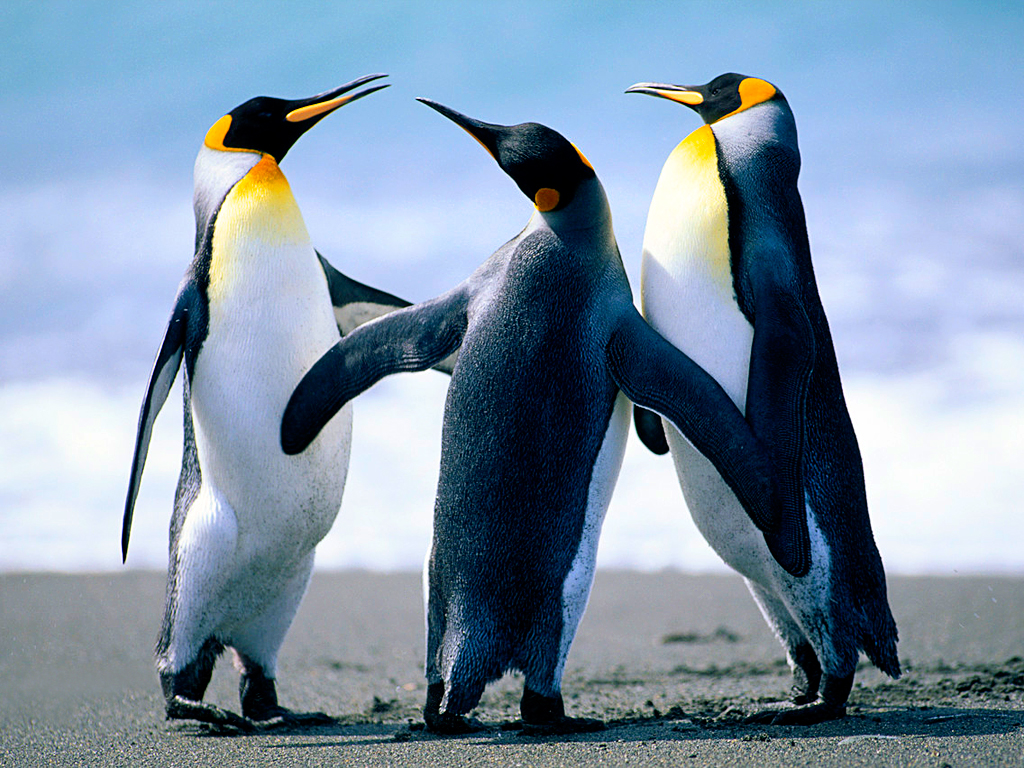
\includegraphics[scale=.50]{figures/Penguins.jpg}
\caption{TAMU figure}
\label{fig:tamu-fig6}
\end{figure}

\section{Appendix Section}


\pagebreak{}
\end{appendices}
\end{document} 
